\documentclass[sigconf,nonacm]{acmart}
\usepackage{kk-acm}

\settopmatter{printfolios=true}

\begin{document}

\title{Kinetic-KAN: Solver-Aware Neural Dynamics}
\subtitle{Project Final Report \textperiodcentered{} Group A\_08, Section A}

\author{Nawriz Ahmed Turjo}
\affiliation{%
  \department{Student ID 2105032}
  \institution{Bangladesh University of Engineering and Technology}
  \city{Dhaka}
  \country{Bangladesh}}

\author{Abhishek Roy}
\affiliation{%
  \department{Student ID 2105033}
  \institution{Bangladesh University of Engineering and Technology}
  \city{Dhaka}
  \country{Bangladesh}}

\author{Monjur Hossain Khan (Shovon)}
\affiliation{%
  \department{Student ID 2105043}
  \institution{Bangladesh University of Engineering and Technology}
  \city{Dhaka}
  \country{Bangladesh}}

\author{Shams Hossain Simanto}
\affiliation{%
  \department{Student ID 2105048}
  \institution{Bangladesh University of Engineering and Technology}
  \city{Dhaka}
  \country{Bangladesh}}

\author{Md.\ Abrar Jahin}
\affiliation{%
  \department{Student ID 2105055}
  \institution{Bangladesh University of Engineering and Technology}
  \city{Dhaka}
  \country{Bangladesh}}

\renewcommand{\shortauthors}{Group A\_08}

\begin{abstract}
Kolmogorov-Arnold Network ODEs (KAN-ODEs) replace the multilayer perceptron
inside a Neural ODE with a network whose every edge is a learnable univariate
function. We reproduce the Lotka-Volterra benchmark of the KAN-ODE base paper
in PyTorch, implementing six explicit Runge-Kutta integrators and seven basis
families from their defining formulas and verifying every integrator's order
to round-off. We then treat the paper's three fixed design choices
(integrator, basis and gradient method) as variables, extend the recipe to a
damped pendulum, an SIR epidemic model and a non-mechanistic outbreak curve, and run
follow-on studies on adjoint sensitivity, gradient dynamics, a learnable
basis blend, solver stiffness and sparse symbolic regression. Above order
two, the solver does not change accuracy: Midpoint matches Tsit5 within
$0.3\%$ at $29\%$ of the cost. Networks learn the field their solver needs
(the Euler-trained model matches the inverse modified equation), and every
trained model, KAN or MLP, is an attracting limit cycle rather than the true
neutral centre. At $10^4$ epochs KAN-ODE extrapolates $5.4\times$ better
than a parameter-matched MLP, but at $5\times10^4$ epochs the MLP is
$6.8\times$ better. B-spline and RBF bases are tied, while global polynomials
extrapolate $4$--$5\times$ worse. SIR's training failure traces to a
$19\times$ unit-scale mismatch at initialization; time rescaling, a
conservation projection and a vanishing-field gate move extrapolation $R^2$
from $-20.97$ to $+0.998$. All results are single-seed.

\smallskip\noindent\textbf{Code:} \url{https://github.com/NawrizTurjo/kinetic-kan}
\end{abstract}

\keywords{Kolmogorov-Arnold networks, neural ordinary differential equations,
Runge-Kutta methods, basis functions, numerical stability, extrapolation}

\maketitle

\section{Introduction and Base Paper Review}
\label{sec:introduction}
A Neural ODE \cite{chen2018neuralode} learns an unknown dynamical system
$\dot{\mathbf{u}}(t) = \mathbf{F}(\mathbf{u}(t))$ by fitting a vector field
$\mathbf{f}_\theta(\mathbf{u}(t))$ and integrating it numerically. The usual
choice for $\mathbf{f}_\theta$ is a multilayer perceptron (MLP), with fixed
activations on the nodes and all learnable structure in the linear weights,
$\mathbf{y} = \sigma(\mathbf{W}\mathbf{x}+\mathbf{b})$. A Kolmogorov-Arnold
Network (KAN) \cite{liu2024kan} flips this around: every \emph{edge} carries
its own learnable univariate function $\phi(x)$, and each node just sums its
incoming edges, $y_j = \sum_i \phi_{i,j}(x_i)$. The idea comes from the
Kolmogorov-Arnold representation theorem, which says that any continuous
multivariate function on a bounded domain can be written as a finite
composition of continuous univariate functions and addition,
\begin{equation}
f(\mathbf{x}) = \sum_{q=1}^{2n+1}\Phi_q\!\left(\sum_{p=1}^{n}\phi_{q,p}(x_p)\right),
\label{eq:kolmogorov-arnold}
\end{equation}
so no nonlinearity has to be fixed in advance; the network learns the shape
of each univariate function. In practice each edge function is a fixed
smooth residual plus a learnable expansion in a chosen basis. In the form we
implement,
\begin{equation}
\phi(x) = w_b\, b(x) + \sum_{i=1}^{G} c_i\, B_i\big(\mathrm{norm}(x)\big),
\label{eq:kan-edge}
\end{equation}
with $b(x)=\mathrm{silu}(x) = x/(1+e^{-x})$ and $\mathrm{norm}(x)=\tanh x$.
Here $B_1,\dots,B_G$ are $G$ basis functions attached to a uniform grid of
knots $z_g\in[-1,1]$ with spacing $h=2/(G-1)$, the $c_i$ are trainable
coefficients, and $w_b$ weights the residual. (The original \texttt{pykan}
form carries $G+k$ spline functions and a separate scale $w_s$ on the
expansion; with one coefficient per basis function that scale is redundant,
so we drop it.) The choice of $B_i$ is a design decision rather than a
mathematical necessity. A Gaussian radial basis function (RBF) grid,
$B_i(u)=\exp(-(u-z_i)^2/2h^2)$, gives each edge smooth support that decays
quickly but never reaches zero. A degree-$k$ B-spline built by the
Cox-de Boor recursion instead gives each edge compact local support, exactly
zero outside its own knot span.

\subsection{The base paper: KAN-ODEs}
\label{sec:base-paper}

Koenig et al.\ \cite{Koenig_2024} put this construction inside a Neural
ODE's vector field, $\dot{\mathbf{u}}=\mathbf{f}_\theta(\mathbf{u})$ with
every edge of $\mathbf{f}_\theta$ built from Equation~\ref{eq:kan-edge}, and
obtain the trajectory by numerically integrating that field forward in time.
On the Lotka-Volterra predator-prey system they report two central claims:
a KAN-ODE with 240 parameters extrapolates the system's oscillation
accurately from a short training window, and it reaches a target training
loss in roughly $10^4$ epochs where a parameter-matched (252-parameter)
MLP-based Neural ODE needs $10^5$, a tenfold training-speed advantage. The
paper also applies KAN-ODEs to other systems, including inferring hidden
physics; we focus on its Lotka-Volterra benchmark.

To get these results the paper commits to three design decisions, which we
treat as free variables:
\begin{enumerate}
\item the \textbf{integrator}: an adaptive fifth-order Runge-Kutta method,
  Tsit5 \cite{tsitouras2011tsit5};
\item the \textbf{basis}: Gaussian RBF;
\item the \textbf{differentiation method} used to get gradients through the
  integrator: continuous adjoint sensitivity, chosen for its constant memory
  cost in trajectory length.
\end{enumerate}
The basis choice is not something we invented to vary. The original KAN
paper \cite{liu2024kan} used cubic B-splines by default, and the base paper
switched to Gaussian RBF for the ODE setting because its derivative never
vanishes, which matters once the edge function sits inside a differentiated
integrator rather than a static regression. We restore B-spline and add five
further bases, so the trade-off behind that switch is measured rather than
assumed.

\subsection{Why training needs to be studied, not just the final error}

Besides Lotka-Volterra, we use two textbook systems, the SIR epidemic model
and a damped pendulum, chosen because their governing equations are simple
and well understood. Any training failure can then be blamed on the
architecture or the optimization rather than on ambiguous target dynamics.
The integrator's interaction with training is not predictable from classical
numerical analysis alone, because the integrator sits inside a
backpropagation graph rather than a standalone forward solve: a solver that
is perfectly stable in the classical sense can still train badly, train to a
wrong answer, or fail to generalize. Section~\ref{sec:numerics} makes this
concrete. A network trained through Forward Euler learns the \emph{inverse
modified equation} of backward error analysis rather than the physical
field, and every trained model, KAN or MLP, replaces Lotka-Volterra's family
of neutral orbits with a single attracting limit cycle. Diagnosing behaviour
like this means treating training itself as an object of study.

\subsection{Summary of our work}
\label{sec:work-summary}

Table~\ref{tab:work-summary} lists every study we ran, why we ran it, what we
found, and where it is reported. In short, our objectives were to:
(i)~reproduce the base paper's Lotka-Volterra benchmark with every
integrator and basis implemented and verified from its defining
formula\footnote{Code, trained checkpoints and the analysis pipeline are
available at \url{https://github.com/NawrizTurjo/kinetic-kan}.};
(ii)~vary each of the paper's three fixed design choices and measure what
it actually costs or buys; (iii)~check whether the recipe transfers to other
dynamical systems, and fix it where it does not; and (iv)~test whether our
conclusions survive a five times larger training budget.

\begin{table*}[t]
\centering
\footnotesize
\renewcommand{\arraystretch}{1.18}
\caption{Summary of the studies in this report.}
\label{tab:work-summary}
\begin{tabularx}{\textwidth}{|C{0.35cm}|L{2.6cm}|L{4.5cm}|Y|C{0.6cm}|}
\hline
\hdrrow \thh{\#} & \thh{Study} & \thh{Why we ran it} & \thh{What we observed} & \thh{Sec.}\\
\hline
1 & Baseline reproduction: KAN-ODE vs.\ MLP-ODE & Test the base paper's two headline claims (accuracy and training speed) at matched parameter count. & KAN-ODE extrapolates $5.4\times$ better at $10^4$ epochs, a gap explained by a $48\times$ smaller period error. The MLP trains $4.1\times$ \emph{faster}. The paper's literal tanh MLP trains only under the paper's own learning rate and initialization. & \ref{sec:kan-vs-mlp}\\
\hline
2 & Integrator ablation & The paper fixes Tsit5; does solver order matter for training? & All six solvers pass their order conditions to round-off. Above order two, accuracy is flat: Midpoint matches Tsit5 within $0.3\%$ at $29\%$ of the cost. The Euler model learns the inverse modified equation, and no model transfers across solver families. & \ref{sec:solver-results}\\
\hline
3 & Basis-function ablation & The paper switched from B-spline to RBF; is that justified? & B-spline and RBF are tied, with RBF $3.9\times$ cheaper. Global polynomials extrapolate $4$--$5\times$ worse. Locality, not conditioning, separates the bases. & \ref{sec:basis-results}\\
\hline
4 & Step-size and noise sensitivity & How sensitive is the fit to sampling density and observation noise? & Step size acts as a data-density choice (non-monotone). Extrapolation MSE scales as $12.9\,\sigma^{2.02}$ with noise. & \ref{sec:dt-noise}\\
\hline
5 & What the trained fields learned & Does low trajectory error mean the right vector field? & No. Every model is an attracting limit cycle around a spurious unstable equilibrium, accurate only in a thin tube around the training orbit. & \ref{sec:numerics}\\
\hline
6 & Cross-domain failures and fixes & Does the Lotka-Volterra recipe transfer to the pendulum and SIR? & A longer training window fixes the pendulum. SIR's $19\times$ scale mismatch at initialization is fixed by time rescaling and a conservation projection; adding a vanishing-field gate gives $R^2$: $-20.97\to+0.998$. The KAN advantage widens to $40.6\times$ at twice the horizon. & \ref{sec:crossdomain}\\
\hline
7 & Adjoint vs.\ direct autograd & The paper uses the adjoint for its memory saving; does that matter at our scale? & The adjoint uses less memory at every length tested but is $1.9$--$2.1\times$ slower, so we use direct autograd. & \ref{sec:track-a}\\
\hline
8 & Gradient-norm dynamics & Is Euler's convergence floor caused by noisier gradients? & No ($\rho=-0.088$, $p=0.87$); gradient spike bursts are shared across all solvers. & \ref{sec:track-b}\\
\hline
9 & Learnable hybrid basis & Can the network learn its own B-spline/RBF blend? & The gate works as designed but never beats the better pure basis, and it overfits on the pendulum past 3000 epochs. & \ref{sec:track-c}\\
\hline
10 & Stiffness--solver map & Do explicit solvers fail as the pendulum's damping grows? & Zero divergences, as linear stability predicts. The failures trace to the random seed and a spurious learned equilibrium. & \ref{sec:track-d}\\
\hline
11 & Sparse regression and epidemic transfer & How does KAN-ODE compare with SINDy under noise, and do the SIR fixes transfer to a non-mechanistic outbreak curve? & KAN-ODE is more accurate at every noise level, but degrades $1540\times$ against SINDy's $9\times$. Pruning finds no sparse structure. Two of three SIR fixes transfer. & \ref{sec:track-e}\\
\hline
12 & Epoch-budget validation & Do the $10^4$-epoch conclusions survive five times the budget? & Solver and basis rankings hold. KAN vs.\ MLP \emph{reverses}: the MLP is $6.8\times$ better at $5\times10^4$ epochs. & \ref{sec:phase4}\\
\hline
13 & Comparison with the base paper & Audit our recipe against the paper field by field. & Architecture and basis match. The KAN's training speed is reproduced within $1.4\times$. The tenfold speed advantage depends on the MLP baseline's optimizer settings. & \ref{sec:audit}\\
\hline
\end{tabularx}
\end{table*}

The rest of the paper follows the course's required structure.
Section~\ref{sec:method} gives the numerical methods: the KAN-ODE model, the
integrators, the basis families, the two gradient methods, the hybrid basis
and sparse regression. Section~\ref{sec:impl} describes the datasets,
training recipe, evaluation protocol and compute budget.
Section~\ref{sec:results} reports each study in the order of
Table~\ref{tab:work-summary}, compares our findings with the base paper, and
discusses the patterns that recur across studies.
Section~\ref{sec:conclusion} concludes with limitations and future work.


\section{Methodology}
\label{sec:method}
\subsection{The KAN-ODE model}
\label{sec:architecture}

Every KAN-ODE we train has the same architecture: a two-layer network with
widths $[2,10,2]$, each edge carrying the expansion of
Equation~\ref{eq:kan-edge} over a grid of $G=5$ basis functions. It is
wrapped inside an explicit Runge-Kutta integrator that advances the state
and hands the resulting trajectory to the loss.
Figure~\ref{fig:kan-ode-architecture} shows the full training loop and marks
the three components we vary.

\begin{figure*}[t]
\centering
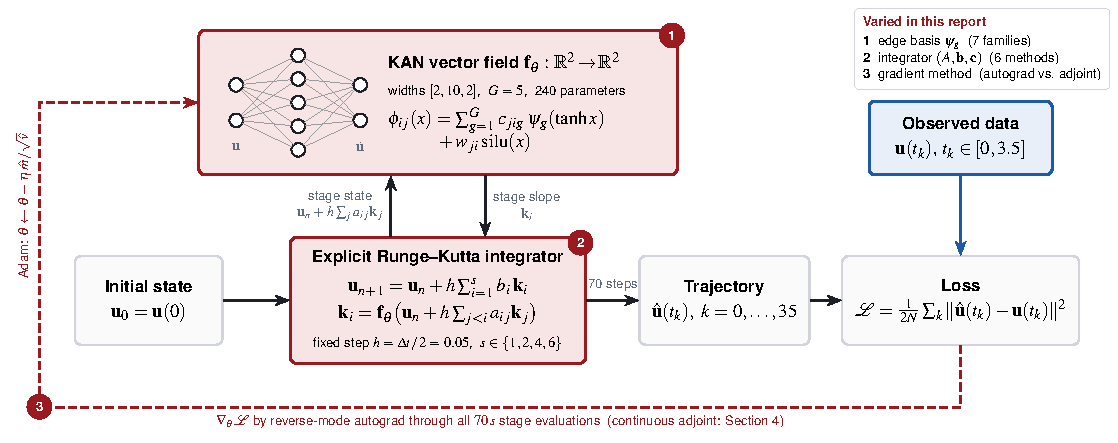
\includegraphics[width=\textwidth]{figures/tikz/kan_ode_system.pdf}
\caption{The KAN-ODE training loop as implemented. The integrator calls the
network once per Runge-Kutta stage, so one training epoch on $[0,3.5]$
evaluates $\mathbf{f}_\theta$ $70s$ times ($35$ sampling intervals, two
sub-steps each, $s$ stages per step). The loss gradient comes from
differentiating through every one of those evaluations. Numbered badges mark
the three components we vary: the edge basis
(Sections~\ref{sec:basis-results} and~\ref{sec:track-c}), the integrator
(Sections~\ref{sec:solver-results}, \ref{sec:track-b} and~\ref{sec:track-d})
and the gradient method (Section~\ref{sec:track-a}).}
\label{fig:kan-ode-architecture}
\end{figure*}

\subsubsection{One KAN layer as two matrix products}

The network is two KDense layers. For a batch
$\mathbf{X}\in\mathbb{R}^{B\times d_{\text{in}}}$, a layer evaluates every
edge function of Equation~\ref{eq:kan-edge} at once:
\begin{equation}
\Psi_{b,i,g} = B_g\big(\tanh X_{b,i}\big), \qquad
\mathbf{Y} = \underbrace{\Psi_{\text{flat}}\,\mathbf{C}^{\top}}_{\text{spline branch}}
           + \underbrace{\mathrm{silu}(\mathbf{X})\,\mathbf{W}^{\top}}_{\text{base branch}},
\label{eq:kdense}
\end{equation}
with $\mathbf{C}\in\mathbb{R}^{d_{\text{out}}\times d_{\text{in}}G}$ and
$\mathbf{W}\in\mathbb{R}^{d_{\text{out}}\times d_{\text{in}}}$. Here
$\Psi_{\text{flat}}\in\mathbb{R}^{B\times d_{\text{in}}G}$ is $\Psi$ with
its last two axes merged. Entry $C_{j,(i,g)}$ is the coefficient $c_g$ of
edge $i\to j$ and $W_{j,i}$ is that edge's residual weight $w_b$, so
$Y_{b,j}=\sum_i\phi_{i,j}(X_{b,i})$ exactly. Figure~\ref{fig:kdense} traces
the tensor shapes. The forward pass is short enough to show in full:

\begin{pycode}[Forward pass of one KDense layer]
x_flat = x.view(-1, self.in_features)          # [B, d_in]
x_norm = self.normalizer(x_flat)               # tanh -> [-1, 1]
basis_vals = self.basis_func(x_norm, self.grid, self.denominator)
basis_flat = basis_vals.reshape(basis_vals.size(0),
                                self.in_features * self.grid_len)
spline_out = F.linear(basis_flat, self.C)      # Psi_flat @ C^T
if self.use_base_act and self.W is not None:
    base_val = self.base_act(x_flat)           # silu(x)
    base_out = F.linear(base_val, self.W)      # silu(x) @ W^T
    out = spline_out + base_out
else:
    out = spline_out
return out.view(*orig_shape[:-1], self.out_features)
\end{pycode}

\begin{figure*}[t]
\centering
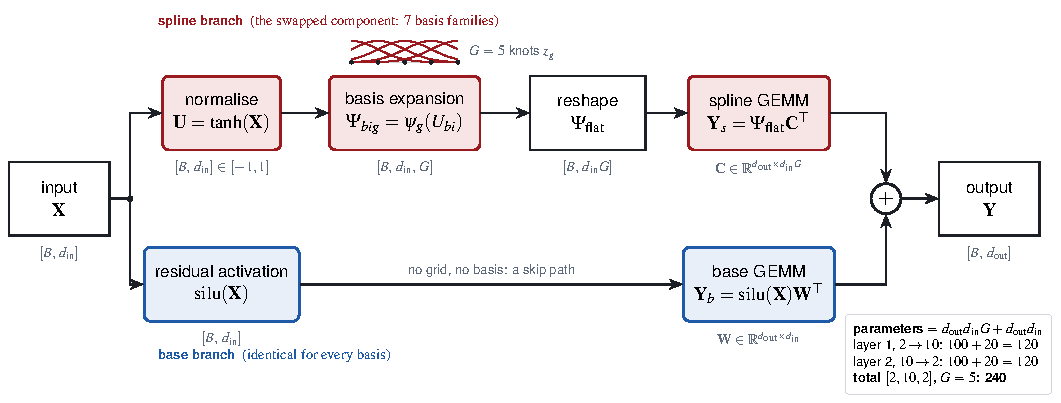
\includegraphics[width=0.9\textwidth]{figures/tikz/kdense_layer.pdf}
\caption{Tensor flow through one KDense layer
(Equation~\ref{eq:kdense}). Only the basis-expansion step differs between
the seven basis families of Section~\ref{sec:bases}; every basis function
has the same signature,
$(\mathbf{U},\mathbf{z},h)\mapsto\Psi\in\mathbb{R}^{B\times d_{\text{in}}\times G}$,
so swapping the basis changes one tensor and nothing else.}
\label{fig:kdense}
\end{figure*}

\paragraph{Parameter count.} Each layer holds
$d_{\text{out}}d_{\text{in}}G$ spline coefficients,
$d_{\text{out}}d_{\text{in}}$ residual weights and no bias. For $[2,10,2]$
with $G=5$, layer one ($2\to10$) has $10\cdot2\cdot5+10\cdot2=120$
parameters and layer two ($10\to2$) has $2\cdot10\cdot5+2\cdot10=120$, for
the $240$ total the base paper reports. The comparison MLPs of
Section~\ref{sec:kan-vs-mlp} are sized to match: the paper's $[2,50,2]$
network has $2\cdot50+50+50\cdot2+2=252$ parameters, and the deeper
$[2,14,8,8,2]$ network we use as the working baseline also has
$(28+14)+(112+8)+(64+8)+(16+2)=252$.

\paragraph{Why the \texttt{efficient-kan} formulation.} The reference
implementation, \texttt{pykan} \cite{liu2024kan}, represents every edge with
its own spline object and recomputes the grid during training. Inside a
Neural ODE that cost is multiplied by the integrator: one epoch of Tsit5 on
the training window calls $\mathbf{f}_\theta$ $420$ times, and reverse-mode
differentiation keeps every one of those calls in the autograd graph. Our
layer follows the \texttt{efficient-kan} reformulation
\cite{blealtan2024efficientkan} instead: the knots are a fixed buffer, the
basis is evaluated for all edges with one broadcast, and the contraction is
one dense matrix product per branch (Equation~\ref{eq:kdense}). Each stage
therefore adds two matrix multiplications and a handful of elementwise
operations to the graph, however many edges there are. The same structure
makes every basis we substitute into Equation~\ref{eq:kan-edge} (RBF,
B-spline, Chebyshev, Lagrange, Newton, IQF, RSWAF) a swappable tensor rather
than a different object type.

\paragraph{What we implemented ourselves.} We wrote the KAN layer, the seven
basis functions, the six fixed-step Runge-Kutta integrators, the
invariant-enforcing field wrappers used for SIR and the training loop
directly in PyTorch \cite{paszke2019pytorch}, rather than importing them, so
that every basis and solver could be instrumented in the same way. The
integrators apply the tableaux of Section~\ref{sec:integrators} verbatim.
Tsit5 and DOPRI5 run at a fixed step with their fifth-order weights only,
whereas the base paper uses Tsit5's embedded error estimate for adaptive
step control. The base paper compiles its integration loop in Julia's SciML
ecosystem; we run the same loop uncompiled in PyTorch because it was simpler
for us to work with. Our wall-clock figures are therefore comparable across
our own runs but not against the paper's reported times
(Section~\ref{sec:budget} quantifies what this costs).

\subsection{Runge-Kutta integrators}
\label{sec:integrators}

Every integrator we use is an explicit Runge-Kutta method: one step of size
$h$ evaluates $s$ stage slopes and combines them,
\begin{equation}
\mathbf{k}_i=\mathbf{f}_\theta\Big(\mathbf{u}_n+h\sum_{j=1}^{i-1}a_{ij}\mathbf{k}_j\Big),
\qquad
\mathbf{u}_{n+1}=\mathbf{u}_n+h\sum_{i=1}^{s}b_i\mathbf{k}_i,
\label{eq:rk-general}
\end{equation}
for $i=1,\dots,s$, so a method is fully specified by its Butcher tableau
$(A,\mathbf{b},\mathbf{c})$ with $c_i=\sum_j a_{ij}$. Writing
$\mathbf{u}_n$ for the state at step $n$, the four low-order methods are
\begin{align}
\text{Euler ($p=1$):}\ & \mathbf{u}_{n+1} = \mathbf{u}_n + h\, \mathbf{f}_\theta(\mathbf{u}_n) \label{eq:euler}\\
\text{Midpoint ($p=2$):}\ & \mathbf{u}_{n+1} = \mathbf{u}_n + h\,\mathbf{f}_\theta\!\left(\mathbf{u}_n + \tfrac{h}{2}\mathbf{k}_1\right) \label{eq:midpoint}\\
\text{Heun ($p=2$):}\ & \mathbf{u}_{n+1} = \mathbf{u}_n + \tfrac{h}{2}(\mathbf{k}_1+\mathbf{k}_2),\ \ \mathbf{k}_2 = \mathbf{f}_\theta(\mathbf{u}_n+h\,\mathbf{k}_1) \label{eq:heun}\\
\text{RK4 ($p=4$):}\ & \mathbf{u}_{n+1} = \mathbf{u}_n + \tfrac{h}{6}\left(\mathbf{k}_1+2\mathbf{k}_2+2\mathbf{k}_3+\mathbf{k}_4\right) \label{eq:rk4}
\end{align}
with $\mathbf{k}_1=\mathbf{f}_\theta(\mathbf{u}_n)$ throughout and the
classical RK4 stages
$\mathbf{k}_2=\mathbf{f}_\theta(\mathbf{u}_n+\tfrac{h}{2}\mathbf{k}_1)$,
$\mathbf{k}_3=\mathbf{f}_\theta(\mathbf{u}_n+\tfrac{h}{2}\mathbf{k}_2)$,
$\mathbf{k}_4=\mathbf{f}_\theta(\mathbf{u}_n+h\,\mathbf{k}_3)$. DOPRI5 and
Tsit5 are both seven-stage 5(4) embedded pairs whose seventh stage exists
only to supply the fourth-order error estimate (the ``first same as last''
stage); its fifth-order weight is $b_7=0$. At a fixed step, as here, the
seventh evaluation contributes nothing to the update, so our implementation
skips it and both methods cost \emph{six} evaluations per step. Their
coefficients satisfy all $17$ order conditions up to order five, and
Tsitouras \cite{tsitouras2011tsit5} additionally minimised the size of the
sixth-order error terms. Table~\ref{tab:tsit5} lists the Tsit5 coefficients
exactly as implemented, and Figure~\ref{fig:rk-stages} shows where each
method samples the field within one step. Every extra stage costs one more
evaluation of $\mathbf{f}_\theta$, which is why we measure cost in function
evaluations per epoch rather than by solver order alone.

\begin{table}[t]
\centering
\scriptsize
\setlength{\tabcolsep}{2.6pt}
\renewcommand{\arraystretch}{1.15}
\caption{Fixed-step Tsit5 tableau as implemented (first six stages, rounded
to six significant figures; the code carries 16). Row $i$ lists $c_i$ and
$a_{i1},\dots,a_{i,i-1}$; the last two rows list the solution weights $b_i$.}
\label{tab:tsit5}
\begin{tabular}{@{}r|rrrrr@{}}
$0$ & & & & & \\
$0.161$ & $0.161$ & & & & \\
$0.327$ & $-0.00848066$ & $0.335481$ & & & \\
$0.9$ & $2.89715$ & $-6.35945$ & $4.36230$ & & \\
$0.980026$ & $5.32586$ & $-11.7489$ & $7.49554$ & $-0.0924951$ & \\
$1$ & $5.86146$ & $-12.9210$ & $8.15937$ & $-0.0715850$ & $-0.0282691$\\
\hline
$\mathbf{b}^\top$ & $0.0964608$ & $0.01$ & $0.479890$ & $1.37901$ & $-3.29007$\\
 & $2.32471$ & & & & \\
\end{tabular}
\end{table}

\begin{figure}[t]
\centering
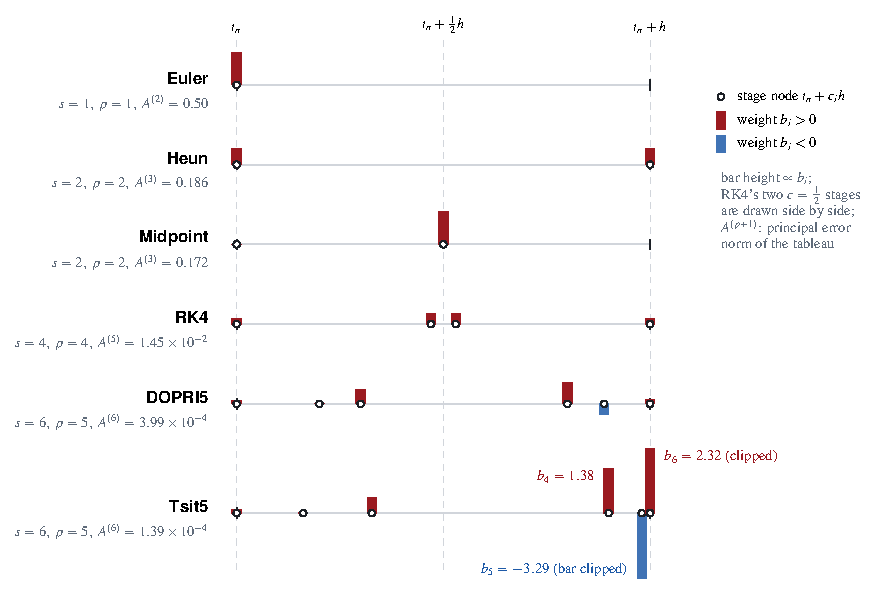
\includegraphics[width=\columnwidth]{figures/tikz/rk_stages.pdf}
\caption{Stage nodes $t_n+c_ih$ and solution weights $b_i$ of the six
implemented methods, drawn from the coefficients in the code. Heun and
Midpoint use the same number of evaluations but sample at opposite places:
Heun averages the two ends of the step, Midpoint uses only a slope at its
centre. Tsit5 reaches order five with large weights of both signs
($b_5=-3.29$), a cancellation that is harmless in exact arithmetic and buys
its small error constant.}
\label{fig:rk-stages}
\end{figure}

\subsection{Basis functions}
\label{sec:bases}

Writing $z_g$ for the $g$-th of $G$ evenly spaced grid centres with spacing
$h=2/(G-1)$, and $u=\tanh(x)\in[-1,1]$ for the normalized edge input, the
seven bases we compare are, exactly as implemented,
\begin{gather}
B_g^{\text{RBF}}(u)=\exp\!\left(-\tfrac12\left(\tfrac{u-z_g}{h}\right)^2\right),\quad
B_g^{\text{IQF}}(u)=\frac{1}{1+\left(\frac{u-z_g}{h}\right)^2}, \nonumber\\
B_g^{\text{RSWAF}}(u)=1-\tanh^2\!\left(\tfrac{u-z_g}{h}\right),
\label{eq:basis-rbf-spline}
\end{gather}
\begin{gather}
B_g^{\text{Cheb}}(u)=T_{g-1}(u)=\cos\big((g-1)\arccos u\big), \nonumber\\
B_g^{\text{Lag}}(u)=\prod_{j\neq g}\frac{u-z_j}{z_g-z_j}, \qquad
B_g^{\text{Newt}}(u)=\prod_{j<g}(u-z_j),
\label{eq:basis-poly}
\end{gather}
plus the cubic B-spline $B_g^{\text{spline}}$, built by the Cox--de Boor
recursion from degree-0 indicator functions by repeated linear blending,
\begin{gather}
B_{g,0}(u)=\mathbf{1}[t_g\le u<t_{g+1}], \nonumber\\
B_{g,p}(u)=\frac{u-t_g}{t_{g+p}-t_g}B_{g,p-1}(u)+\frac{t_{g+p+1}-u}{t_{g+p+1}-t_{g+1}}B_{g+1,p-1}(u),
\label{eq:cox-de-boor}
\end{gather}
on the clamped knot vector $\mathbf{t}=(-1,-1,-1,-1,0,1,1,1,1)$ for $G=5$,
$k=3$. The clamping makes the five splines a partition of unity with
$B_1(-1)=B_5(1)=1$, and it is what gives the spline compact support:
$B_{g,k}(u)=0$ outside the $k+2$ knots the recursion references. Gaussian
RBF, IQF and RSWAF are local but never exactly zero. Chebyshev, Lagrange and
Newton have no locality at all: every coefficient $c_g$ influences $\phi(x)$
at every $x$. The residual term $w_b\,\mathrm{silu}(x)$ in
Equation~\ref{eq:kan-edge} is the same for every basis, since it is a fixed
part of the edge parameterization rather than one of the substituted terms.

\subsection{Computing gradients: direct autograd and the adjoint method}
\label{sec:gradients}

There are two ways to compute gradients through a Neural ODE. \textbf{Direct
autograd} treats the numerical integrator as an ordinary computational
graph: each of the solver's $N_t$ forward steps is recorded, and the reverse
pass walks back through every recorded step, so peak memory grows linearly
with the number of steps. \textbf{Adjoint sensitivity}
\cite{chen2018neuralode} instead treats the forward solve as a black box and
derives a second, augmented ODE that produces the same gradient without
storing the intermediate states. Writing $\mathbf{a}(t) = \partial
L/\partial\mathbf{u}(t)$ for the adjoint state, it satisfies its own
backward-time differential equation,
\begin{equation}
\frac{d\mathbf{a}}{dt} = -\mathbf{a}^\top\frac{\partial \mathbf{f}_\theta}{\partial\mathbf{u}},
\qquad
\frac{dL}{d\theta} = \int_{t_1}^{t_0}\mathbf{a}^\top\frac{\partial\mathbf{f}_\theta}{\partial\theta}\,dt,
\label{eq:adjoint}
\end{equation}
solved backward from $t_1$ to $t_0$ alongside the original state
$\mathbf{u}(t)$, which is recomputed rather than stored. Memory then depends
only on the size of the state and parameter vectors, not on how many steps
the forward solve took: $O(1)$ in trajectory length, against direct
autograd's $O(N_t)$ (Figure~\ref{fig:adjoint-schematic}). All our training
runs use direct autograd; Section~\ref{sec:track-a} measures whether that
choice is justified.

\begin{figure}[t]
\centering
\resizebox{\columnwidth}{!}{%
\begin{tikzpicture}[
  font=\small,
  statend/.style={draw=ink, fill=accentsoft, minimum width=9mm, minimum height=7mm, rounded corners=2pt},
  adjnd/.style={draw=ink!60, fill=codebg, minimum width=11mm, minimum height=7mm, rounded corners=2pt},
  arr/.style={-{Stealth[length=2.2mm]}, draw=ink!70, thick},
  panellbl/.style={font=\small\sffamily\bfseries\color{ink}}
]
  \node[statend] (u0) at (0,0) {$u_0$};
  \foreach \i/\x in {1/1.5,2/3.0,3/4.5,4/6.0} {
    \node[statend] (u\i) at (\x,0) {$u_\i$};
  }
  \draw[arr] (u0) -- (u1); \draw[arr] (u1) -- (u2);
  \draw[arr] (u2) -- (u3); \draw[arr] (u3) -- (u4);
  \draw[{Stealth[length=2.2mm]}-, dashed, accent, thick]
    (u0.south) .. controls +(0,-0.9) and +(0,-0.9) .. (u4.south)
    node[midway, below, font=\scriptsize\sffamily\color{accent}] {backward pass walks every stored $u_i$};
  \node[panellbl] at (3.0,0.75) {Direct autograd: every $u_i$ stored, $O(N_t)$ memory};
  \begin{scope}[yshift=-2.6cm]
    \node[adjnd] (a0) at (0,0) {$\mathbf{a}(t_0)$};
    \node[adjnd] (a1) at (6.0,0) {$\mathbf{a}(t_1)$};
    \draw[arr, ink!65] (a1) -- (a0);
    \node[font=\scriptsize\sffamily\color{ink!70}] at (3.0,0.3) {adjoint ODE (Eq.~\ref{eq:adjoint}) integrated backward};
    \node[font=\scriptsize\sffamily\color{ink!70}] at (3.0,-0.3) {$u(t)$ recomputed as needed, nothing stored};
    \node[panellbl] at (3.0,0.75) {Adjoint sensitivity: $O(1)$ memory, independent of $N_t$};
  \end{scope}
\end{tikzpicture}}
\caption{Direct autograd (top) keeps every intermediate state $u_i$ in memory
so the backward pass can reuse it, giving $O(N_t)$ memory. Adjoint
sensitivity (bottom) instead solves the backward-time equation of
Equation~\ref{eq:adjoint}, recomputing $u(t)$ as needed, giving $O(1)$
memory regardless of $N_t$.}
\label{fig:adjoint-schematic}
\end{figure}

\subsection{A learnable hybrid basis}
\label{sec:hybrid-method}

Rather than choosing one basis function $B_i(x)$ in
Equation~\ref{eq:kan-edge} in advance, we can make the choice itself a
trained quantity: a learnable convex blend of two candidate bases inside
every edge,
\begin{equation}
\phi(x) = \alpha\cdot\mathrm{Spline}(x) + \beta\cdot\mathrm{RBF}(x),
\qquad (\alpha,\beta) = \operatorname{softmax}(\text{logits}),
\label{eq:hybrid-basis}
\end{equation}
trained end-to-end from a neutral start ($\alpha=\beta=0.5$) with no
hand-set schedule (Figure~\ref{fig:hybrid-schematic}). We produce the blend
weights with a softmax over two learnable logits rather than, say, a single
sigmoid-gated weight, because a softmax guarantees $\alpha+\beta=1$ by
construction. The two bases then always form a genuine convex combination,
so the gate can only trade one basis off against the other instead of
scaling the whole edge output up or down as a side effect. One pair of
logits is shared across every edge, so the model learns a single global
blend. This keeps the number of new parameters at two; it is a
simplification, not a claim that per-edge blending would fail.

\begin{figure}[t]
\centering
\resizebox{\columnwidth}{!}{%
\begin{tikzpicture}[node distance=10mm, font=\small,
  boxnd/.style={draw=ink, fill=accentsoft, minimum size=7mm, rounded corners=2pt},
  fnbox/.style={draw=ink!60, fill=codebg, minimum width=20mm, minimum height=7mm, rounded corners=2pt},
  gatend/.style={draw=accent, fill=white, circle, minimum size=6mm, inner sep=0pt, font=\bfseries\small\color{accent}},
  sumnd/.style={draw=accent, fill=accentsoft, circle, minimum size=7mm, inner sep=0pt, font=\bfseries\color{accent}},
  arr/.style={-{Stealth[length=2mm]}, draw=ink!65, thick}
]
  \node[boxnd] (x) at (0,0) {$x$};
  \node[fnbox] (sp) at (2.6,1.1) {$\mathrm{Spline}(x)$};
  \node[fnbox] (rbf) at (2.6,-1.1) {$\mathrm{RBF}(x)$};
  \node[gatend] (gA) at (5.0,1.1) {$\times$};
  \node[gatend] (gB) at (5.0,-1.1) {$\times$};
  \node[sumnd] (sum) at (7.2,0) {$+$};
  \node[boxnd] (phi) at (9.2,0) {$\phi(x)$};
  \node[fnbox, minimum width=19mm, minimum height=6mm, font=\scriptsize] (softmax) at (2.6,0) {$\operatorname{softmax}(\text{logits})$};
  \draw[arr] (x) -- (sp);
  \draw[arr] (x) -- (rbf);
  \draw[arr] (sp) -- (gA);
  \draw[arr] (rbf) -- (gB);
  \draw[arr] (gA) -- (sum);
  \draw[arr] (gB) -- (sum);
  \draw[arr] (sum) -- (phi);
  \draw[arr, accent!85] (softmax.north) -- node[right, font=\scriptsize\sffamily\color{accent!85}, pos=0.7]{$\alpha$} (gA.south);
  \draw[arr, accent!85] (softmax.south) -- node[right, font=\scriptsize\sffamily\color{accent!85}, pos=0.7]{$\beta$} (gB.north);
\end{tikzpicture}}
\caption{The hybrid-basis edge of Equation~\ref{eq:hybrid-basis}: every edge
evaluates both bases in parallel, and a shared softmax gate produces the
scalar weights $\alpha,\beta$ that multiply each basis's output before they
are summed into $\phi(x)$.}
\label{fig:hybrid-schematic}
\end{figure}

\subsection{Sparse regression and edge pruning}
\label{sec:sparse-method}

As a baseline from a completely different modelling approach, we use Sparse
Identification of Nonlinear Dynamics (SINDy) \cite{brunton2016sindy},
through the PySINDy library \cite{kaptanoglu2022pysindy}. SINDy fits a
governing equation as a sparse linear combination of candidate terms from a
fixed library; ours is every polynomial in $x$ and $y$ up to degree two,
$\{1,x,y,x^2,xy,y^2\}$. The coefficients are estimated by sequentially
thresholded least squares: fit by ordinary least squares against
numerically estimated derivatives, zero out every coefficient below a fixed
threshold, and refit on the surviving terms until the active set stops
changing. This is what makes the recovered model sparse and, in principle,
readable: unlike the KAN's 240 free parameters, SINDy returns a short list
of surviving terms with numeric coefficients that can be compared directly
with the true equation's. We hold the threshold fixed across the whole noise
sweep so that the comparison measures noise sensitivity rather than
per-level tuning.

The closest KAN-ODE analogue is to encourage sparsity during training and
prune weak edges afterwards. The base paper does this by adding an $L_1$
penalty on the spline coefficients to the loss,
\begin{equation}
\mathcal{L} = \mathrm{MSE}(\mathbf{u}_{\text{true}}, \mathbf{u}_{\text{pred}}) + \lambda\sum_{i} |c_i|,
\label{eq:l1-sparsity}
\end{equation}
where $c_i$ ranges over every spline coefficient in
Equation~\ref{eq:kan-edge} and $\lambda$ trades trajectory accuracy against
how many edges the penalty drives toward zero. Every checkpoint we trained
used $\lambda=0$, the plain mean-squared-error term alone. To prune, we rank
each edge by its mean spline-coefficient magnitude and mask the weakest
(Section~\ref{sec:track-e}).


\section{Implementation and Experiments}
\label{sec:impl}
\subsection{Datasets}
\label{sec:datasets}

All training data except the epidemic curve are simulated from known
equations, with ground truth generated by SciPy's \cite{virtanen2020scipy}
DOP853 integrator at relative and absolute tolerance $10^{-12}$, far below
any error we report. Table~\ref{tab:datasets} summarises the four systems
and their train/test splits. Every accuracy number is computed only on the
test window, which the training loss never sees.

\paragraph{Lotka-Volterra (main benchmark).} The base paper's predator-prey
system \cite{Koenig_2024},
\begin{gather}
\dot u_1 = \alpha u_1 - \beta u_1 u_2, \qquad \dot u_2 = \delta u_1 u_2 - \gamma u_2,
\nonumber\\
(\alpha,\beta,\gamma,\delta) = (1.5,\,1.0,\,3.0,\,1.0),
\label{eq:lv}
\end{gather}
from $\mathbf{u}(0)=(1,1)$, sampled every $\Delta t=0.1$. We train on
$t\in[0,3.5]$ (36 points) and score strictly on $t\in(3.5,14.0]$ (105
unseen points). Extrapolation is scored this way because it is the only
meaningful test of whether the network learned the dynamics rather than
memorising the training window; a model that reproduces the 36 training
points can still be badly wrong about the system. Two properties of
Equation~\ref{eq:lv} serve as exact, model-independent checks later on. It
has a single interior equilibrium
$\mathbf{u}^\ast=(\gamma/\delta,\ \alpha/\beta)=(3,\,1.5)$, where the
Jacobian has purely imaginary eigenvalues $\pm i\sqrt{\alpha\gamma}=\pm2.121i$.
And it conserves the first integral
\begin{equation}
H(u_1,u_2)=\delta u_1-\gamma\ln u_1+\beta u_2-\alpha\ln u_2,
\qquad \frac{\dd H}{\dd t}=0,
\label{eq:lv-invariant}
\end{equation}
so every orbit is a closed level curve of $H$ and the phase plane is filled
with a continuous family of neutral cycles. The orbit through $(1,1)$ has
$H_0=2$ and period $T=3.3175$, so the training window covers $1.06$
periods, the test window $3.2$ further periods, and $[0,14]$ about $4.2$.

\paragraph{SIR epidemic model.} The compartmental model splits a fixed
population into susceptible ($S$), infected ($I$) and recovered ($R$)
fractions,
\begin{equation}
\dot S = -\beta S I, \quad \dot I = \beta S I - \gamma I, \quad \dot R = \gamma I,
\label{eq:sir}
\end{equation}
with $(\beta,\gamma)=(0.35,\,0.1)$ and $(S,I,R)(0)=(0.99,0.01,0)$. It has
a built-in algebraic invariant, $S+I+R=1$, because the three terms of the
field cancel when summed. The invariant holds for any parameter values, so a
model that violates it has learned a field with the wrong structure, not
merely an inaccurate one. We simulate $t\in[0,80]$ days at
$\Delta t=0.5$, train on $[0,50]$ (101 points) and test on $(50,80]$.

\paragraph{Damped pendulum.} The angle $\theta$ and angular velocity
$\omega$ evolve under gravity and viscous friction,
\begin{equation}
\dot\theta = \omega, \qquad \dot\omega = -\frac{g}{L}\sin\theta - \mu\,\omega,
\qquad (g/L,\,\mu) = (9.81,\,0.5),
\label{eq:pendulum}
\end{equation}
from $(\theta,\omega)(0)=(2,0)$. Since $\mu>0$, the mechanical energy
$E=\tfrac{1}{2}mL^2\omega^2 + mgL(1-\cos\theta)$ strictly dissipates,
$\dd E/\dd t = -mL^2\mu\,\omega^2 \le 0$. A model can fit the trajectory
well and still violate this monotonic decay, which makes it a genuinely
independent physical check. We simulate $t\in[0,10]$ at $\Delta t=0.05$.
The original recipe trained on $[0,3]$; the fixed recipe
(Section~\ref{sec:crossdomain}) trains on $[0,5]$ (101 points) and tests on
$(5,10]$. The stiffness study (Section~\ref{sec:track-d}) sweeps $\mu$.

\paragraph{Epidemic outbreak curve.} To test whether our SIR fixes rely on
the SIR equations themselves, we also fit a single outbreak wave that no
compartmental ODE generated. The curve is synthetic but built to look like
observed case data: a Gaussian wave of width 14 centred at day 38, skewed by
a $\tanh$ factor so that its infected peak falls on day 45, with $1\%$
Gaussian observation noise,
smoothed by a 7-day moving average. The state is the infected curve together
with a cumulative-recovered curve, both min-max normalized to $[0,1]$. It
spans 120 days; the default split trains on the first 45 days and tests on
the rest.

\begin{table}[t]
\centering
\footnotesize
\setlength{\tabcolsep}{3pt}
\renewcommand{\arraystretch}{1.12}
\caption{Datasets, networks and train/test splits. Times are in the
system's own units (days for the two epidemic systems).}
\label{tab:datasets}
\begin{tabular}{@{}L{1.55cm} L{2.35cm} C{1.95cm} C{1.95cm}@{}}
\toprule
\hdrrow \thh{System} & \thh{Network (params)} & \thh{Train (points)} & \thh{Test (points)}\\
\midrule
Lotka-Volterra & $[2,10,2]$, $G{=}5$ (240) & $[0,3.5]$ (36) & $(3.5,14]$ (105)\\
SIR & $[3,16,3]$, $G{=}8$ (864) & $[0,50]$ (101) & $(50,80]$ (60)\\
Pendulum & $[2,10,2]$, $G{=}8$ (360) & $[0,5]$ (101) & $(5,10]$ (100)\\
Epidemic curve & $[2,10,2]$, $G{=}5$ (240) & days $0$--$44$ (45) & days $45$--$120$ (76)\\
\bottomrule
\end{tabular}
\end{table}

\subsection{Training recipe}
\label{sec:recipe}

Table~\ref{tab:recipe} lists every setting shared by the Lotka-Volterra
runs; each experiment in Section~\ref{sec:results} changes exactly one of
them.

\begin{table*}[t]
\centering
\footnotesize
\renewcommand{\arraystretch}{1.1}
\caption{Shared training recipe for all Lotka-Volterra runs.}
\label{tab:recipe}
\begin{tabularx}{\textwidth}{@{}L{3.6cm} L{5.2cm} Y@{}}
\toprule
\hdrrow \thh{Setting} & \thh{Value} & \thh{Note}\\
\midrule
Network & KAN $[2,10,2]$, $G=5$, 240 parameters & knots uniform on $[-1,1]$, $h=0.5$\\
Edge function & Equation~\ref{eq:kan-edge}, $\tanh$ normaliser, SiLU residual & Glorot-uniform initialisation of $\mathbf{C}$ and $\mathbf{W}$\\
Integrator & Tsit5, fixed step & 2 sub-steps per sample: $h=\Delta t/2=0.05$\\
Sampling interval & $\Delta t=0.1$ & 36 training points, 141 on $[0,14]$\\
Loss & mean squared trajectory error on $[0,3.5]$ & no regularisation ($\lambda=0$ in Equation~\ref{eq:l1-sparsity})\\
Optimiser & Adam \cite{kingma2015adam}, learning rate $2\times10^{-3}$ & constant learning rate, no schedule\\
Gradient clipping & global norm $\le1.0$ & non-finite gradients skip the step (Section~\ref{sec:crossdomain})\\
Budget & $10{,}000$ epochs, full batch & $50{,}000$ in the budget validation (Section~\ref{sec:phase4})\\
Model selection & checkpoint with minimum training MSE & the test window is never used for selection\\
Precision, seed & float32, seed 42 & one seed per configuration ($N=1$)\\
\bottomrule
\end{tabularx}
\end{table*}

\subsection{Evaluation protocol}
\label{sec:protocol}

Model selection uses the minimum \emph{training}-window loss only, and every
accuracy number is computed strictly outside the training horizon
(Figure~\ref{fig:data-split}), so a number cannot improve just by widening
what counts as fit.

\begin{figure*}[t]
\centering
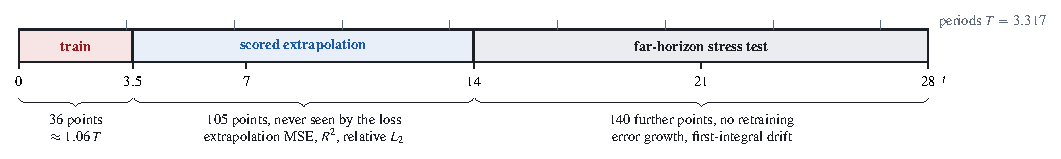
\includegraphics[width=0.85\textwidth]{figures/tikz/data_split.pdf}
\caption{Time axis of the Lotka-Volterra protocol. Tick marks above the bar
are multiples of the true period. The far-horizon window $(14,28]$ is used
only for the stress tests of Sections~\ref{sec:crossdomain}
and~\ref{sec:phase4}; no model is retrained or reselected for it.}
\label{fig:data-split}
\end{figure*}

Writing $\hat{\mathbf{u}}_k$ for the model's prediction and $\mathbf{u}_k$
for the truth at the $N_e=105$ test samples, the reported metrics are
\begin{gather}
\mathrm{MSE}=\frac{1}{2N_e}\sum_{k}\|\hat{\mathbf{u}}_k-\mathbf{u}_k\|_2^2,\qquad
R^2 = 1-\frac{\sum_k\|\hat{\mathbf{u}}_k-\mathbf{u}_k\|_2^2}{\sum_k\|\mathbf{u}_k-\bar{\mathbf{u}}\|_2^2},
\nonumber\\
\text{rel.}\,L_2=\frac{\big(\sum_k\|\hat{\mathbf{u}}_k-\mathbf{u}_k\|_2^2\big)^{1/2}}{\big(\sum_k\|\mathbf{u}_k\|_2^2\big)^{1/2}},
\label{eq:metrics}
\end{gather}
where $\bar{\mathbf{u}}$ is the componentwise mean of the true test
trajectory. $R^2=1$ is a perfect match, $R^2=0$ is no better than
predicting that mean, and a negative value is worse than that trivial
baseline. Two further quantities describe the trained field rather than its
trajectory. The \textbf{Lipschitz estimate}
\begin{equation}
\hat L=\max_{k\le 36}\frac{\|\mathbf{f}_\theta(\mathbf{u}_k+\varepsilon\mathbf{v}_k)-\mathbf{f}_\theta(\mathbf{u}_k)\|_2}{\varepsilon},
\label{eq:lipschitz}
\end{equation}
with $\varepsilon=10^{-3}$ and random unit vectors $\mathbf{v}_k$, is a
finite-difference sample of the local slope of $\mathbf{f}_\theta$ at the
training states. It is a \emph{lower} bound on the field's true Lipschitz
constant and measures how sharply the learned field bends. The
\textbf{cost} of a solver is its number of function evaluations (NFE): an
$s$-stage method on the training window costs $\text{NFE}=35\times2\times
s=70s$ calls of $\mathbf{f}_\theta$ per epoch. Because reverse-mode
differentiation unrolls every call, training wall-clock scales with it too.

\subsection{Computational budget: why 10{,}000 epochs}
\label{sec:budget}

The base paper trains for $10^5$ epochs. Table~\ref{tab:cost} shows what
that would cost us. The paper's integration loop is compiled by Julia's
SciML stack; ours is interpreted PyTorch on CPU, where every Runge-Kutta
stage is a separate Python-level call with its own autograd bookkeeping. On
our development machine one Tsit5/RBF epoch takes $0.17$~s and one
Tsit5/B-spline epoch $0.67$~s; the cloud CPUs we used for the long runs of
Section~\ref{sec:phase4} were $2.2$--$2.5\times$ slower for every KAN
configuration.

\begin{table*}[t]
\centering
\footnotesize
\renewcommand{\arraystretch}{1.1}
\caption{Measured per-epoch cost on our local development CPU and on cloud
(Kaggle) CPU, each averaged over the full run, and the projected cost of the
paper's $10^5$-epoch budget.}
\label{tab:cost}
\begin{tabular}{@{}L{4.2cm} C{1.6cm} C{1.6cm} C{1.2cm} C{2.5cm} C{2.5cm}@{}}
\toprule
\hdrrow \thh{Configuration} & \thh{Local s/epoch} & \thh{Cloud s/epoch} & \thh{Ratio} & \thh{$10^5$ epochs, local} & \thh{$10^5$ epochs, cloud}\\
\midrule
Euler / RBF & $0.0254$ & $0.0627$ & $2.47\times$ & $0.7$ h & $1.7$ h\\
Tsit5 / RBF (reference) & $0.1705$ & $0.4033$ & $2.37\times$ & $4.7$ h & $11.2$ h\\
Tsit5 / B-spline & $0.6680$ & $1.5438$ & $2.31\times$ & $18.6$ h & $42.9$ h\\
MLP-ODE, SiLU $[2,14,8,8,2]$ & $0.2856$ & $0.2722$ & $0.95\times$ & $7.9$ h & $7.6$ h\\
MLP-ODE, tanh $[2,50,2]$ & $0.0736$ & $0.1595$ & $2.17\times$ & $2.0$ h & $4.4$ h\\
\midrule
All 24 Lotka-Volterra configurations & \multicolumn{2}{c}{$14.2$ CPU-h at $10^4$ epochs} & & $142$ h & $\approx336$ h\\
\bottomrule
\end{tabular}
\end{table*}

A $10^5$-epoch version of the 24-configuration Lotka-Volterra sweep would
need roughly $142$ CPU-hours locally, or about two weeks of cloud CPU time,
before the pendulum, SIR and follow-on studies. We therefore ran the sweep
at $10^4$ epochs, a budget at which every noise-free solver and basis
configuration except Euler and four bases (Lagrange, IQF, RSWAF, Newton)
reaches $10^{-4}$ training MSE (Table~\ref{tab:milestones}). That choice is
only safe if the conclusions drawn at $10^4$ epochs survive a longer budget,
which is exactly what Section~\ref{sec:phase4} tests.


\section{Results and Discussion}
\label{sec:results}
We report the studies in the order of Table~\ref{tab:work-summary}. Most
of them open with a short box stating the question, what we expected, and
what we observed, and close with a verdict. Sections~\ref{sec:kan-vs-mlp}
to~\ref{sec:crossdomain} establish the baseline and the ablations,
Sections~\ref{sec:track-a} to~\ref{sec:track-e} are follow-on studies that
each isolate one question, and Section~\ref{sec:phase4} re-tests the
budget-sensitive conclusions at five times the training budget.
Section~\ref{sec:audit} then compares our findings with the base paper, and
Section~\ref{sec:discussion} draws out the patterns that recur across
studies.

\subsection{Baseline reproduction: KAN-ODE vs.\ MLP-ODE}
\label{sec:kan-vs-mlp}

Two MLP vector fields with 252 parameters were trained under the identical
recipe: the paper's literal baseline, one hidden layer of 50 tanh units, and
a deeper $[2,14,8,8,2]$ SiLU network that trains reliably under our
protocol. Table~\ref{tab:kan-vs-mlp} and Figures~\ref{fig:kan-vs-mlp}
and~\ref{fig:kan-vs-mlp-t28} compare
them with the KAN-ODE. A fourth column, added after auditing the paper's own
code (Section~\ref{sec:audit}), retrains the identical literal baseline under
the paper's own learning rate and initialization scale instead of our
default. Figures~\ref{fig:kan-vs-mlp} and~\ref{fig:kan-vs-mlp-t28} plot that run
in place of the default-setting tanh MLP.

\begin{table*}[t]
\centering
\footnotesize
\renewcommand{\arraystretch}{1.12}
\caption{KAN-ODE against parameter-matched MLP-ODEs at $10^4$ epochs.
Epoch counts are the first epoch at which the training loss falls below the
threshold. The last three rows are computed from the saved checkpoints:
field error is $\|\mathbf{f}_\theta-\mathbf{f}\|_2$ averaged over the true
orbit on $(3.5,14]$ and divided by the mean $\|\mathbf{f}\|_2=4.82$ there;
the period is measured from zero-crossings of the predicted prey signal over
$[0,28]$; $H$ drift is $\max_t|H(\hat{\mathbf{u}}(t))-H_0|/H_0$ on $[0,28]$.
The fourth column is the identical literal baseline of the third, retrained
under the paper's own learning rate and initialization scale
(Section~\ref{sec:audit}); its $5\times10^4$-epoch continuation is in
Table~\ref{tab:phase4}.}
\label{tab:kan-vs-mlp}
\begin{tabularx}{\textwidth}{@{}Y C{2.85cm} C{2.85cm} C{2.85cm} C{2.85cm}@{}}
\toprule
\hdrrow \thh{Metric} & \thh{KAN-ODE (RBF)} & \thh{MLP-ODE (SiLU)} & \thh{MLP-ODE (tanh, default lr/init)} & \thh{MLP-ODE (tanh, paper's lr/init)}\\
\midrule
Parameters & 240 & 252 & 252 & 252\\
Training MSE & $8.83\times10^{-5}$ & $9.50\times10^{-5}$ & $1.08\times10^{0}$ & $1.11\times10^{-3}$\\
Extrapolation MSE & $\mathbf{8.92\times10^{-5}}$ & $4.77\times10^{-4}$ & $1.69\times10^{0}$ & $9.65\times10^{-3}$\\
Extrapolation $R^2$ & $\mathbf{0.99997}$ & $0.99984$ & $0.4215$ & $0.99669$\\
Relative $L_2$ error & $\mathbf{0.33\%}$ & $0.76\%$ & $45.2\%$ & $3.42\%$\\
Lipschitz estimate $\hat L$ & $6.91$ & $\mathbf{5.07}$ & $38.22$ & $9.23$\\
Epochs to $10^{-2}$ / $10^{-3}$ / $10^{-4}$ & $3112$ / $5282$ / $9617$ & $\mathbf{741}$ / $\mathbf{1297}$ / $\mathbf{9145}$ & never & $3461$ / never / never\\
Wall-clock, $10^4$ epochs & $1705$ s & $2856$ s & $736$ s & $1052$ s\\
\midrule
Field error on the orbit, $(3.5,14]$ & $2.84\%$ & $2.82\%$ & -- & $7.03\%$\\
Relative period error & $\mathbf{1.7\times10^{-5}}$ & $8.0\times10^{-4}$ & -- & $3.1\times10^{-3}$\\
Max.\ first-integral drift & $3.1\%$ & $\mathbf{2.8\%}$ & -- & $22.7\%$\\
\bottomrule
\end{tabularx}
\end{table*}

\begin{figure}[t]
\centering
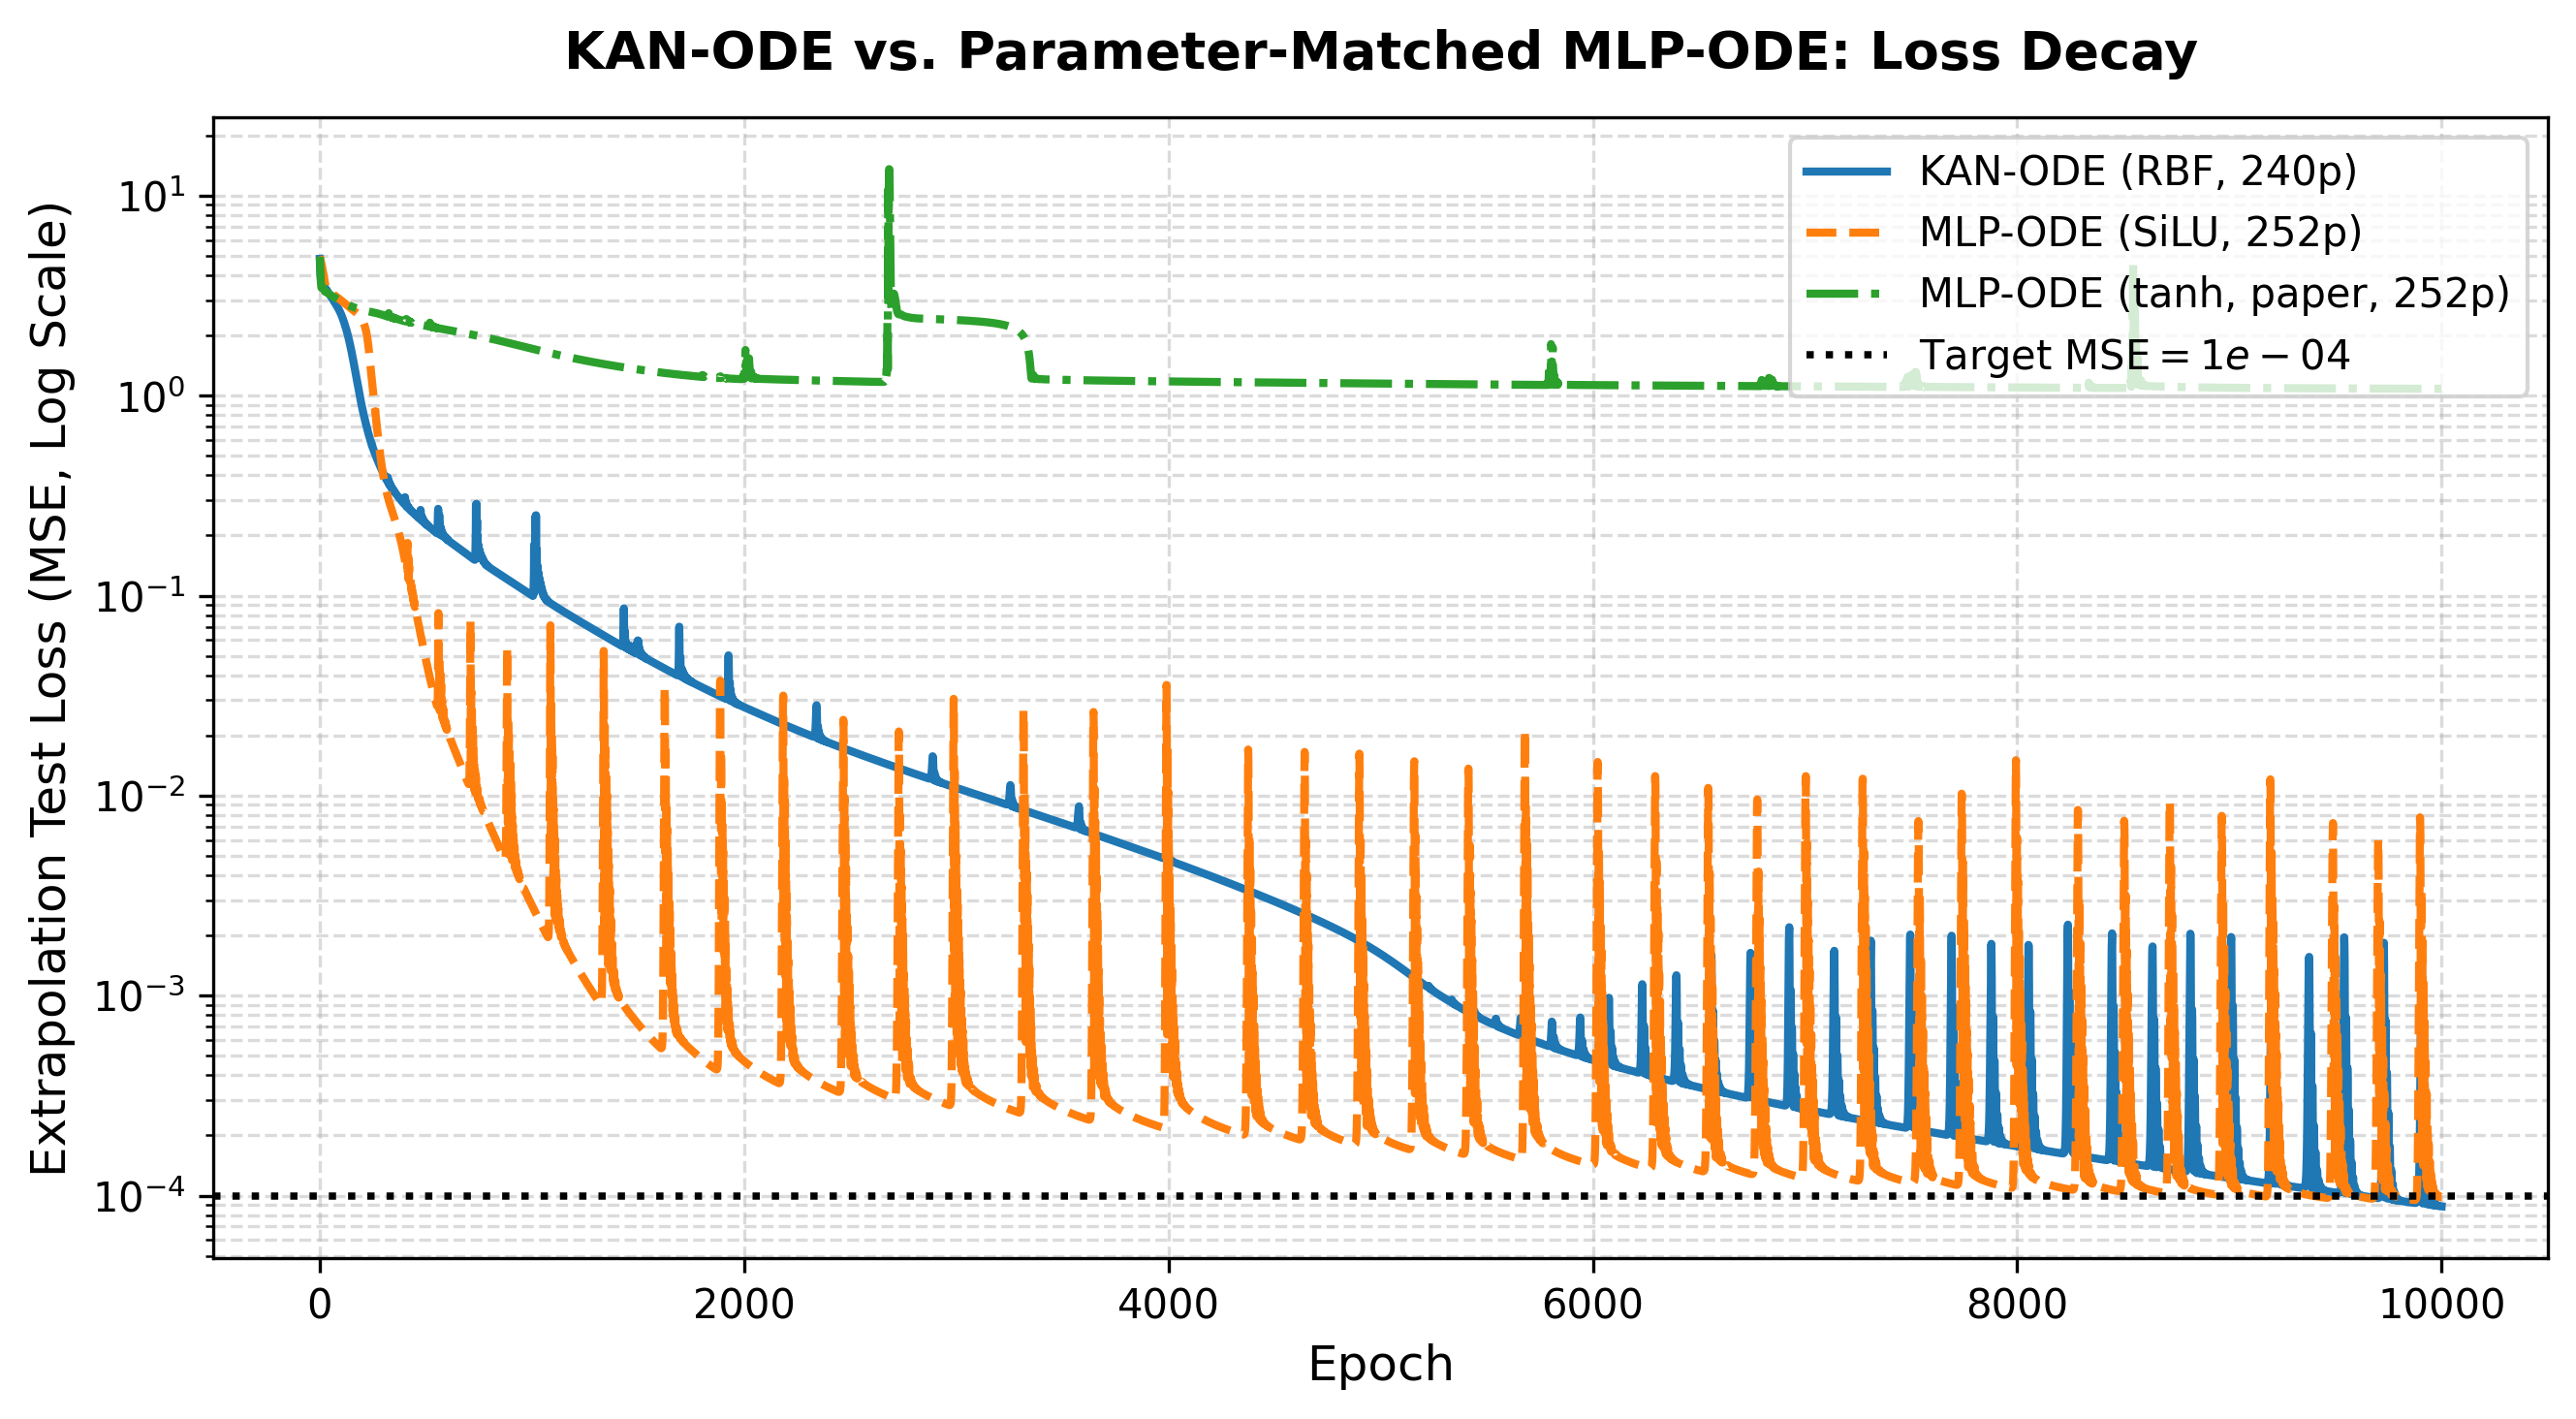
\includegraphics[width=\columnwidth]{figures/ablation/03_kan_vs_mlp_convergence.png}
\caption{Training MSE per epoch for KAN-ODE and the paper's
parameter-matched tanh MLP-ODE, trained with the paper's own learning rate
and initialization (fourth column of Table~\ref{tab:kan-vs-mlp}). KAN-ODE
descends steadily and reaches $10^{-4}$ at epoch 9617; the tanh MLP reaches
$10^{-2}$ at epoch 3461 but never $10^{-3}$ within $10^4$ epochs.}
\label{fig:kan-vs-mlp}
\end{figure}

\begin{figure}[t]
\centering
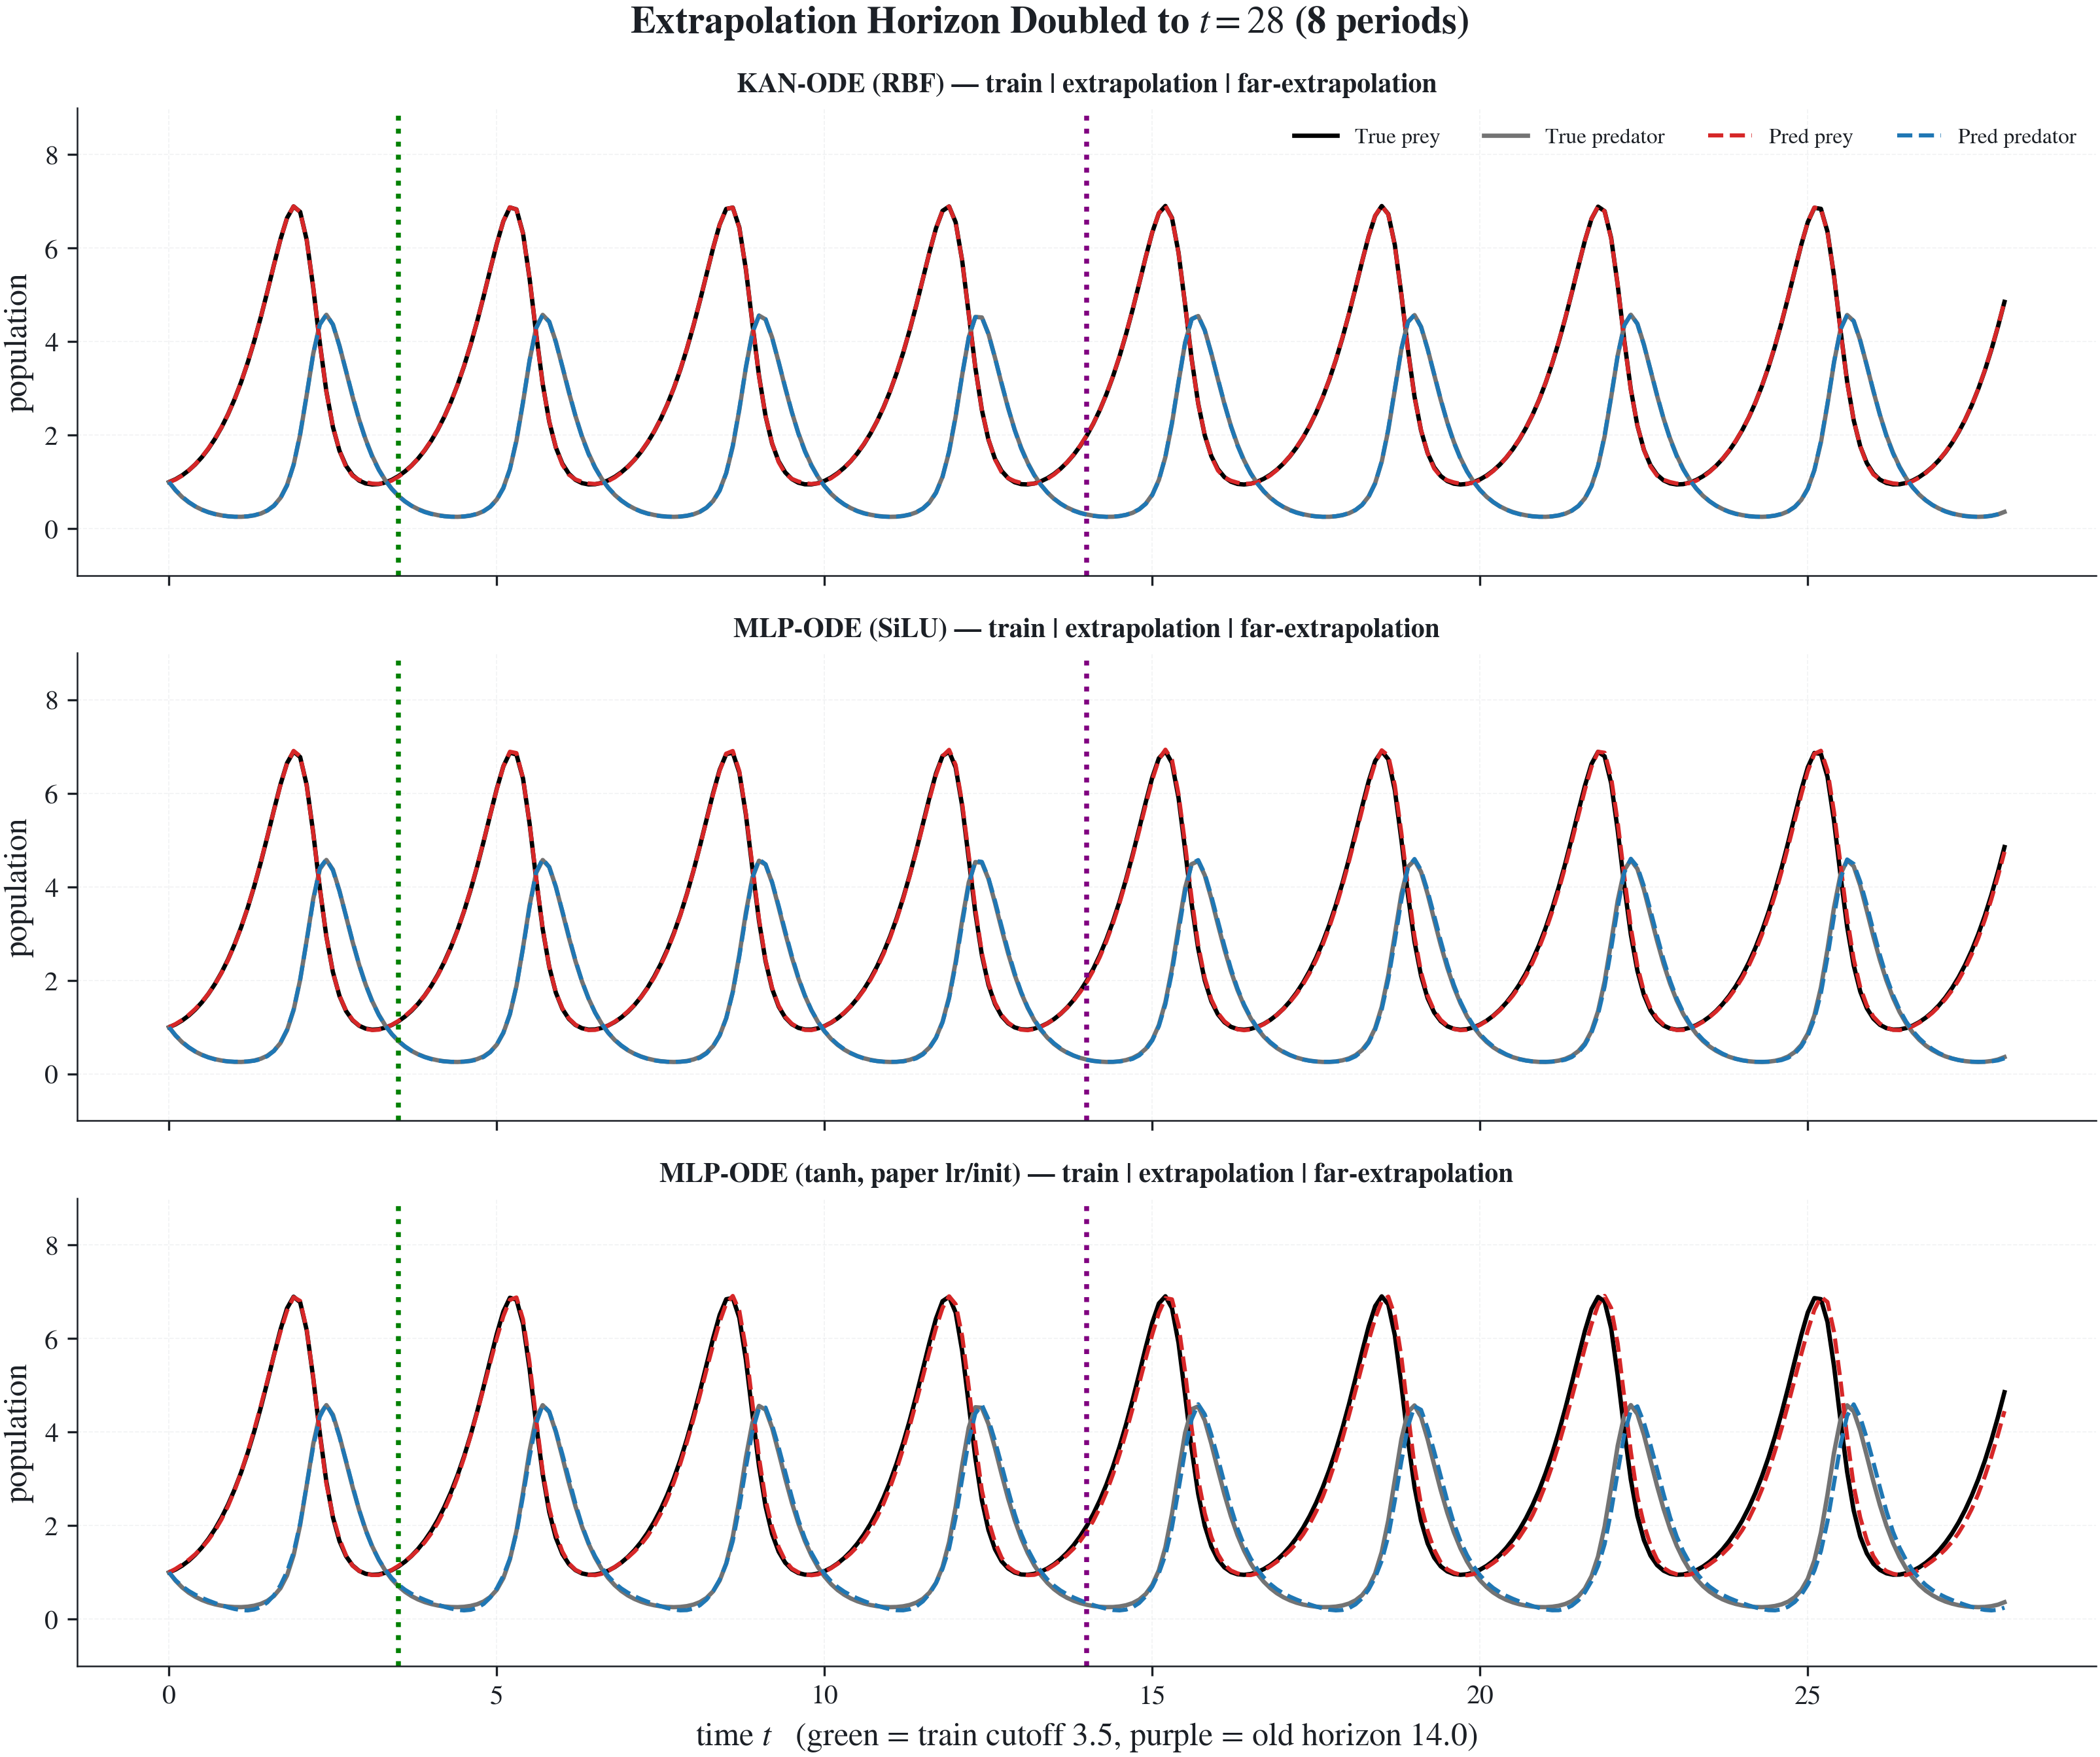
\includegraphics[width=\columnwidth]{figures/ablation/07_extrapolation_t28.png}
\caption{Predicted against true populations out to $t=28$ for the three
models, with no retraining. KAN-ODE and SiLU-MLP are visually
indistinguishable from the truth. The paper's tanh MLP under its own
learning rate and initialization (bottom, fourth column of
Table~\ref{tab:kan-vs-mlp}) follows the training window and the first
periods closely, then runs slightly slow and lags visibly by the far
window $(14,28]$.}
\label{fig:kan-vs-mlp-t28}
\end{figure}

The fourth column shows that the paper's literal architecture was never the
problem. Given the paper's own learning rate and initialization scale, the
identical tanh network reaches $R^2=0.997$. We return to this in
Section~\ref{sec:phase4}, which also reports its $5\times10^4$-epoch
continuation. The next two paragraphs compare KAN-ODE against the working
SiLU baseline, columns one and two.

We find one result that confirms the paper and one that contradicts it.
\textbf{KAN-ODE extrapolates $5.4\times$ better} from a training loss only
$7\%$ lower, reproducing the paper's accuracy claim. The checkpoints show
where that gap comes from. Both fields are equally accurate on the orbit
($2.84\%$ against $2.82\%$ mean field error), and both hold the invariant
to about $3\%$, but the MLP's orbit period is off by $8.0\times10^{-4}$
against the KAN's $1.7\times10^{-5}$, a $48\times$ larger period error. On a
periodic orbit a period error $\epsilon_T$ becomes a phase lag that grows
linearly, $\approx 2\pi\epsilon_T\, t/T$, so the trajectory error of the MLP
keeps accumulating while the KAN's stays near its training-window level.
The extrapolation gap is a phase-accuracy gap rather than a field-accuracy
gap. \textbf{The MLP converges faster, not slower}: it reaches $10^{-3}$
training MSE at epoch 1297 against the KAN's 5282, $4.1\times$ sooner. This
contradicts the paper's headline efficiency claim on this same system (a
$10^4$-epoch KAN-ODE against a $10^5$-epoch MLP-ODE). Under our protocol, at
matched parameter count and optimizer settings, the MLP was the faster model
to train; KAN-ODE won on extrapolation, the paper's other headline claim.

\paragraph{Why the paper's literal MLP fails to train under our default
optimizer settings.} The $[2,50,2]$ tanh network never gets below a
training MSE of $1.08$ at our default learning rate
($2\times10^{-3}$) and initialization (Glorot, gain $1.0$). A controlled
2000-epoch factorial run, holding those optimizer settings fixed, separates
the two things that differ between it and the working baseline
(Table~\ref{tab:mlp-breakdown}).

\begin{table*}[t]
\centering
\footnotesize
\renewcommand{\arraystretch}{1.15}
\caption{Controlled breakdown of why the paper's literal MLP baseline
architecture, $[2,50,2]$ with hyperbolic tangent (tanh) activation, fails to
train at our default learning rate and initialization scale. All
four runs use 2000 epochs and Glorot initialization at gain $1.0$; none
varies the initialization scale (see the paragraph following this table).}
\label{tab:mlp-breakdown}
\begin{tabularx}{\textwidth}{@{}C{0.9cm} Y C{1.8cm} C{2.0cm} C{2.6cm} C{2.6cm} C{2.0cm}@{}}
\toprule
\hdrrow \thh{Run} & \thh{Architecture} & \thh{Activation} & \thh{Learning rate} & \thh{Training MSE} & \thh{Extrapolation MSE} & \thh{$R^2$}\\
\midrule
A & $[2,50,2]$ & tanh & $2\times10^{-3}$ & $1.21\times10^{0}$ & $1.98\times10^{0}$ & $0.319$\\
B & $[2,50,2]$ & tanh & $5\times10^{-4}$ & $1.85\times10^{0}$ & $9.23\times10^{0}$ & $-2.169$\\
C & $[2,14,8,8,2]$ & SiLU & $2\times10^{-3}$ & $\mathbf{4.28\times10^{-4}}$ & $\mathbf{6.97\times10^{-4}}$ & $\mathbf{0.99976}$\\
D & $[2,50,2]$ & SiLU & $2\times10^{-3}$ & $3.62\times10^{-3}$ & $2.68\times10^{2}$ & $-91.06$\\
\bottomrule
\end{tabularx}
\end{table*}

Runs A and D share the architecture and differ only in activation. The
training MSE falls from $1.21$ to $3.62\times10^{-3}$, a $335\times$
improvement, so at these optimizer settings, activation decides whether this
architecture fits the data at all. Runs C and D share the SiLU activation and
differ only in depth. The shallow network fits the window but its
extrapolation error explodes to $2.68\times10^{2}$, against
$6.97\times10^{-4}$ for the deep one, so depth decides whether a model that
trains also extrapolates. Lowering the learning rate alone (run B) makes the
tanh network worse, not better. Five times the epoch budget under these
same settings does not rescue it either: at $5\times10^4$ epochs, training
MSE moves only from $1.08$ to $1.01$ and extrapolation gets \emph{worse}
(Table~\ref{tab:phase4}).

\paragraph{The actual cause: learning rate and initialization scale, not
architecture.} None of runs A--D varies the initialization scale, and the
base paper's own published code turned out to use a combination this
factorial never tested: a learning rate of $10^{-2}$ (five times our
default) together with weights initialized near zero (Glorot
divided by $10^5$), for the identical $[2,50,2]$ tanh architecture. Retrained
with only those two settings changed, the literal architecture trains
(Table~\ref{tab:kan-vs-mlp}, fourth column). At $10^4$ epochs it reaches a
training MSE of $1.11\times10^{-3}$ (against $1.08$ before) and an
extrapolation MSE of $9.65\times10^{-3}$, $R^2=0.997$ (against $R^2=0.42$
before), with a Lipschitz estimate of $9.23$ against $38.2$. At $5\times10^4$
epochs it reaches $5.43\times10^{-5}$ training MSE
and $R^2=0.9998$ on extrapolation, with zero non-finite gradient steps and no
clipping in either run. Section~\ref{sec:phase4} reports the full comparison
against KAN-ODE and the SiLU MLP at both budgets, and updates the
implementation audit accordingly. The paper's literal recipe was never
architecturally incompatible with this system. Our default
optimizer settings, tuned around the KAN-ODE side of the comparison, were the
wrong settings for a wide, near-linear-at-initialization tanh network, and
Table~\ref{tab:mlp-breakdown}'s factorial measured sensitivity to activation
\emph{at those settings} rather than an architecture-level limit.

\subsection{Integrator ablation}
\label{sec:solver-results}

We first verify that each integrator of Section~\ref{sec:integrators} is the
method it claims to be, then sweep all six at a fixed RBF basis.

\subsubsection{Order verification and linear stability}

\paragraph{Verifying the implementations.} Two independent checks confirm
that each integrator is the method it claims to be. The first is the order
conditions: a Runge-Kutta method has order $p$ exactly when
$\mathbf{b}^\top\Phi(\tau)=1/\gamma(\tau)$ for every rooted tree $\tau$ with at most
$p$ vertices, where $\Phi(\tau)$ is the tree's elementary weight built from
$A$ and $\gamma(\tau)$ its density \cite{hairer1993solving}. We enumerate all
37 rooted trees up to six vertices and evaluate each condition directly on
the implemented coefficients. This gives the verified order and the principal
error norm $A^{(p+1)}=\big(\sum_{|\tau|=p+1}\big[(\mathbf{b}^\top\Phi(\tau)-1/\gamma(\tau))/\sigma(\tau)\big]^2\big)^{1/2}$,
the size of the leading local-error term. The second is a work-precision study on
the \emph{true} Lotka-Volterra field: integrating from $(1,1)$ to $t=3.5$ at
eight step sizes and comparing against the DOP853 reference gives the
observed order $\hat p$ as the slope of $\log\|\text{error}\|$ against
$\log h$ (Figure~\ref{fig:work-precision}). Table~\ref{tab:order-conditions}
collects both.

\begin{table*}[t]
\centering
\footnotesize
\renewcommand{\arraystretch}{1.12}
\caption{Order verification of the implemented integrators. ``Max residual''
is the largest $|\mathbf{b}^\top\Phi(\tau)-1/\gamma(\tau)|$ over all trees up
to the design order ($1+1+2+4+9=17$ conditions at order five);
$A^{(p+1)}$ is the principal error norm; $\hat p$ is the slope fitted to
the work-precision data for $h\le0.1$ above the round-off floor.}
\label{tab:order-conditions}
\begin{tabularx}{\textwidth}{@{}Y C{1.4cm} C{1.8cm} C{2.0cm} C{3.0cm} C{2.3cm} C{2.0cm}@{}}
\toprule
\hdrrow \thh{Method} & \thh{Stages $s$} & \thh{Verified order $p$} & \thh{Conditions checked} & \thh{Max residual through order $p$} & \thh{$A^{(p+1)}$} & \thh{Observed $\hat p$}\\
\midrule
Forward Euler & 1 & 1 & 1 & $0$ & $5.00\times10^{-1}$ & $1.00$\\
Heun & 2 & 2 & 2 & $0$ & $1.86\times10^{-1}$ & $2.10$\\
Midpoint & 2 & 2 & 2 & $0$ & $1.72\times10^{-1}$ & $2.07$\\
Classical RK4 & 4 & 4 & 8 & $1.1\times10^{-16}$ & $1.45\times10^{-2}$ & $3.93$\\
DOPRI5 (6 of 7) & 6 & 5 & 17 & $2.8\times10^{-16}$ & $3.99\times10^{-4}$ & $5.66$\\
Tsit5 (6 of 7) & 6 & 5 & 17 & $1.4\times10^{-14}$ & $\mathbf{1.39\times10^{-4}}$ & $5.95$\\
\bottomrule
\end{tabularx}
\end{table*}

\begin{figure*}[t]
\centering
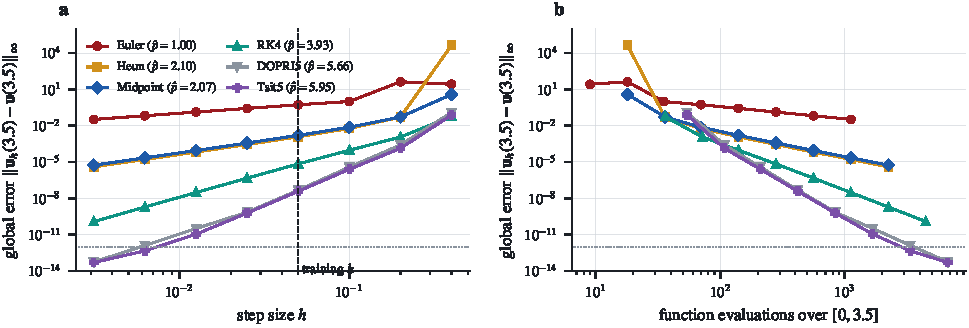
\includegraphics[width=\textwidth]{figures/analysis/work_precision.pdf}
\caption{Global error at $t=3.5$ of each implemented integrator applied to the
true Lotka-Volterra field. (a) Against step size, with fitted slopes;
the dashed line is the training step $h=0.05$. (b) Against the number of
field evaluations, the quantity that sets training cost. At $h=0.4$ both
second-order methods blow up,
and the fifth-order methods reach the round-off floor near $10^{-13}$.}
\label{fig:work-precision}
\end{figure*}

Every method satisfies its order conditions to round-off and shows its
design order in practice. The fifth-order pair shows slightly super-nominal
slopes over this range because its error is still pre-asymptotic before it
hits round-off. The principal error norms confirm Tsitouras's design goal
from the code's own coefficients: Tsit5's leading error term is
$2.9\times$ smaller than DOPRI5's. The table also sets up a point used
below. Heun and Midpoint differ only in their third-order error terms, and
on those Midpoint's is marginally \emph{smaller} ($0.172$ against $0.186$).

\paragraph{Linear stability.} Applied to $\dot u=\lambda u$, every explicit
Runge-Kutta method multiplies the state by the stability polynomial
$R(z)=1+z\,\mathbf{b}^\top(I-zA)^{-1}\mathbf{1}$, $z=h\lambda$, per step.
Heun and Midpoint share $R(z)=1+z+z^2/2$, so they are indistinguishable on
any linear problem. Figure~\ref{fig:stability}a draws the boundaries
$|R(z)|=1$ and overlays $h\lambda$ for the eigenvalues of the true Jacobian
and of the trained Tsit5 KAN's Jacobian $J_\theta=\partial\mathbf{f}_\theta/\partial\mathbf{u}$,
evaluated at all 141 states of the orbit. The learned eigenvalues track the
true ones closely ($\max|\lambda|=3.61$ against $3.83$), and at $h=0.05$
every $h\lambda$ lies within $0.19$ of the origin, far inside every region.
Stability in the classical sense is therefore never at issue at the training
step. What differs between methods is how accurately $R$ reproduces
$e^{z}$ near the origin. For a purely oscillatory mode $z=i\omega h$,
Figure~\ref{fig:stability}b plots the per-step amplitude error
$|R(i\omega h)|-1$. At Lotka-Volterra's linear frequency
$\omega_0=\sqrt{\alpha\gamma}$, a linear oscillation integrated over one
period gains $39\%$ amplitude under Euler and $0.094\%$ under either
second-order method, and loses $5.8\times10^{-7}$, $2.3\times10^{-8}$ and
$3.5\times10^{-9}$ under RK4, DOPRI5 and Tsit5.

\begin{figure*}[t]
\centering
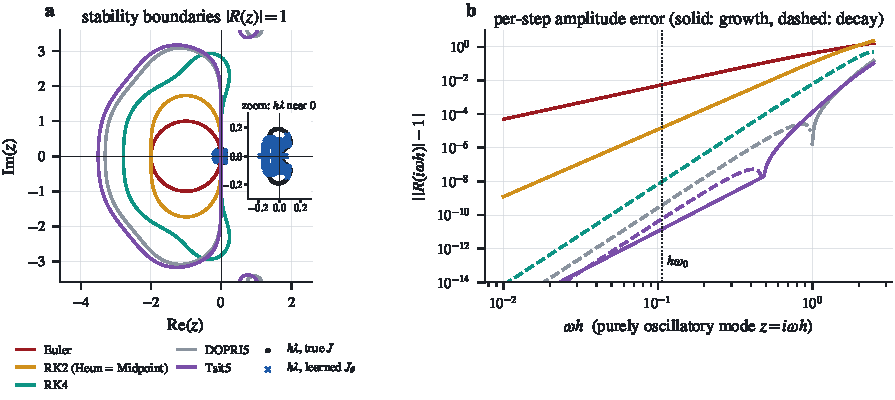
\includegraphics[width=0.85\textwidth]{figures/analysis/stability_regions.pdf}
\caption{(a) Stability boundaries $|R(z)|=1$ computed from each implemented
tableau, with $h\lambda$ for the true Jacobian (dots) and the learned
Jacobian of the Tsit5-trained KAN (crosses) at every state on the orbit,
$h=0.05$; the inset enlarges the neighbourhood of the origin. (b) Per-step
amplitude error for an undamped oscillation; the dotted line marks
$h\omega_0$ at the training step.}
\label{fig:stability}
\end{figure*}

The linear picture is borne out on the true nonlinear field. Integrating the
exact Lotka-Volterra field at the training discretisation and scoring it with
the same extrapolation metric as the trained models isolates each solver's
own truncation error (last column of Table~\ref{tab:solver-ablation}). It is
$17.6$ for Euler, whose trajectory leaves the positive quadrant at
$t=19.4$, $1.3$--$3.0\times10^{-4}$ for the second-order pair, and below
$5\times10^{-9}$ for the rest. The first integral of
Equation~\ref{eq:lv-invariant} tells the same story
(Figure~\ref{fig:first-integral}a): by $t=28$ it has drifted by
$7.5\times10^{-4}$ and $4.5\times10^{-4}$ (relative) under Heun and
Midpoint, $3.0\times10^{-5}$ under RK4, and about $10^{-7}$ under the
fifth-order pair.

\subsubsection{Solver ablation}

Table~\ref{tab:solver-ablation} sweeps the six integrators at fixed RBF
basis; Table~\ref{tab:basis-ablation} in Section~\ref{sec:basis-results}
sweeps seven basis representations at fixed Tsit5 solver. Both use the
protocol of Section~\ref{sec:protocol}. We report the Lipschitz estimate of
the trained field (Equation~\ref{eq:lipschitz}) alongside accuracy because it
measures how smooth or jagged the basis expansion in
Equation~\ref{eq:kan-edge} ended up, independent of the trajectory error.

\begin{table*}[t]
\centering
\footnotesize
\renewcommand{\arraystretch}{1.1}
\caption{Solver ablation (fixed RBF basis, $h=0.05$, 240 parameters,
$10^4$ epochs). The last column integrates the \emph{true} field with the
same solver and step and scores it identically: the solver's own
truncation error, with no learning involved.}
\label{tab:solver-ablation}
\begin{tabularx}{\textwidth}{@{}Y C{1.0cm} C{1.2cm} C{1.9cm} C{1.9cm} C{1.5cm} C{0.9cm} C{1.4cm} C{2.4cm}@{}}
\toprule
\hdrrow \thh{Solver} & \thh{Order} & \thh{NFE / epoch} & \thh{Training MSE} & \thh{Extrap.\ MSE} & \thh{Extrap.\ $R^2$} & \thh{$\hat L$} & \thh{Wall-clock} & \thh{True-field truncation MSE}\\
\midrule
Forward Euler & 1 & 70 & $1.38\times10^{-4}$ & $2.51\times10^{-3}$ & $0.99914$ & $8.55$ & 254 s & $1.8\times10^{1}$\\
Heun RK2 & 2 & 140 & $8.32\times10^{-5}$ & $3.10\times10^{-4}$ & $0.99989$ & $7.07$ & 499 s & $1.3\times10^{-4}$\\
Midpoint & 2 & 140 & $8.86\times10^{-5}$ & $8.95\times10^{-5}$ & $0.99997$ & $6.96$ & \textbf{498 s} & $3.0\times10^{-4}$\\
Classical RK4 & 4 & 280 & $9.41\times10^{-5}$ & $9.29\times10^{-5}$ & $0.99997$ & $6.88$ & 1019 s & $4.7\times10^{-9}$\\
DOPRI5 & 5 & 420 & $9.28\times10^{-5}$ & $9.21\times10^{-5}$ & $0.99997$ & $6.89$ & 1699 s & $6.7\times10^{-14}$\\
\textbf{Tsit5} & 5 & 420 & $\mathbf{8.83\times10^{-5}}$ & $\mathbf{8.92\times10^{-5}}$ & $\mathbf{0.99997}$ & $6.91$ & 1712 s & $4.7\times10^{-14}$\\
\bottomrule
\end{tabularx}
\end{table*}

Truncation error dominates only at order $p=1$. Euler's extrapolation MSE is
$28\times$ Tsit5's, and it is the only solver that fails to reach $10^{-4}$
training loss within budget. Its trained field is also the least smooth of
the six ($\hat L=8.55$, the highest in the table), consistent with a
systematic bias forcing the network to fit a sharper correction than the
smoother integrators require. Above order 2 the ranking collapses into a
$3.8\%$ spread with no monotonic order dependence: at $h=0.05$,
integrator truncation error has fallen below the optimization noise floor.
Midpoint matches Tsit5's accuracy within $0.3\%$ at one third of the
function evaluations and $29\%$ of the wall-clock, making it the
cost-normalized optimum on this problem.

The last column is the striking one. Integrated with the \emph{true} field,
Euler's own error on the extrapolation window is $17.6$. The Euler-trained
network, integrated with Euler, scores $2.5\times10^{-3}$, nearly four orders
of magnitude better than the exact field under the same solver. The same
holds, more mildly, for Midpoint, whose trained model ($8.95\times10^{-5}$)
beats the exact field under Midpoint ($3.0\times10^{-4}$). The network is
not learning $\mathbf{f}$; it is learning whatever field makes
\emph{this solver's} output match the data. Two experiments make that
precise.

\paragraph{The Euler model learns the inverse modified equation.} Backward
error analysis states that Forward Euler applied to a field $\mathbf{g}$
follows, to second order, the modified field
$\mathbf{g}-\tfrac{h}{2}J_{\mathbf{g}}\mathbf{g}+O(h^2)$. For Euler's output
to reproduce the exact flow, the network must therefore learn
\begin{equation}
\mathbf{g}_h=\mathbf{f}+\tfrac{h}{2}\,J_{\mathbf{f}}\,\mathbf{f}+O(h^2).
\label{eq:inverse-modified}
\end{equation}
On the 36 training states, the Euler-trained field differs from the true
field by $9.6\%$ (relative $L_2$), almost exactly the size of the predicted
correction $\tfrac{h}{2}J_{\mathbf{f}}\mathbf{f}$ ($9.2\%$). The learned
correction $\mathbf{f}_\theta-\mathbf{f}$ and the predicted one point the
same way (cosine similarity $0.92$) with a magnitude ratio of $1.04$. Measured
against $\mathbf{g}_h$ instead of $\mathbf{f}$, the Euler model's error falls
to $3.8\%$, comparable to the $3.0\%$ field error of the Tsit5-trained
model. The Euler model is an accurate model of Equation~\ref{eq:inverse-modified}.

\paragraph{Cross-solver transfer.} If each model has absorbed its solver's
error, it should degrade when integrated with a different solver.
Figure~\ref{fig:cross-solver} evaluates every trained model under every
integrator. The Euler model is $70\times$ worse under any other solver
($0.17$--$0.18$), and every other model is $1000$--$7200\times$ worse under
Euler. The second-order models lose $9$--$17\times$ when integrated with a
fourth- or fifth-order method, and the fourth- and fifth-order models lose
$14$--$17\times$ under a second-order one. Within each family the models are
interchangeable: RK4, DOPRI5 and Tsit5 models agree to three significant
figures under all three high-order solvers, so these three have learned
fields that coincide up to their $O(h^4)$ differences. The practical rule is
that a KAN-ODE trained with a low-order solver must be deployed with that
same solver. A trained field is a statement about the physics only
once the training solver's truncation error is below the model error.

\begin{figure}[t]
\centering
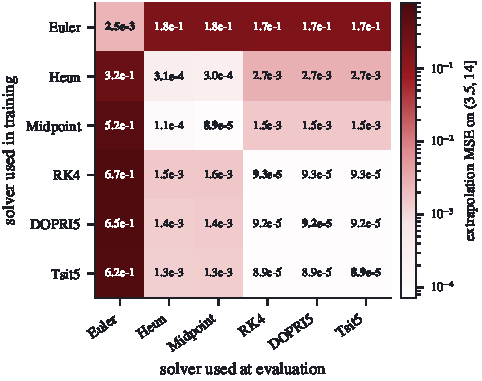
\includegraphics[width=\columnwidth]{figures/analysis/cross_solver_transfer.pdf}
\caption{Extrapolation MSE of each trained model (rows) integrated with
each solver (columns), $h=0.05$. The diagonal (bold) is the configuration
it was trained in.}
\label{fig:cross-solver}
\end{figure}

\begin{figure}[t]
\centering
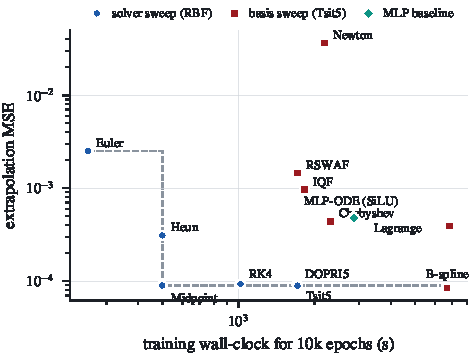
\includegraphics[width=\columnwidth]{figures/analysis/pareto_cost_accuracy.pdf}
\caption{Training wall-clock against extrapolation MSE for the solver and
basis sweeps. The dashed step is the Pareto front: Euler, Midpoint, Tsit5
and B-spline. Midpoint dominates RK4 and DOPRI5 outright.}
\label{fig:pareto}
\end{figure}

\paragraph{Midpoint against Heun.} Midpoint extrapolates $3.5\times$ better
than Heun at identical cost and order. A tempting explanation is that
Heun's end-of-step sampling adds numerical damping. The numbers above rule
that out. The two methods have the same stability polynomial, so they damp
identically on linear modes; Heun is actually the \emph{more} accurate
integrator of the true field ($1.3\times10^{-4}$ against
$3.0\times10^{-4}$ truncation MSE); and the third-order error norms differ
by only $8\%$. The gap belongs to the trained models, not to the
integrators. It shows up as phase accuracy: the Heun model's orbit period is
off by $4.7\times10^{-4}$ (relative), the Midpoint model's by
$3.5\times10^{-6}$ (Table~\ref{tab:equilibria}), and its error envelope grows
ten times faster over $(3.5,28]$ ($5.9\times10^{-3}$ against
$5.7\times10^{-4}$ per unit time). With a single seed per configuration
this ordering could still be an initialisation effect; the solver-level
explanation is refuted either way.

\begin{figure*}[t]
\centering
\begin{subfigure}[b]{0.3\textwidth}
  \centering
  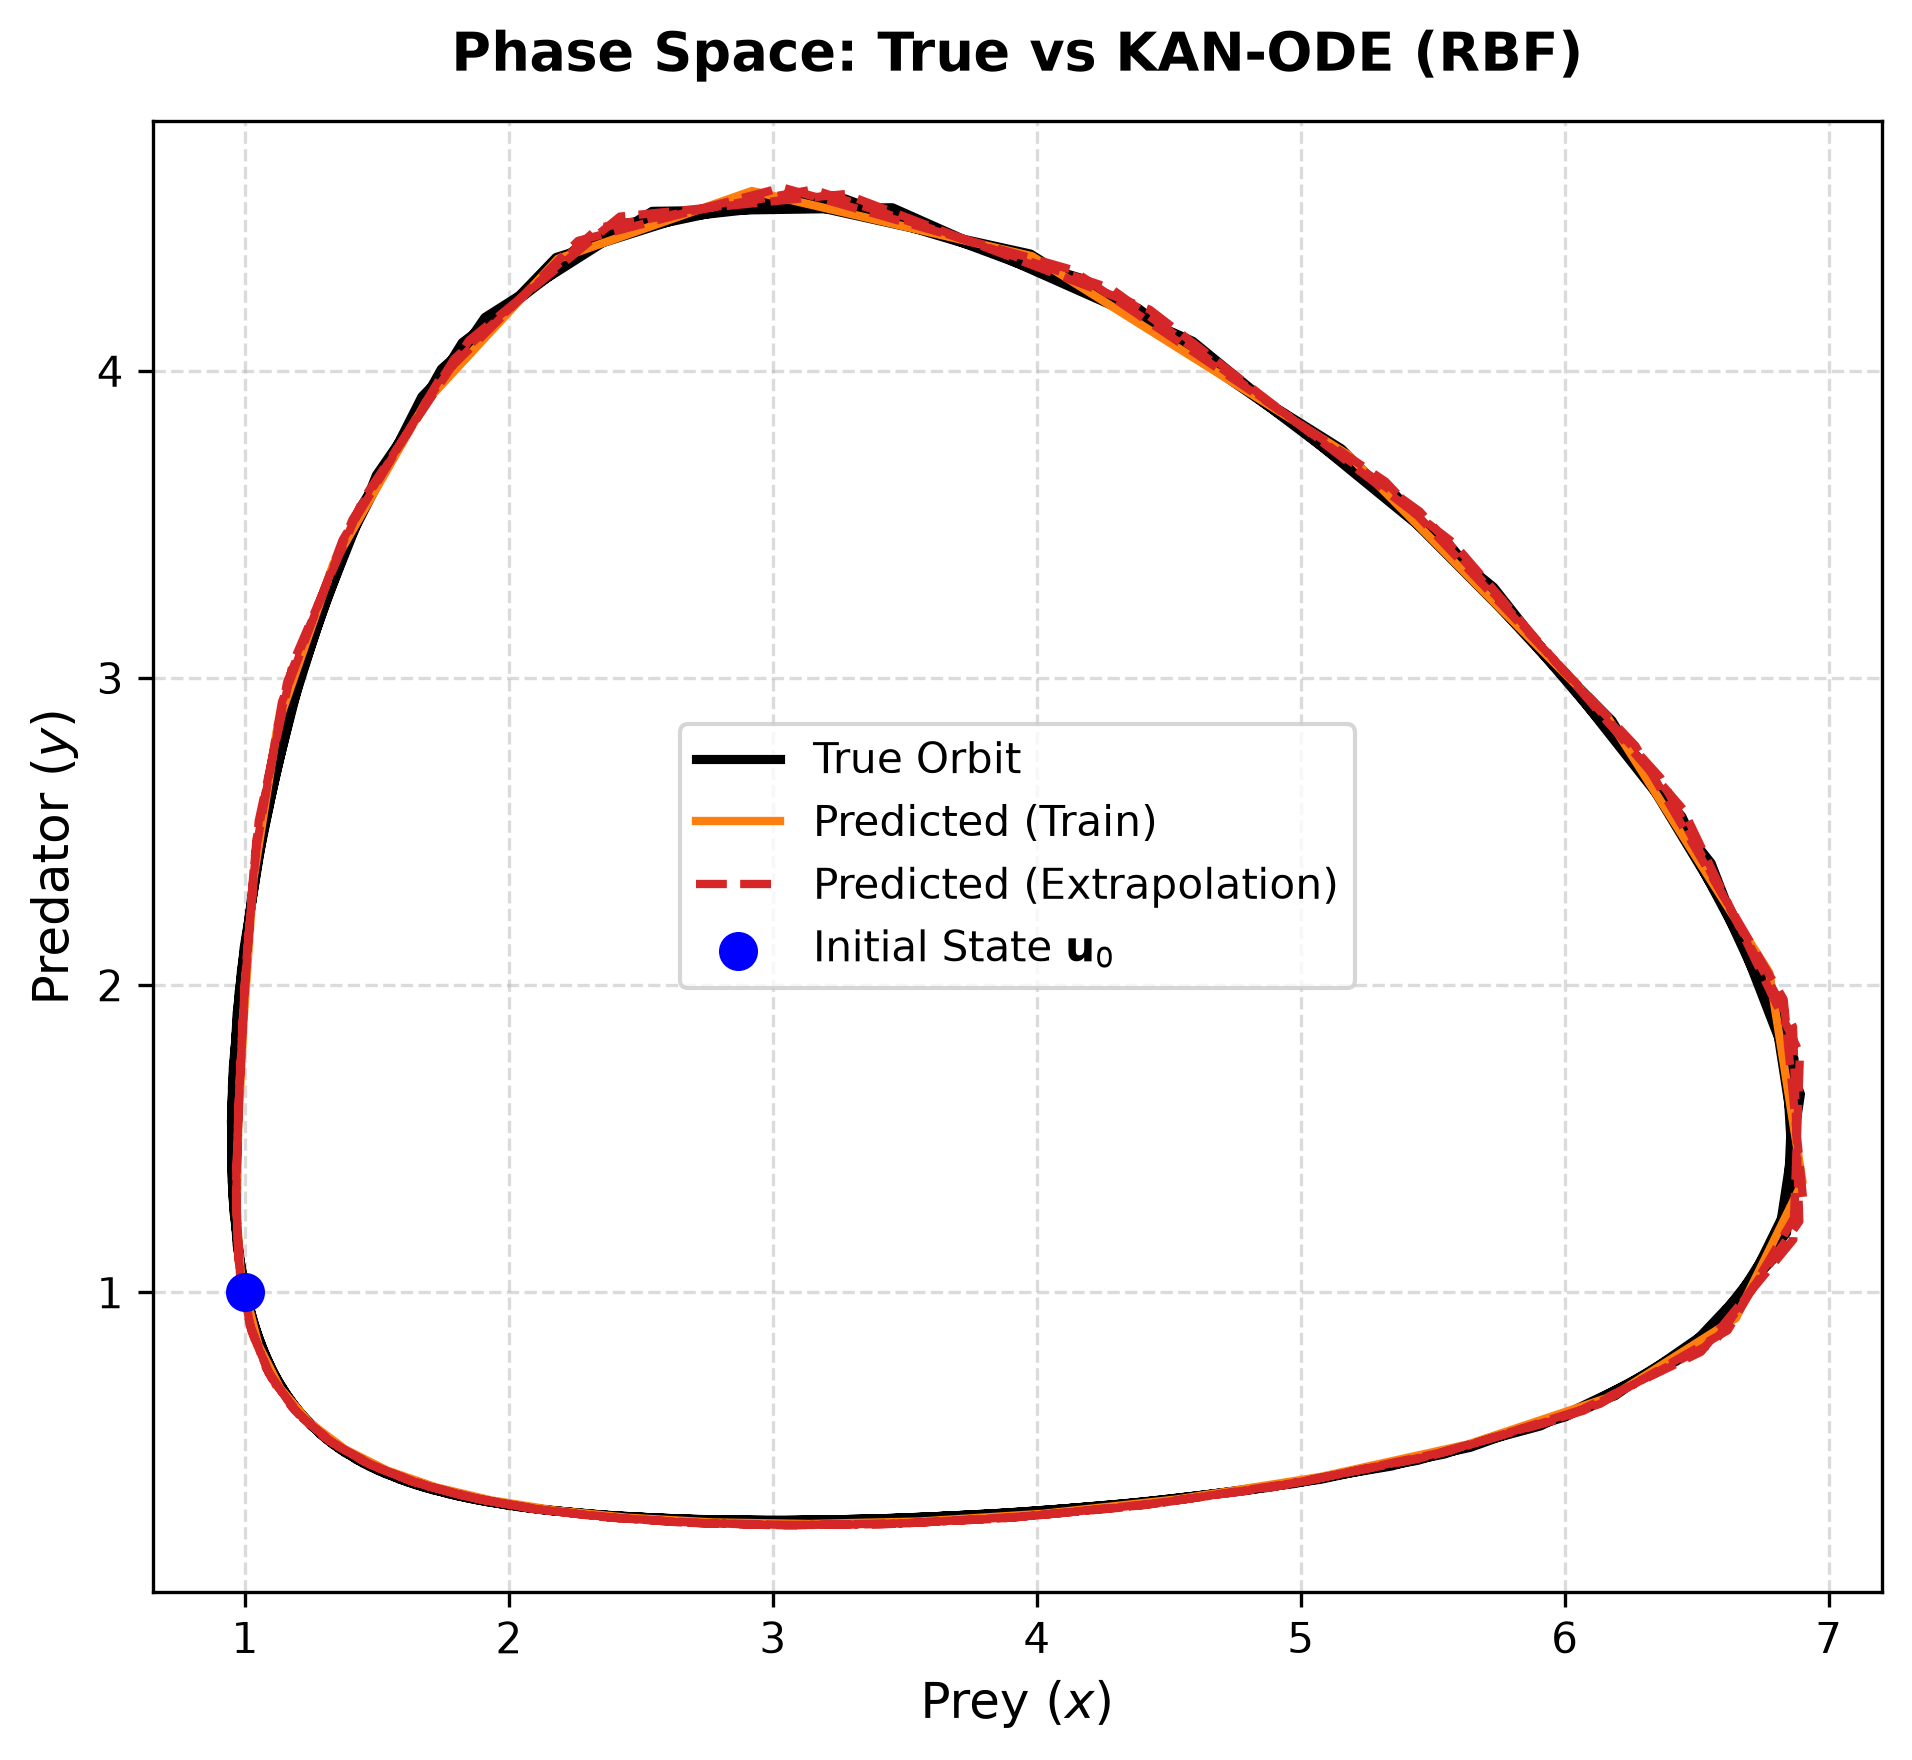
\includegraphics[width=\linewidth]{figures/ablation/solver_euler_phase.png}
  \caption{Forward Euler ($p=1$)}
\end{subfigure}\hfill
\begin{subfigure}[b]{0.3\textwidth}
  \centering
  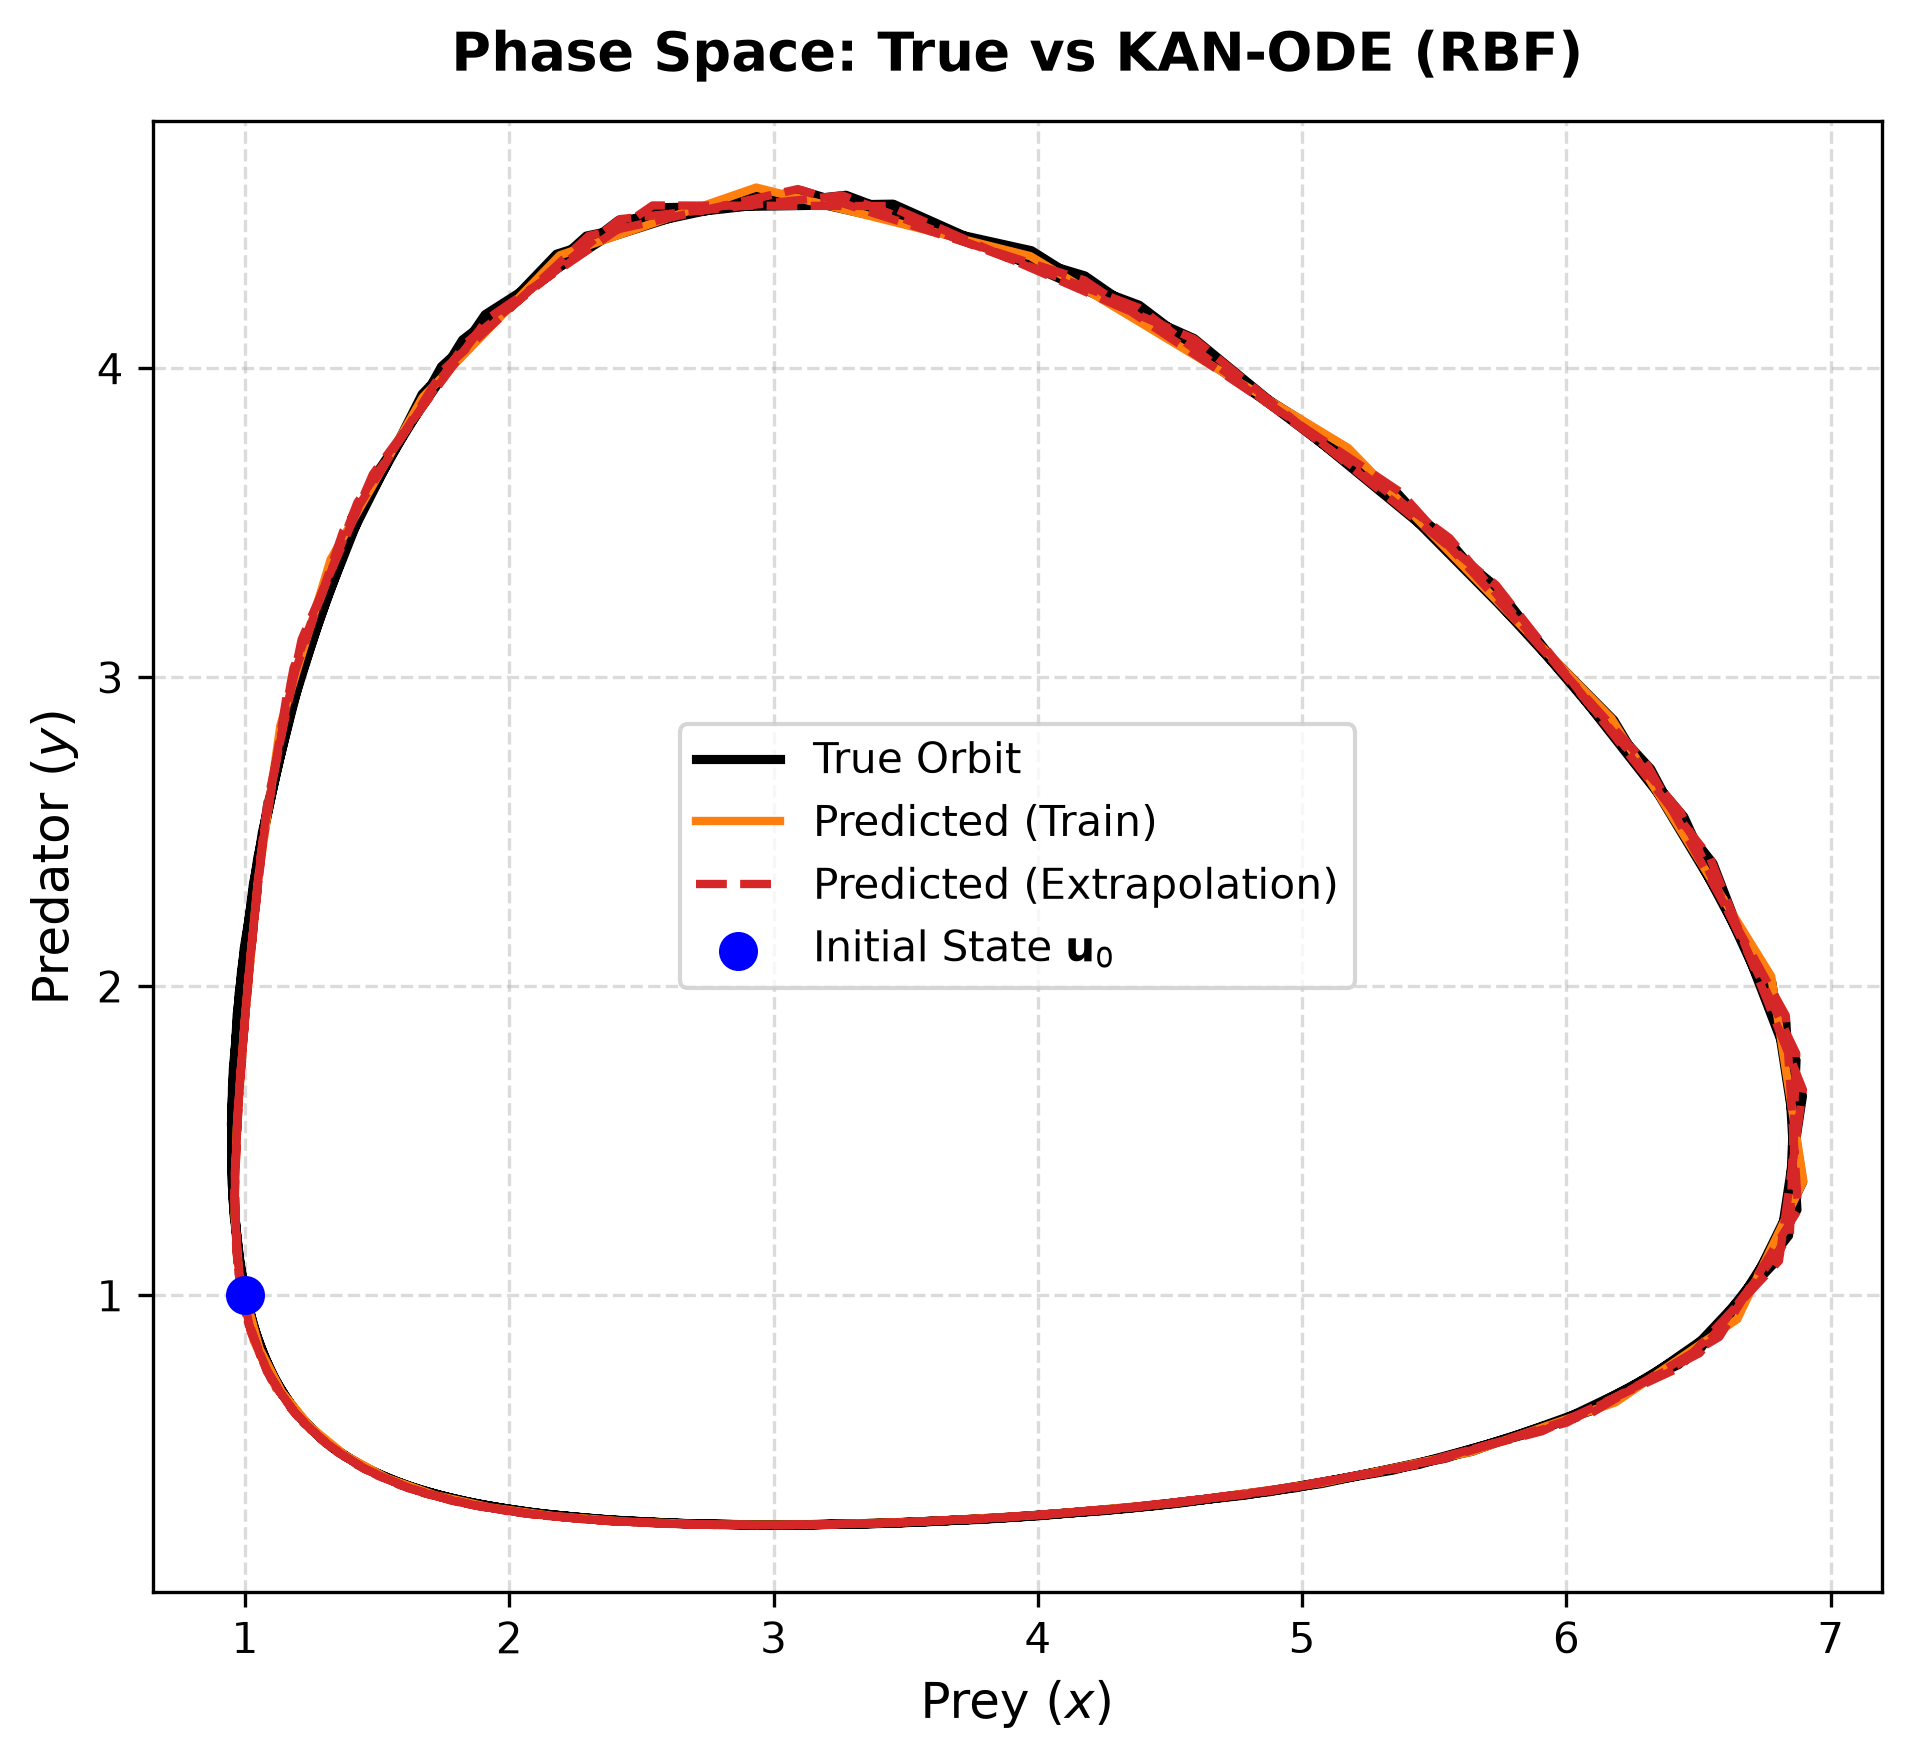
\includegraphics[width=\linewidth]{figures/ablation/solver_midpoint_phase.png}
  \caption{Midpoint ($p=2$)}
\end{subfigure}\hfill
\begin{subfigure}[b]{0.3\textwidth}
  \centering
  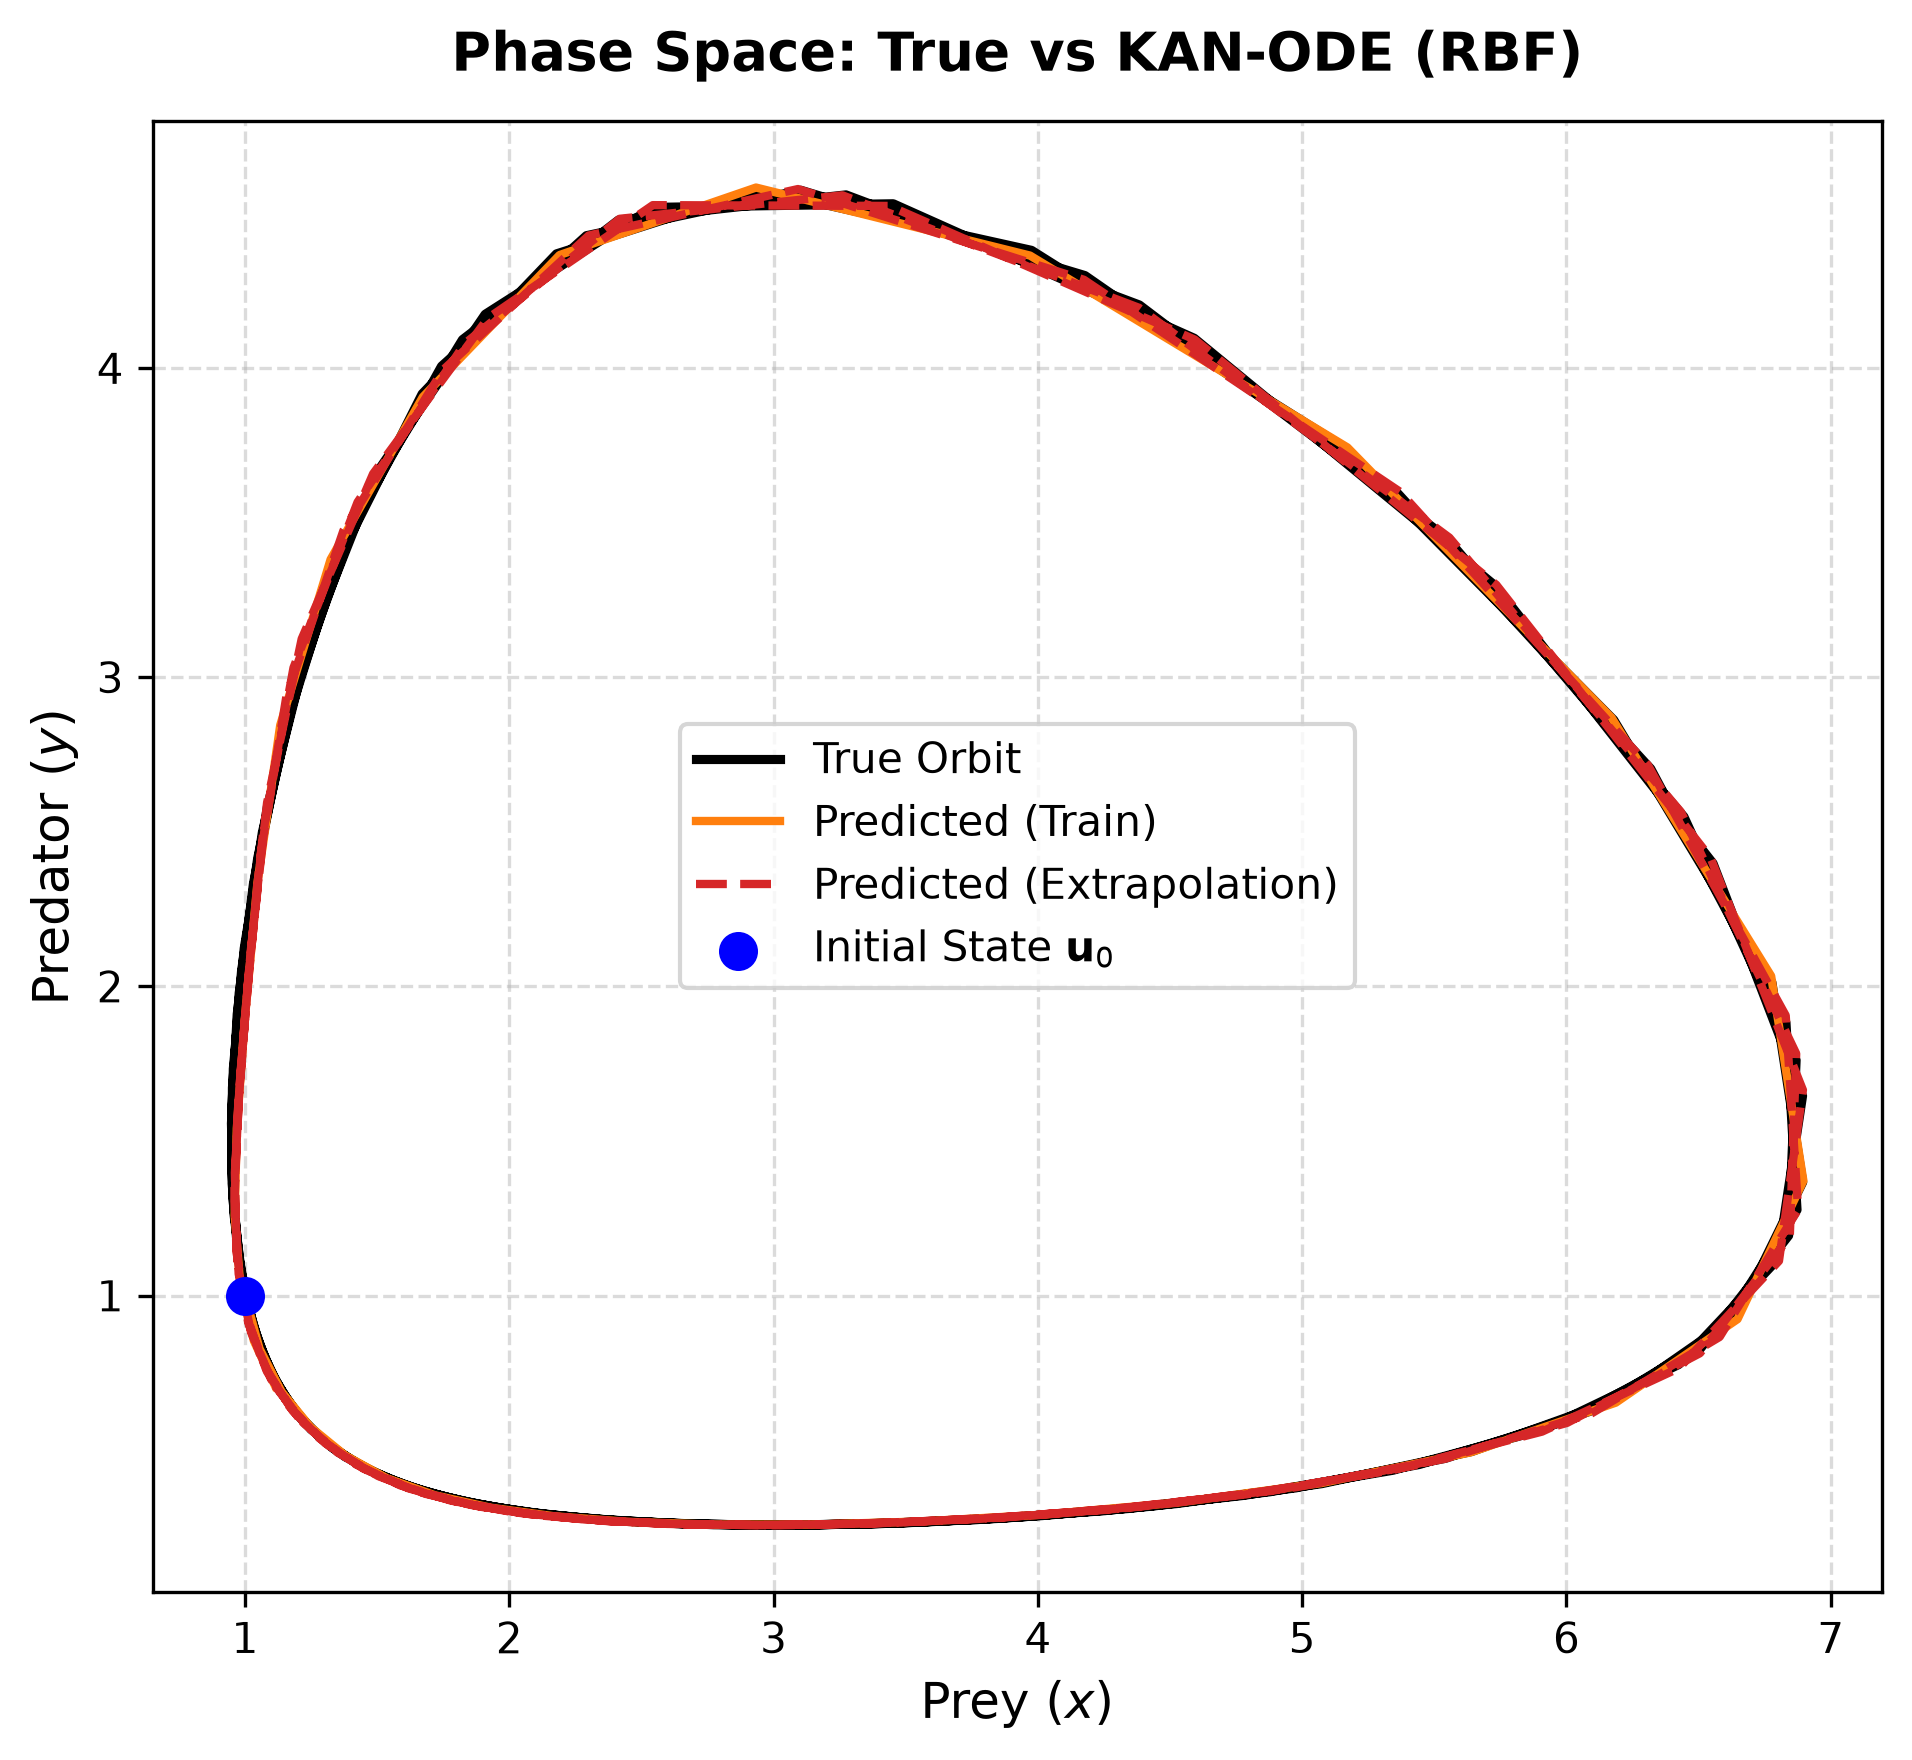
\includegraphics[width=\linewidth]{figures/ablation/solver_tsit5_phase.png}
  \caption{Tsit5 ($p=5$)}
\end{subfigure}
\caption{Phase portraits of the Euler-, Midpoint- and Tsit5-trained RBF
models on $[0,14]$ (all three plots are titled ``KAN-ODE (RBF)'' because the
basis is shared). Each model is integrated with its own training solver.
All three stay on the true orbit to plotting accuracy, including Euler,
whose $28\times$ larger extrapolation MSE is phase error along the orbit
rather than a visible drift off it.}
\label{fig:lv-phase-portraits}
\end{figure*}

\subsection{Basis-function ablation}
\label{sec:basis-results}

We now fix the Tsit5 solver and compare the seven basis families defined in
Section~\ref{sec:bases}, starting with their conditioning and locality.

Figure~\ref{fig:basis-catalog} draws the seven families from the code
itself and reports the 2-norm condition number $\kappa_2(\Psi)$ of the
$400\times G$ design matrix $\Psi_{ng}=B_g(u_n)$ on a uniform sample of
$[-1,1]$. This is the quantity that governs how well-posed fitting the
coefficients $c_g$ is. At $G=5$ Chebyshev ($2.5$), Lagrange ($3.7$) and
B-spline ($5.5$) are well conditioned, the three kernels sit at $8$--$34$,
and Newton is worst at $54$. The growth with $G$ separates them further: at
$G=12$ Chebyshev and B-spline are still below $6$, RBF and Lagrange reach
$69$ and $63$, and Newton reaches $2.4\times10^4$, growing exponentially,
because the nested products $\prod_{j<g}(u-z_j)$ become nearly collinear
columns.

\begin{figure*}[t]
\centering
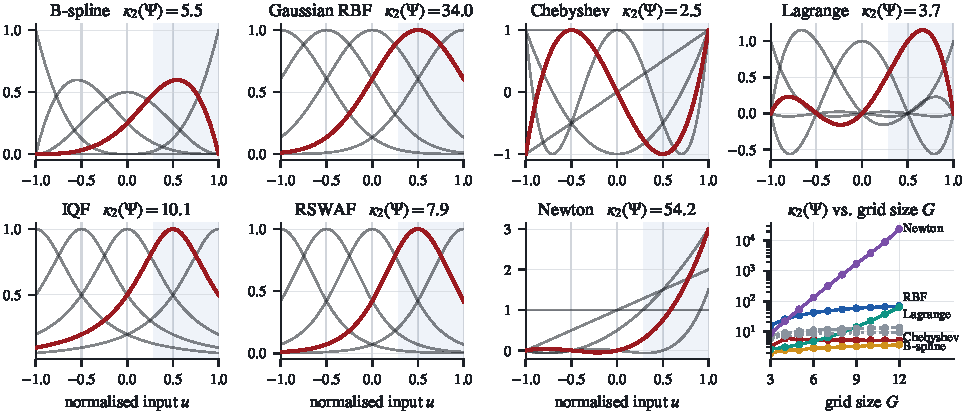
\includegraphics[width=\textwidth]{figures/analysis/basis_catalog.pdf}
\caption{The seven implemented basis families on the $G=5$ grid (vertical
lines are the knots $z_g$), with the $g=4$ function highlighted and the
2-norm condition number of the design matrix in each title. The blue band is
the interval $u\in[0.25,1]$ that first-layer inputs actually reach on the
Lotka-Volterra orbit. The last panel shows $\kappa_2$ against grid size;
dashed and dotted grey lines are IQF and RSWAF.}
\label{fig:basis-catalog}
\end{figure*}

\paragraph{How much of the grid the data uses.} Lotka-Volterra's states are
positive, between $0.26$ and $6.9$ on the orbit, so after the $\tanh$
normaliser the first layer sees only $u\in[0.25,1.0]$, the right
$37.5\%$ of its grid. Measured on the trained RBF model, the two leftmost
basis functions ($z_1=-1$, $z_2=-0.5$) carry $0.4\%$ and $3.6\%$ of the
first layer's total basis activation; for the B-spline the leftmost carries
exactly zero and the next $1.7\%$. The second layer, whose inputs are the
signed hidden activations, uses its grid evenly (every basis function
$18$--$26\%$). Roughly a third of the first layer's 100 spline coefficients
are therefore nearly inert on this system. Figure~\ref{fig:locality} shows
what locality means against that data interval: raising the coefficient of
$z_2$ changes the spline edge by at most $0.021\delta$ on the data, the RBF
edge by $0.32\delta$, and the Chebyshev edge by the full $\delta$.

\begin{figure*}[t]
\centering
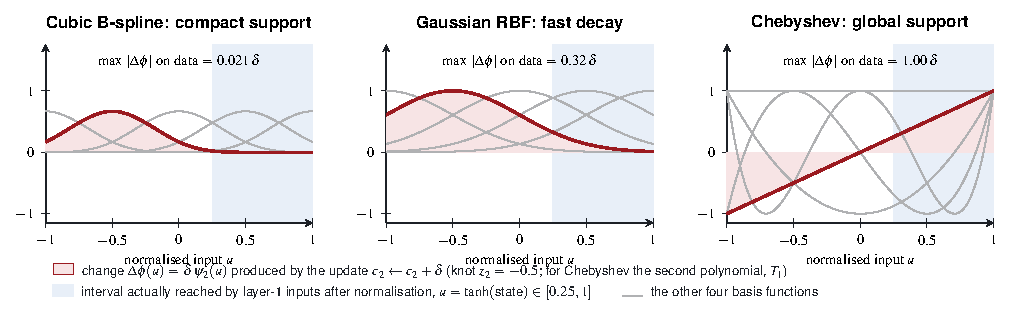
\includegraphics[width=0.85\textwidth]{figures/tikz/local_vs_global_basis.pdf}
\caption{Locality of one coefficient update, $c_2\leftarrow c_2+\delta$,
for three basis families (uniform-knot cubic spline shown for clarity). Since
$\phi$ is linear in $\mathbf{c}$, the change is exactly $\delta\,\psi_2$
(shaded). Compact support confines it to its knot span; the RBF's Gaussian
tail still reaches the data interval (blue); a global polynomial changes the
edge everywhere.}
\label{fig:locality}
\end{figure*}

\begin{table*}[t]
\centering
\footnotesize
\renewcommand{\arraystretch}{1.1}
\caption{Basis ablation (fixed Tsit5 solver, $G=5$ grid points, 240
parameters, $10^4$ epochs). $\kappa_2$ is the design-matrix condition number
of Figure~\ref{fig:basis-catalog}.}
\label{tab:basis-ablation}
\begin{tabularx}{\textwidth}{@{}Y C{2.3cm} C{2.3cm} C{1.7cm} C{1.6cm} C{1.2cm} C{1.2cm} C{1.6cm}@{}}
\toprule
\hdrrow \thh{Basis function} & \thh{Training MSE} & \thh{Extrap.\ MSE} & \thh{$R^2$} & \thh{Rel.\ $L_2$} & \thh{$\hat L$} & \thh{$\kappa_2$} & \thh{Wall-clock}\\
\midrule
Cubic B-spline & $\mathbf{7.20\times10^{-5}}$ & $\mathbf{8.38\times10^{-5}}$ & $\mathbf{0.99997}$ & $\mathbf{0.32\%}$ & $8.44$ & $5.5$ & 6680 s\\
Gaussian RBF & $8.83\times10^{-5}$ & $8.92\times10^{-5}$ & $0.99997$ & $0.33\%$ & $6.91$ & $34.0$ & \textbf{1712 s}\\
Lagrange & $1.07\times10^{-4}$ & $3.93\times10^{-4}$ & $0.99987$ & $0.69\%$ & $6.70$ & $3.7$ & 6829 s\\
Chebyshev & $9.80\times10^{-5}$ & $4.37\times10^{-4}$ & $0.99985$ & $0.73\%$ & $6.48$ & $2.5$ & 2317 s\\
IQF & $2.08\times10^{-4}$ & $9.61\times10^{-4}$ & $0.99967$ & $1.08\%$ & $7.16$ & $10.1$ & 1824 s\\
RSWAF & $1.00\times10^{-4}$ & $1.46\times10^{-3}$ & $0.99950$ & $1.33\%$ & $8.72$ & $7.9$ & 1715 s\\
Newton & $1.47\times10^{-3}$ & $3.65\times10^{-2}$ & $0.98746$ & $6.66\%$ & $5.65$ & $54.2$ & 2187 s\\
\bottomrule
\end{tabularx}
\end{table*}

B-spline edges out RBF on accuracy after a boundary-knot fix, at $3.9\times$
RBF's wall-clock time and a visibly higher Lipschitz estimate ($8.44$ vs.\
$6.91$). Its compact local support lets it fit sharper local features than
RBF's smooth, slowly decaying support without being penalized elsewhere in
the domain. The two bases are statistically tied on error (6\% apart, inside
single-seed noise), which makes RBF the better accuracy-per-second choice.
Polynomial global-support bases (Chebyshev, Lagrange) fit the training
window well and extrapolate $4$--$5\times$ worse. This is the expected
signature of a basis whose every coefficient influences the whole domain
rather than a local region of it. Conditioning alone does not predict the
ranking: Chebyshev is the best-conditioned basis and extrapolates $5\times$
worse than RBF, the worst-conditioned of the working kernels. Locality
matters more than conditioning once $\kappa_2$ is moderate. The two
heavy-tailed kernels, IQF (algebraic $O(r^{-2})$ tails) and RSWAF, train as
well as the polynomials but extrapolate worst among the working bases
($11$--$16\times$ RBF). Newton is the outlier in both directions: it is the
worst-conditioned basis and the only one that never reaches $10^{-3}$
training loss, and its lowest-in-table Lipschitz estimate ($5.65$) reflects
underfitting, not desirable flatness. Figure~\ref{fig:basis-phase} shows the
same ranking in the phase plane.

\begin{figure*}[t]
\centering
\begin{subfigure}[b]{0.24\textwidth}
  \centering
  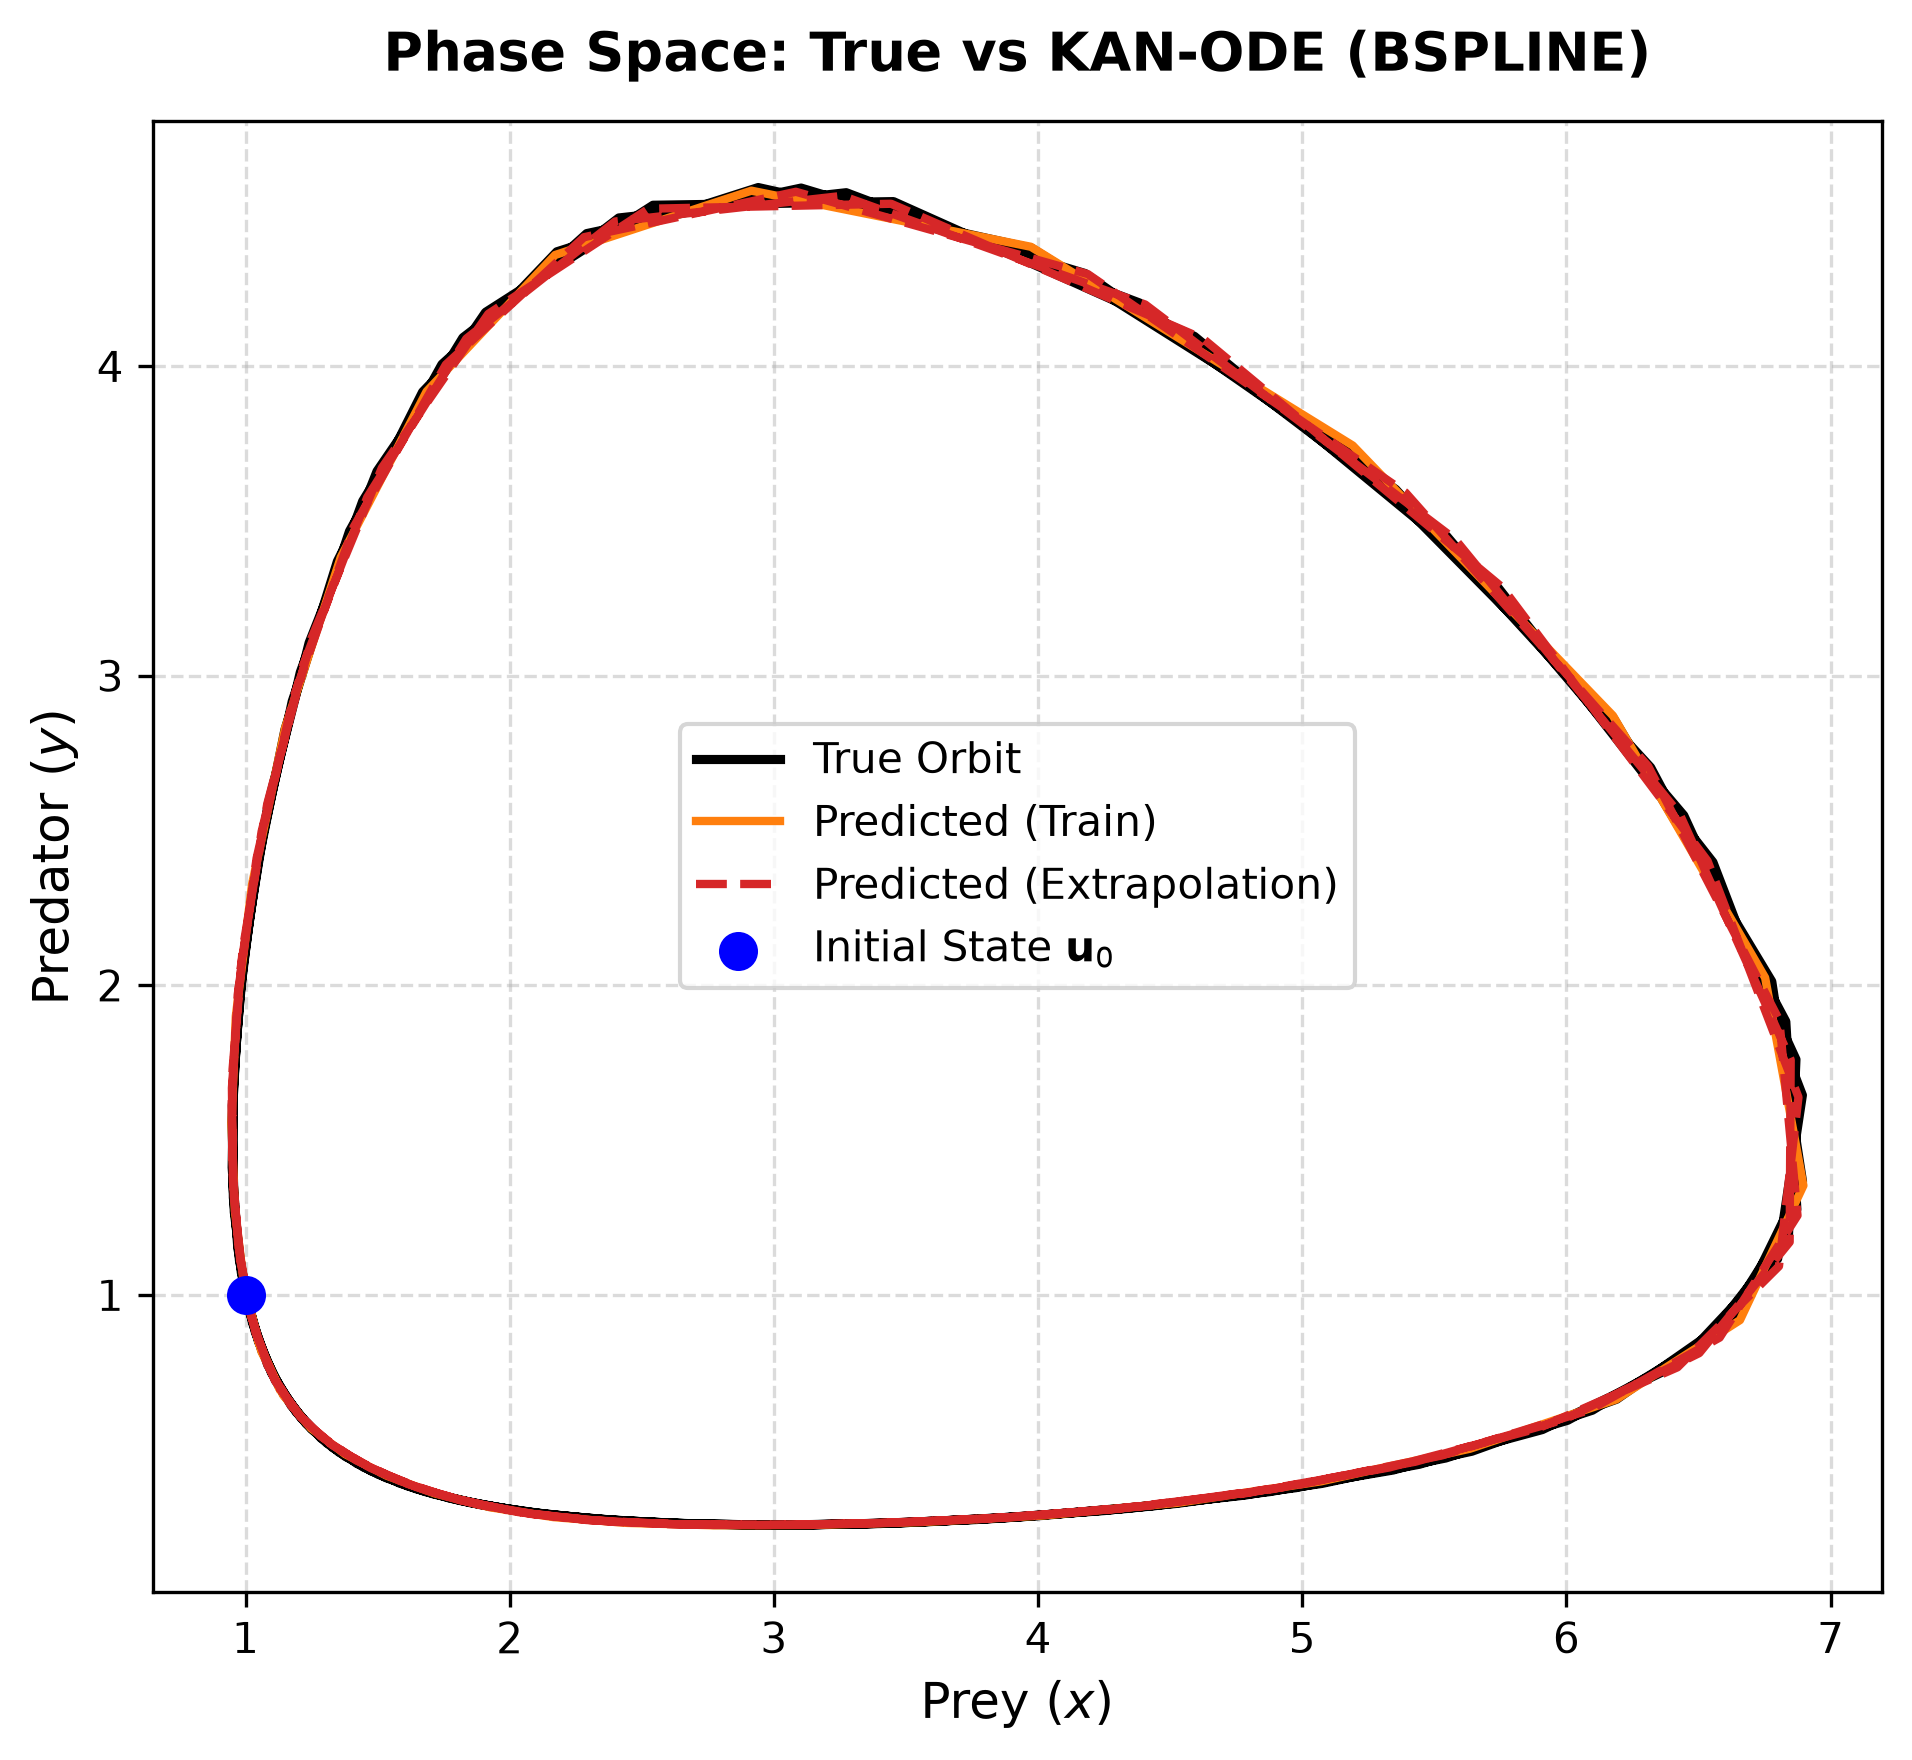
\includegraphics[width=\linewidth]{figures/ablation/basis_bspline_phase.png}
  \caption{Cubic B-spline}
\end{subfigure}\hfill
\begin{subfigure}[b]{0.24\textwidth}
  \centering
  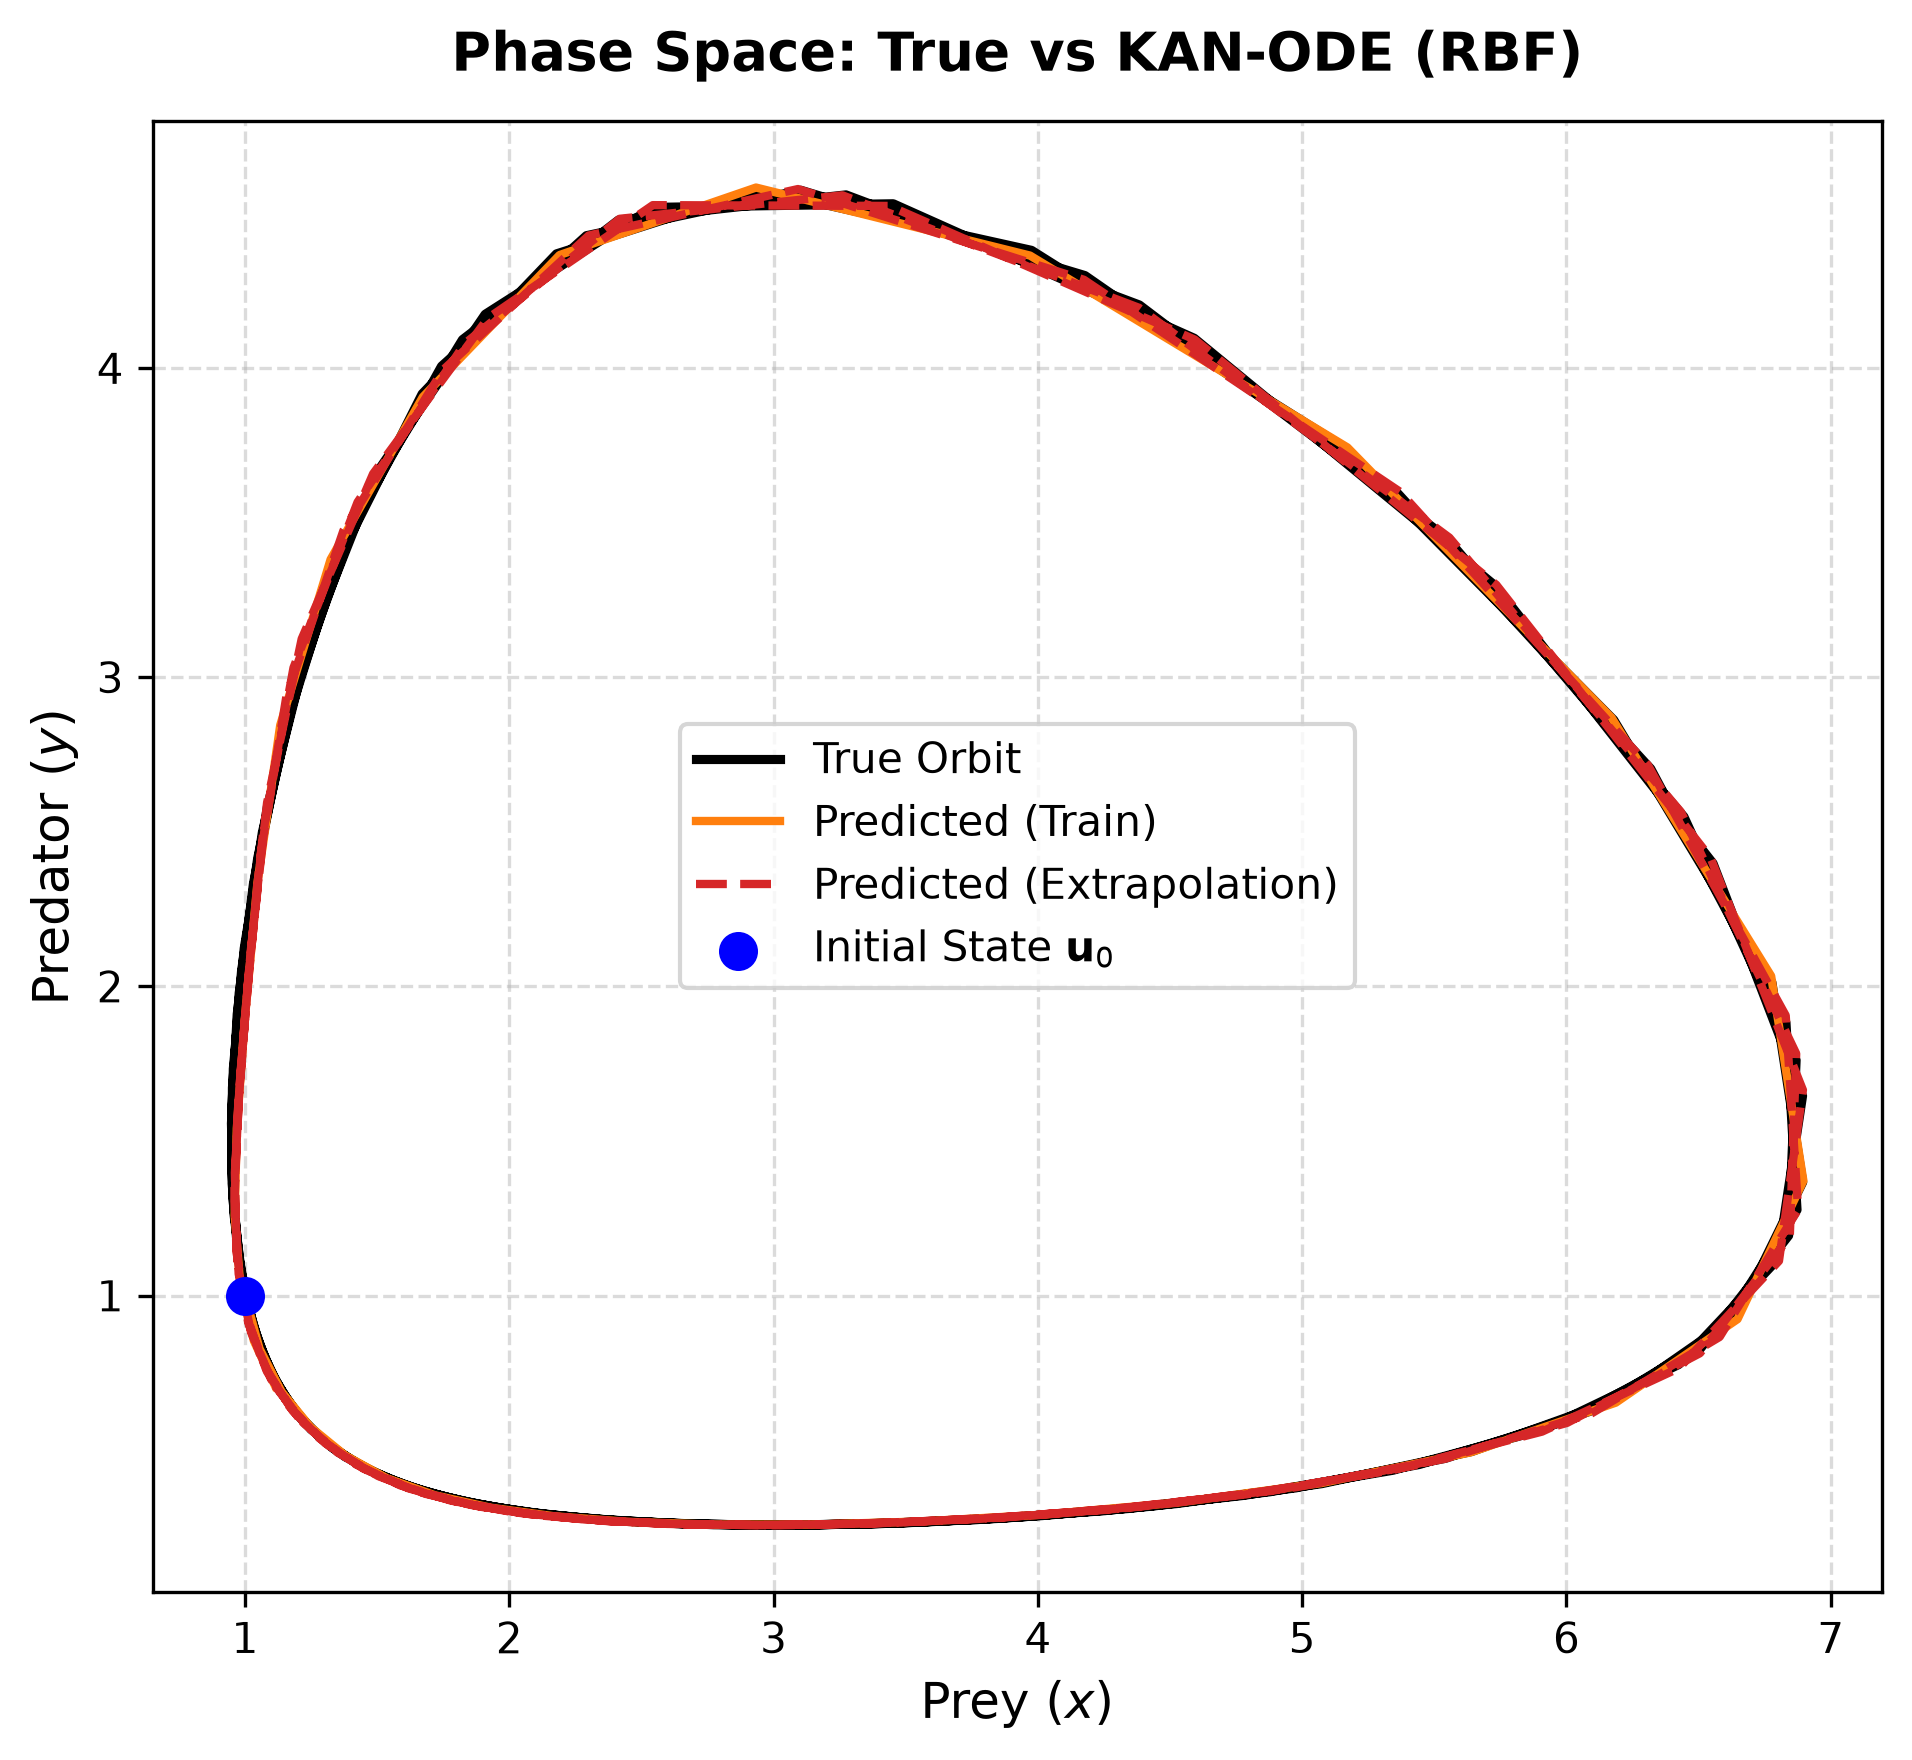
\includegraphics[width=\linewidth]{figures/ablation/basis_rbf_phase.png}
  \caption{Gaussian RBF}
\end{subfigure}\hfill
\begin{subfigure}[b]{0.24\textwidth}
  \centering
  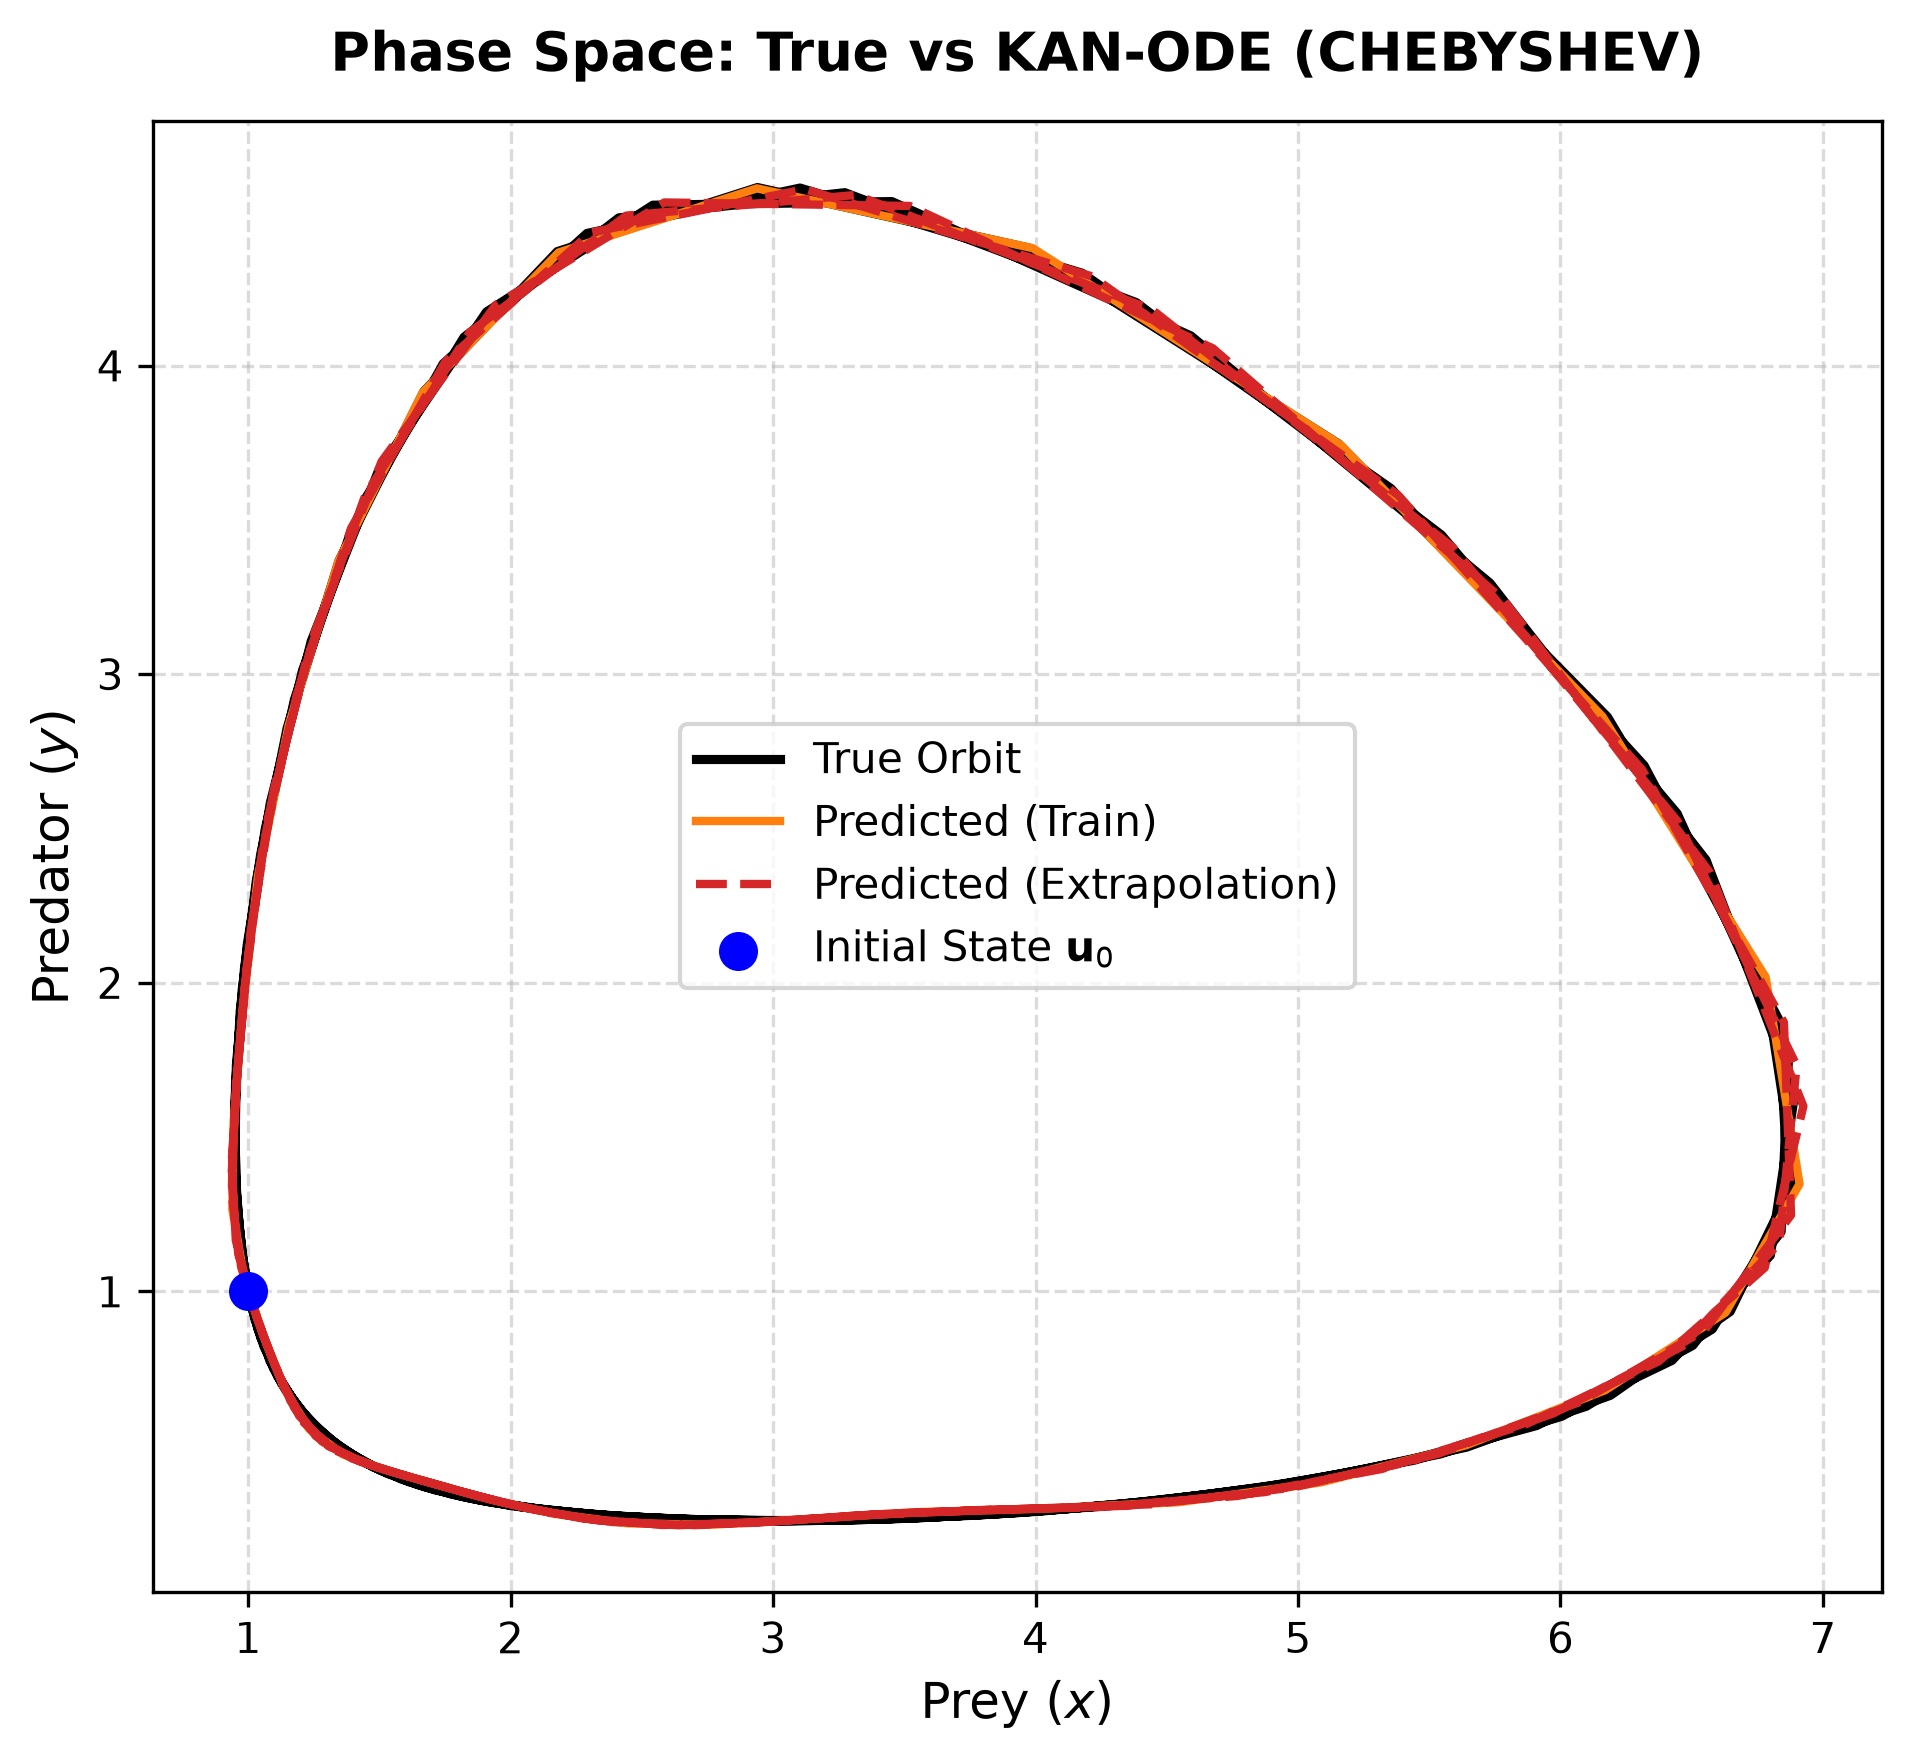
\includegraphics[width=\linewidth]{figures/ablation/basis_chebyshev_phase.png}
  \caption{Chebyshev}
\end{subfigure}\hfill
\begin{subfigure}[b]{0.24\textwidth}
  \centering
  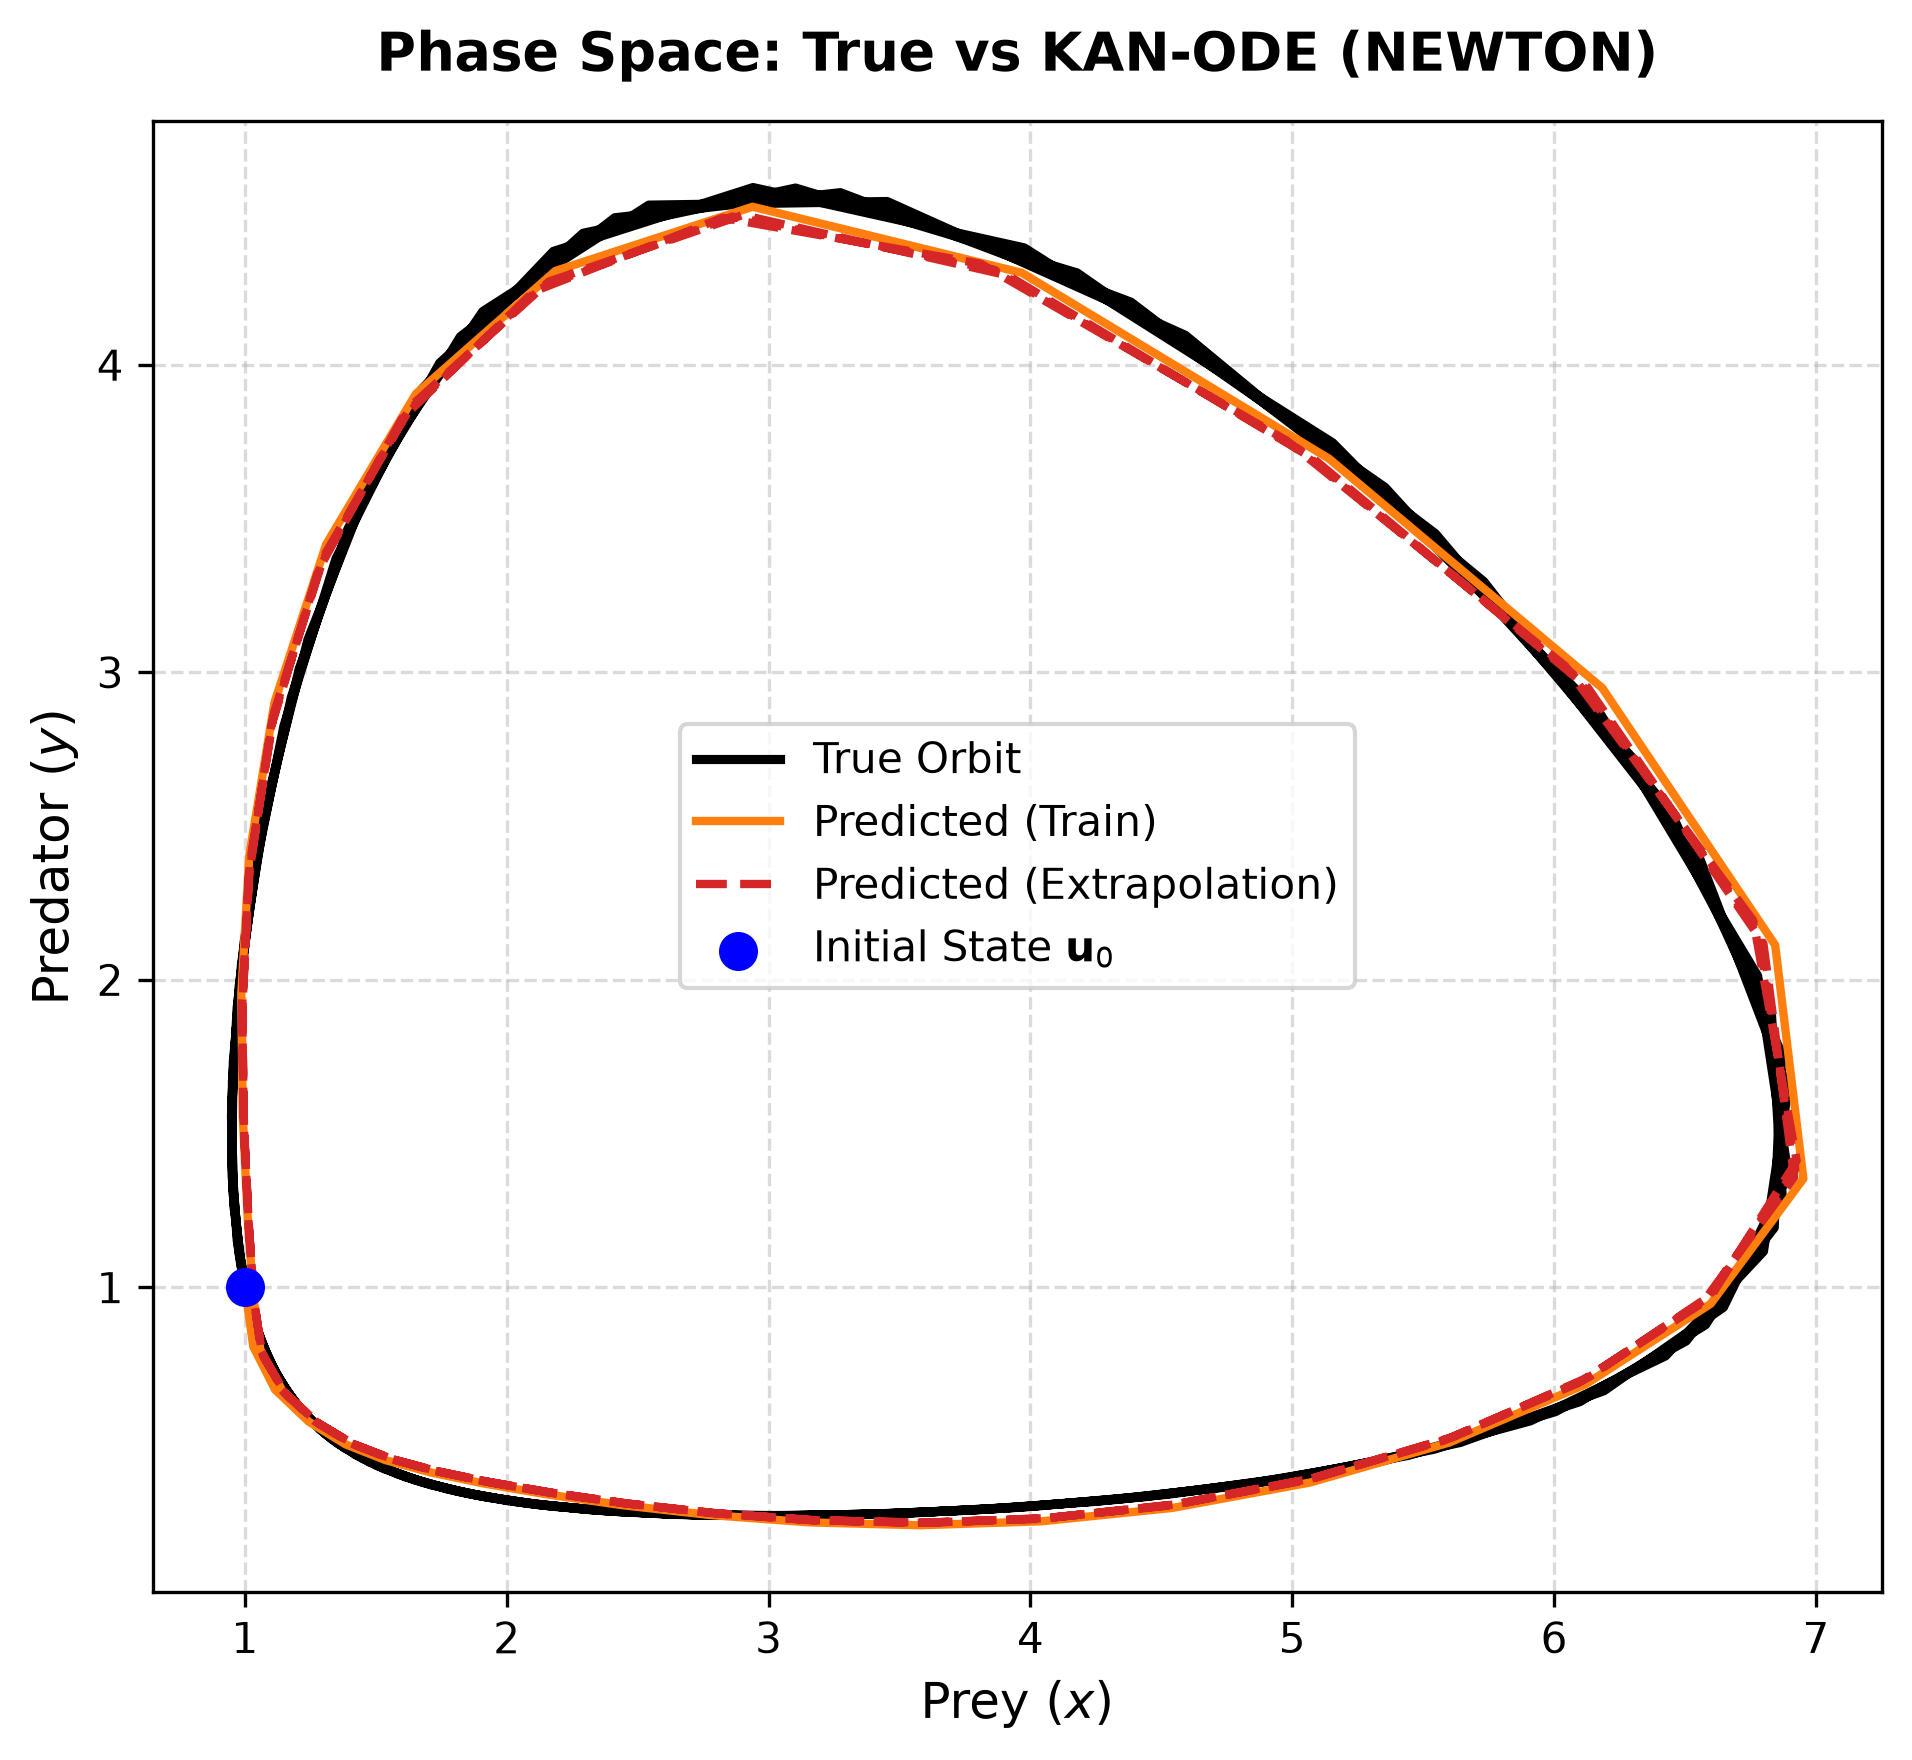
\includegraphics[width=\linewidth]{figures/ablation/basis_newton_phase.png}
  \caption{Newton}
\end{subfigure}
\caption{Phase portraits on $[0,14]$ for four of the seven bases (Tsit5).
B-spline, RBF and Chebyshev all trace the true orbit closely at this scale;
Chebyshev's $5\times$ larger extrapolation error is phase error rather than
a visible departure. The Newton-basis model visibly misses the orbit near
its upper and right-hand extremes.}
\label{fig:basis-phase}
\end{figure*}

\subsection{Step-size and noise sensitivity}
\label{sec:dt-noise}

Two more one-factor sweeps vary the data rather than the model
(Figure~\ref{fig:noise-dt}, Table~\ref{tab:noise-dt}). The \textbf{step-size
sweep} changes the sampling interval $\Delta t$, and with it the number of
training points and the solver step $h=\Delta t/2$. The trend is not
monotone. $\Delta t=0.1$ extrapolates best; $\Delta t=0.05$ is $1.5\times$
worse with twice the data and twice the cost; and $\Delta t=0.2$ reaches the
\emph{lowest} training loss and the worst extrapolation ($5.1\times$). The
work-precision data rule out truncation as the cause: Tsit5's own error on
the true field at these three steps is $2.6\times10^{-18}$, $4.7\times10^{-14}$
and $2.2\times10^{-10}$ in MSE, at least six orders of magnitude below any
learned error. The coarse grid hurts extrapolation because 19 samples
constrain the field less (it fits them more closely and generalises worse).
The fine grid hurts it because the same 10{,}000 epochs buy a similar
training loss on a harder, longer unrolled graph. Here, step size is a
data-density choice, not a numerical-accuracy one.

\begin{table*}[t]
\centering
\footnotesize
\renewcommand{\arraystretch}{1.1}
\caption{Step-size and observation-noise sweeps (Tsit5, RBF, $10^4$ epochs).
Noise is added only to the training window; all errors are measured against
the clean truth.}
\label{tab:noise-dt}
\begin{tabular}{@{}L{3.4cm} C{1.8cm} C{2.3cm} C{2.3cm} C{1.9cm} C{1.4cm} C{2.0cm}@{}}
\toprule
\hdrrow \thh{Configuration} & \thh{Training points} & \thh{Training MSE} & \thh{Extrap.\ MSE} & \thh{Extrap.\ $R^2$} & \thh{$\hat L$} & \thh{Wall-clock}\\
\midrule
$\Delta t=0.05$ ($h=0.025$) & 71 & $9.37\times10^{-5}$ & $1.34\times10^{-4}$ & $0.99995$ & $7.46$ & 3425 s\\
$\Delta t=0.1$ (reference) & 36 & $8.83\times10^{-5}$ & $\mathbf{8.92\times10^{-5}}$ & $0.99997$ & $6.91$ & 1713 s\\
$\Delta t=0.2$ ($h=0.1$) & 19 & $7.83\times10^{-5}$ & $4.51\times10^{-4}$ & $0.99985$ & $6.64$ & 882 s\\
\midrule
$\sigma=0.01$ & 36 & $1.23\times10^{-4}$ & $1.22\times10^{-3}$ & $0.99958$ & $7.18$ & 1686 s\\
$\sigma=0.05$ & 36 & $7.41\times10^{-4}$ & $2.54\times10^{-2}$ & $0.99129$ & $8.69$ & 1672 s\\
$\sigma=0.1$ & 36 & $2.28\times10^{-3}$ & $1.37\times10^{-1}$ & $0.95282$ & $9.55$ & 1534 s\\
\bottomrule
\end{tabular}
\end{table*}

\begin{figure*}[t]
\centering
\begin{minipage}[t]{0.45\textwidth}
\centering
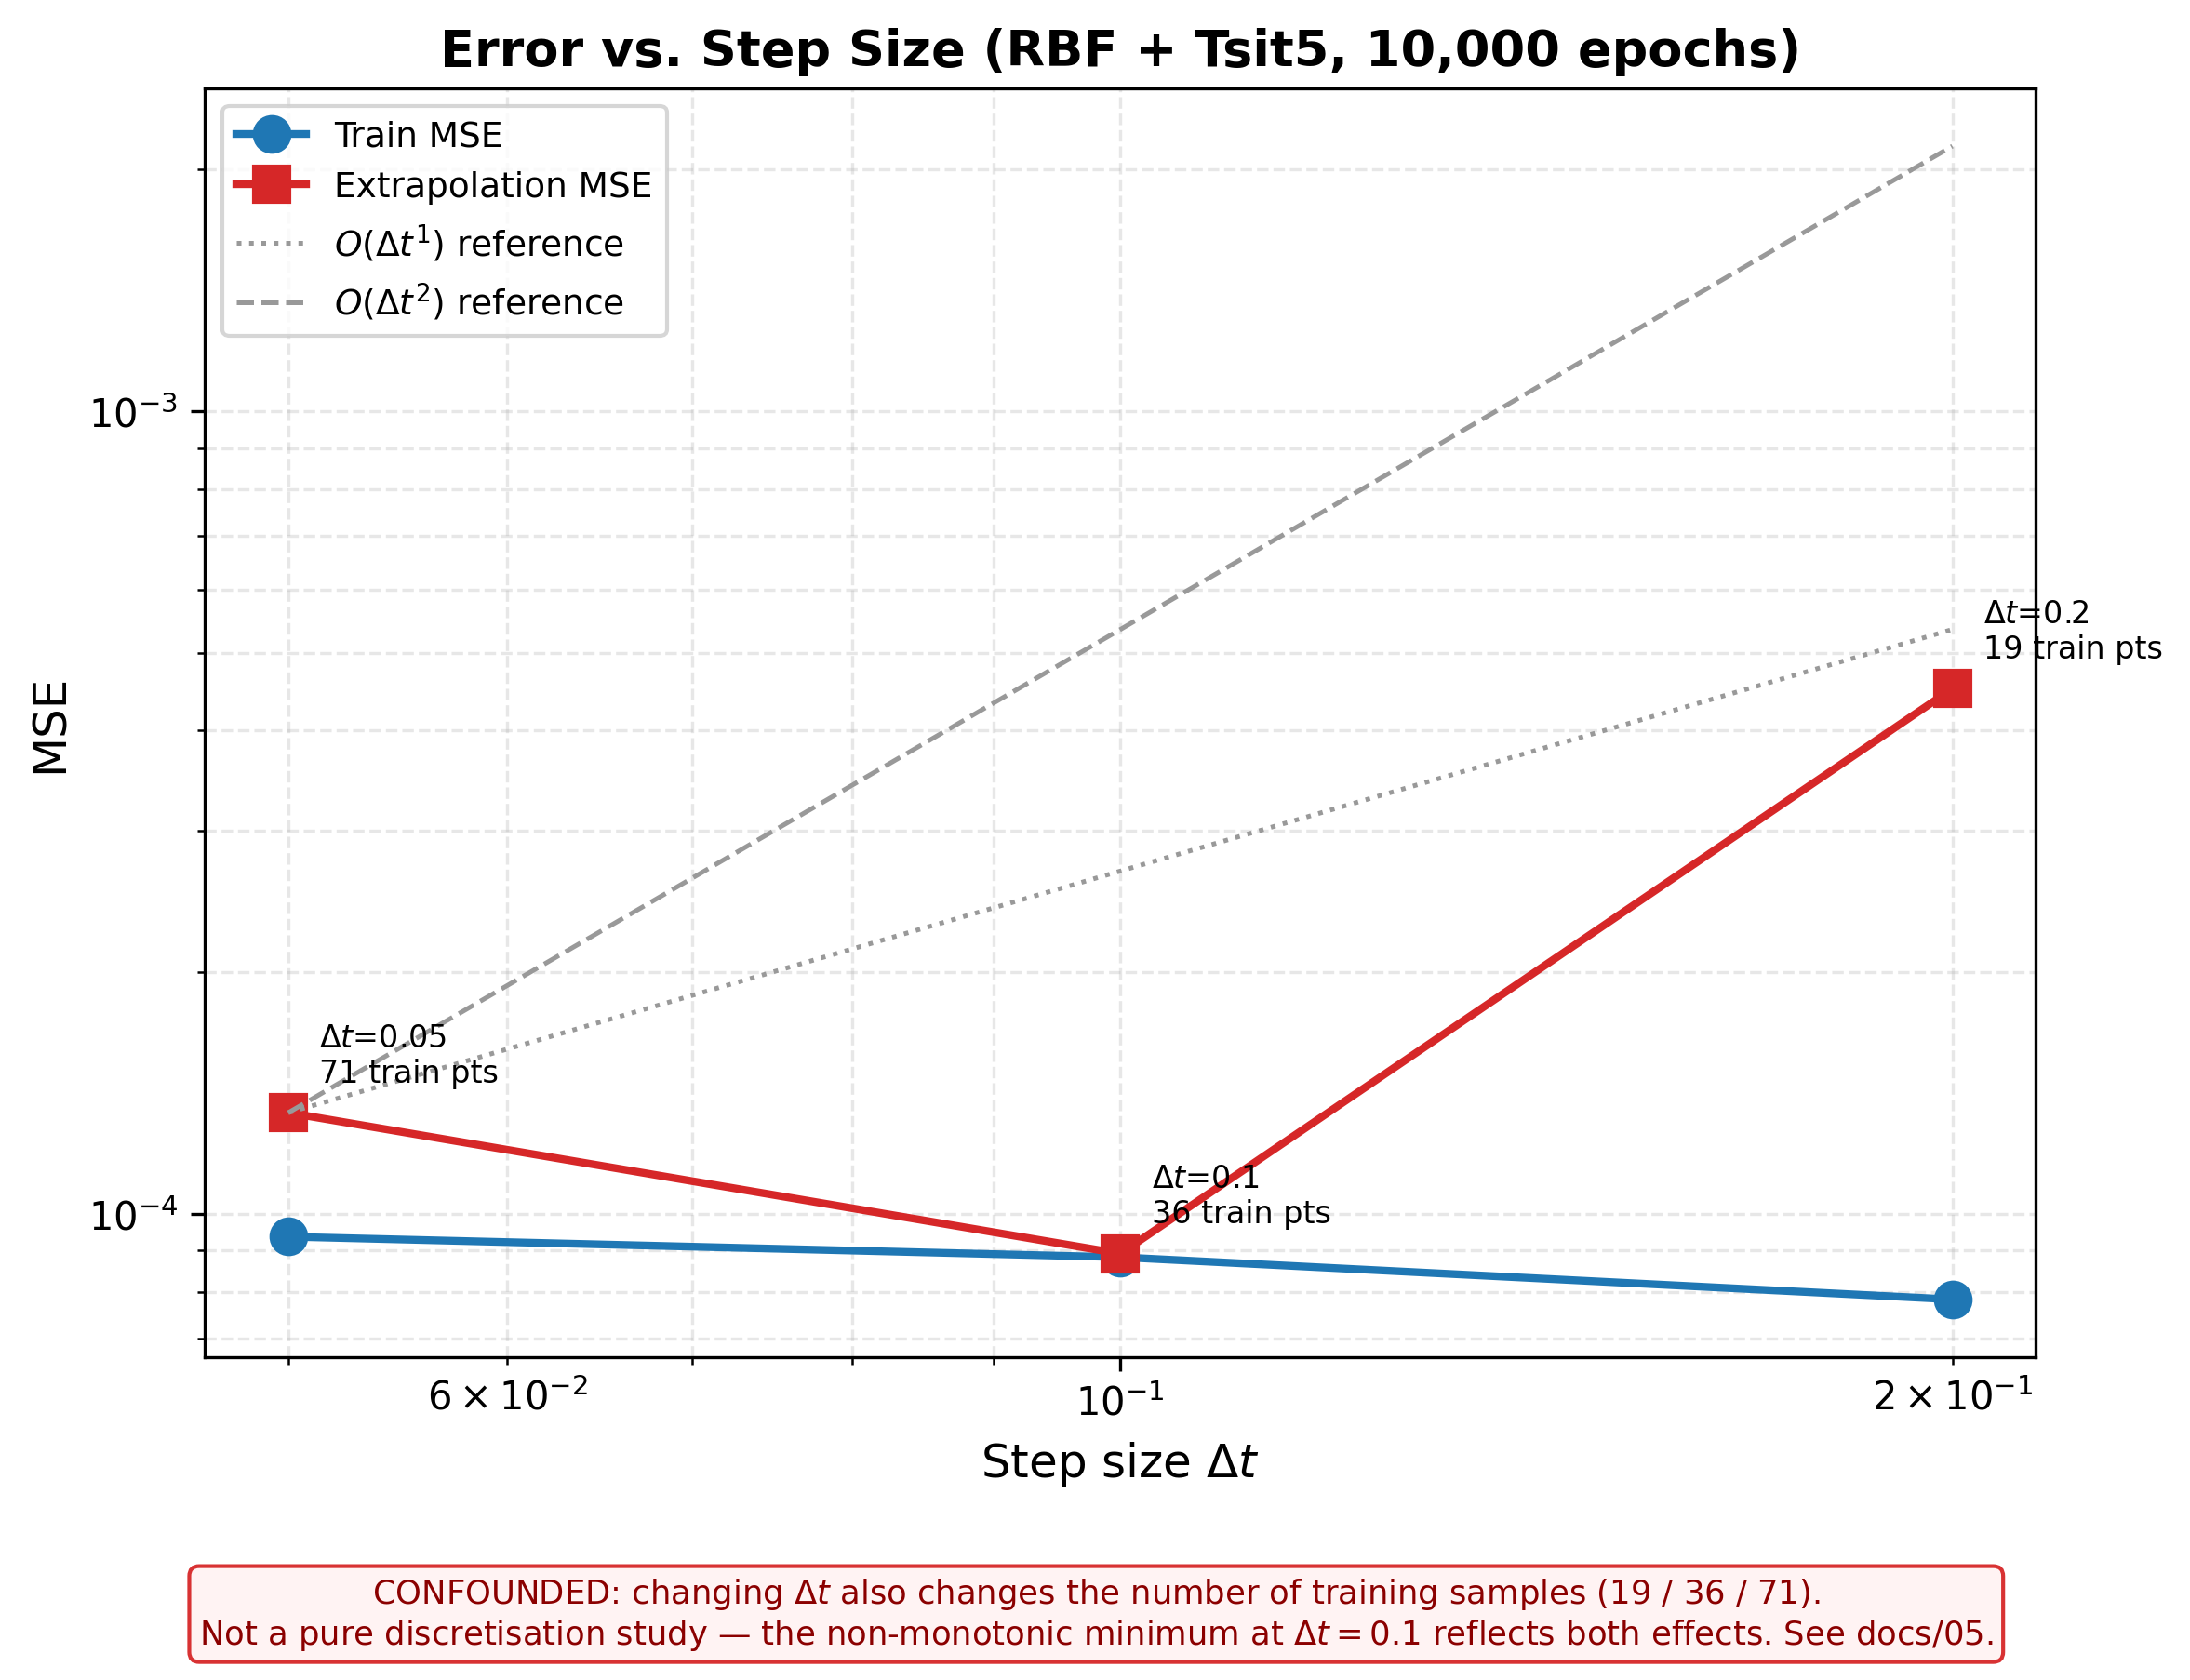
\includegraphics[width=\linewidth]{figures/ablation/02_error_vs_stepsize_loglog.png}
\end{minipage}\hfill
\begin{minipage}[t]{0.45\textwidth}
\centering
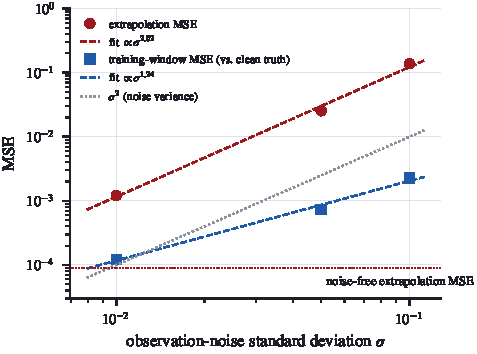
\includegraphics[width=\linewidth]{figures/analysis/noise_sensitivity.pdf}
\end{minipage}
\caption{Left: error against sampling interval, with $O(\Delta t)$ and
$O(\Delta t^2)$ reference slopes; changing $\Delta t$ also changes the
number of training samples. Right: error against observation-noise level,
with least-squares power-law fits; the dotted line is the noise variance
$\sigma^2$.}
\label{fig:noise-dt}
\end{figure*}

The \textbf{noise sweep} adds Gaussian noise of standard deviation $\sigma$
to the 36 training observations. Across $\sigma\in\{0.01,0.05,0.1\}$ the
extrapolation MSE follows a clean power law,
$\mathrm{MSE}_{\text{extrap}}\approx12.9\,\sigma^{2.02}$. In other words,
extrapolation error is proportional to the noise variance, with a gain of
about $13$. The training-window error against the clean truth grows more
slowly ($\propto\sigma^{1.24}$) and sits below $\sigma^2$ at every level
($0.23\sigma^2$ at $\sigma=0.1$), so the ODE constraint does denoise the
fit inside the window. What it cannot do is stop the remaining field error
from compounding into phase error beyond the window. The field also
roughens as it absorbs the noise ($\hat L$ rises from $6.91$ to $9.55$).
Section~\ref{sec:track-e} compares this sensitivity against sparse symbolic
regression.

\subsection{What the trained fields learned}
\label{sec:numerics}

Trajectory error measures one orbit. Because we saved the checkpoints, we
can also examine the learned field $\mathbf{f}_\theta$ itself as a dynamical
system, using the invariants of Section~\ref{sec:datasets} as ground truth.

\paragraph{Equilibria by Newton's method.} We solve
$\mathbf{f}_\theta(\mathbf{u}^\ast)=\mathbf{0}$ by Newton-Raphson,
$\mathbf{u}\leftarrow\mathbf{u}-J_\theta(\mathbf{u})^{-1}\mathbf{f}_\theta(\mathbf{u})$,
with the Jacobian from automatic differentiation in float64, starting at the
true equilibrium $(3,1.5)$. The iteration converges quadratically for every
working model. For the Tsit5 model the residual norms are
$2.1,\ 1.6\times10^{-1},\ 1.1\times10^{-2},\ 9.5\times10^{-6},\ 3.4\times10^{-12}$,
then exactly zero. The residual is roughly squared at every step, which is
the signature of quadratic convergence ($\|\mathbf{F}_{k+1}\|/\|\mathbf{F}_k\|^2$
stays between $0.04$ and $0.43$). The roots, however, are far from the truth
(Table~\ref{tab:equilibria}). Every RBF solver model places its equilibrium
near $(1.9,1.04)$, about $1.15$ from $(3,1.5)$, and it is an unstable focus
with $\mathrm{Re}\,\lambda\approx+1.2$, where the true system has
$\mathrm{Re}\,\lambda=0$. The imaginary parts are close to the true $2.12$.
The Chebyshev and Lagrange models have \emph{stable} foci instead. Newton
iteration on the Chebyshev model does not converge within 30 steps, and on
the Newton-basis model it diverges.

\begin{table*}[t]
\centering
\footnotesize
\renewcommand{\arraystretch}{1.08}
\caption{Numerical analysis of the trained fields. $\mathbf{u}^\ast$:
learned equilibrium (Newton-Raphson from $(3,1.5)$); $\lambda$: eigenvalues
of $J_\theta(\mathbf{u}^\ast)$; period error from zero-crossings of the
predicted prey signal over $[0,28]$; $H$ drift is
$\max_t|H(\hat{\mathbf{u}})-H_0|/H_0$ on $[0,28]$. True values:
$\mathbf{u}^\ast=(3,1.5)$, $\lambda=\pm2.121i$, $T=3.3175$, drift $0$.}
\label{tab:equilibria}
\begin{tabular}{@{}L{4.0cm} C{2.6cm} C{2.0cm} C{1.6cm} C{1.6cm} C{2.0cm} C{1.4cm}@{}}
\toprule
\hdrrow \thh{Model} & \thh{$\mathbf{u}^\ast$} & \thh{$\|\mathbf{u}^\ast-\mathbf{u}^\ast_{\text{true}}\|$} & \thh{$\mathrm{Re}\,\lambda$} & \thh{$|\mathrm{Im}\,\lambda|$} & \thh{Period error} & \thh{$H$ drift}\\
\midrule
Euler & $(1.80,\,1.02)$ & $1.30$ & $+0.51$ & $2.05$ & $-1.7\times10^{-3}$ & $4.2\%$\\
Heun & $(1.91,\,1.03)$ & $1.19$ & $+1.11$ & $2.03$ & $-4.7\times10^{-4}$ & $3.1\%$\\
Midpoint & $(1.93,\,1.04)$ & $1.16$ & $+1.17$ & $2.01$ & $\mathbf{-3.5\times10^{-6}}$ & $3.1\%$\\
RK4 & $(1.94,\,1.05)$ & $1.15$ & $+1.21$ & $1.99$ & $+7.8\times10^{-5}$ & $3.2\%$\\
DOPRI5 & $(1.94,\,1.04)$ & $1.16$ & $+1.20$ & $2.00$ & $+3.5\times10^{-5}$ & $3.2\%$\\
Tsit5 / RBF & $(1.94,\,1.04)$ & $1.15$ & $+1.20$ & $2.01$ & $+1.7\times10^{-5}$ & $3.1\%$\\
\midrule
B-spline & $(1.66,\,0.94)$ & $1.46$ & $+1.18$ & $2.99$ & $+1.3\times10^{-4}$ & $\mathbf{1.3\%}$\\
Lagrange & $(2.67,\,2.15)$ & $0.73$ & $-0.44$ & $5.21$ & $-9.9\times10^{-4}$ & $3.9\%$\\
Chebyshev & \multicolumn{4}{c}{Newton iteration does not converge} & $+6.0\times10^{-4}$ & $5.1\%$\\
IQF & $(2.05,\,1.19)$ & $1.00$ & $+0.26$ & $1.70$ & $-2.2\times10^{-3}$ & $76\%$\\
RSWAF & $(2.15,\,0.91)$ & $1.03$ & $+1.00$ & $1.69$ & $+6.3\times10^{-4}$ & $5.4\%$\\
Newton & \multicolumn{4}{c}{Newton iteration diverges} & $-6.4\times10^{-3}$ & $12\%$\\
\midrule
MLP-ODE (SiLU), $10^4$ & $(2.35,\,1.12)$ & $0.76$ & $+0.30$ & $2.75$ & $+8.0\times10^{-4}$ & $2.8\%$\\
MLP-ODE (tanh, paper), $10^4$ & $(1.64,\,0.79)$ & $1.54$ & $+0.79$ & $2.43$ & $+3.1\times10^{-3}$ & $22.7\%$\\
KAN-ODE, $5\times10^4$ & $(1.51,\,0.80)$ & $1.65$ & $+0.67$ & $2.85$ & $-1.6\times10^{-4}$ & $0.9\%$\\
MLP-ODE (SiLU), $5\times10^4$ & $(3.65,\,1.30)$ & $\mathbf{0.68}$ & $+0.95$ & $1.83$ & $+1.0\times10^{-4}$ & $\mathbf{0.4\%}$\\
MLP-ODE (tanh, paper), $5\times10^4$ & $(1.47,\,0.72)$ & $1.72$ & $+1.09$ & $3.16$ & $+6.8\times10^{-4}$ & $2.8\%$\\
\bottomrule
\end{tabular}
\end{table*}

\paragraph{The learned system is a limit-cycle oscillator.} An unstable
focus surrounded by an orbit that trajectories stay on is the signature of an
attracting limit cycle, not of a conservative centre. We confirm this by
integrating each learned field from four initial conditions whose true orbits
have $H\in\{0.85,\,0.86,\,2.0,\,3.5\}$ (Figure~\ref{fig:limit-cycle}). In the
true system the four orbits are distinct nested curves. Under the KAN and
SiLU fields, at $10^4$ and at $5\times10^4$ epochs, all four
trajectories converge onto the single training orbit, with late-time $H$
between $2.000$ and $2.008$ for every starting point. The paper-settings tanh MLP behaves the same way at $5\times10^4$
epochs (late-time $H=1.998$), but at $10^4$ epochs it captures only
three of the four starting points ($H=2.032$); the trajectory from
$(0.6,0.6)$ diverges. Both architectures
have replaced Lotka-Volterra's one-parameter family of neutral orbits with
one isolated, attracting cycle through the training data. This explains two
things at once. First, the flat extrapolation error of the KAN-ODE
(Table~\ref{tab:extrap-horizon}) is partly a property of the attractor:
amplitude errors are damped back onto the cycle, so only phase error can
accumulate. That is why the period error in Table~\ref{tab:equilibria}
predicts the extrapolation ranking better than any field metric. Second, the
models say nothing reliable about any other initial condition. They have
learned an orbit, not the vector field.

\begin{figure*}[t]
\centering
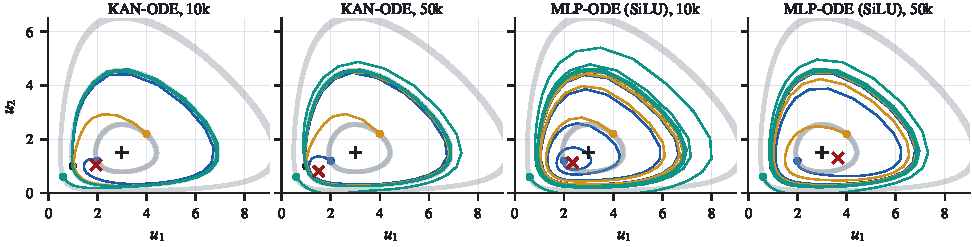
\includegraphics[width=\textwidth]{figures/analysis/limit_cycle_test.pdf}
\caption{Trajectories of each learned field from four initial conditions
(coloured dots) over $t\in[0,40]$, against the four corresponding true orbits
(grey). Red crosses mark the learned equilibria, black plus signs the true
one. Columns: KAN-ODE, SiLU MLP-ODE, and the paper's tanh MLP-ODE under
the paper's own learning rate and initialization; rows: $10^4$ and
$5\times10^4$ epochs. Every learned field attracts all four onto the
training orbit except the $10^4$-epoch tanh MLP, under which the
trajectory from $(0.6,0.6)$ diverges.}
\label{fig:limit-cycle}
\end{figure*}

\paragraph{Where the field is right.} Figure~\ref{fig:field-error} maps the
field error $\|\mathbf{f}_\theta-\mathbf{f}\|$ over the phase plane. It is
small only in a thin tube around the training orbit. On the orbit the error
is $2.7$--$2.8\%$ of the mean field magnitude for the 10k KAN and SiLU
models and $0.6$--$1.1\%$ at 50k; the paper-settings tanh MLP is less
accurate, at $7.0\%$ (10k) and $2.7\%$ (50k). Across the plotted box the
median error is $20$--$34\%$ for KAN and SiLU and $42$--$46\%$ for the
tanh MLP, and for every model less than $3\%$ of the box is below $1\%$
error. Longer training sharpens the tube without widening it: the 50k KAN's
median off-orbit error ($34\%$) is higher than the 10k model's ($24\%$).

\begin{figure*}[t]
\centering
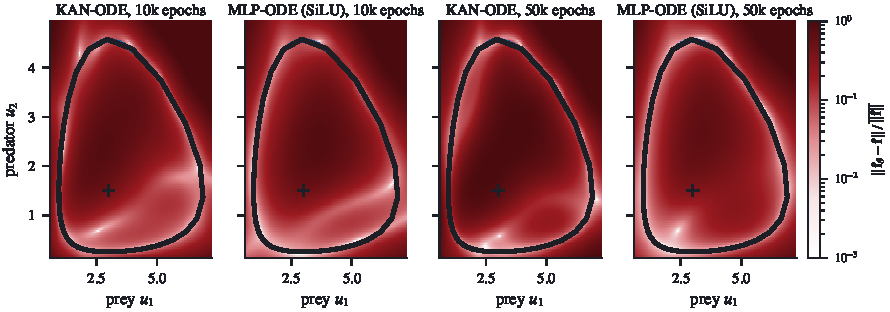
\includegraphics[width=0.9\textwidth]{figures/analysis/field_error_maps.pdf}
\caption{Field error $\|\mathbf{f}_\theta(\mathbf{u})-\mathbf{f}(\mathbf{u})\|$,
normalised by the mean true field magnitude on the orbit ($4.82$), clipped to
$[10^{-3},1]$. Thick black: training segment; blue: rest of the orbit;
plus sign: true equilibrium. Columns and rows as in
Figure~\ref{fig:limit-cycle}.}
\label{fig:field-error}
\end{figure*}

\paragraph{Invariant and error growth.} Figure~\ref{fig:first-integral}b
tracks the first integral along each solver model's own prediction. All of
them hold $H$ to within $3$--$4\%$, and the drift is oscillatory rather than
secular, as it must be on an attracting cycle. The learned models' invariant
error is dominated by model error, orders of magnitude above the solver
drift in panel (a), except for Euler. Figure~\ref{fig:error-vs-time} shows the
pointwise error out to $t=28$. The error envelopes of the Midpoint and Tsit5
models grow by $5.5$--$5.7\times10^{-4}$ per unit time, those of Heun and
Chebyshev by $6$--$8\times10^{-3}$, and Euler's by $2.1\times10^{-2}$.
Panel (b) previews Section~\ref{sec:phase4}. At $5\times10^4$ epochs the MLP
error is lower than the KAN's throughout, while the 50k KAN has a
\emph{larger} far-horizon error than the 10k KAN (maximum $6.5\times10^{-2}$
against $3.4\times10^{-2}$ on $(14,28]$), despite its better scored-window
MSE.

\begin{figure*}[t]
\centering
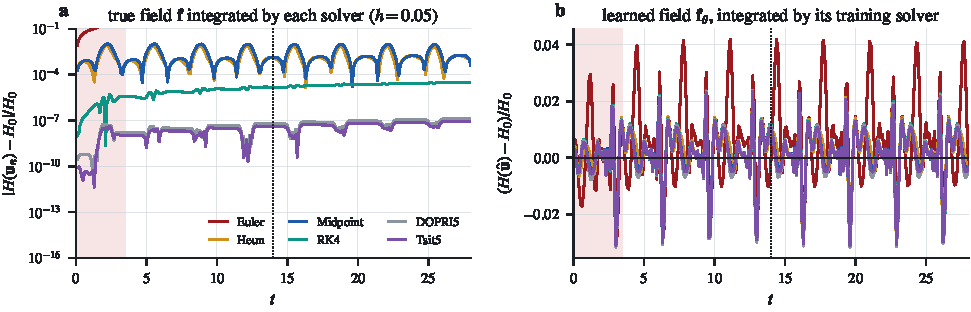
\includegraphics[width=\textwidth]{figures/analysis/first_integral_drift.pdf}
\caption{Relative drift of the Lotka-Volterra first integral $H$
(Equation~\ref{eq:lv-invariant}). (a) The exact field integrated by each
solver at $h=0.05$: pure truncation drift (Euler's trajectory leaves the
domain of $H$ at $t=19.4$). (b) Each trained model integrated by its
training solver. Shaded: training window; dotted: end of the scored horizon.}
\label{fig:first-integral}
\end{figure*}

\begin{figure*}[t]
\centering
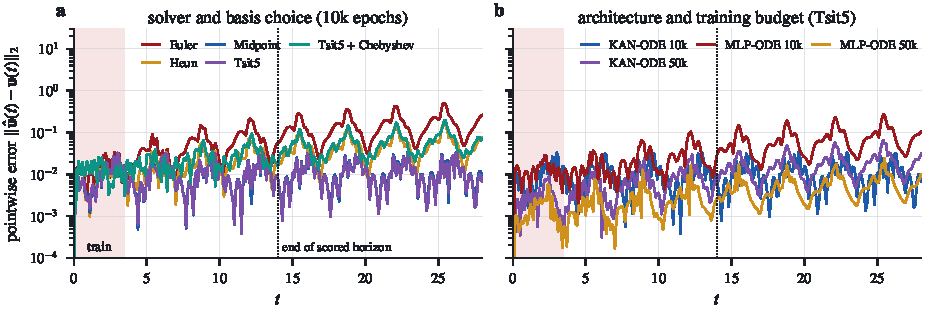
\includegraphics[width=0.9\textwidth]{figures/analysis/error_vs_time.pdf}
\caption{Pointwise trajectory error on $[0,28]$. (a) Solver and basis
choice at $10^4$ epochs (Midpoint and Tsit5 overlap). (b) KAN-ODE and
MLP-ODE at $10^4$ and $5\times10^4$ epochs.}
\label{fig:error-vs-time}
\end{figure*}

\paragraph{What the edges look like.} Figure~\ref{fig:edges} plots the
twenty first-layer edge functions $\phi_{i,j}$ of the RBF and B-spline
models over the range each input covers on the orbit. Over that range most
edges are close to affine, with mild curvature concentrated at small
populations, where $\tanh$ is least saturated. None of them resembles a term
of Equation~\ref{eq:lv}. The bilinear products $u_1u_2$ are assembled by
composition through the second layer rather than carried by any single
edge, which is consistent with the pruning result of
Section~\ref{sec:track-e}.

\begin{figure*}[t]
\centering
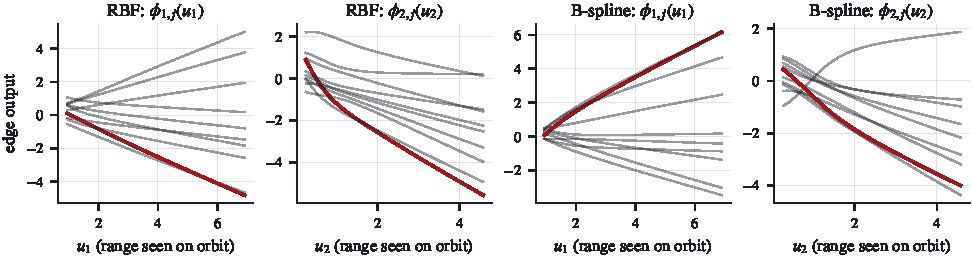
\includegraphics[width=\textwidth]{figures/analysis/edge_functions.pdf}
\caption{First-layer edge functions (spline plus residual branch) of the
trained RBF and B-spline models, each input varied over its range on the
orbit with the other held at its mean. The edge with the largest range is
highlighted.}
\label{fig:edges}
\end{figure*}

\subsubsection{Training dynamics across the sweeps}

Figures~\ref{fig:ablation-curves} and~\ref{fig:basis-curves} show the test
MSE of every configuration during training, and Table~\ref{tab:milestones}
records when each one's training MSE crosses fixed thresholds. Five of the
six solver curves lie on top of each other throughout. Euler separates from
about epoch 2000 and stays above the others until the final approach, so
solver choice changes where training ends rather than how it starts. From
about epoch 6000 every solver shows periodic loss spikes of one to two
orders of magnitude that recover within a few hundred epochs. The basis
curves separate much earlier. B-spline is lowest almost throughout and Newton
highest, and B-spline, Chebyshev and RSWAF reach $10^{-2}$ training MSE
first ($1900$--$2050$ epochs, against RBF's $3112$). Only B-spline turns
that head start into better extrapolation.

\begin{table*}[t]
\centering
\footnotesize
\renewcommand{\arraystretch}{1.08}
\caption{First epoch at which the training MSE falls below each threshold
(``--'': not reached within $10^4$ epochs).}
\label{tab:milestones}
\begin{tabular}{@{}L{2.8cm} C{1.4cm} C{1.4cm} C{1.4cm} @{\hspace{1.2cm}} L{2.8cm} C{1.4cm} C{1.4cm} C{1.4cm}@{}}
\toprule
\hdrrow \thh{Solver} & \thh{$10^{-2}$} & \thh{$10^{-3}$} & \thh{$10^{-4}$} & \thh{Basis} & \thh{$10^{-2}$} & \thh{$10^{-3}$} & \thh{$10^{-4}$}\\
\midrule
Euler & 3533 & 6729 & -- & B-spline & \textbf{1894} & 4826 & \textbf{8458}\\
Heun & 3144 & 5564 & 9512 & Gaussian RBF & 3112 & 5282 & 9617\\
Midpoint & \textbf{3102} & 5285 & 9599 & Chebyshev & 1931 & \textbf{3892} & 9828\\
RK4 & 3153 & 5318 & 9798 & Lagrange & 2924 & 5407 & --\\
DOPRI5 & 3132 & 5305 & 9796 & IQF & 2561 & 5726 & --\\
Tsit5 & 3112 & \textbf{5282} & 9617 & RSWAF & 2047 & 4177 & --\\
MLP-ODE (SiLU) & 741 & 1297 & 9145 & Newton & 4577 & -- & --\\
MLP-ODE (tanh, paper) & 3461 & -- & -- & & & & \\
\bottomrule
\end{tabular}
\end{table*}

\begin{figure}[t]
\centering
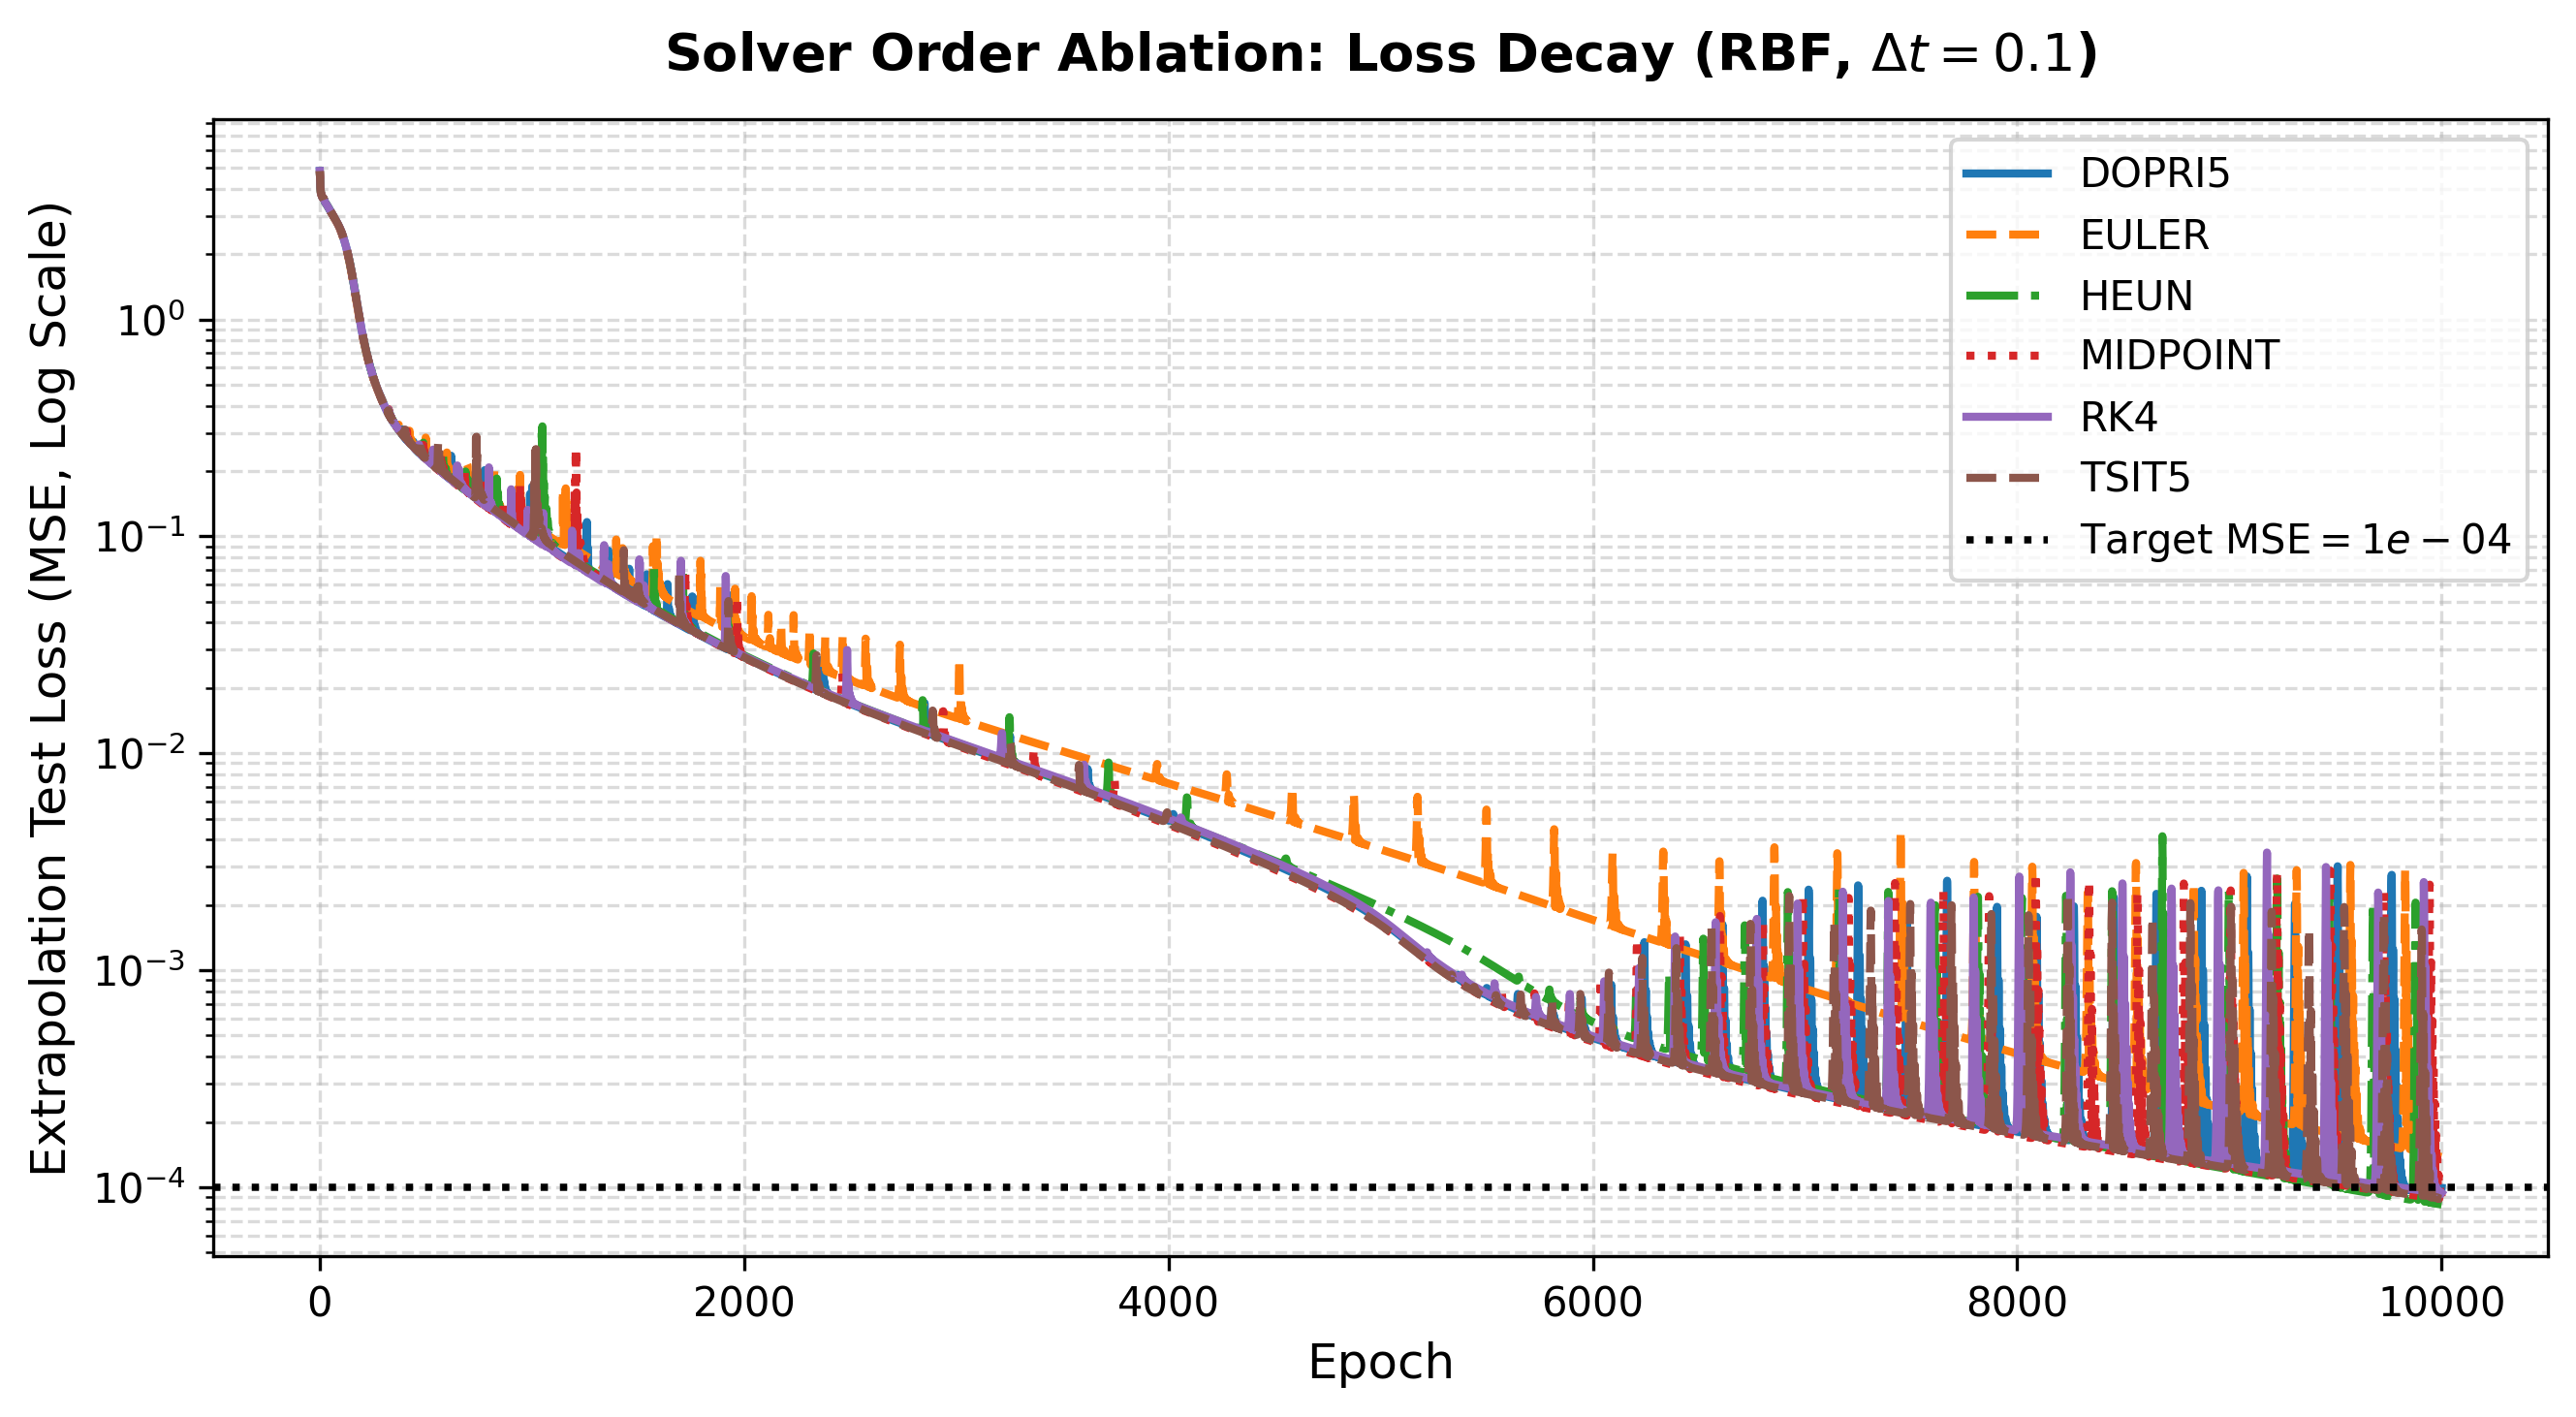
\includegraphics[width=\columnwidth]{figures/ablation/05_solver_convergence.png}
\caption{Test MSE during training for the six solvers (RBF basis),
logged every ten epochs; the dotted line is $10^{-4}$.}
\label{fig:ablation-curves}
\end{figure}

\begin{figure}[t]
\centering
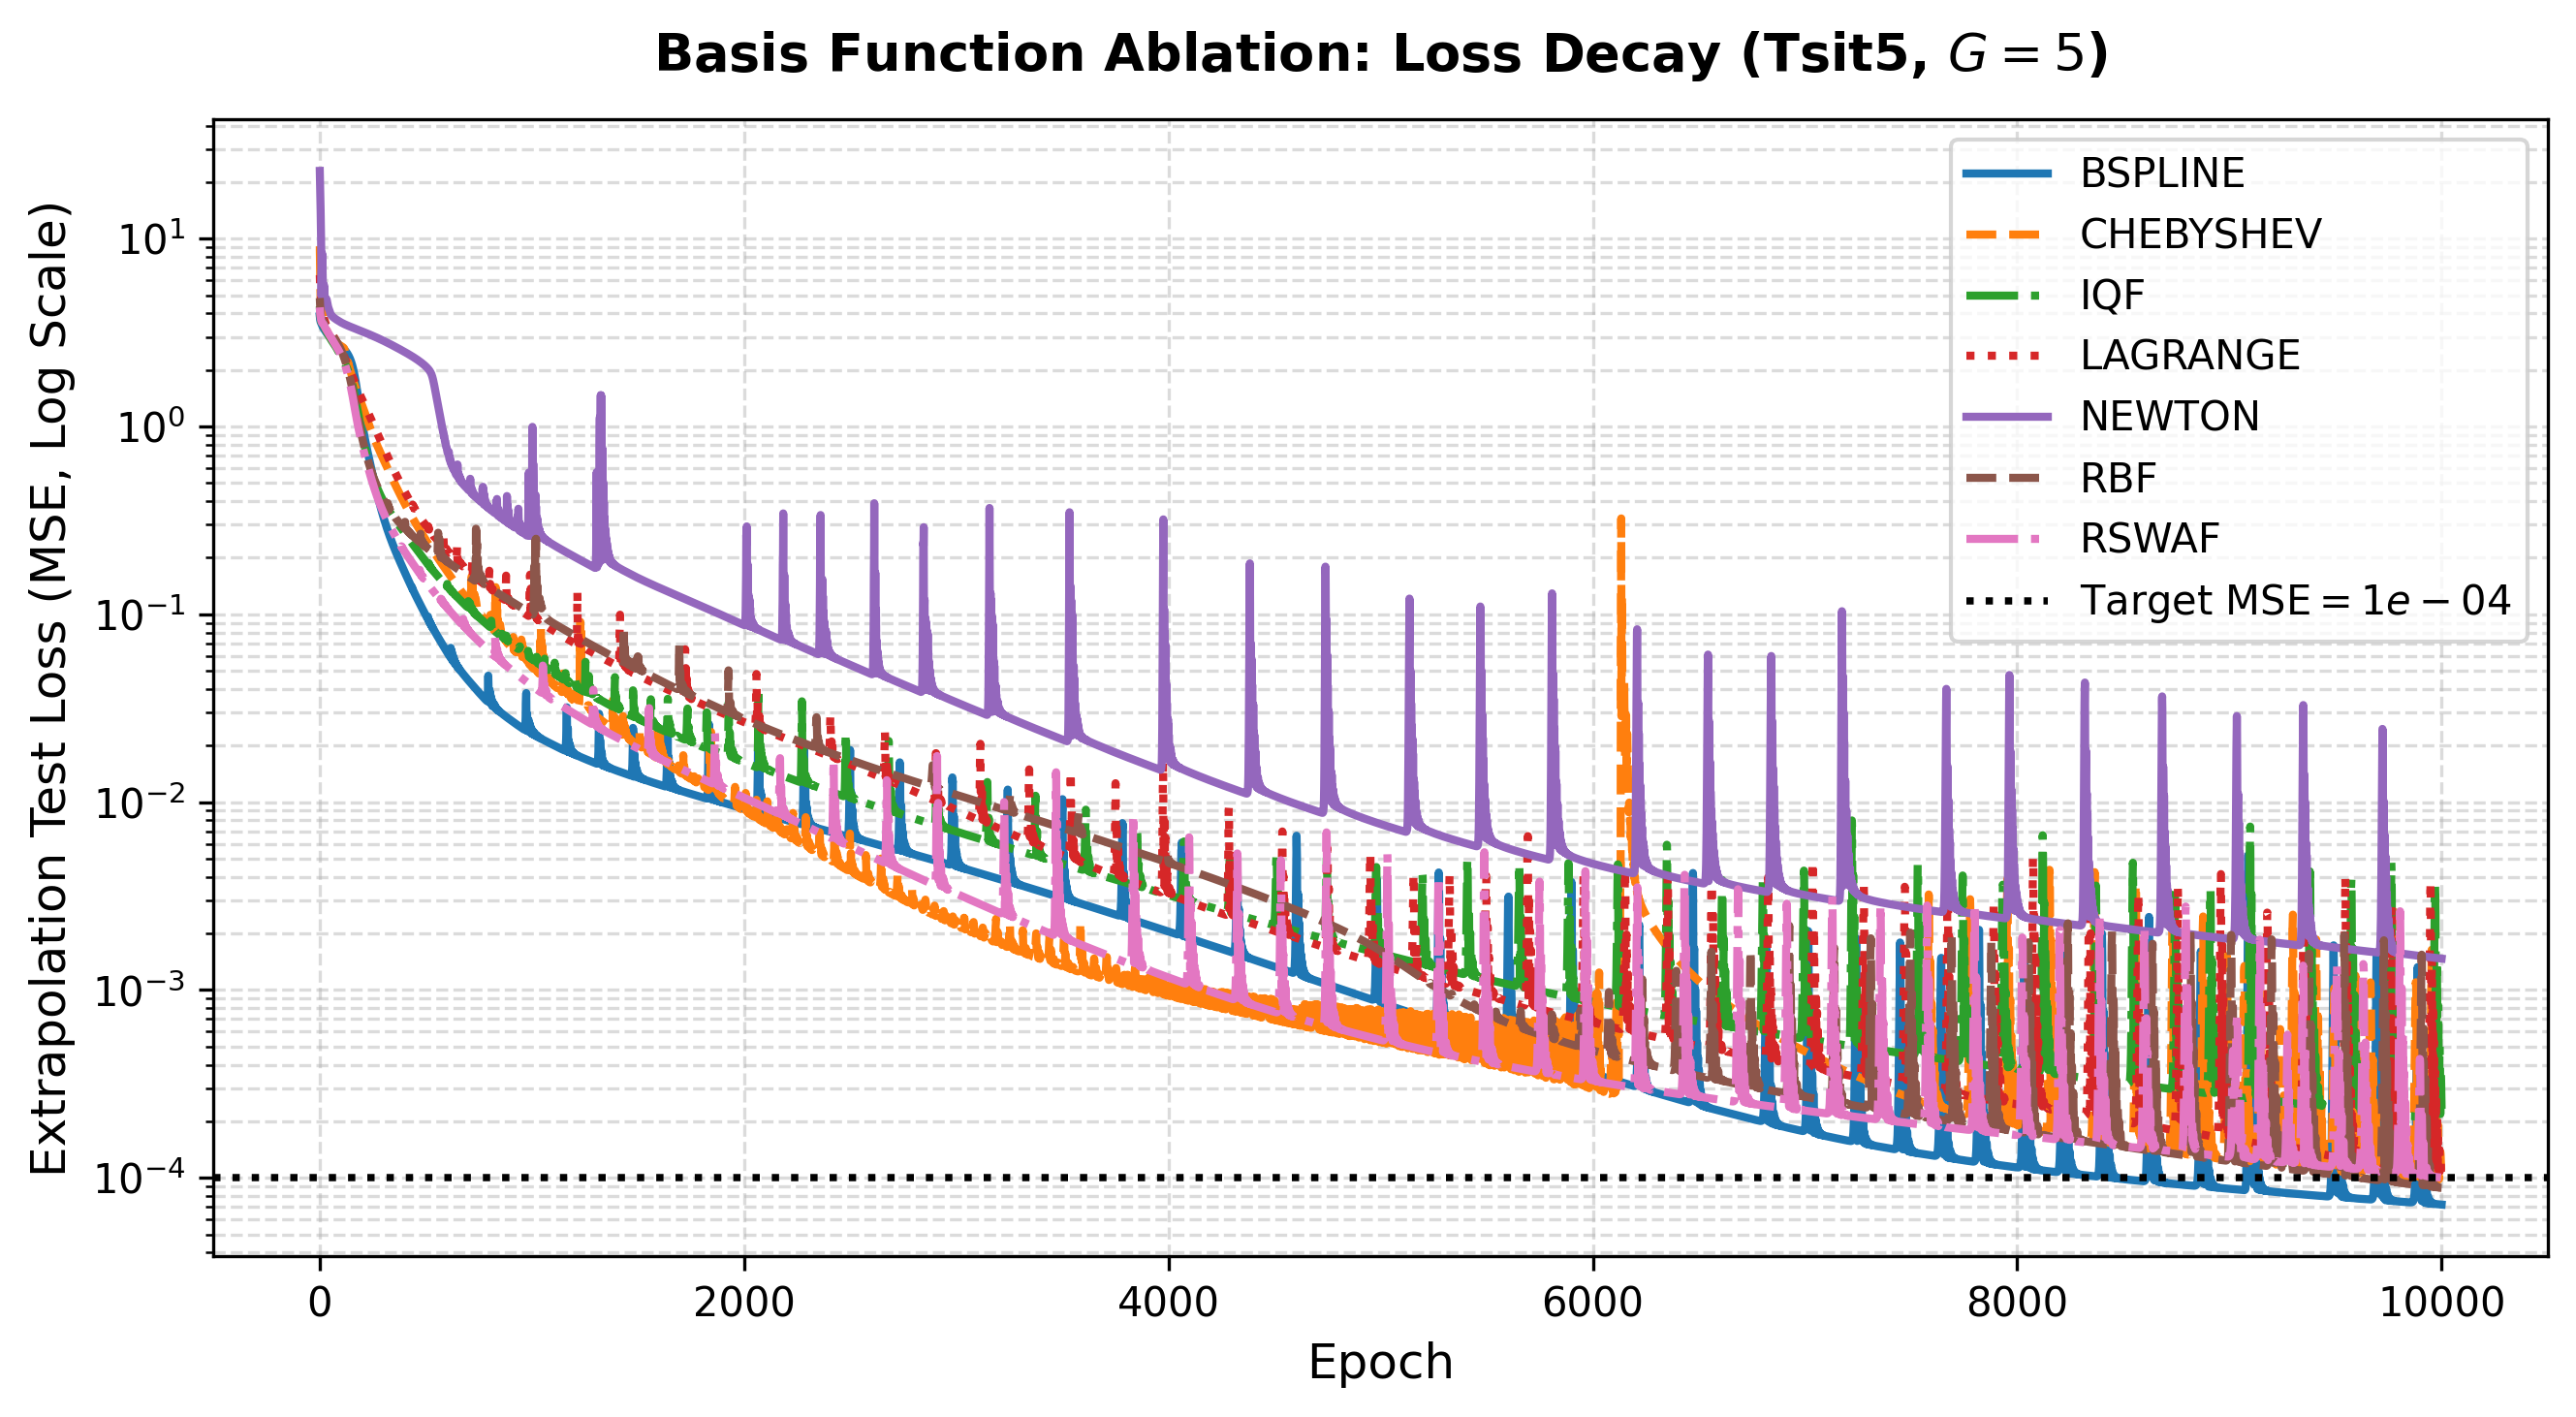
\includegraphics[width=\columnwidth]{figures/ablation/06_basis_convergence.png}
\caption{Test MSE during training for the seven bases (Tsit5 solver),
logged every ten epochs; the dotted line is $10^{-4}$.}
\label{fig:basis-curves}
\end{figure}

\begin{keypoint}[What the ablation and the numerical analysis establish]
\begin{itemize}
\item All six integrators satisfy their order conditions to round-off and
  show their design order; Tsit5's leading error constant is $2.9\times$
  smaller than DOPRI5's.
\item Above order two, solver choice does not change accuracy at $h=0.05$;
  Midpoint is the cost optimum (Tsit5's accuracy at $29\%$ of the time).
\item The network learns the field that its training solver needs, not the
  physical field: the Euler model is an accurate model of the inverse
  modified equation, and models do not transfer across solver families.
\item Locality, not conditioning, separates the bases; on this system a third
  of the first layer's grid is idle because states are positive.
\item Every trained model, KAN or MLP, is an attracting limit-cycle
  oscillator around a spurious unstable equilibrium. It extrapolates the
  training orbit well and says nothing reliable about any other.
\end{itemize}
\end{keypoint}

\subsection{Cross-domain failures and fixes}
\label{sec:crossdomain}

Applying the Lotka-Volterra recipe unchanged to the damped pendulum and to
SIR failed on both systems, each for its own reason. Both diagnoses follow
the same discipline: measure a quantity about the model's behavior
\emph{before} training, rather than search the hyperparameter space after a
failed run.

\paragraph{Pendulum: extending the training window.} The pendulum recipe
originally trained on $t\in[0,3]$ and diverged in extrapolation
($R^2=-1.318$). Extending the training window to $t_{\text{train}}=5.0$, a
single flag, resolves it:

\begin{expectbox}
\expectrow{Question}{Why does the Lotka-Volterra recipe, applied unchanged, diverge on the pendulum?}
\expectrow{Expected (hypothesis)}{SiLU's residual branch cannot represent the sign-changing derivative $\dot\theta=\omega$ -- an architectural limit.}
\expectrow{Observed}{Refuted. A longer training window fixes it under either activation; SiLU fits the sign change fine once the window is long enough.}
\end{expectbox}

\begin{table}[t]
\centering
\footnotesize
\renewcommand{\arraystretch}{1.2}
\caption{Pendulum fix: best configuration versus the original failure.}
\label{tab:pendulum-fix}
\begin{tabularx}{\columnwidth}{@{}Y C{1.9cm} C{1.5cm} C{1.3cm}@{}}
\toprule
\hdrrow \thh{Configuration} & \thh{Full-horizon MSE} & \thh{Extrapolation $R^2$} & \thh{Verdict}\\
\midrule
Original ($t_{\text{train}}=3.0$) & $8.99\times10^{-1}$ & $-1.318$ & diverges\\
Extended window ($t_{\text{train}}=5.0$, SiLU) & $\mathbf{4.48\times10^{-2}}$ & $\mathbf{+0.647}$ & \textbf{adopted}\\
\bottomrule
\end{tabularx}
\end{table}

An earlier hypothesis held that SiLU's residual branch $W\cdot\mathrm{silu}(x)$
cannot represent a sign-changing derivative such as $\dot\theta=\omega$. A
factorial control that crosses activation with training-window length
refutes it directly. With the longer window, SiLU reaches an angular-velocity
root-mean-square error of $0.0114$ radians and reproduces the true turning
point ($\theta_{\min}=-1.380$ against a true value of $-1.385$). The training
window is what fixes the pendulum. The activation choice affects only how
quickly the fit is reached: the identity activation converges
$\sim\!1000\times$ faster at the short window, but does not match the longer
window's accuracy.

\begin{figure*}[t]
\centering
\begin{minipage}[t]{0.48\textwidth}
\centering
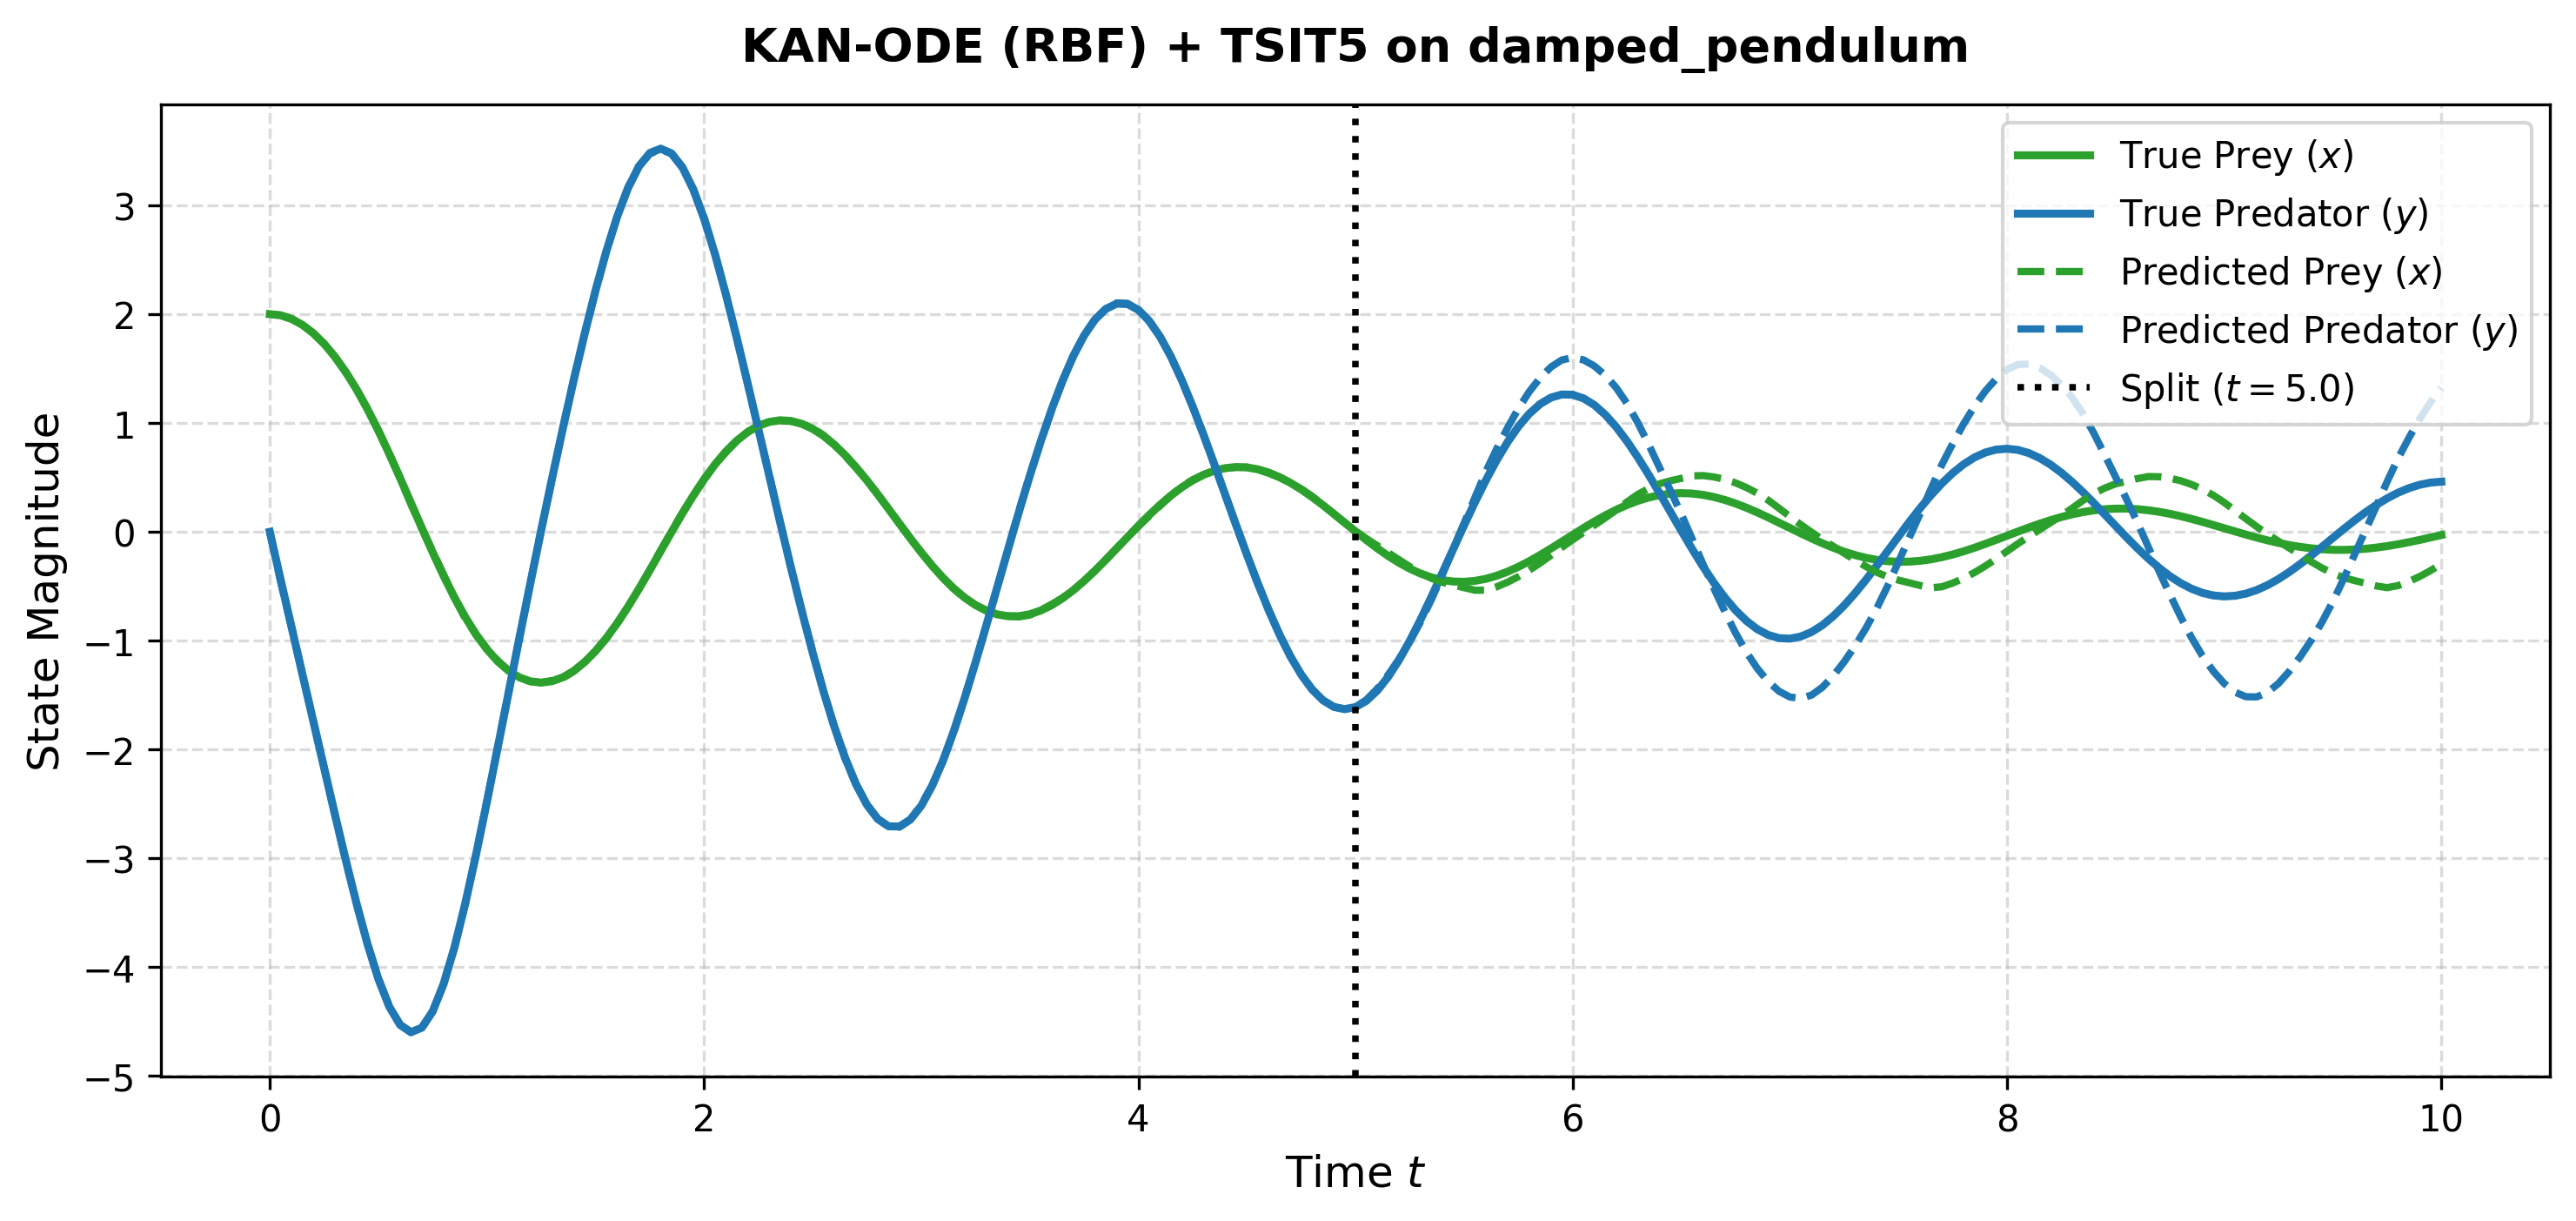
\includegraphics[width=\linewidth]{figures/phase2/pendulum_fixed_trajectory.png}
\end{minipage}\hfill
\begin{minipage}[t]{0.48\textwidth}
\centering
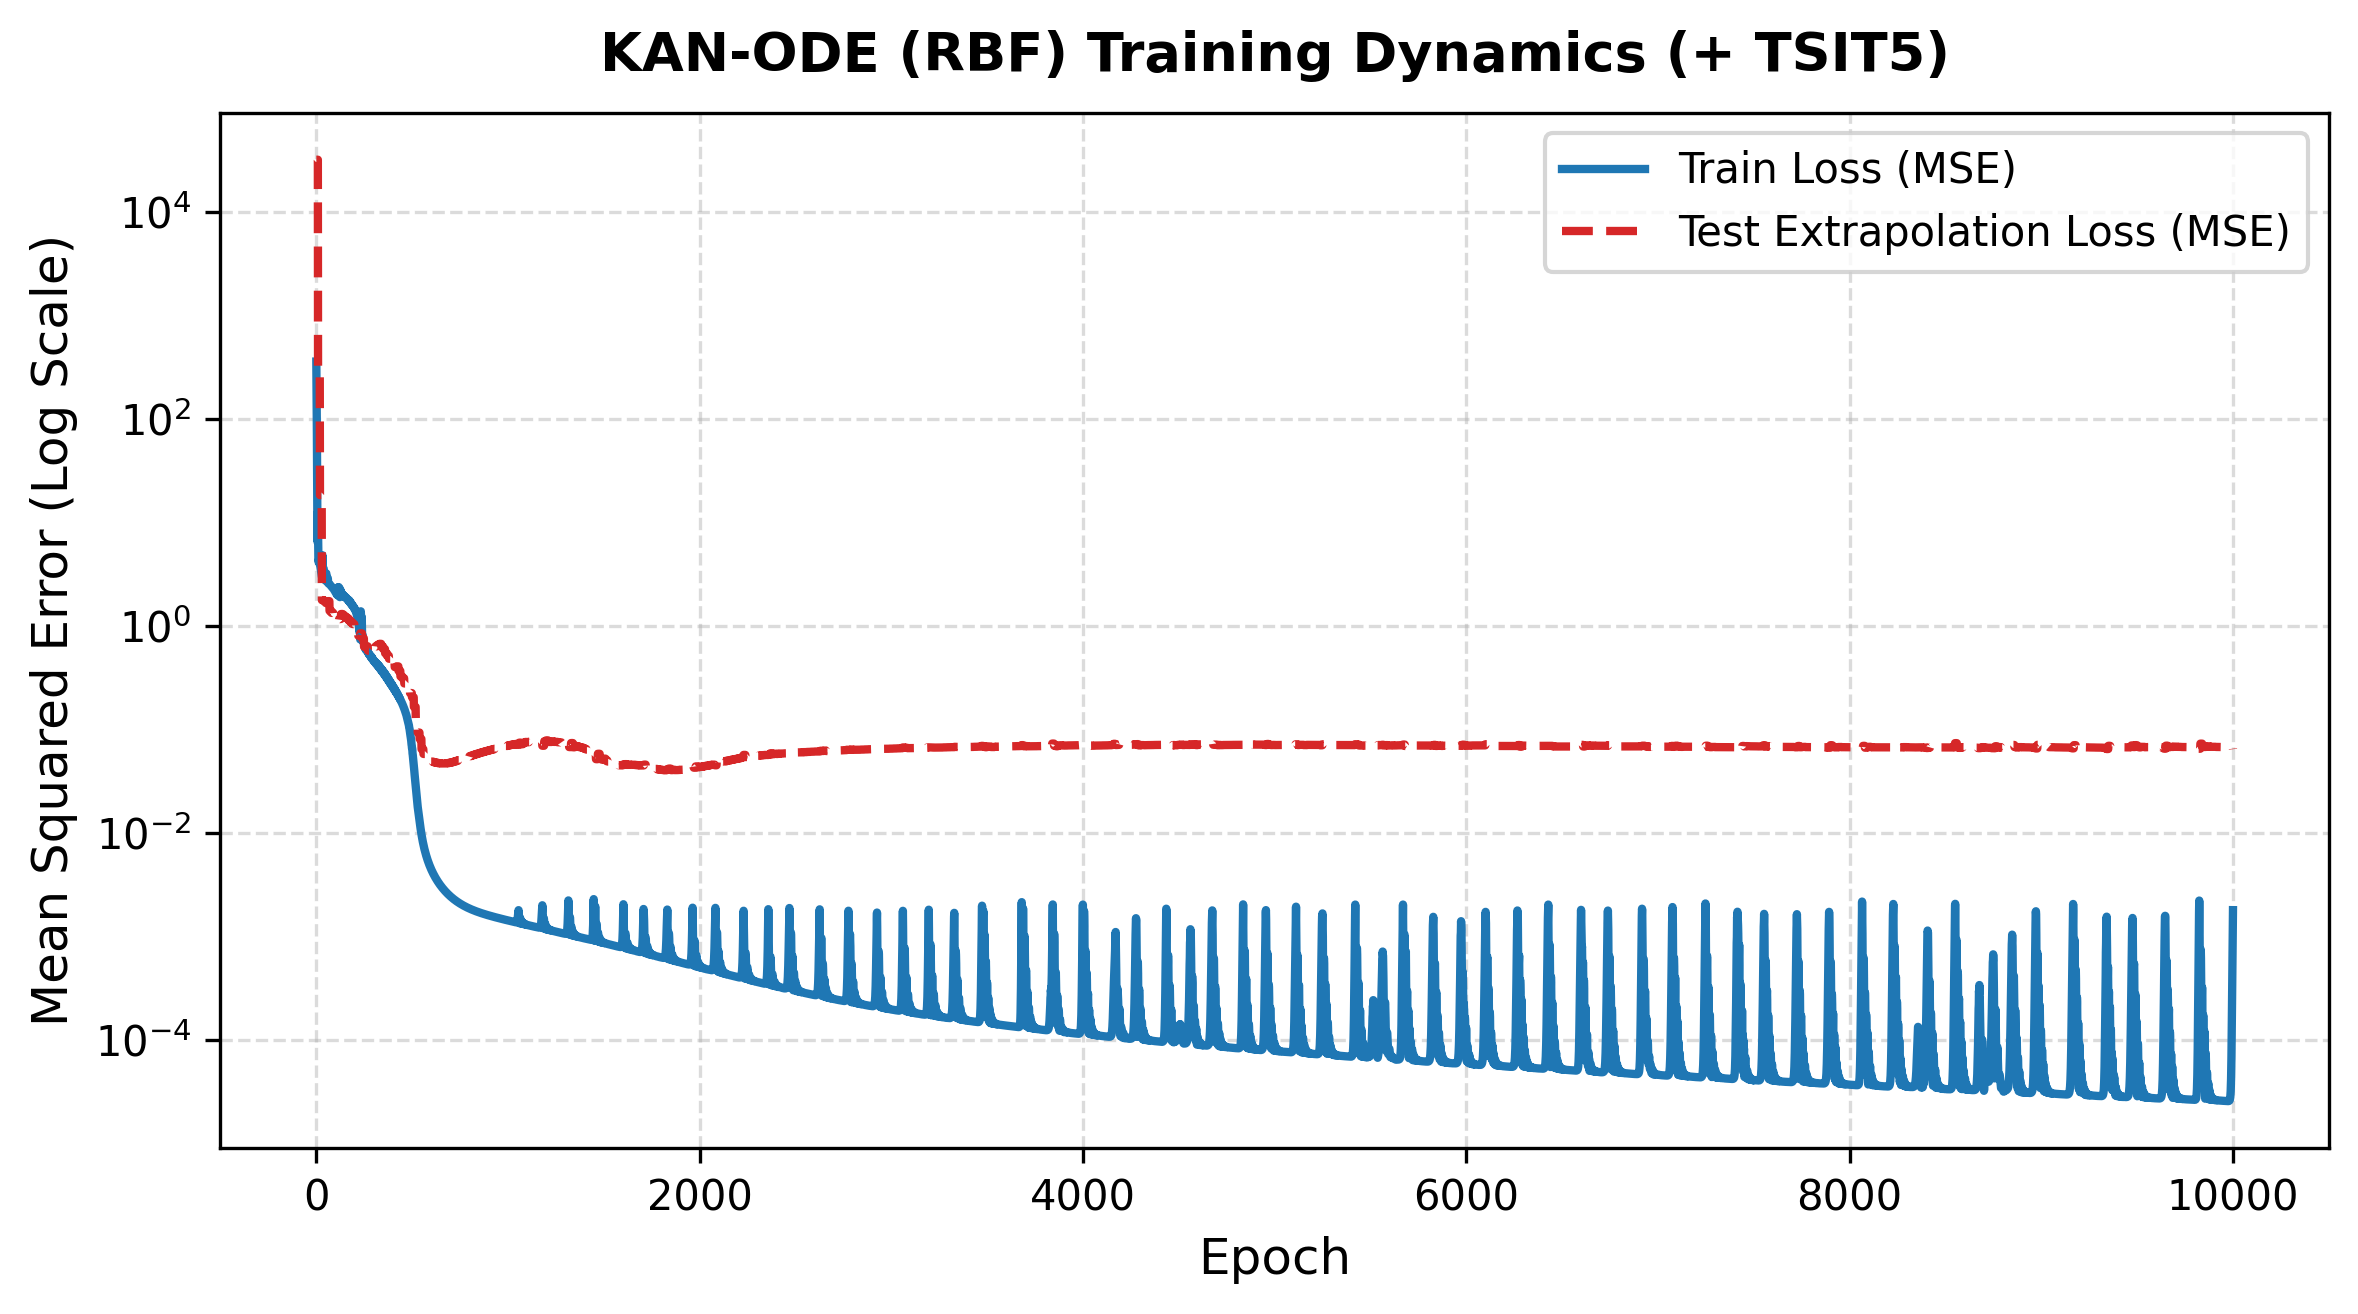
\includegraphics[width=\linewidth]{figures/phase2/pendulum_fixed_loss_curves.png}
\end{minipage}
\caption{Fixed-pendulum trajectory reconstruction (left) and training/extrapolation
loss curves (right), using the extended-window recipe.}
\label{fig:pendulum-fixed}
\end{figure*}

\paragraph{SIR: a unit-scale mismatch.} SIR diverged to an invalid
(not-a-number) value at epoch 8686.

\begin{expectbox}
\expectrow{Question}{What causes SIR's divergence, and is it a scale problem, an optimizer defect, or a modeling gap?}
\expectrow{Expected}{Measuring the untrained network's own field magnitude against the true dynamics, before any training, should reveal whether the two are mismatched in scale.}
\expectrow{Observed}{A $19\times$ speed mismatch at initialization. Rescaling time removes the divergence entirely; no optimizer or architecture change was needed.}
\end{expectbox}

Measuring the learned field magnitude \emph{before any training step}
explained the divergence directly. A Glorot-initialised KAN starts with
$|f_\theta|\approx0.203$, against SIR's true field magnitude of $0.011$: a
$19\times$ speed mismatch. To see why this is catastrophic rather than merely
inaccurate, note that backpropagation through an explicit solver
differentiates roughly $T/\Delta t$ nested nonlinear steps, and the resulting
gradient sensitivity grows exponentially as $e^{\Ltrunc \Ttrain}$, where
$\Ltrunc$ is the Lipschitz constant of $\mathbf{f}_\theta$ and $\Ttrain$ is
the integration horizon. Lotka-Volterra trains at $\Ttrain=3.5$ with
$|f|\sim10^0$ and converges. The pendulum trains at $\Ttrain=5.0$ with
$|f|\sim10^0$ and converges after the window fix. SIR sits at $\Ttrain=50$
with $|f|\sim10^{-2}$. There the product $\Ltrunc\Ttrain$ is large enough
that training actually fails at the gradient overflow recorded at epoch 11,
not at the later epoch 8686.

The optimizer was behaving rationally. With an epoch-0 loss of
$3.16\times10^{2}$, collapsing the field to $\mathbf{f}_\theta\to\mathbf{0}$
reduces the loss to $\approx10^{-1}$, a $3{,}000\times$ improvement
reachable immediately. SIR's natural timescale is the recovery period
$1/\gamma=10$~days. Substituting $\tau=t/10$ gives
$\dd\mathbf{y}/\dd\tau = 10\,\mathbf{f}(\mathbf{y})$ over
$\tau\in[0,5]$, which puts SIR in the same regime the other two systems
already train in. A separate mass-drift symptom is fixed by projecting the
learned field onto the zero-sum subspace,
$f_{\text{proj}}(\mathbf{y}) = f(\mathbf{y})-\tfrac{1}{n}\sum_i f_i(\mathbf{y})$.
This enforces the SIR invariant (Equation~\ref{eq:sir}) as a property of the
flow rather than as a penalty on the fit. A third fix, a
\emph{vanishing-field gate}, multiplies the learned field by the infected
fraction $I$, so that $I=0$ is a manifold of equilibria exactly as in
Equation~\ref{eq:sir}, where every term carries a factor of $I$. Unlike the
first two fixes, this one assumes something about the physics.
Table~\ref{tab:sir-fix-summary} therefore reports the first two fixes on
their own and then with the gate added. Rescaling and projection alone remove
the divergence and cut extrapolation RMSE by $4.4\times$. The gate gives a
further $25\times$, and only the full recipe reaches a high extrapolation
$R^2$. Over this window the true signal varies very little (standard
deviation $0.002$--$0.017$), so $R^2$ is harsh and RMSE is the more
informative number.

\begin{table}[t]
\centering
\footnotesize
\setlength{\tabcolsep}{3pt}
\renewcommand{\arraystretch}{1.15}
\caption{SIR before and after the fixes, at the full 10{,}000-epoch budget.
``Rescale + project'' applies time rescaling and the conservation
projection, which assume nothing beyond Equation~\ref{eq:sir}; ``+ gate''
adds the vanishing-field gate. Mass error is $\max_t|S+I+R-1|$.}
\label{tab:sir-fix-summary}
\begin{tabular}{@{}L{2.5cm} C{1.65cm} C{1.75cm} C{1.65cm}@{}}
\toprule
\hdrrow \thh{Metric} & \thh{Before fix} & \thh{Rescale + project} & \thh{+ gate}\\
\midrule
Training MSE & $4.39\times10^{-4}$ & $1.08\times10^{-5}$ & $\mathbf{2.28\times10^{-8}}$\\
Extrapolation RMSE & $0.0614$ & $0.0140$ & $\mathbf{5.7\times10^{-4}}$\\
Mass error & $0.0045$ & $\mathbf{0.0000}$ & $\mathbf{0.0000}$\\
Extrapolation $R^2$ & $-20.97$ & $-0.145$ & $\mathbf{+0.9981}$\\
Max.\ gradient norm & $5.82\times10^{18}$ & $92.3$ & $\mathbf{1.19}$\\
Final model & NaN (epoch 8686) & finite & finite\\
\bottomrule
\end{tabular}
\end{table}

\begin{figure*}[t]
\centering
\begin{minipage}[t]{0.48\textwidth}
\centering
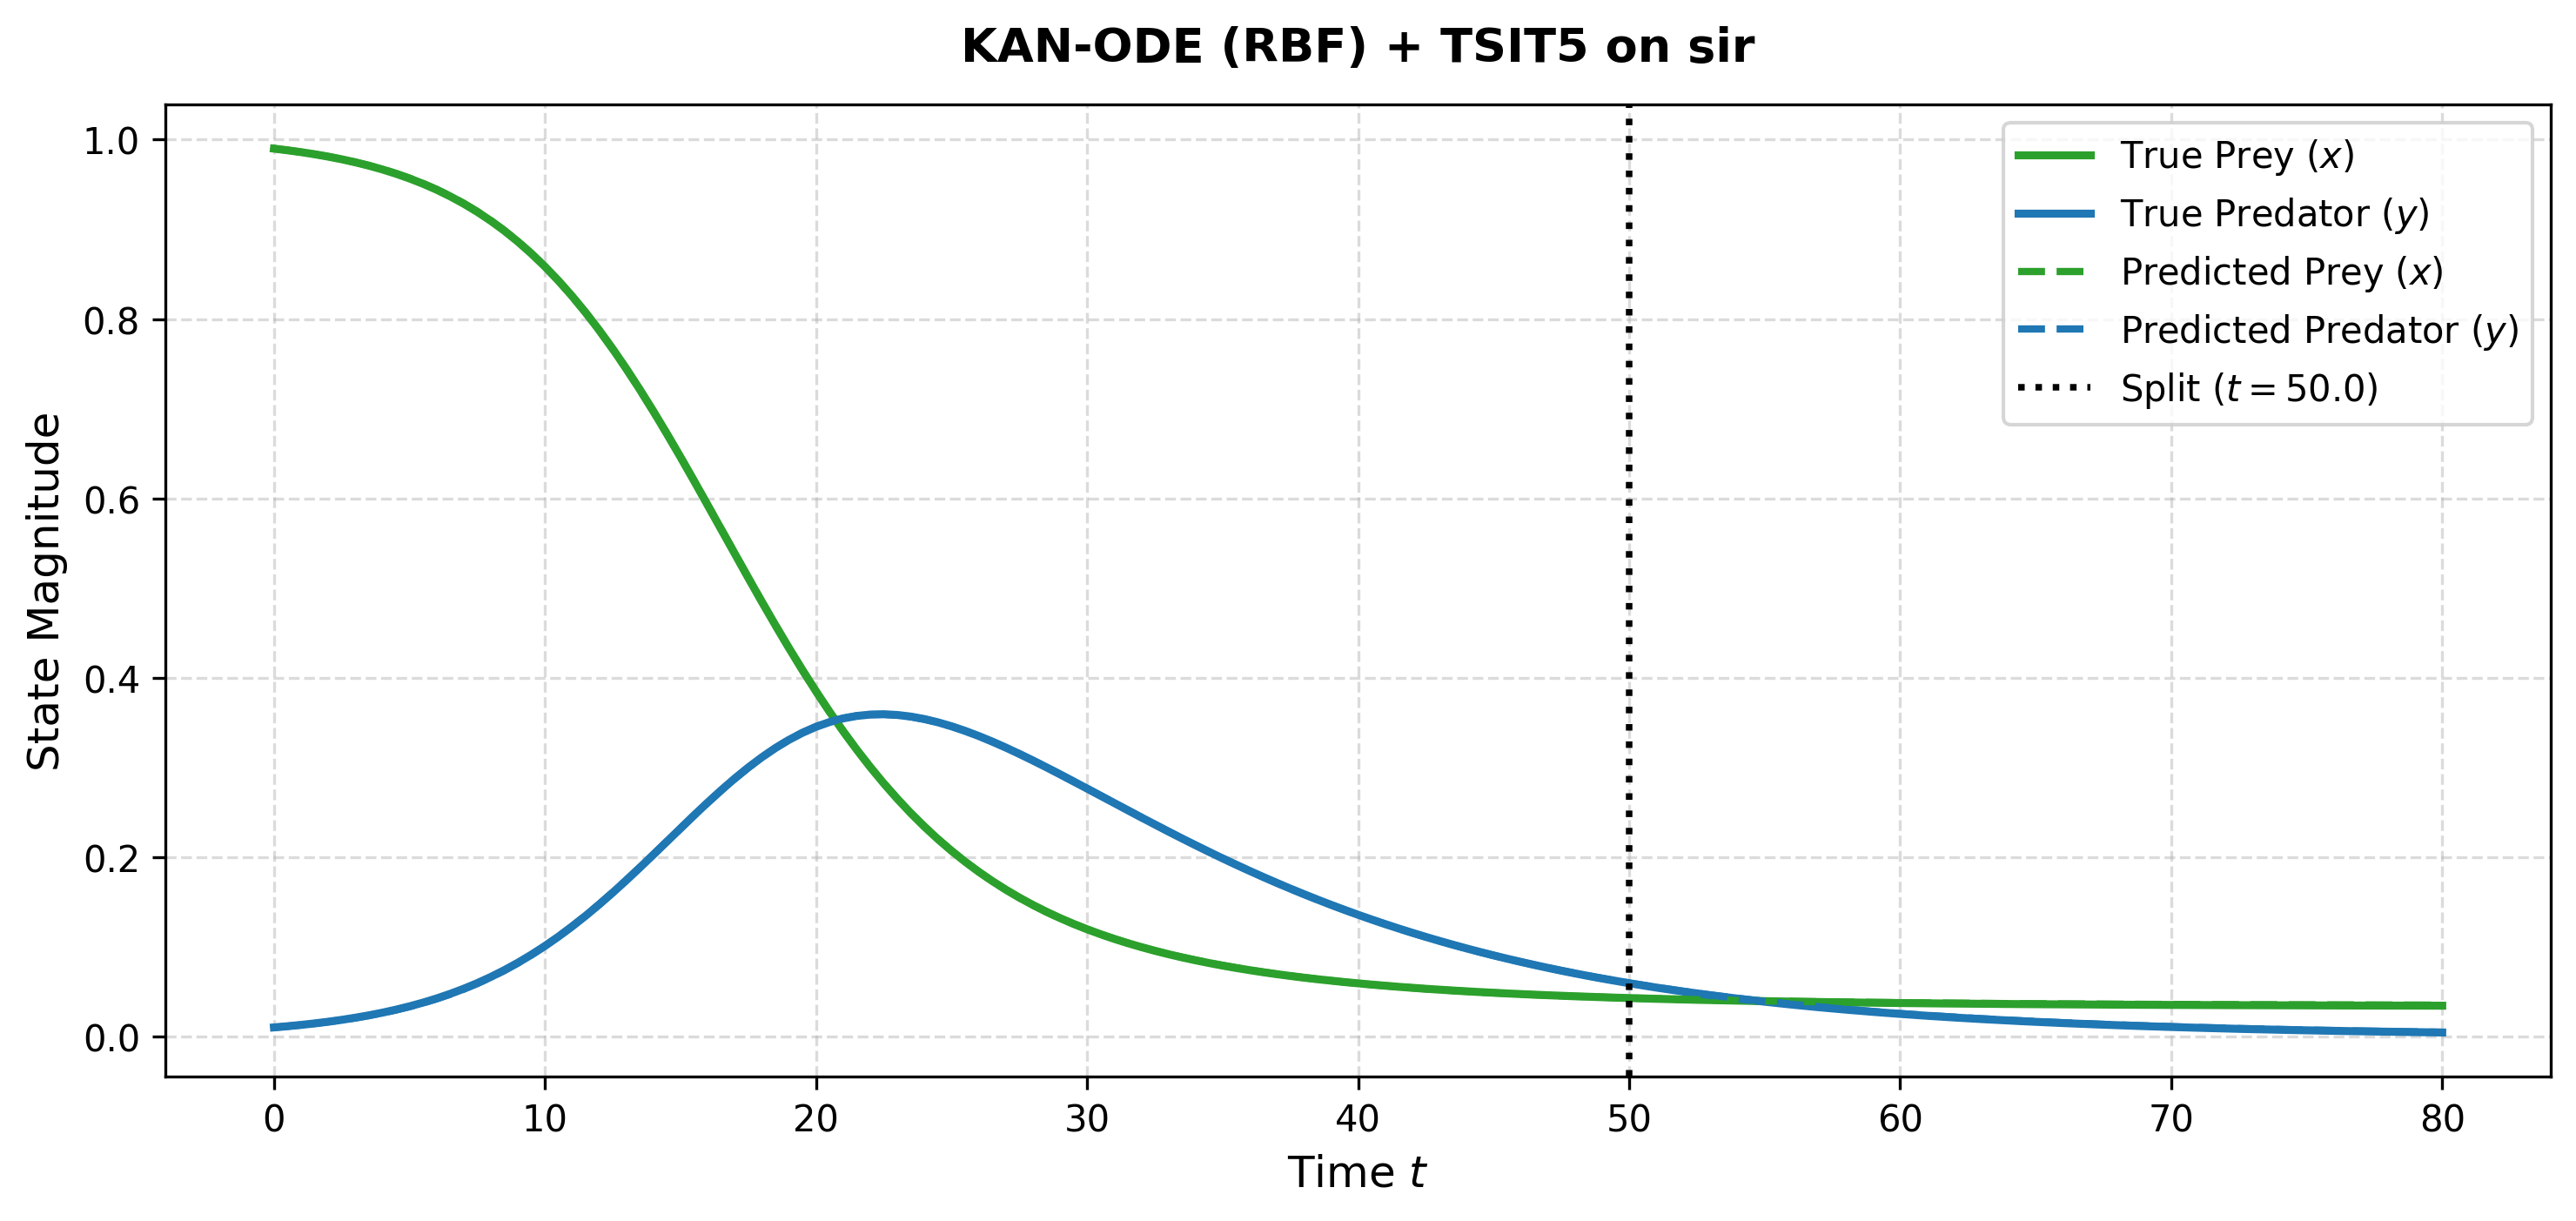
\includegraphics[width=\linewidth]{figures/phase2/sir_fixed_trajectory.png}
\end{minipage}\hfill
\begin{minipage}[t]{0.48\textwidth}
\centering
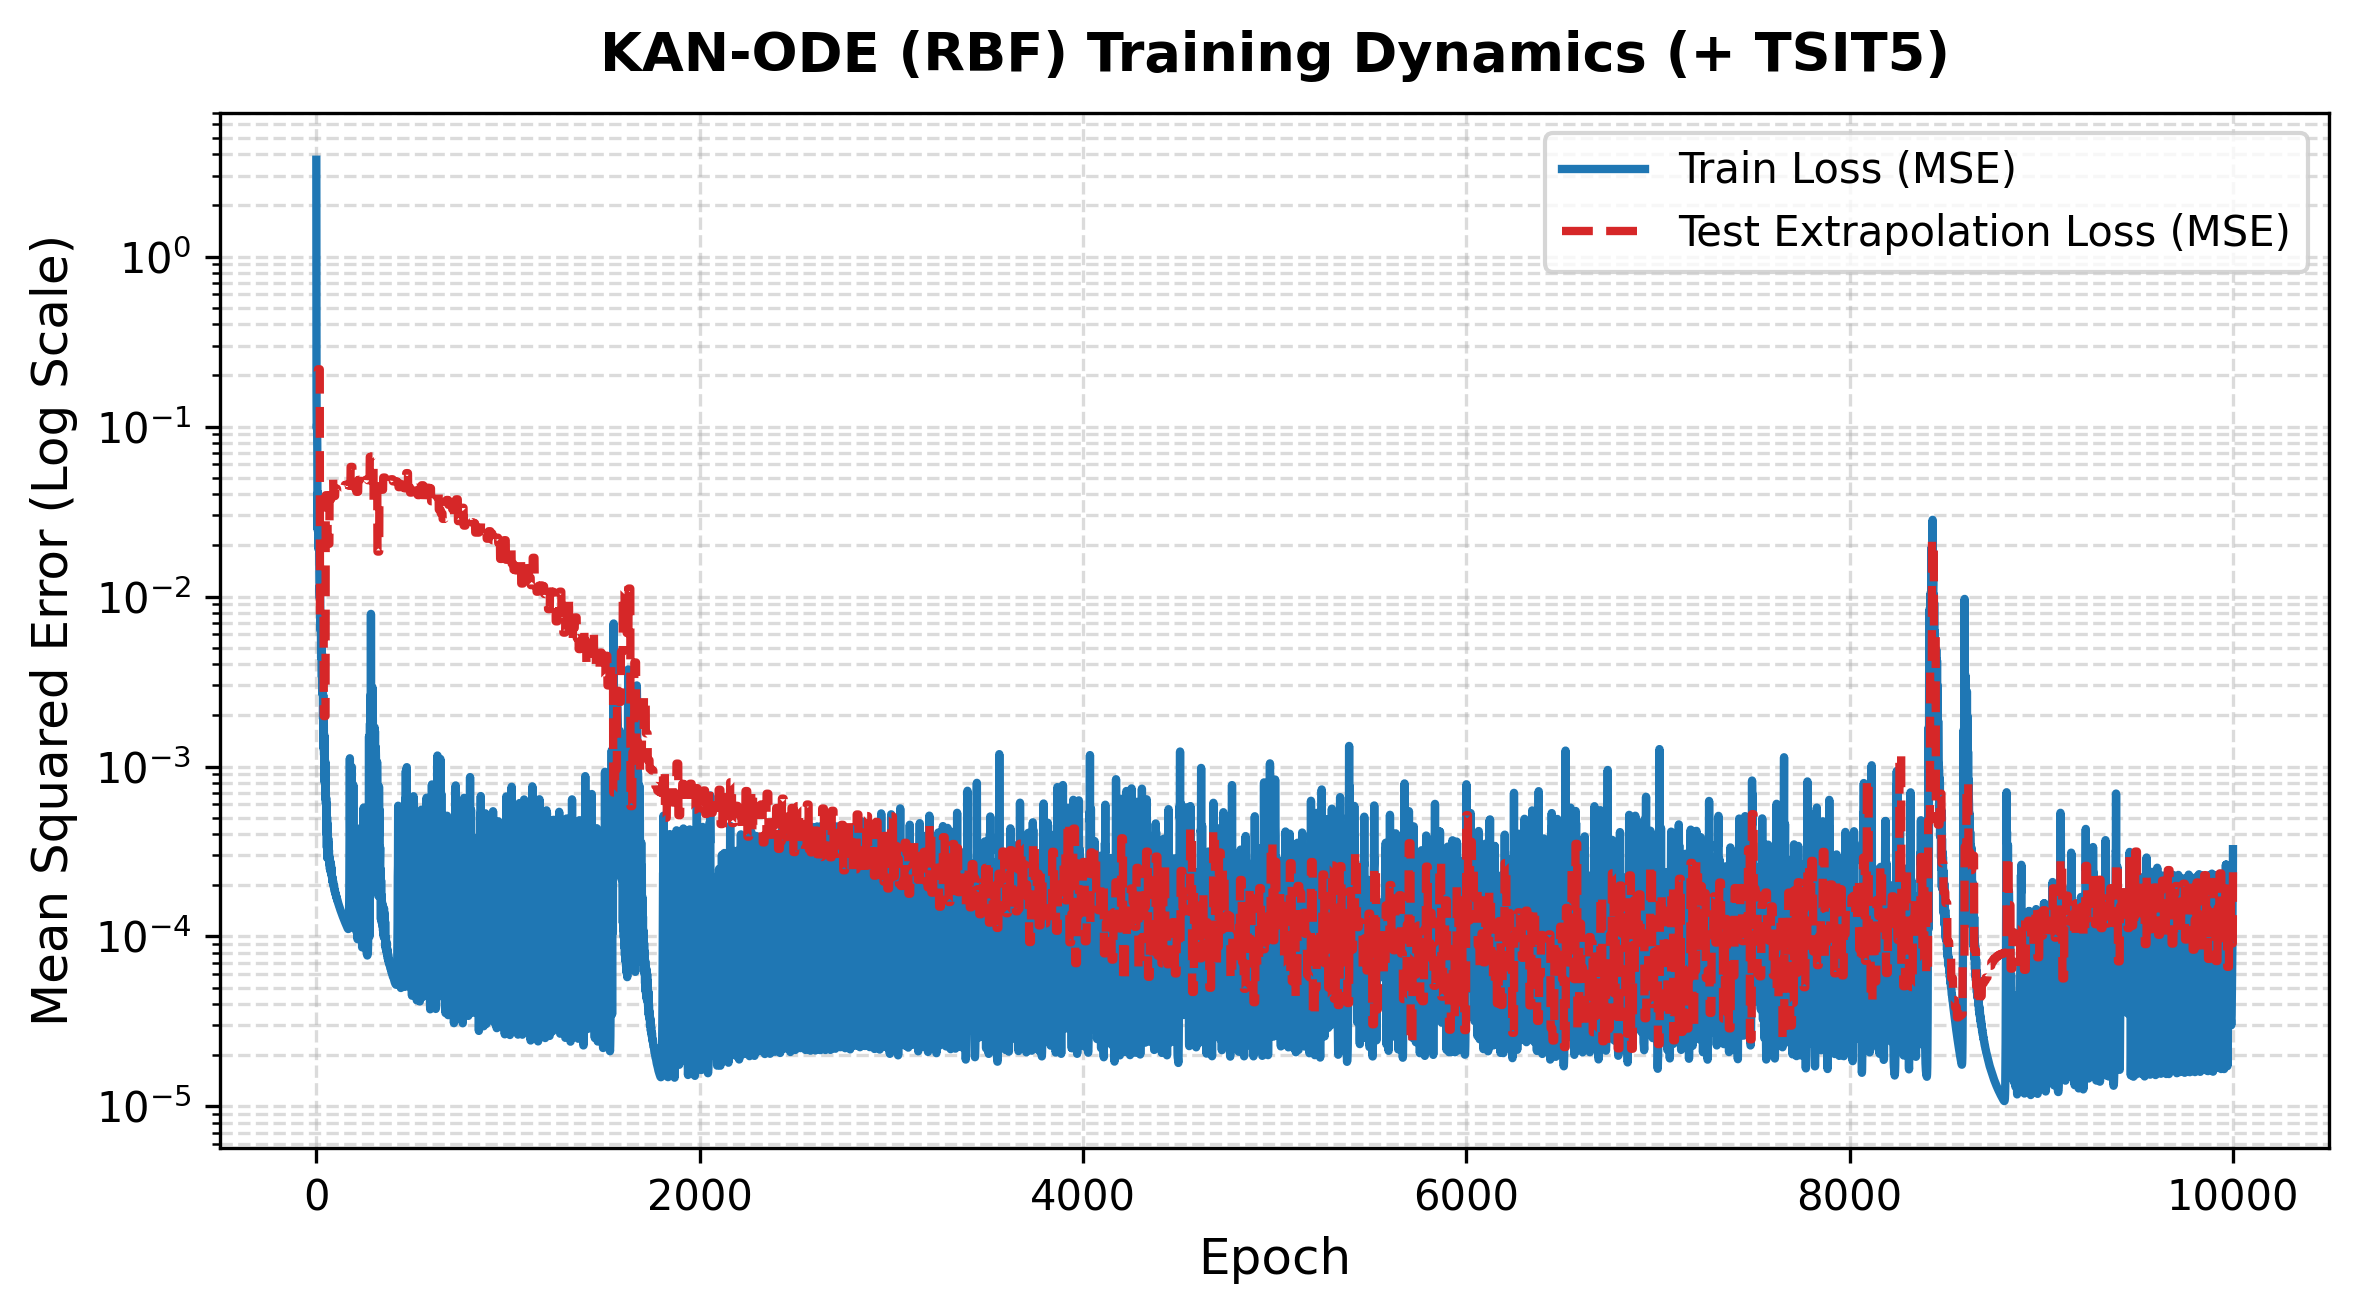
\includegraphics[width=\linewidth]{figures/phase2/sir_fixed_loss_curves.png}
\end{minipage}
\caption{SIR with all three fixes: reconstruction of $S$ and $I$ over the
full horizon (left; the plot's generic legend labels them prey and predator)
tracks the true dynamics closely;
training and extrapolation loss curves (right) decrease together without
the gradient overflow that terminated the original run.}
\label{fig:sir-fixed}
\end{figure*}

\paragraph{Other fixes considered.} We tested several more interventions.
Table~\ref{tab:fix-scorecard} records them for completeness, including those
we did not adopt.

\begin{table*}[t]
\centering
\footnotesize
\renewcommand{\arraystretch}{1.15}
\caption{Every stability intervention tested, including the rejected ones.}
\label{tab:fix-scorecard}
\begin{tabularx}{\textwidth}{@{}L{5.0cm} C{2.4cm} Y@{}}
\toprule
\hdrrow \thh{Intervention} & \thh{Verdict} & \thh{Evidence}\\
\midrule
Longer training window (pendulum) & Adopted & $R^2$ improves from $-1.318$ to $+0.647$; works for both activations tested\\
Non-finite gradient guard with automatic abort & Adopted & Caught the divergence of an intermediate SIR recipe (conservation penalty plus loss weighting) at epoch 3055 and preserved a valid checkpoint instead of overwriting it with an invalid one\\
Time rescaling (SIR) & Adopted & Removes both the divergence and the frozen-field behavior\\
Conservation via subspace projection (SIR) & Adopted & Mass error reduced from $4.5\times10^{-3}$ to $0.0000$ (exact by construction)\\
Vanishing-field gate (SIR) & Adopted & Extrapolation RMSE reduced a further $25\times$ ($0.0140\to5.7\times10^{-4}$); the only fix that assumes a physical property\\
Identity activation (pendulum) & Speed only & Roughly $1000\times$ faster to fit at the short window, but worse extrapolation and stability at the long window\\
Standard-deviation loss weighting & System-dependent & Worst-performing pendulum option; superseded for SIR by time rescaling\\
Conservation via penalty term & Rejected & Wrong mechanism: the training window's mass was already close to conserved, so the penalty had nothing to correct (mass error still $0.0086$)\\
Widened basis-function grid limits & Rejected & Performed worse than the untouched baseline configuration\\
\bottomrule
\end{tabularx}
\end{table*}

\begin{keypoint}[Methodological lesson carried into every later study]
Both diagnoses came from measuring the learned field's own magnitude at
initialization, before training ever ran. The same init-time measurement
reappears verbatim in the epidemic-curve test of
Section~\ref{sec:track-e}.
\end{keypoint}

\subsubsection{Extended extrapolation: the KAN advantage widens with horizon}

With the fixes in place, we extended the Lotka-Volterra extrapolation
horizon from four periods ($t\in(3.5,14]$) to eight periods
($t\in(3.5,28]$), using the same trained model with no retraining.

\begin{table*}[t]
\centering
\footnotesize
\renewcommand{\arraystretch}{1.15}
\caption{Extrapolation MSE as the horizon doubles, same trained models.}
\label{tab:extrap-horizon}
\begin{tabular}{@{}L{4.6cm} C{2.6cm} C{3.3cm} C{3.3cm} C{2.2cm}@{}}
\toprule
\hdrrow \thh{Model} & \thh{Training $[0,3.5]$} & \thh{Near extrapolation $(3.5,14]$} & \thh{Far extrapolation $(14,28]$} & \thh{Degradation}\\
\midrule
\textbf{KAN-ODE} (RBF, 240 parameters) & $8.83\times10^{-5}$ & $8.92\times10^{-5}$ & $\mathbf{9.72\times10^{-5}}$ & $\mathbf{1.1\times}$\\
MLP-ODE (SiLU, 252 parameters) & $9.50\times10^{-5}$ & $4.78\times10^{-4}$ & $3.95\times10^{-3}$ & $8.3\times$\\
MLP-ODE (tanh, paper lr/init, 252 parameters) & $1.11\times10^{-3}$ & $9.65\times10^{-3}$ & $5.95\times10^{-2}$ & $6.2\times$\\
\bottomrule
\end{tabular}
\end{table*}

The KAN-ODE's error is essentially flat across eight periods
($8.83\to8.92\to9.72\times10^{-5}$, a $10\%$ rise from the training window
to double the original horizon), while the parameter-matched MLP degrades
$8.3\times$ over the same extension. The KAN-ODE advantage therefore widens
with horizon, from $5.4\times$ at four periods to $\mathbf{40.6\times}$ at
eight. This is a materially stronger claim than the near-horizon comparison
presented earlier: KAN-ODE error does not accumulate, so the gap grows with
every additional period.

\subsubsection{Pendulum energy dissipation: an independent physical check}

The fixed pendulum recipe captures $94.2\%$ of the true energy dissipation
and tracks $E(t)$ to $0.6\%$ inside the training window. However, the strict
monotonic-decay invariant ($\dd E/\dd t\le0$, Equation~\ref{eq:pendulum})
is violated on 40 of 200 predicted steps. The model is under-damped: the
true angular displacement decays to $0.004$ by $t=9.1$, while the predicted
trajectory keeps oscillating at $0.237$. This energy diagnostic independently
confirms the under-damping, expressed as a violated conservation law rather
than a trajectory RMSE (Figure~\ref{fig:pendulum-energy}).

\begin{figure*}[t]
\centering
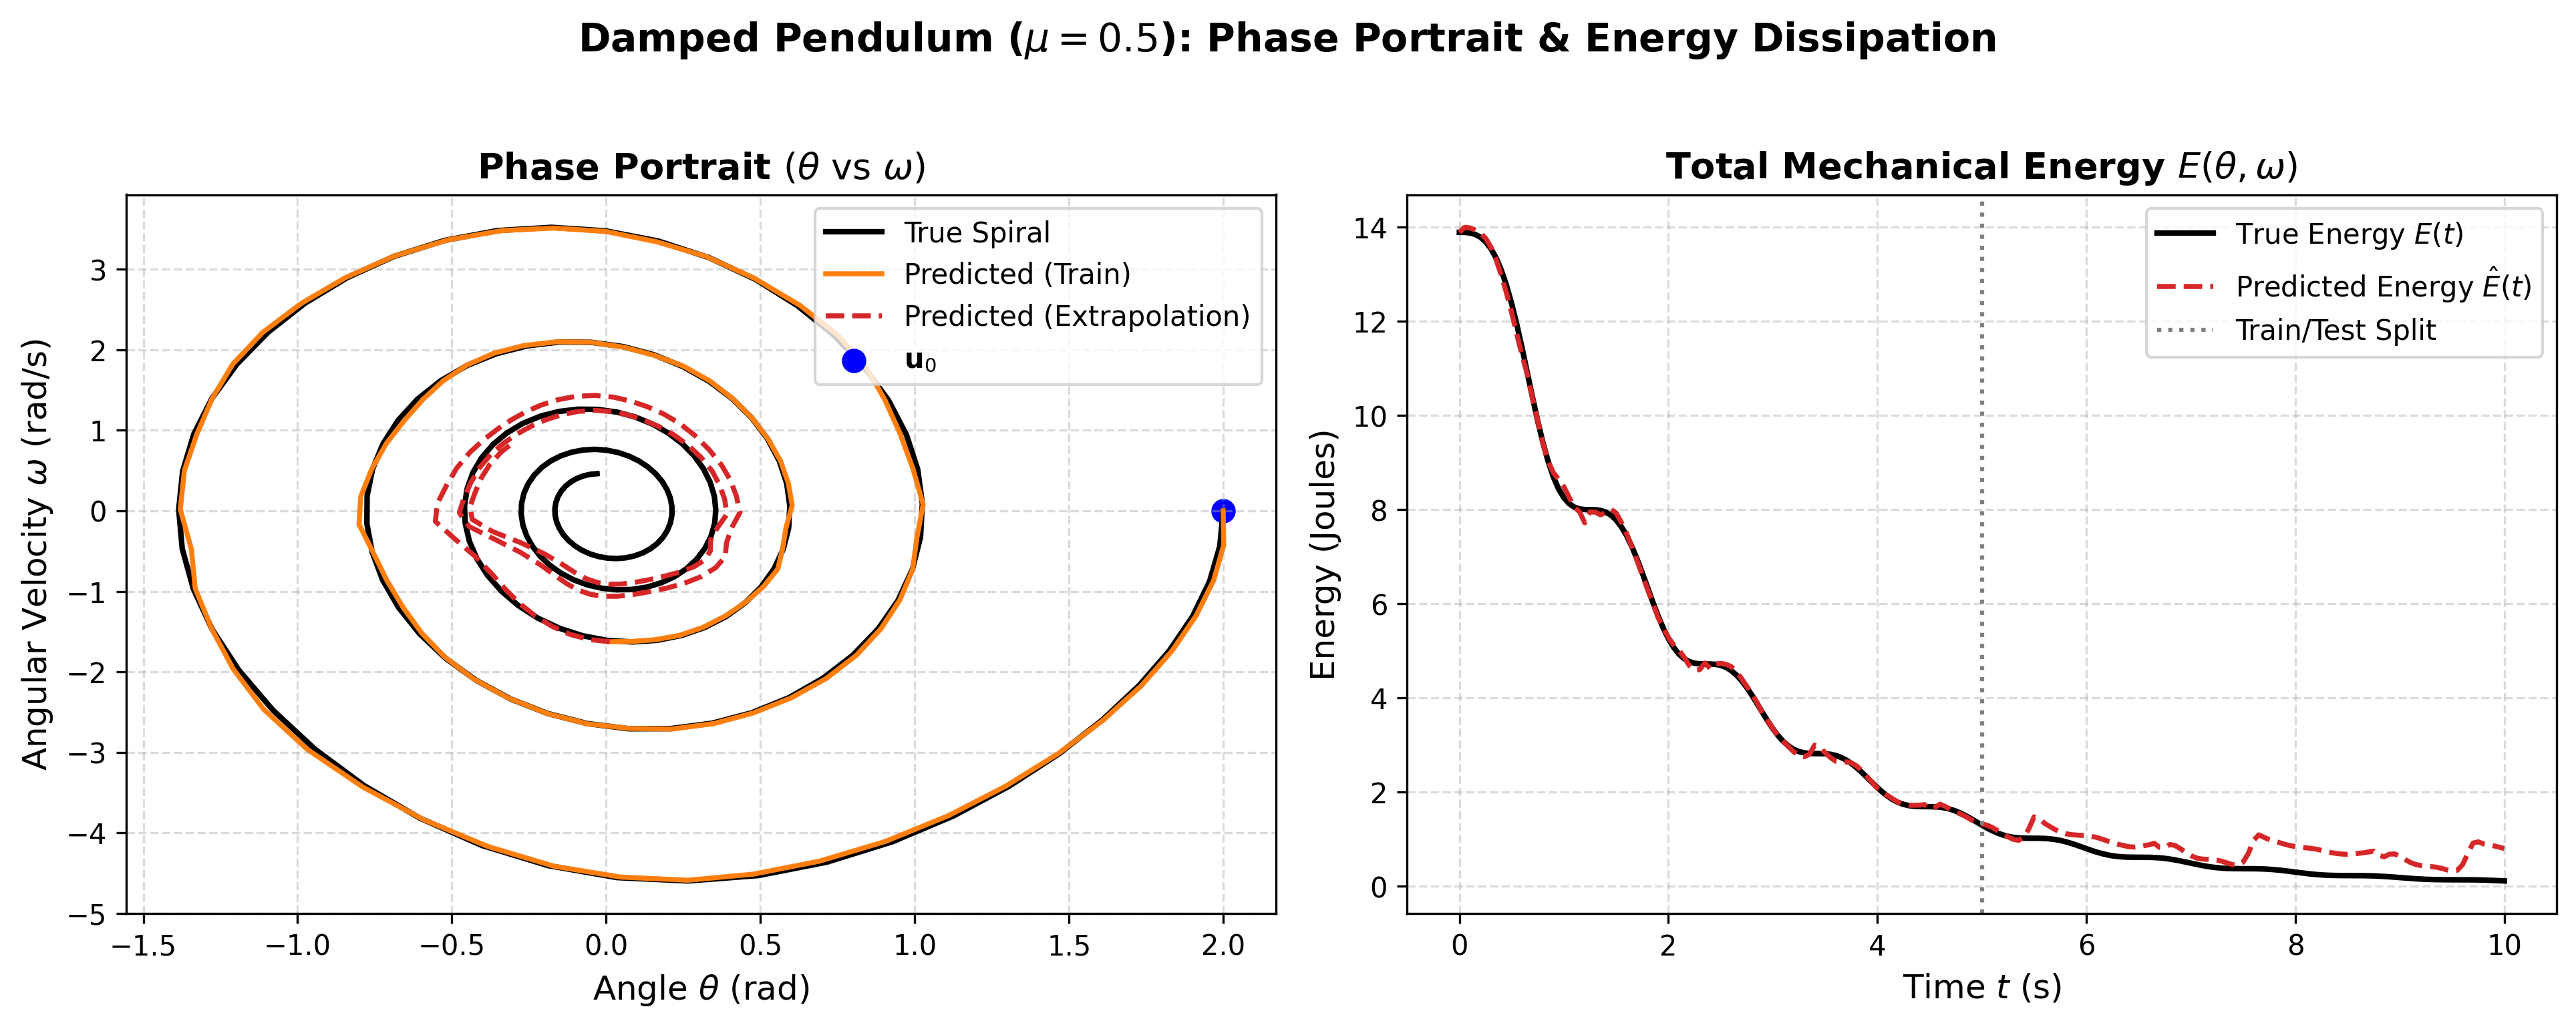
\includegraphics[width=0.9\textwidth]{figures/phase2/pendulum_energy.png}
\caption{Fixed pendulum ($\mu=0.5$, $t_{\text{train}}=5$): phase portrait
(left) and total mechanical energy $E(\theta,\omega)$ (right). Inside the
training window the predicted energy follows the true curve closely; past the
split at $t=5$ it stays above the truth and rises on 40 of 200 predicted
steps, the under-damping described in the text.}
\label{fig:pendulum-energy}
\end{figure*}

\subsection{Adjoint sensitivity vs.\ direct autograd}
\label{sec:track-a}

Our own implementation documentation adopted direct autograd on the grounds
that the adjoint method's $O(1)$ memory advantage
(Section~\ref{sec:gradients}) does not matter for our short trajectories
($N_t\in[36,101]$). We test that claim directly on an RTX~3060. The
integrator is held fixed (classical RK4 at matched step size on both paths),
and a forward-trajectory check confirms the two implementations agree to
$\sim10^{-7}$ relative error, so only the differentiation method varies.

\begin{expectbox}
\expectrow{Question}{Does adjoint sensitivity's constant memory cost make it the better choice at our trajectory lengths, as our own documentation assumes?}
\expectrow{Expected}{Direct autograd should be cheaper in memory at these short lengths, with adjoint's advantage only appearing once trajectories grow much longer.}
\expectrow{Observed}{Adjoint already uses less memory at every length tested. The deciding cost is wall-clock, not memory: adjoint is $1.9$--$2.1\times$ slower.}
\end{expectbox}

\begin{table*}[t]
\centering
\small
\renewcommand{\arraystretch}{1.15}
\caption{Peak VRAM and wall-clock, direct autograd vs.\ adjoint sensitivity.}
\label{tab:adjoint-profiling}
\begin{tabularx}{\textwidth}{@{}X C{2.8cm} L{3.4cm} C{2.8cm} C{3.2cm}@{}}
\toprule
\hdrrow \thh{System} & \thh{Trajectory length $N_t$} & \thh{Method} & \thh{Peak VRAM (MB)} & \thh{Seconds per 1000 epochs}\\
\midrule
Lotka-Volterra & 36 & Direct autograd & 18.61 & 317.5\\
Lotka-Volterra & 36 & Adjoint & 17.08 & 672.9\\
SIR & 101 & Direct autograd & 21.52 & 984.8\\
SIR & 101 & Adjoint & 17.12 & 1871.6\\
\bottomrule
\end{tabularx}
\end{table*}

\begin{figure}[tb]
\centering
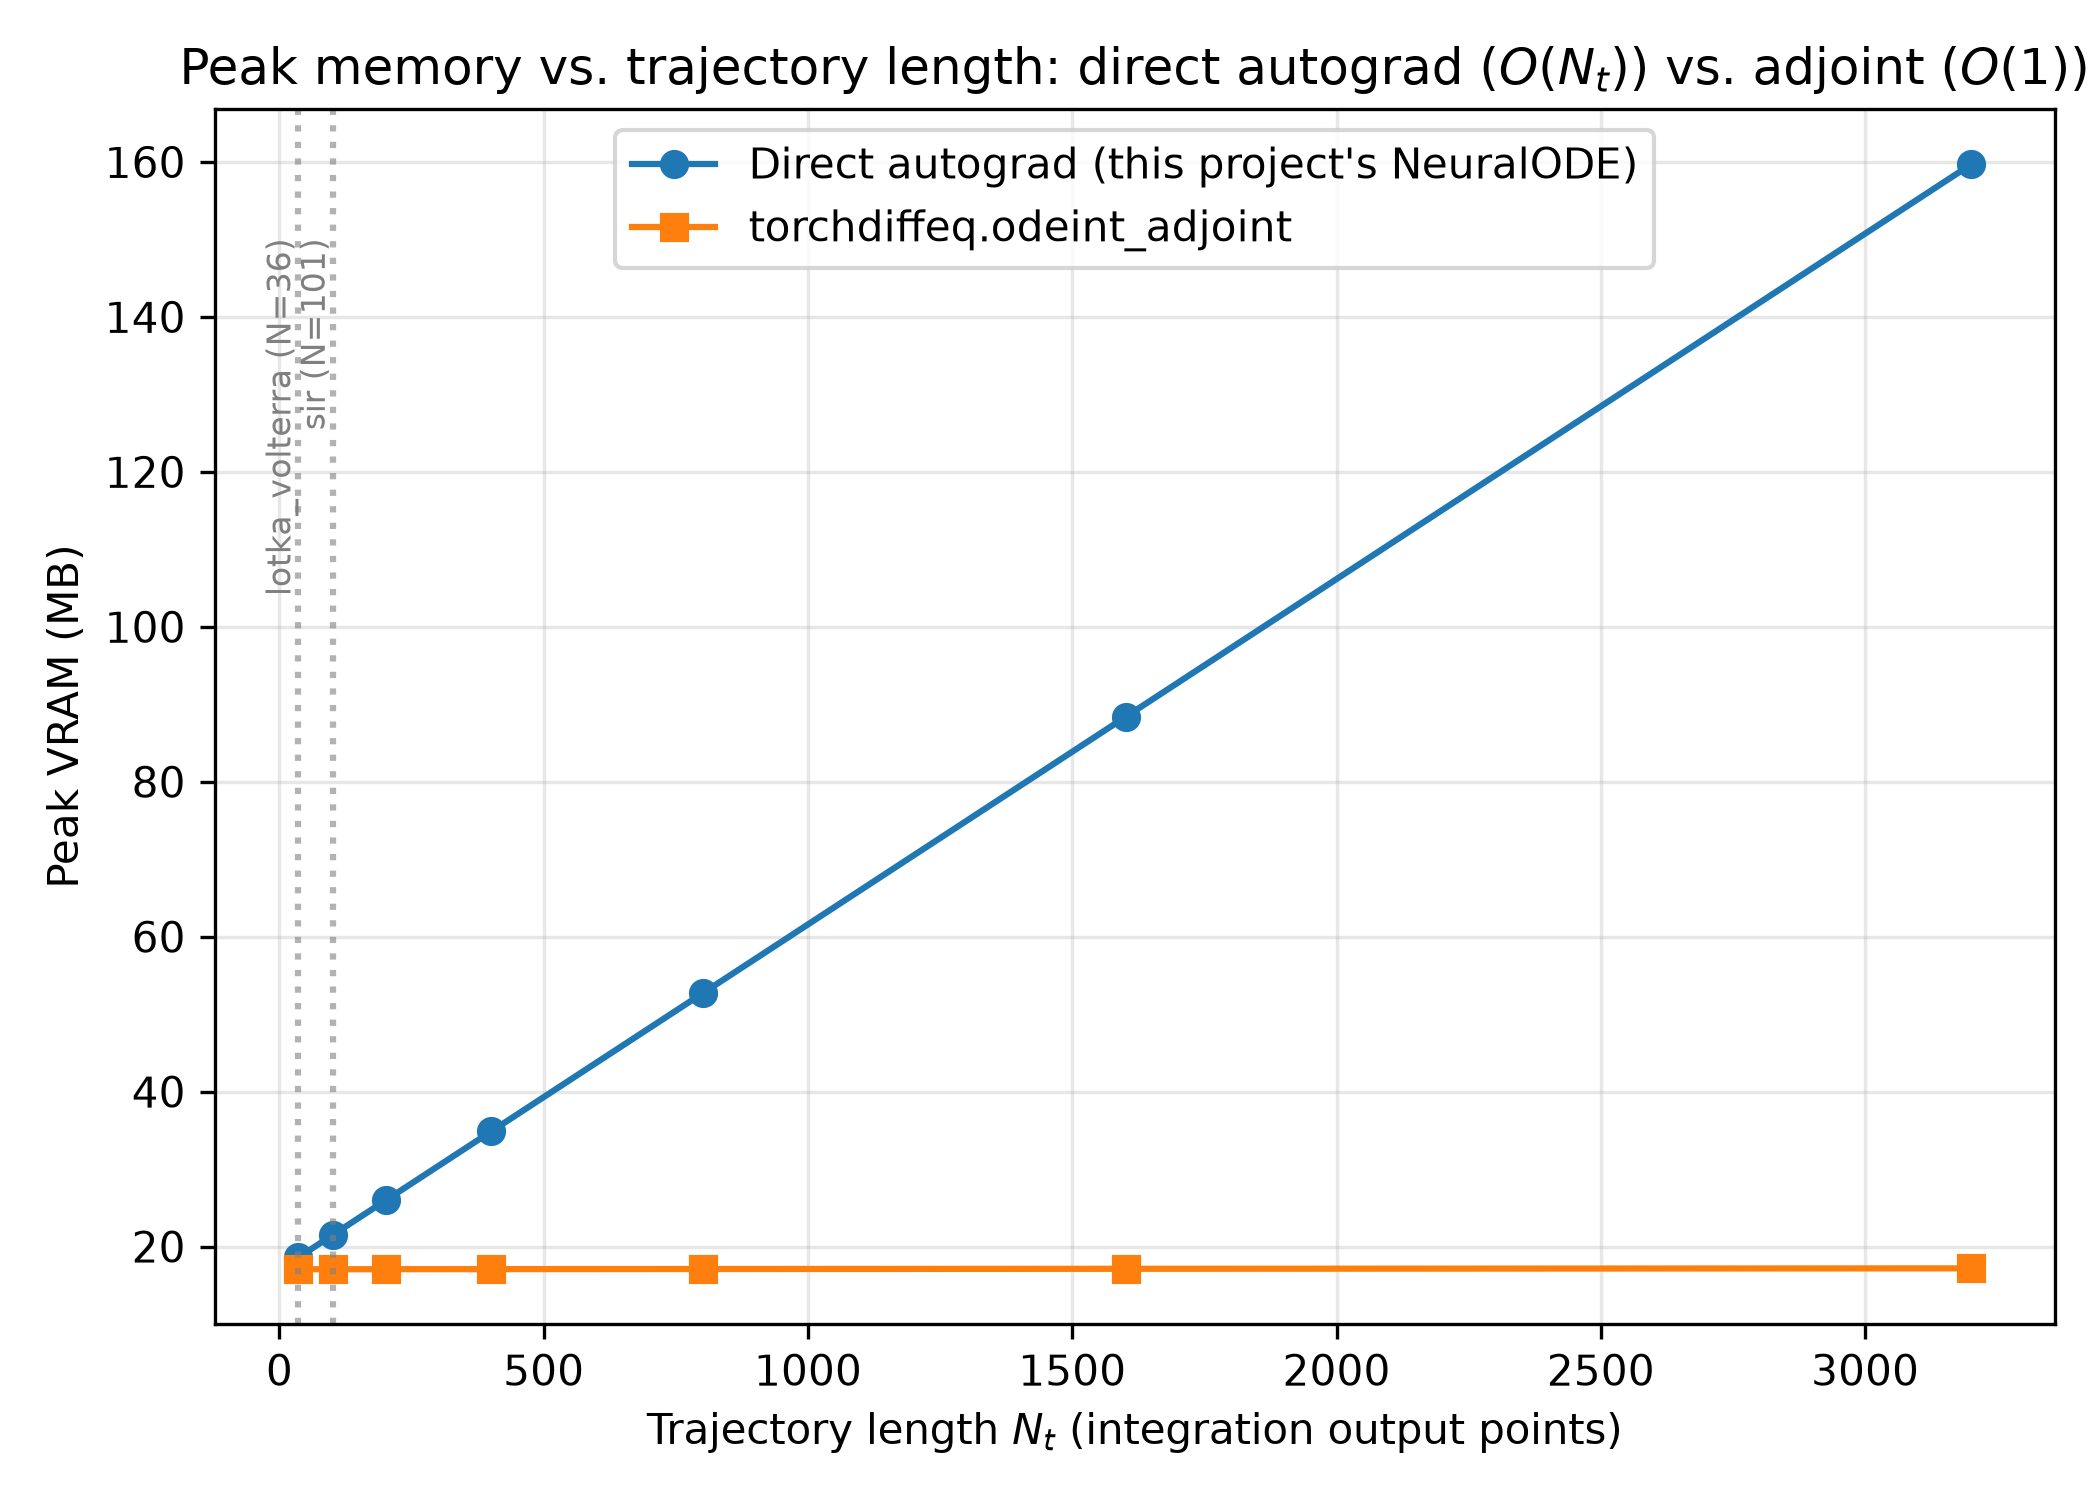
\includegraphics[width=\columnwidth]{figures/track_a/memory_vs_trajectory_length.png}
\caption{Peak memory vs.\ trajectory length $N_t\in\{36,\dots,3201\}$: direct
autograd grows linearly ($\approx0.045$~MB per output point); adjoint stays
flat (0.7\% increase over an $89\times$ length increase).}
\label{fig:adjoint-memory}
\end{figure}

\paragraph{Finding.} The measured memory data contradicts the premise behind
the original choice, but still supports its conclusion. The $O(N_t)$ vs.\
$O(1)$ scaling in Equation~\ref{eq:adjoint} predicts a crossover length below
which direct autograd should still win on raw memory, because it avoids the
adjoint method's own bookkeeping overhead. The data shows no such crossover
inside the tested range. Adjoint uses \emph{less} memory than direct autograd
at every tested length, including the shortest ($N_t=36$: $17.08$ vs.\
$18.61$~MB). As Figure~\ref{fig:adjoint-memory} shows, direct autograd's
per-step storage cost is already large enough at our scale to outweigh
whatever constant overhead the adjoint bookkeeping carries.
Extrapolating the measured linear slope of direct autograd's memory growth,
$N_t$ would need to reach $\approx225{,}000$ before it threatens a 12~GB
card. For us the deciding factor is wall-clock: solving the continuous
adjoint ODE backward in time costs a consistent $1.9$--$2.1\times$ overhead
at both tested lengths. That turns a 53-minute Lotka-Volterra run into
$\sim$112~minutes, for a memory saving that never matters in practice (peak
usage is $0.17\%$ of card capacity). Gradient relative error is
$2.85\times10^{-7}$ and $4.88\times10^{-7}$ respectively, well inside a
$5\times10^{-3}$ tolerance. Both methods agree numerically, so the choice
reduces to a resource trade-off, and direct autograd is the faster option
for every dataset in our scope ($N_t\le201$).

\subsection{Gradient-norm dynamics}
\label{sec:track-b}

The benchmark ablation found Forward Euler uniquely unable to reach $10^{-4}$
training loss within budget, with $28\times$ worse extrapolation MSE than
Tsit5 (Table~\ref{tab:solver-ablation}). The candidate mechanism we test
here: a first-order solver commits $O(\Delta t)$ local error every step,
which could inject measurably noisier gradients and destabilize Adam's
moment estimates.

\begin{expectbox}
\expectrow{Question}{Does a lower-order solver's larger truncation error show up as measurably noisier gradients during training?}
\expectrow{Expected}{Gradient-norm noise should fall as solver order rises, correlating with the accuracy ranking already seen in the benchmark ablation.}
\expectrow{Observed}{No reliable correlation ($\rho=-0.088$, $p=0.87$); the ranking is non-monotone and its sign flips depending on an arbitrary warm-up cut. Refuted.}
\end{expectbox}

The noise measure is the standard deviation of epoch-to-epoch \emph{relative}
gradient change, which is scale-invariant by construction:
\begin{equation}
\begin{gathered}
\eta = \operatorname{std}\big(\Delta\log_{10} g\big), \\
\Delta\log_{10} g_i = \log_{10} g_{i+1} - \log_{10} g_i.
\end{gathered}
\label{eq:noise-measure}
\end{equation}
We compare $\eta$ against solver order $p$ using Spearman rank correlation
rather than the more familiar Pearson correlation. Pearson measures how
linearly two quantities move together. That presumes the numeric spacing of
solver order is meaningful, i.e.\ that the jump from order 1 to order 2 is
comparable in size to the jump from order 4 to order 5. There is no reason
to expect $\eta$ to depend on solver order that linearly. The hypothesis
under test is only that noise falls \emph{monotonically} as order rises,
which is exactly what Spearman correlation measures, since it compares ranks
rather than raw values. It also handles the deliberate tie at $p=2$ (Heun and
Midpoint are both second-order methods) natively, where Pearson would need
an arbitrary tie-breaking rule.

\begin{table*}[t]
\centering
\small
\renewcommand{\arraystretch}{1.15}
\caption{Gradient-noise measure $\eta$ vs.\ solver order, six solvers, $n=6$.}
\label{tab:gradient-noise}
\begin{tabularx}{\textwidth}{@{}L{3.4cm} C{2.2cm} C{2.6cm} C{3.4cm} X@{}}
\toprule
\hdrrow \thh{Solver} & \thh{Order $p$} & \thh{Noise $\eta$} & \thh{Best training MSE} & \thh{Noise rank}\\
\midrule
Forward Euler & 1 & $0.2805$ & $1.377\times10^{-4}$ & 1 (noisiest)\\
Classical RK4 & 4 & $0.2726$ & $9.413\times10^{-5}$ & 2\\
Tsit5 & 5 & $0.2683$ & $8.833\times10^{-5}$ & 3\\
DOPRI5 & 5 & $0.2660$ & $9.283\times10^{-5}$ & 4\\
Midpoint RK2 & 2 & $0.2634$ & $8.857\times10^{-5}$ & 5\\
Heun RK2 & 2 & $0.2621$ & $8.315\times10^{-5}$ & 6\\
\bottomrule
\end{tabularx}
\end{table*}

Spearman $\rho=-0.088$, $p=0.87$ ($n=6$). Three findings jointly refute the
hypothesis. First, the effect size is a 7\% spread across all six solvers.
Second, the ranking is non-monotone (RK4, order 4, is the second-noisiest
solver). Third, the sign of $\rho$ flips across warm-up cuts
($-0.088\to-0.441\to+0.706$ as the first 0, 2000, 5000 epochs are dropped),
so no cut reaches significance and the direction of any relationship depends
on an arbitrary analyst choice.

\begin{figure*}[t]
\centering
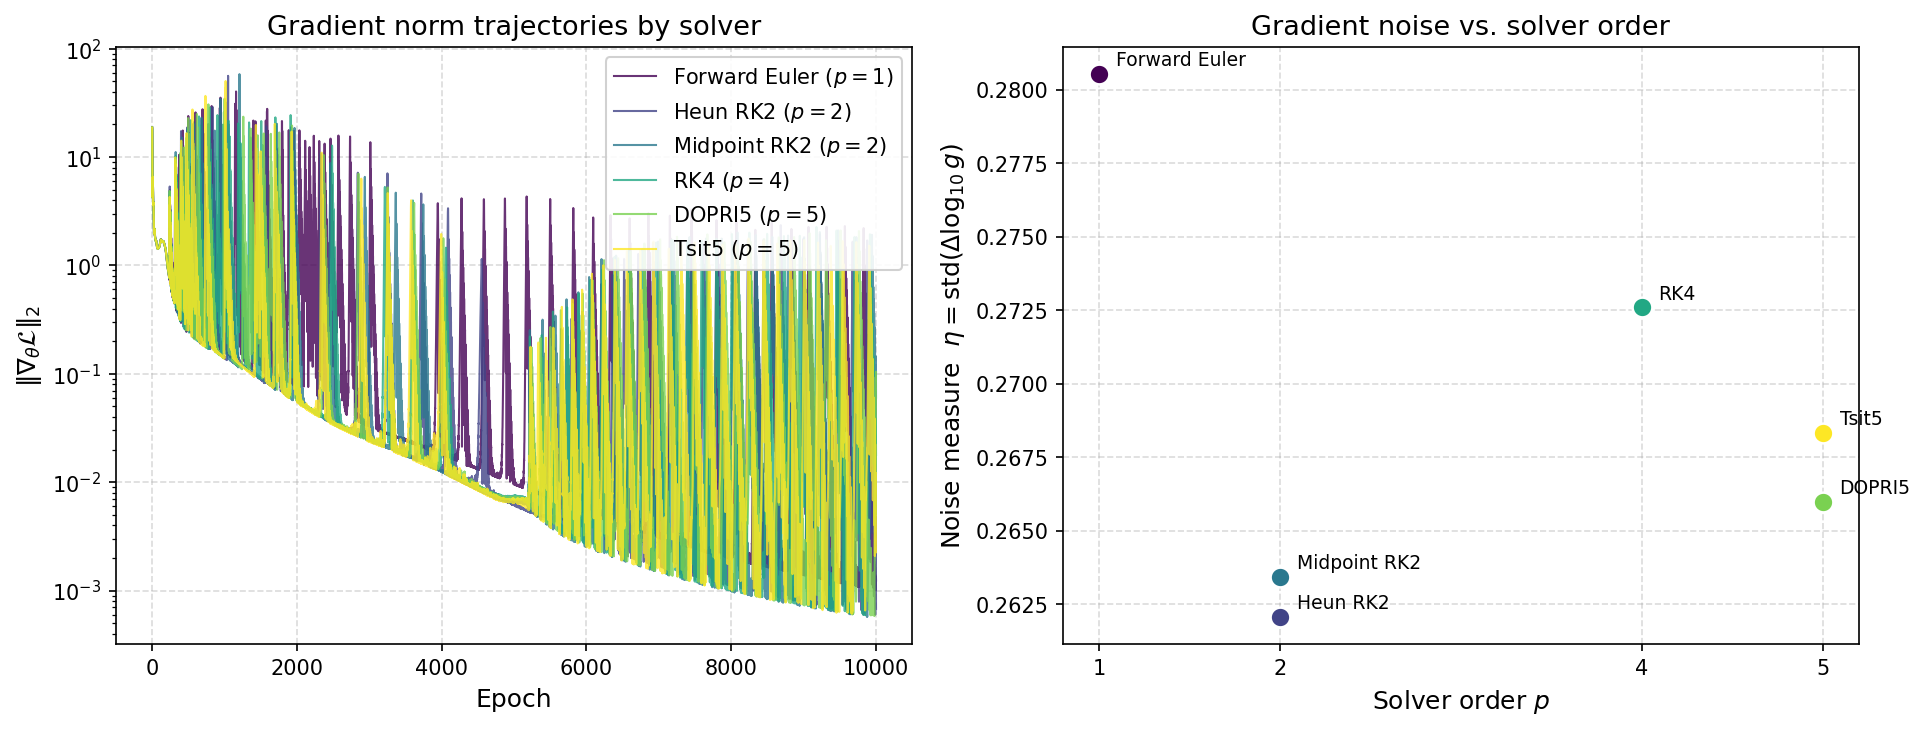
\includegraphics[width=0.8\textwidth]{figures/track_b/gradient_noise_by_order.png}
\caption{Gradient-norm traces, all six solvers: large sustained spike bursts
(one to two orders of magnitude above the local median) dominate every trace,
including Tsit5, independent of solver order.}
\label{fig:gradient-noise}
\end{figure*}

\paragraph{Finding.} Gradient-norm roughness does not explain Euler's
convergence floor. All six traces are instead dominated by shared,
order-independent spike bursts (1176 spike-epochs for Euler, 866 for Tsit5 in
the last 4000 epochs, near-identical burst structure). Four checks rule out a
numerical defect: zero non-finite gradients or losses across 60{,}000 logged
epochs; loss decreases monotonically in its running minimum for every solver;
loss is lower five epochs after a spike in $64.5\%$ of cases; and median loss
\emph{is} elevated on spike epochs ($3.90\times10^{-4}$ vs.\ $1.80\times10^{-4}$
on calm epochs), ruling out a spurious-gradient/still-loss signature. The
most plausible reading is edge-of-stability optimizer behaviour. Gradient
descent with a fixed step size and no learning-rate schedule is known to
settle into a regime where it repeatedly overshoots the walls of a narrowing
loss valley as training approaches a sharp minimum. The result is exactly
this pattern: a large transient spike followed by fast recovery, rather than
either smooth convergence or a genuine divergence. Because this behavior
appears with near-identical structure in Euler's and Tsit5's traces alike,
it is a property of the optimizer and the loss surface's local geometry, not
of the integrator's truncation error. Euler's convergence floor is better
explained by the earlier systematic-bias hypothesis
(Section~\ref{sec:solver-results}): a first-order integrator's $O(\Delta t)$
local error biases \emph{where} the optimizer settles, without making the
path it takes to get there measurably rougher.

\subsection{Learnable hybrid basis}
\label{sec:track-c}

The basis ablation (Section~\ref{sec:basis-results}) found B-spline (compact
local support, $3.9\times$ RBF's cost) and RBF (smooth global support, cheap)
statistically tied on accuracy. We therefore train the hybrid edge of
Section~\ref{sec:hybrid-method} (Equation~\ref{eq:hybrid-basis}) on
Lotka-Volterra and on the fixed pendulum (Section~\ref{sec:crossdomain}). If
one global blend systematically beat both pure bases, the basis choice in
Equation~\ref{eq:kan-edge} would be worth learning rather than fixing by
hand.

\begin{expectbox}
\expectrow{Question}{Can a network do better by learning its own blend of B-spline and RBF, rather than committing to one basis in advance?}
\expectrow{Expected}{A learned blend should match or beat the better pure basis, by adaptively favoring local support where useful and global support elsewhere.}
\expectrow{Observed}{Hybrid never beats the better pure basis on either system. On the pendulum, it actively overfits past 3000 epochs in a way pure RBF does not.}
\end{expectbox}

\begin{table*}[t]
\centering
\small
\renewcommand{\arraystretch}{1.15}
\caption{Hybrid basis vs.\ pure bases, full 10{,}000-epoch budget.}
\label{tab:hybrid-basis}
\begin{tabularx}{\textwidth}{@{}L{5.0cm} C{2.6cm} C{2.8cm} C{2.0cm} X@{}}
\toprule
\hdrrow \thh{System / basis} & \thh{Training MSE} & \thh{Extrapolation MSE} & \thh{$R^2$} & \thh{Final gate}\\
\midrule
Lotka-Volterra -- RBF (pure) & $8.83\times10^{-5}$ & $8.92\times10^{-5}$ & $1.0000$ & --\\
Lotka-Volterra -- B-spline (pure) & $7.20\times10^{-5}$ & $8.38\times10^{-5}$ & $1.0000$ & --\\
Lotka-Volterra -- Hybrid & $1.47\times10^{-4}$ & $1.78\times10^{-4}$ & $0.9999$ & $\alpha{=}0.12,\beta{=}0.88$\\
\addlinespace[2pt]
Pendulum -- RBF (pure) & $9.28\times10^{-5}$ & $0.090$ & $+0.647$ & --\\
Pendulum -- Hybrid (10,000 epochs) & $9.44\times10^{-5}$ & $\mathbf{0.809}$ & $\mathbf{-2.17}$ & $\alpha{=}0.02,\beta{=}0.98$\\
\bottomrule
\end{tabularx}
\end{table*}

\begin{figure}[tb]
\centering
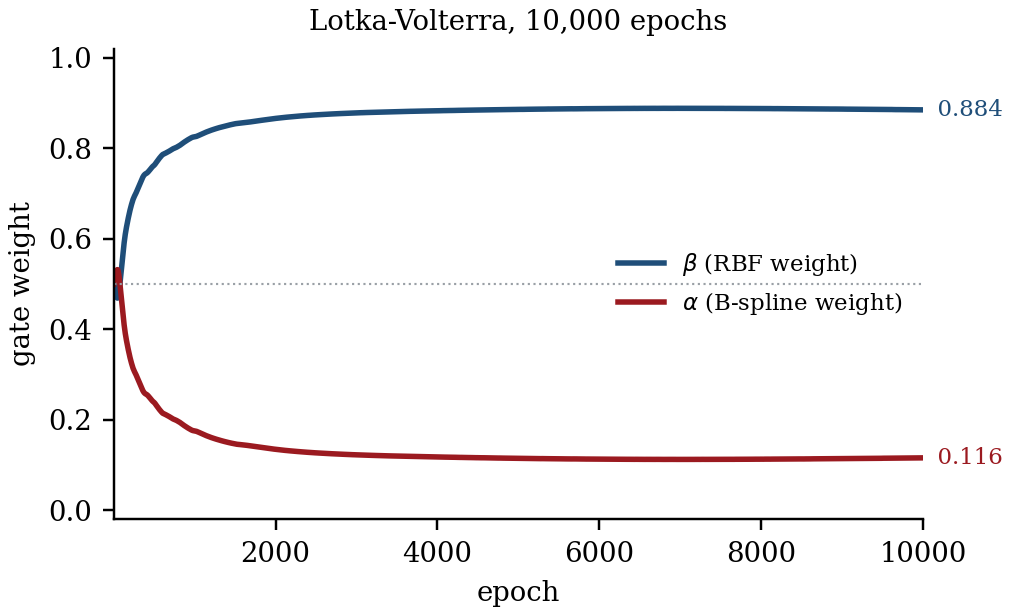
\includegraphics[width=\columnwidth]{figures/track_c/lv_full_alpha_beta.png}\\[4pt]
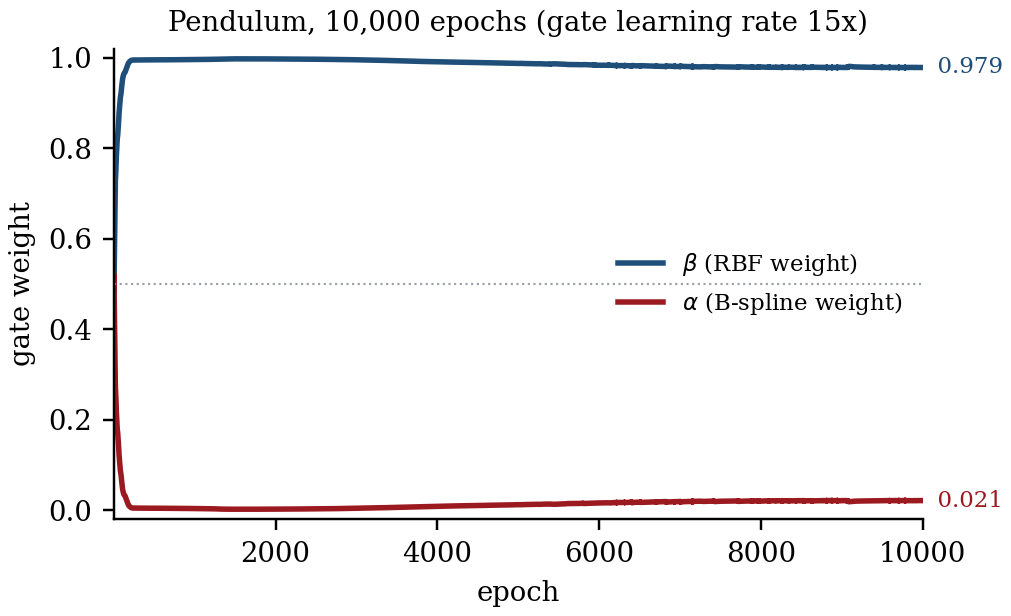
\includegraphics[width=\columnwidth]{figures/track_c/pendulum_full_alpha_beta.png}
\caption{Learned $\alpha$/$\beta$ gate evolution: Lotka-Volterra settles into a
genuine partial blend (top); the pendulum gate reaches $\approx\!99.5\%$
RBF by epoch 250 and ends at $98\%$ (bottom); it settles well before the
overfitting onset discussed below.}
\label{fig:hybrid-gates}
\end{figure}

\paragraph{Lotka-Volterra: no benefit, real cost.} The gate settles into a
genuine partial blend, retaining $\approx\!12\%$ B-spline, which confirms the
mechanism works as designed. Hybrid ties both pure bases on final accuracy
while paying roughly the \emph{sum} of their per-epoch compute.

\paragraph{Pendulum: overfitting emerges only past a specific budget.} A
short probe run at 2000 epochs first surfaced a practical wrinkle. The gate
moved in the correct direction (toward RBF) but too slowly, so the network
still carried meaningful B-spline contamination at an epoch count where the
pure-RBF pendulum recipe was already nearly converged. Giving the gate its
own, faster learning rate ($15\times$ the base rate, direction untouched)
closed nearly all of that gap at the same probe budget
(Figure~\ref{fig:hybrid-probe}, top), and we carried this into the full run.

\begin{figure}[tb]
\centering
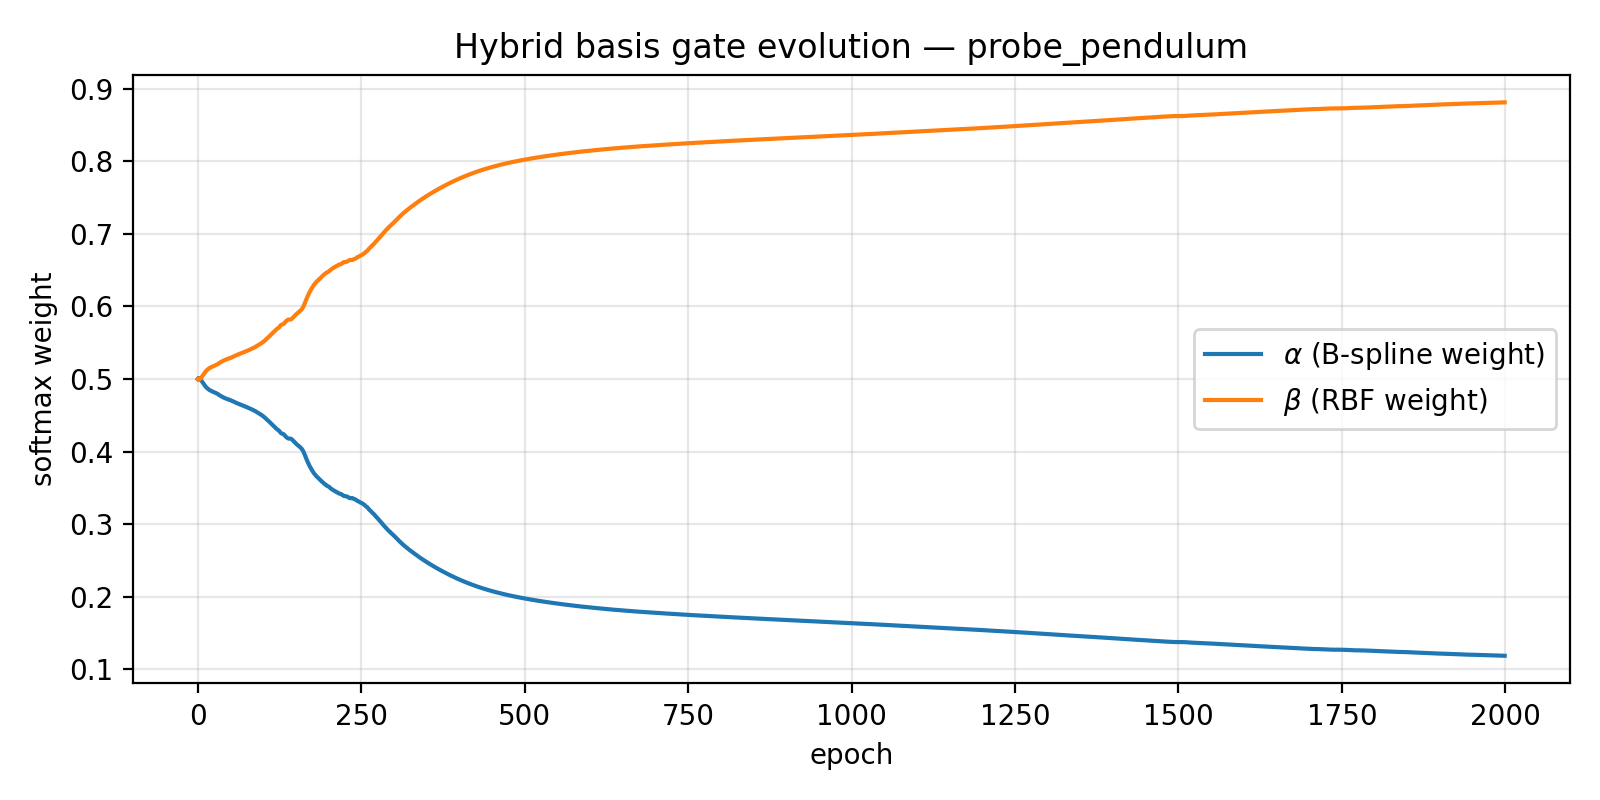
\includegraphics[width=\columnwidth]{figures/track_c/hybrid_probe_pendulum_alpha_beta.png}\\[4pt]
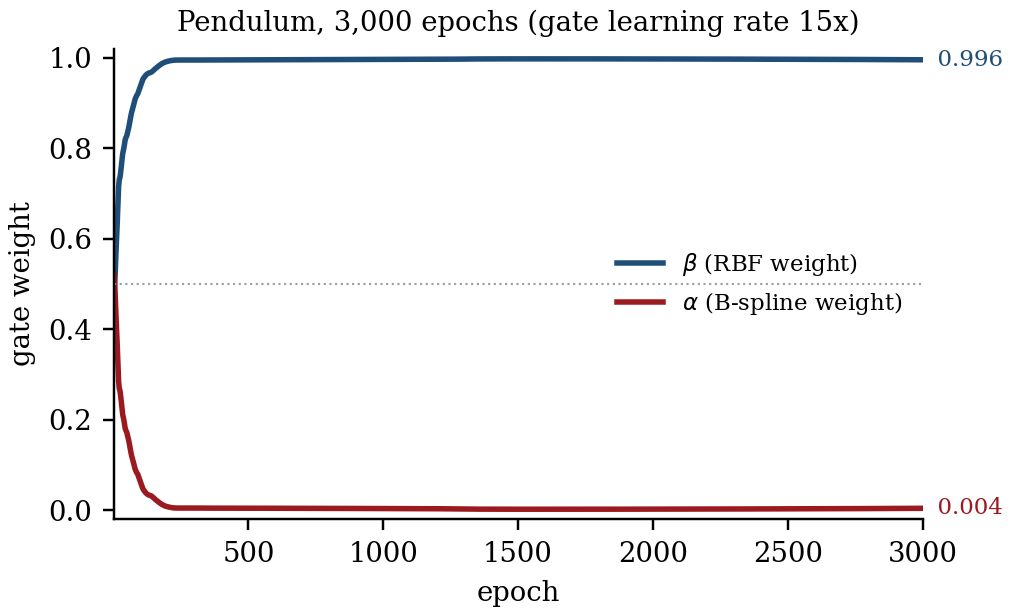
\includegraphics[width=\columnwidth]{figures/track_c/hybrid_pendulum_3k_alpha_beta.png}
\caption{Top: the 2000-epoch probe run's gate trace, showing the slow drift
toward RBF that motivated the gate-learning-rate fix. Bottom: the gate trace
for the 3000-epoch pre-overfitting-optimum run discussed below, settling to
$\beta\approx0.996$.}
\label{fig:hybrid-probe}
\end{figure}

At the full 10{,}000-epoch budget, hybrid matches pure RBF's training fit
almost exactly, but its extrapolation collapses ($R^2=-2.17$). The monitor
loss bottoms out near epoch 2950 ($\approx0.054$), then rises to a
$\approx0.4$ plateau for the remaining 7000 epochs while training loss keeps
improving. This is textbook overfitting, visible directly in the saved
training history. The gate settles well before this onset: $\beta$ reaches
$\approx0.995$ by epoch 250, some 2750 epochs before overfitting begins, and
pure RBF trained on the identical recipe shows no such pattern at all.
Capping training at the pre-overfit optimum (epoch 3000, chosen from the
10,000-epoch run's own point of minimum monitor loss) shows hybrid
\emph{ahead} of pure RBF at the same epoch count ($0.055$ vs.\ $0.081$
full-horizon MSE) with extrapolation $R^2=+0.580$, approaching pure RBF's
fully-converged number ($+0.647$). Figure~\ref{fig:hybrid-pendulum-runs} shows
both runs side by side: the loss curves of the full run make the overfitting
onset visible, and its phase portrait shows the extrapolation collapsing into
a small wrong loop, while the 3000-epoch run still follows the decaying
spiral.

\begin{figure*}[t]
\centering
\begin{minipage}[c]{0.56\textwidth}
\centering
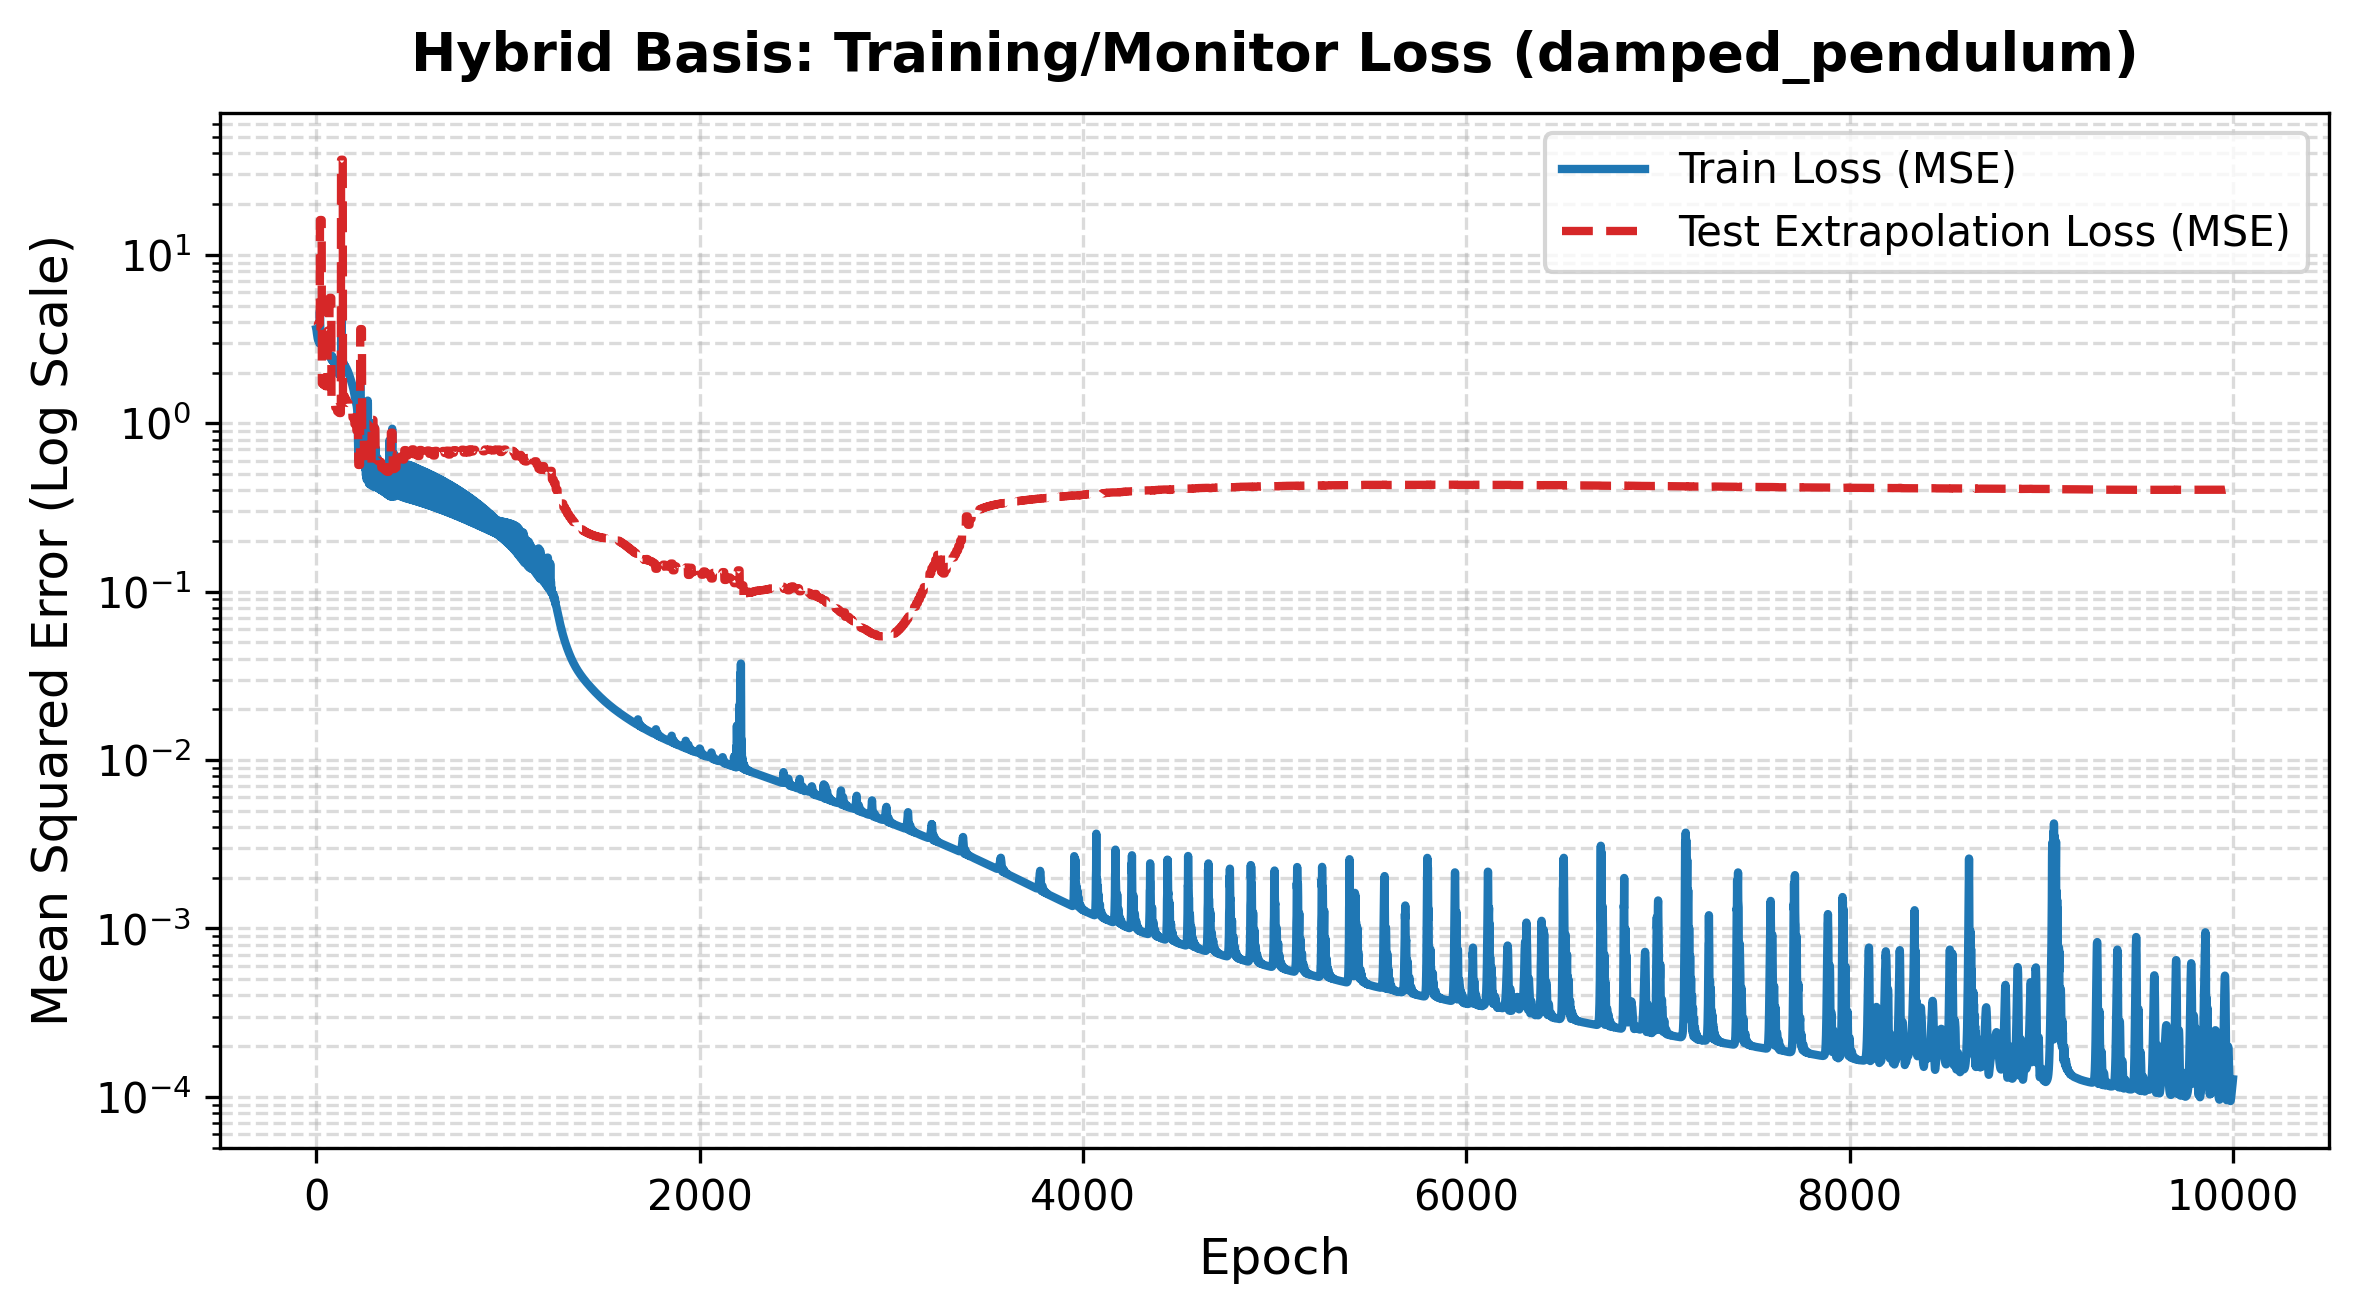
\includegraphics[width=\linewidth]{figures/track_c/pendulum_full_loss_curves.png}
\end{minipage}\hfill
\begin{minipage}[c]{0.40\textwidth}
\centering
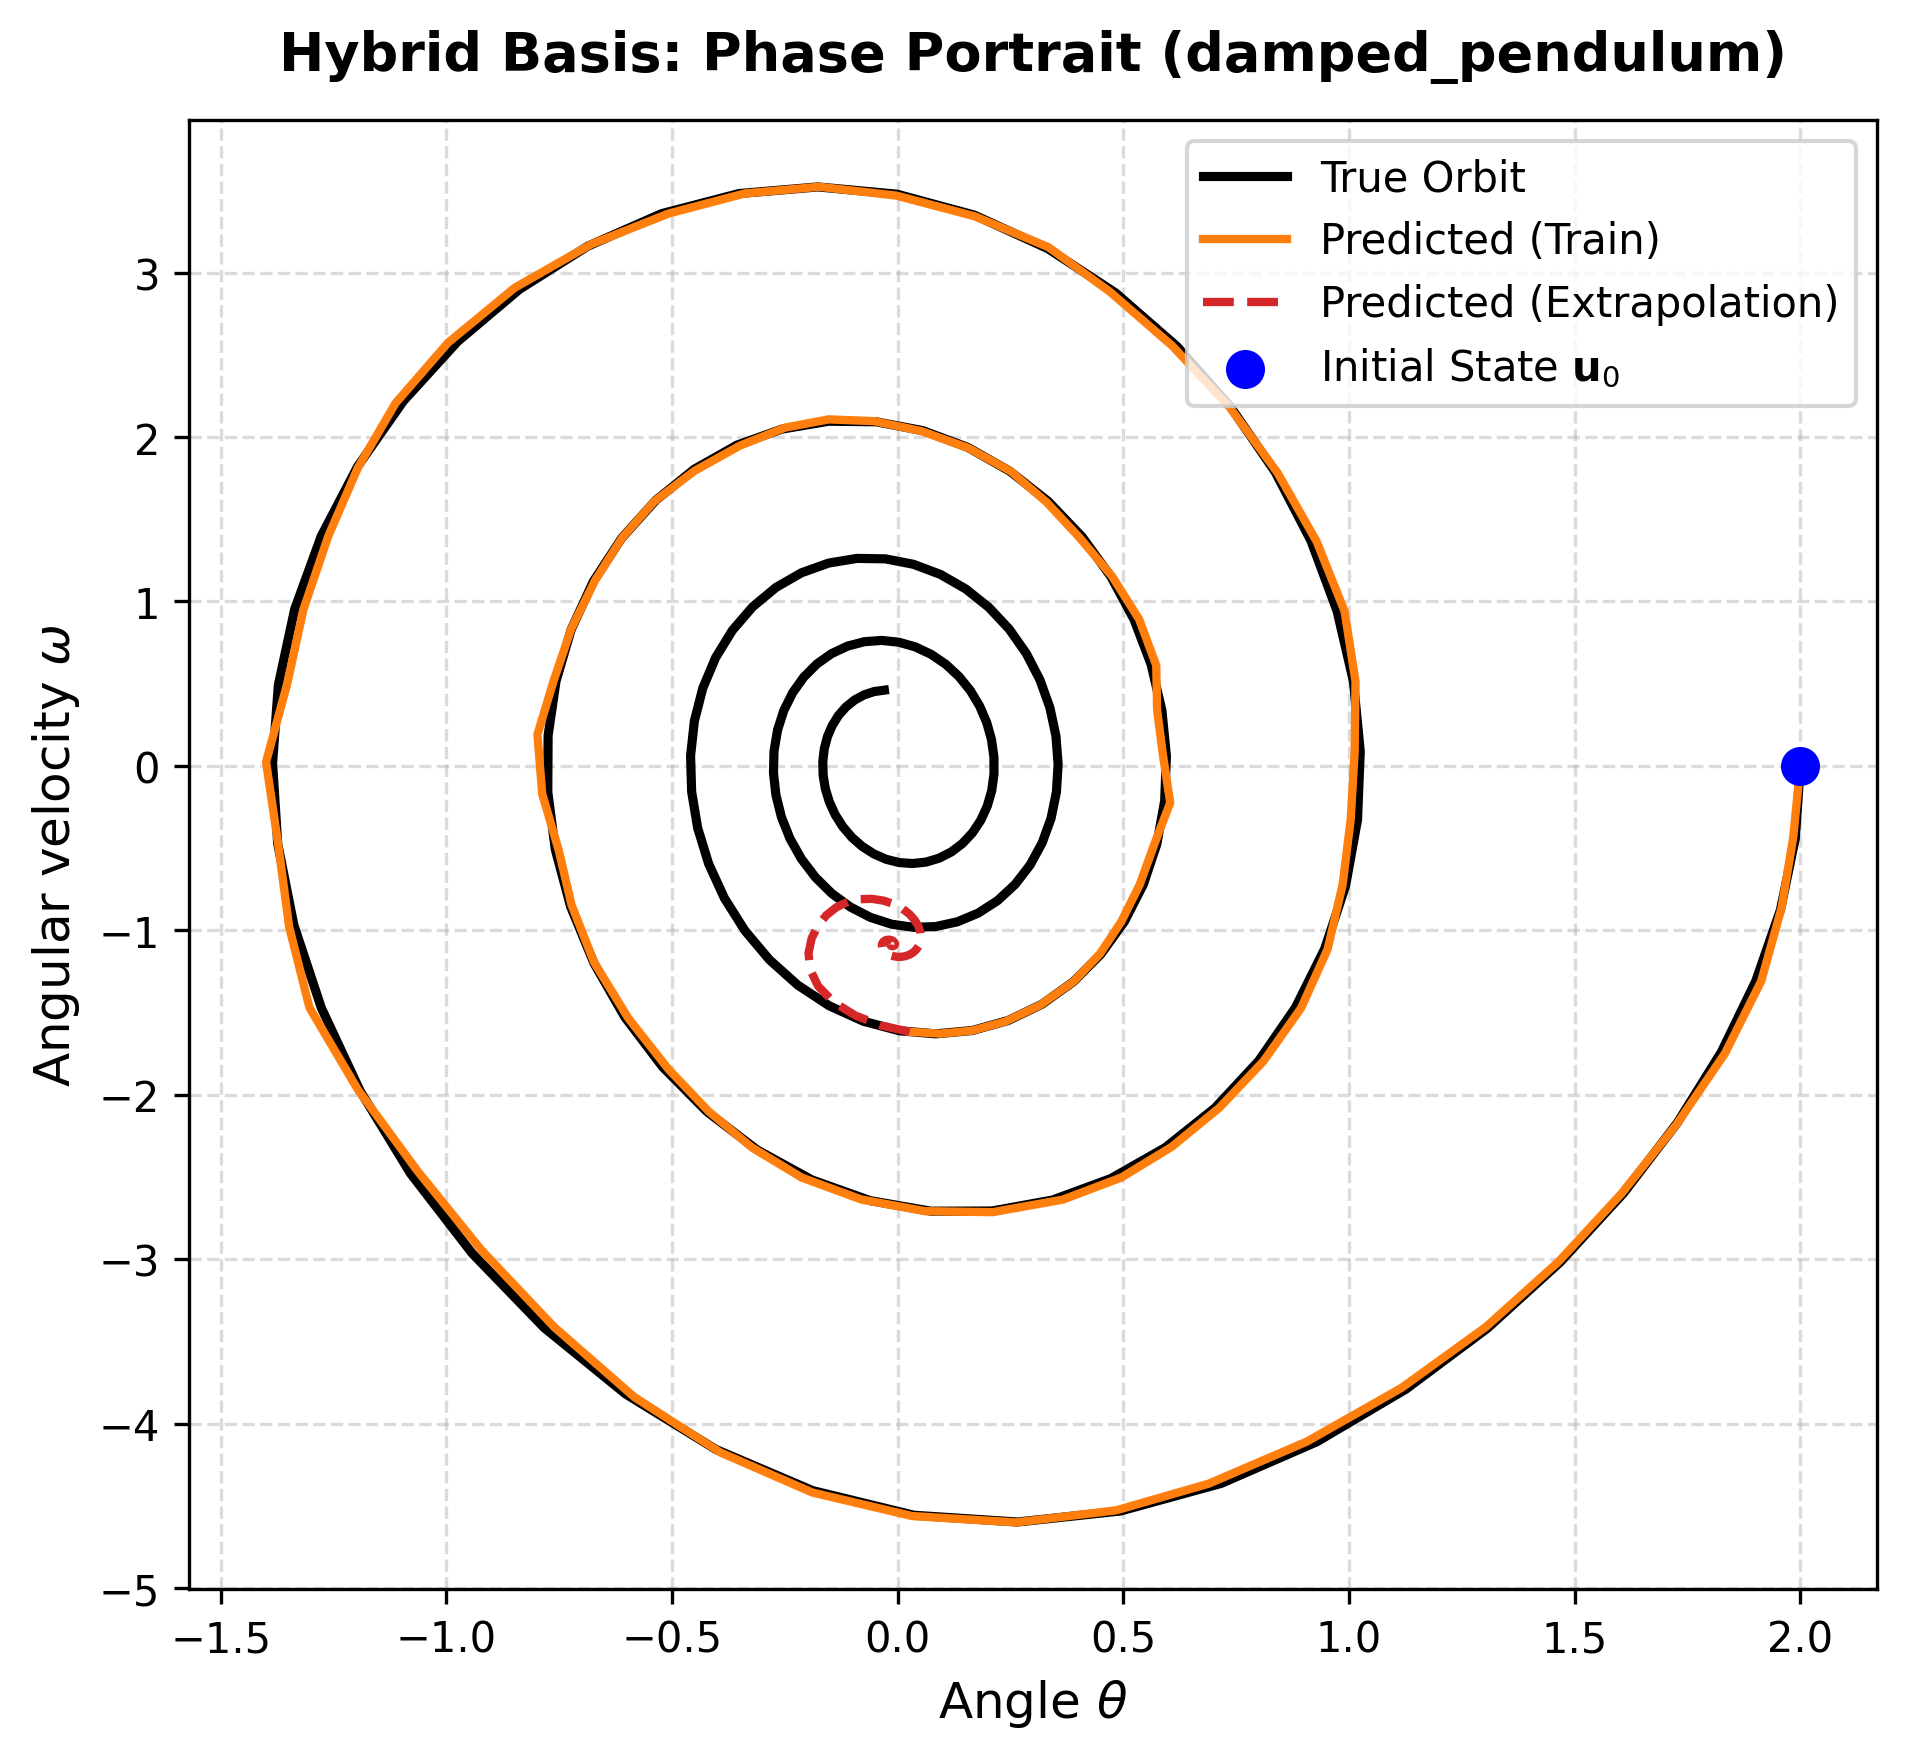
\includegraphics[width=\linewidth]{figures/track_c/pendulum_full_phase_space.png}
\end{minipage}\\[6pt]
\begin{minipage}[c]{0.56\textwidth}
\centering
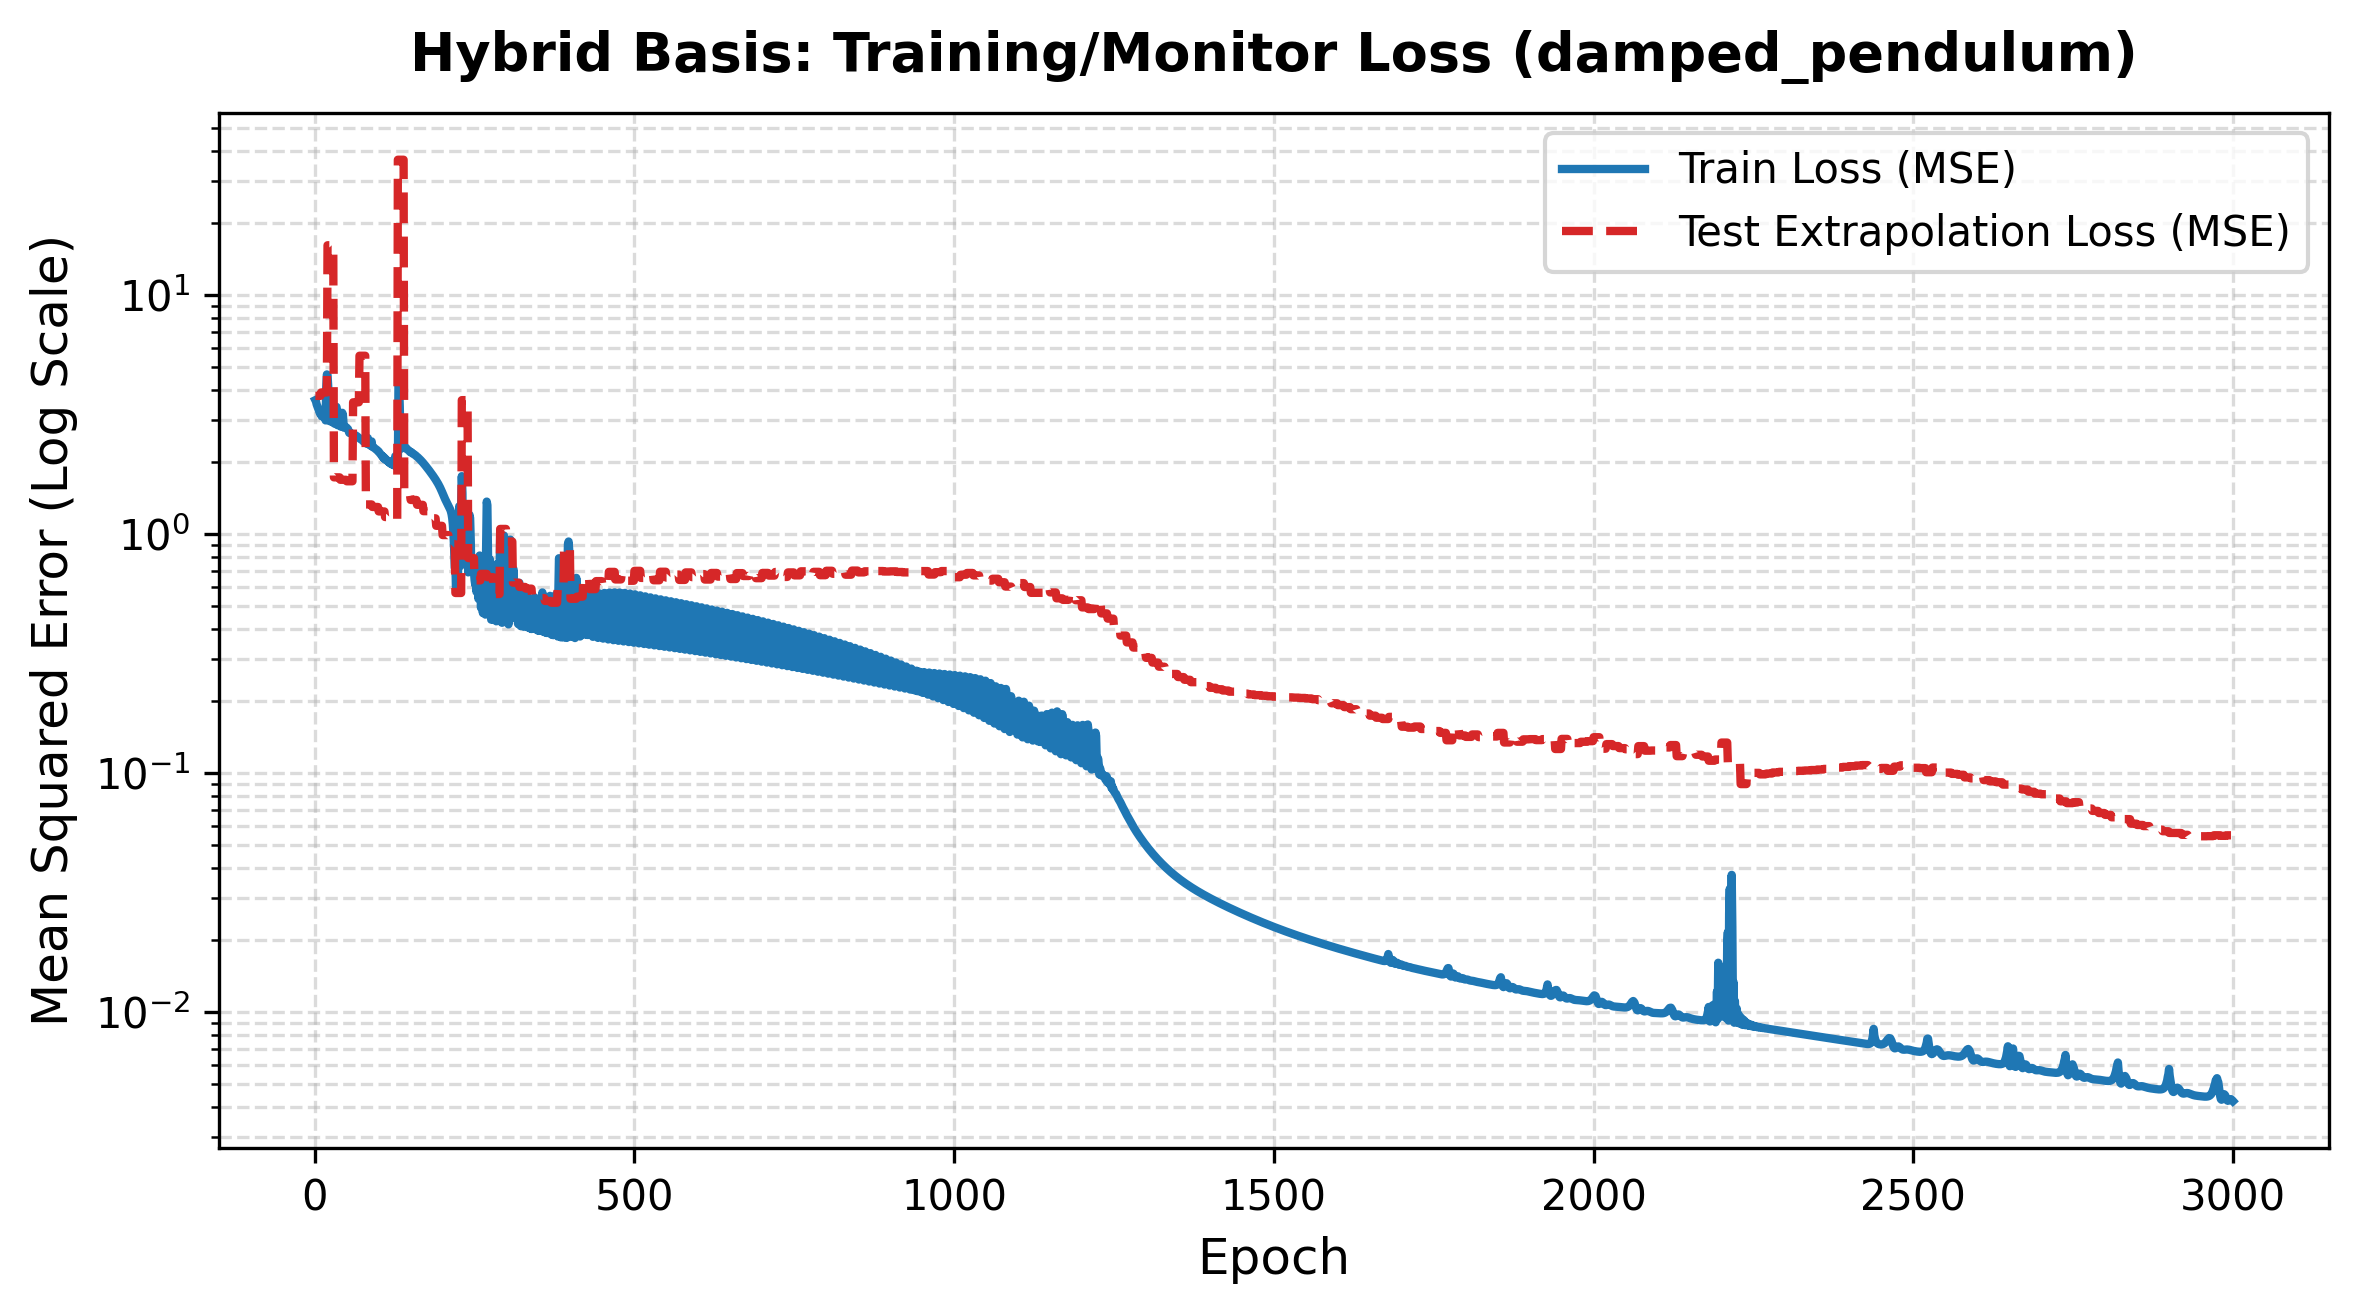
\includegraphics[width=\linewidth]{figures/track_c/pendulum_3k_loss_curves.png}
\end{minipage}\hfill
\begin{minipage}[c]{0.40\textwidth}
\centering
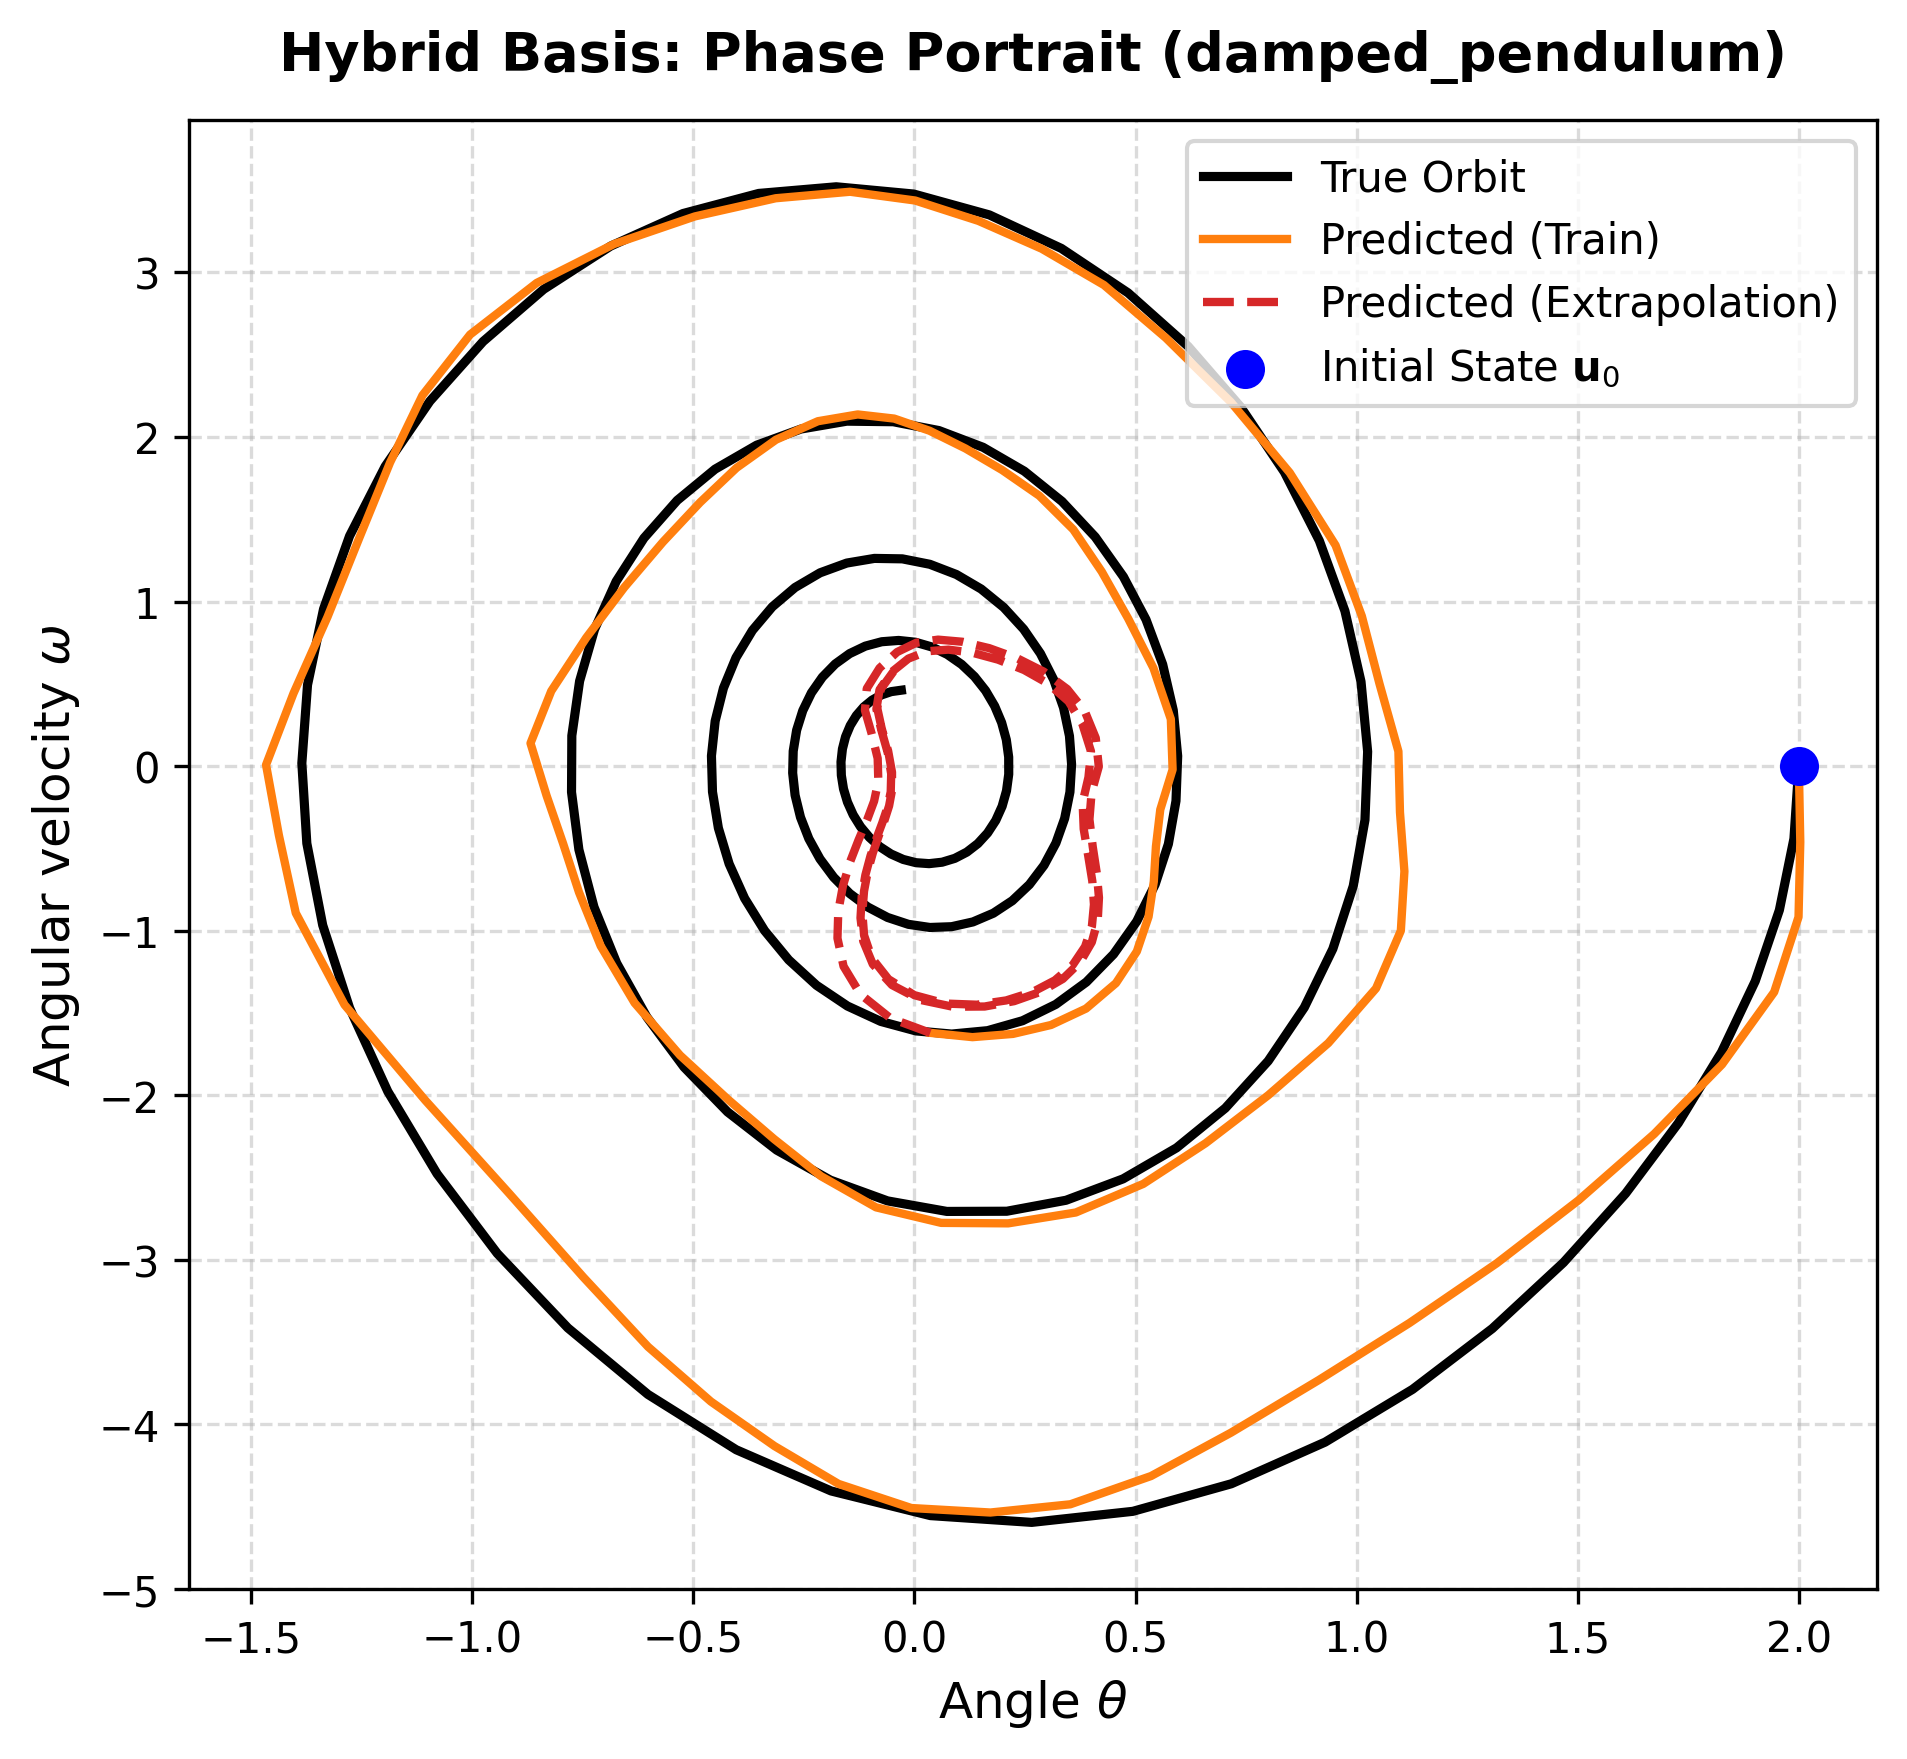
\includegraphics[width=\linewidth]{figures/track_c/pendulum_3k_phase_space.png}
\end{minipage}
\caption{Hybrid basis on the pendulum. Top: the full 10{,}000-epoch
run; training loss keeps falling while the extrapolation (monitor) loss
bottoms out near epoch 2950 and climbs back to $\approx0.4$ (left), and the
extrapolated orbit collapses into a small wrong loop (right). Bottom: the same
recipe stopped at 3000 epochs; train and monitor loss fall together (left)
and the extrapolation follows the decaying spiral (right).}
\label{fig:hybrid-pendulum-runs}
\end{figure*}

\begin{keypoint}[Verdict]
The learnable hybrid basis never outperforms the better pure basis on either
system at any budget tested. Its gate mechanism works exactly as designed
(gradient-driven, converging differently and sensibly per system), but that
alone does not buy an accuracy edge. On the pendulum specifically, a
network that \emph{starts} as a blend generalizes measurably worse over long
training than one that starts pure RBF, despite an almost-identical final
gate and matching training accuracy.
\end{keypoint}

\subsection{Stiffness--solver map and loss landscape}
\label{sec:track-d}

Numerical stiffness (a system whose fastest and slowest timescales differ by
orders of magnitude) is where explicit integrators are classically expected
to struggle. We sweep damping ratio
$\mu\in\{0.1,0.5,1.0,2.0,5.0,8.0\}$ against four explicit solvers \{Euler,
Midpoint, RK4, Tsit5\} \cite{tsitouras2011tsit5} on the damped pendulum, at a
fixed step $\Delta t=0.05$. The goal is to map which $(\text{solver},\mu)$
combinations converge and which fail, and to test whether any failure is
actually a stiffness effect.

\begin{expectbox}
\expectrow{Question}{As damping ratio increases the pendulum's dynamics stiffen -- do lower-order explicit solvers genuinely fail as stiffness grows?}
\expectrow{Expected}{Higher damping ratios should push some (solver, $\mu$) combinations outside that solver's classical stability region, producing divergence.}
\expectrow{Observed}{Linear stability theory predicts zero divergences at every tested $\mu$, and the sweep confirms it. Every observed failure traces to random seed, not stiffness.}
\end{expectbox}

\subsubsection{The stability question resolves quickly}

Linearizing at equilibrium gives eigenvalues
$\lambda = \big({-\mu\pm\sqrt{\mu^2-4g/L}}\big)/2$. For every underdamped
$\mu<2\sqrt{g/L}\approx6.26$, $|\lambda|=\sqrt{g/L}\approx3.13$ is constant, so
$h|\lambda|\approx0.157$ at $\Delta t=0.05$, far inside even Euler's
stability region $h|\lambda|\le2$ \cite{dahlquist1963stability}. Even the
overdamped case ($\mu=8.0$, fast eigenvalue $\lambda_{\text{fast}}\approx-7.7$)
gives $h|\lambda_{\text{fast}}|\approx0.385$, still comfortably stable. This
predicts, and the sweep confirms, zero divergences across all 24 cells: not
one run produced an invalid gradient at any point in training. All four
solvers tested are explicit Runge-Kutta methods with a bounded stability
region. We implement no implicit solver, so this analysis cannot say whether
an implicit method would behave differently at a genuinely stiffer
configuration.

\subsubsection{What actually drives the failures: initialization}

\begin{table*}[t]
\centering
\footnotesize
\renewcommand{\arraystretch}{1.15}
\caption{Original 24-cell sweep (single seed 42), best training MSE and verdict.}
\label{tab:stiffness-single-seed}
\begin{tabularx}{\textwidth}{@{}C{1.6cm} X X X X@{}}
\toprule
\hdrrow \thh{Damping ratio $\mu$} & \thh{Euler} & \thh{Midpoint} & \thh{RK4} & \thh{Tsit5}\\
\midrule
0.1 & unstable, $1.7\times10^{-2}$ & unstable, $3.0\times10^{-2}$ & unstable, $2.2\times10^{-2}$ & unstable, $2.4\times10^{-2}$\\
0.5 & \textbf{converged}, $4.6\times10^{-3}$ & \textbf{converged}, $7.9\times10^{-3}$ & \textbf{converged}, $4.7\times10^{-3}$ & \textbf{converged}, $9.2\times10^{-3}$\\
1.0 & unstable, $1.0\times10^{-1}$ & converged, $5.4\times10^{-4}$ & converged, $5.3\times10^{-4}$ & converged, $4.0\times10^{-4}$\\
2.0 & unstable, $1.8\times10^{-2}$ & unstable, $1.8\times10^{-2}$ & unstable, $1.8\times10^{-2}$ & unstable, $1.8\times10^{-2}$\\
5.0 & converged, $6.1\times10^{-5}$ & converged, $7.0\times10^{-5}$ & converged, $6.9\times10^{-5}$ & converged, $6.8\times10^{-5}$\\
8.0 & converged, $2.1\times10^{-5}$ & converged, $2.3\times10^{-5}$ & converged, $2.6\times10^{-5}$ & converged, $2.6\times10^{-5}$\\
\bottomrule
\end{tabularx}
\end{table*}

\begin{figure}[tb]
\centering
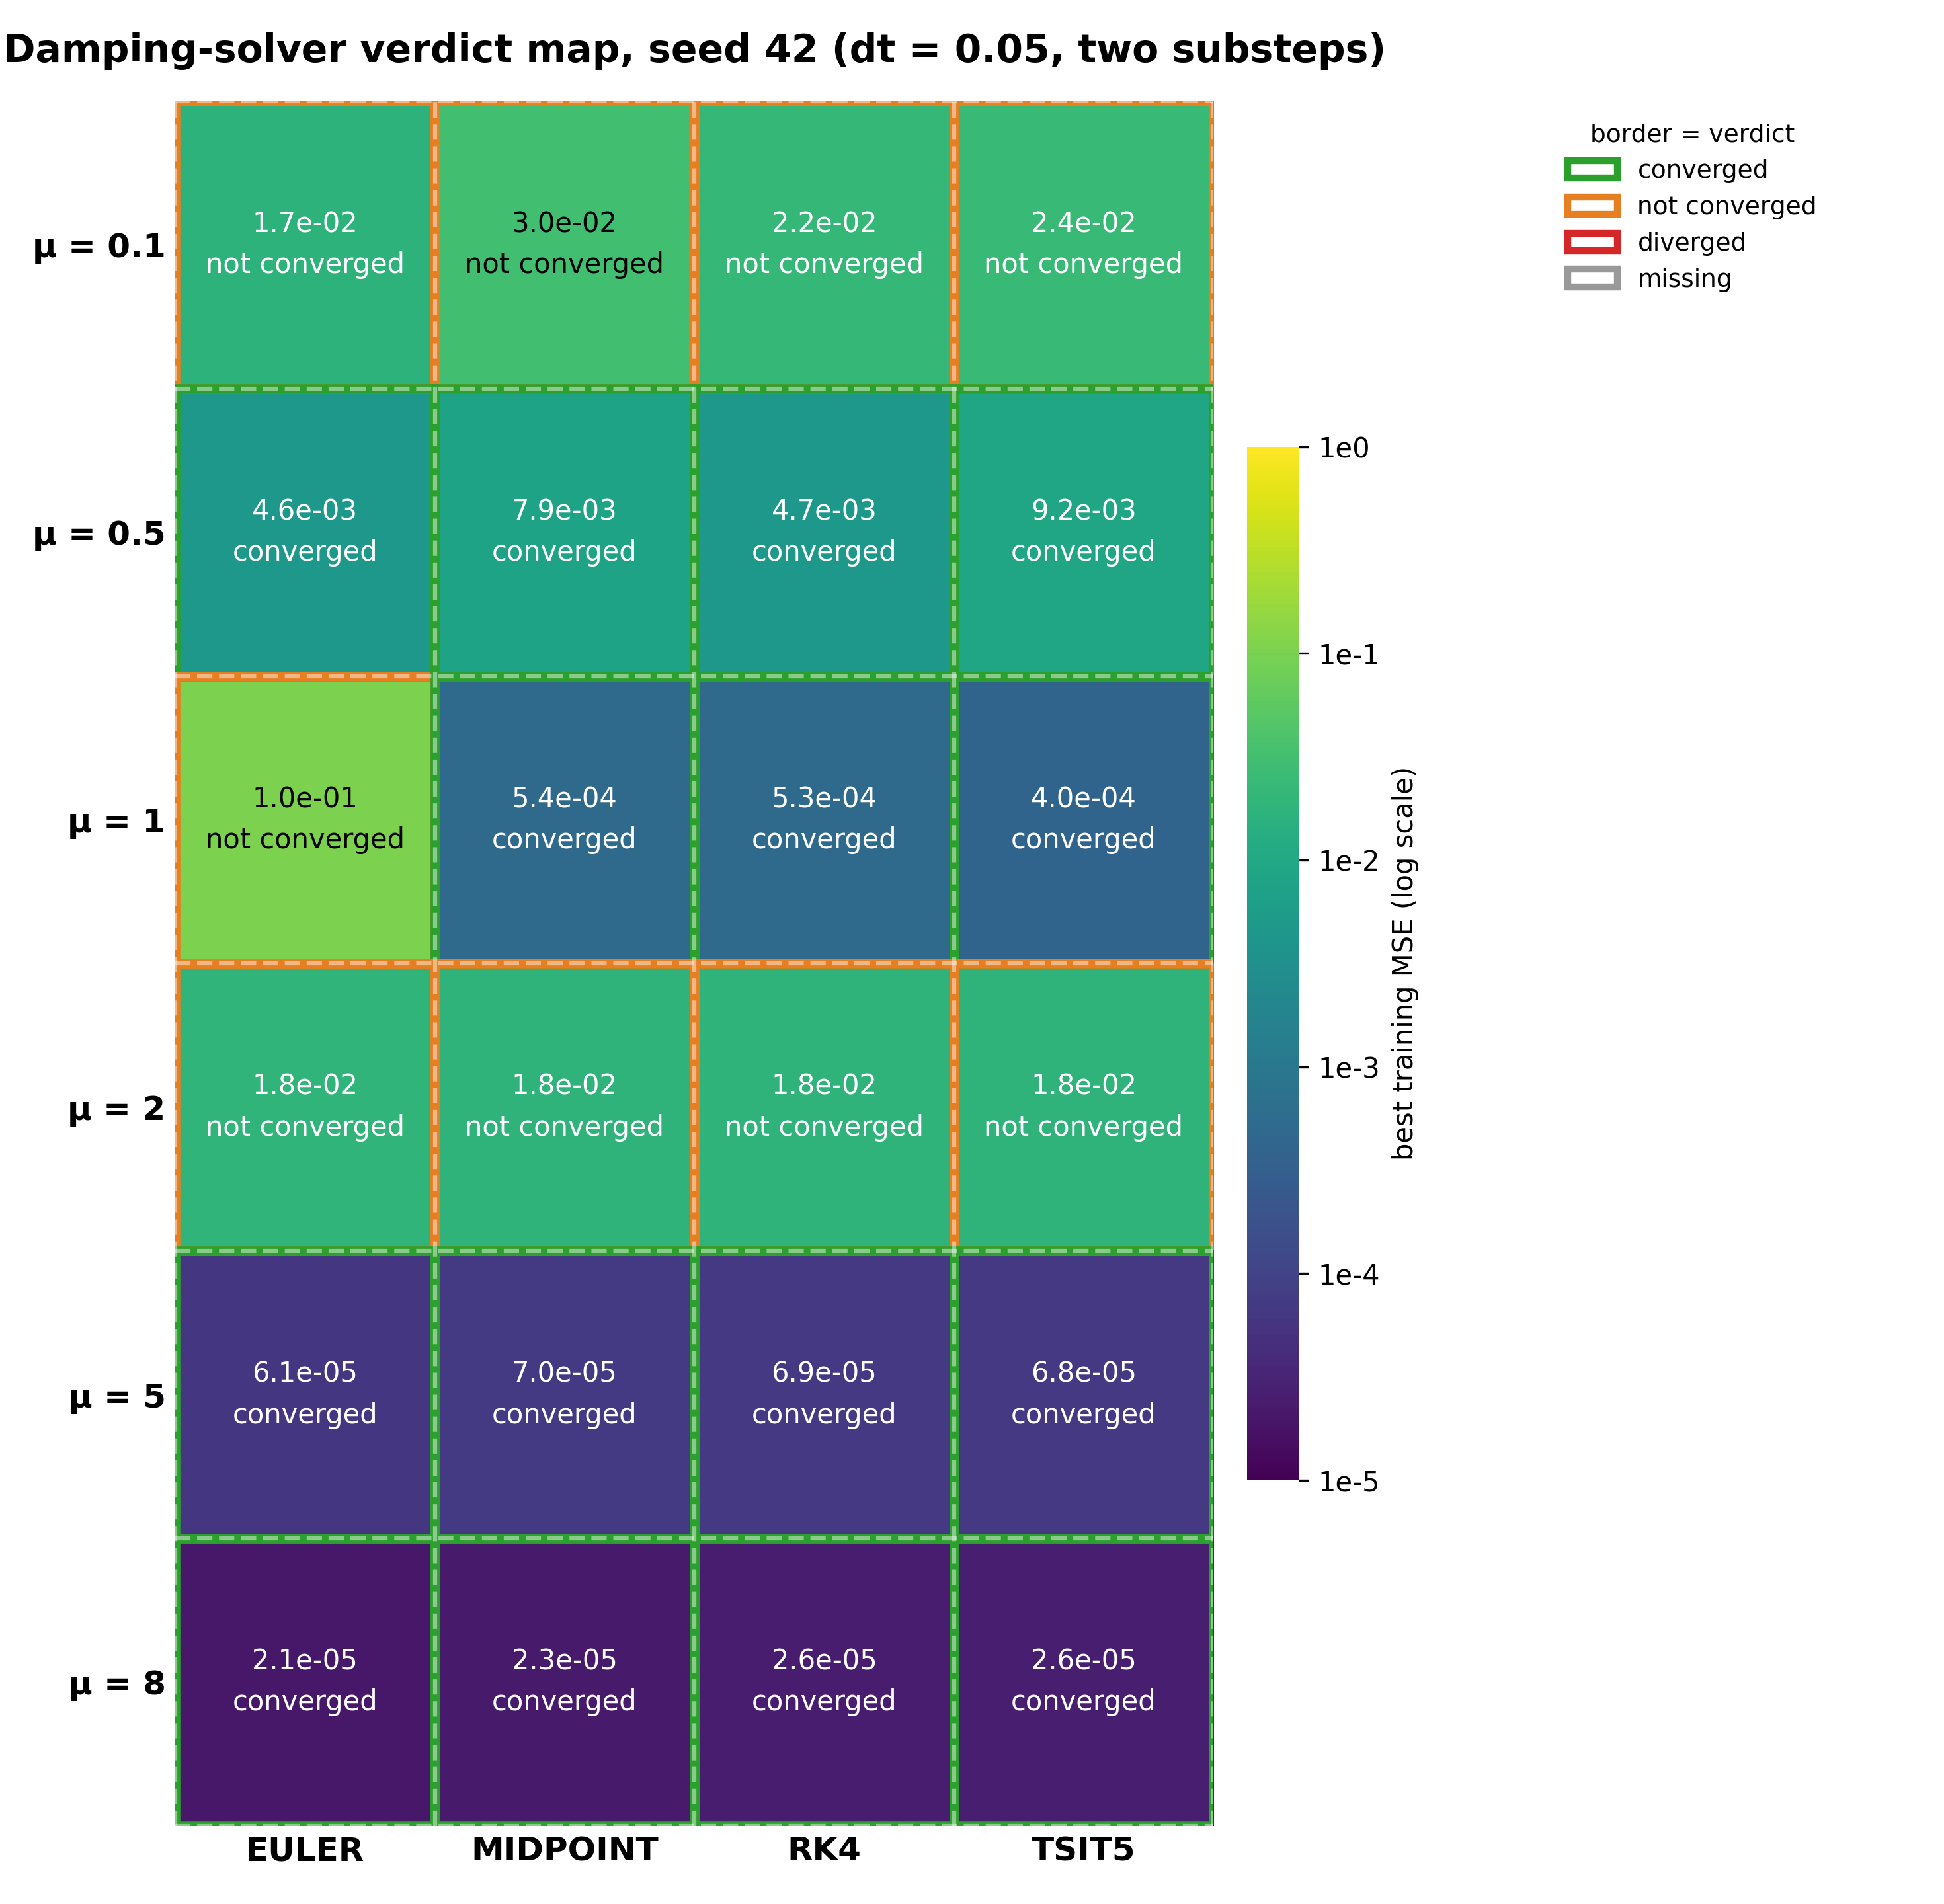
\includegraphics[width=0.85\columnwidth]{figures/track_d/stability_heatmap_dt0.05.png}
\caption{Stability verdict heatmap, 24-cell single-seed probe sweep, $\Delta t=0.05$.}
\label{fig:stability-heatmap}
\end{figure}

Two anomalies stand out: $\mu=2.0$ fails identically across all four solvers
to two significant figures, and $\mu=1.0$ fails only for Euler. Retraining
Euler at $\mu=2.0$ with two more seeds isolates the cause (seed 42: unstable,
$1.82\times10^{-2}$; seed 1: unstable, $1.68\times10^{-2}$; seed 7:
\textbf{converged}, $7.09\times10^{-5}$): the trap depends on the random
initialization. Extending this to all four solvers $\times$ six $\mu$
$\times$ three seeds (72 cells, checkpoints saved throughout) confirms the
pattern generally. Only the two extremes ($\mu=0.1$, uniformly hard;
$\mu\in\{5.0,8.0\}$, uniformly easy) hold their verdict across every seed.
Every transitional $\mu\in\{0.5,1.0,2.0\}$ has at least one of three seeds
land in a bad local minimum. At $\mu=1.0$, two \emph{different} seeds fail
for two different reasons: seed 1 produces a universally bad initialization
shared by all four solvers (MSE $\approx9.7\text{--}9.8\times10^{-2}$, the
same signature as the $\mu=2.0$ shared trap), while seed 42 carries a second,
Euler-specific failure on top of it. Euler's apparent $\mu=1.0$ weakness in
Table~\ref{tab:stiffness-single-seed} is therefore the sum of two separate
effects, one shared and one solver-specific, compressed into a single
misleading number.

\begin{keypoint}[Consequence for the original heatmap]
The 24-cell sweep used one shared seed for all four solvers. All four solvers
failing identically at $\mu=2.0$ reflects four solvers inheriting the same
coin flip from a shared initialization, at this step size the seed$\times\mu$
interaction determines outcome far more than solver choice does.
\end{keypoint}

\subsubsection{The mechanism: a genuine spurious equilibrium}

We evaluated a checkpoint saved for Euler's trapped $\mu=2.0$ run at the true
equilibrium and at a nearby grid-search minimum. The learned field
$f_\theta$ has a large nonzero derivative at $(0,0)$ ($|f_\theta|=2.74$) and a
genuine, stable, spurious equilibrium $0.05$--$0.07$ units away
($|f_\theta|=0.0086$). This holds independently for all four solvers' own
trained models ($|f_\theta(0,0)|\in[2.65,2.88]$ across euler, midpoint, rk4,
tsit5): all four independently-trained networks converge to essentially the
same wrong fixed point.

\begin{figure*}[t]
\centering
\begin{minipage}[t]{0.37\textwidth}
\centering
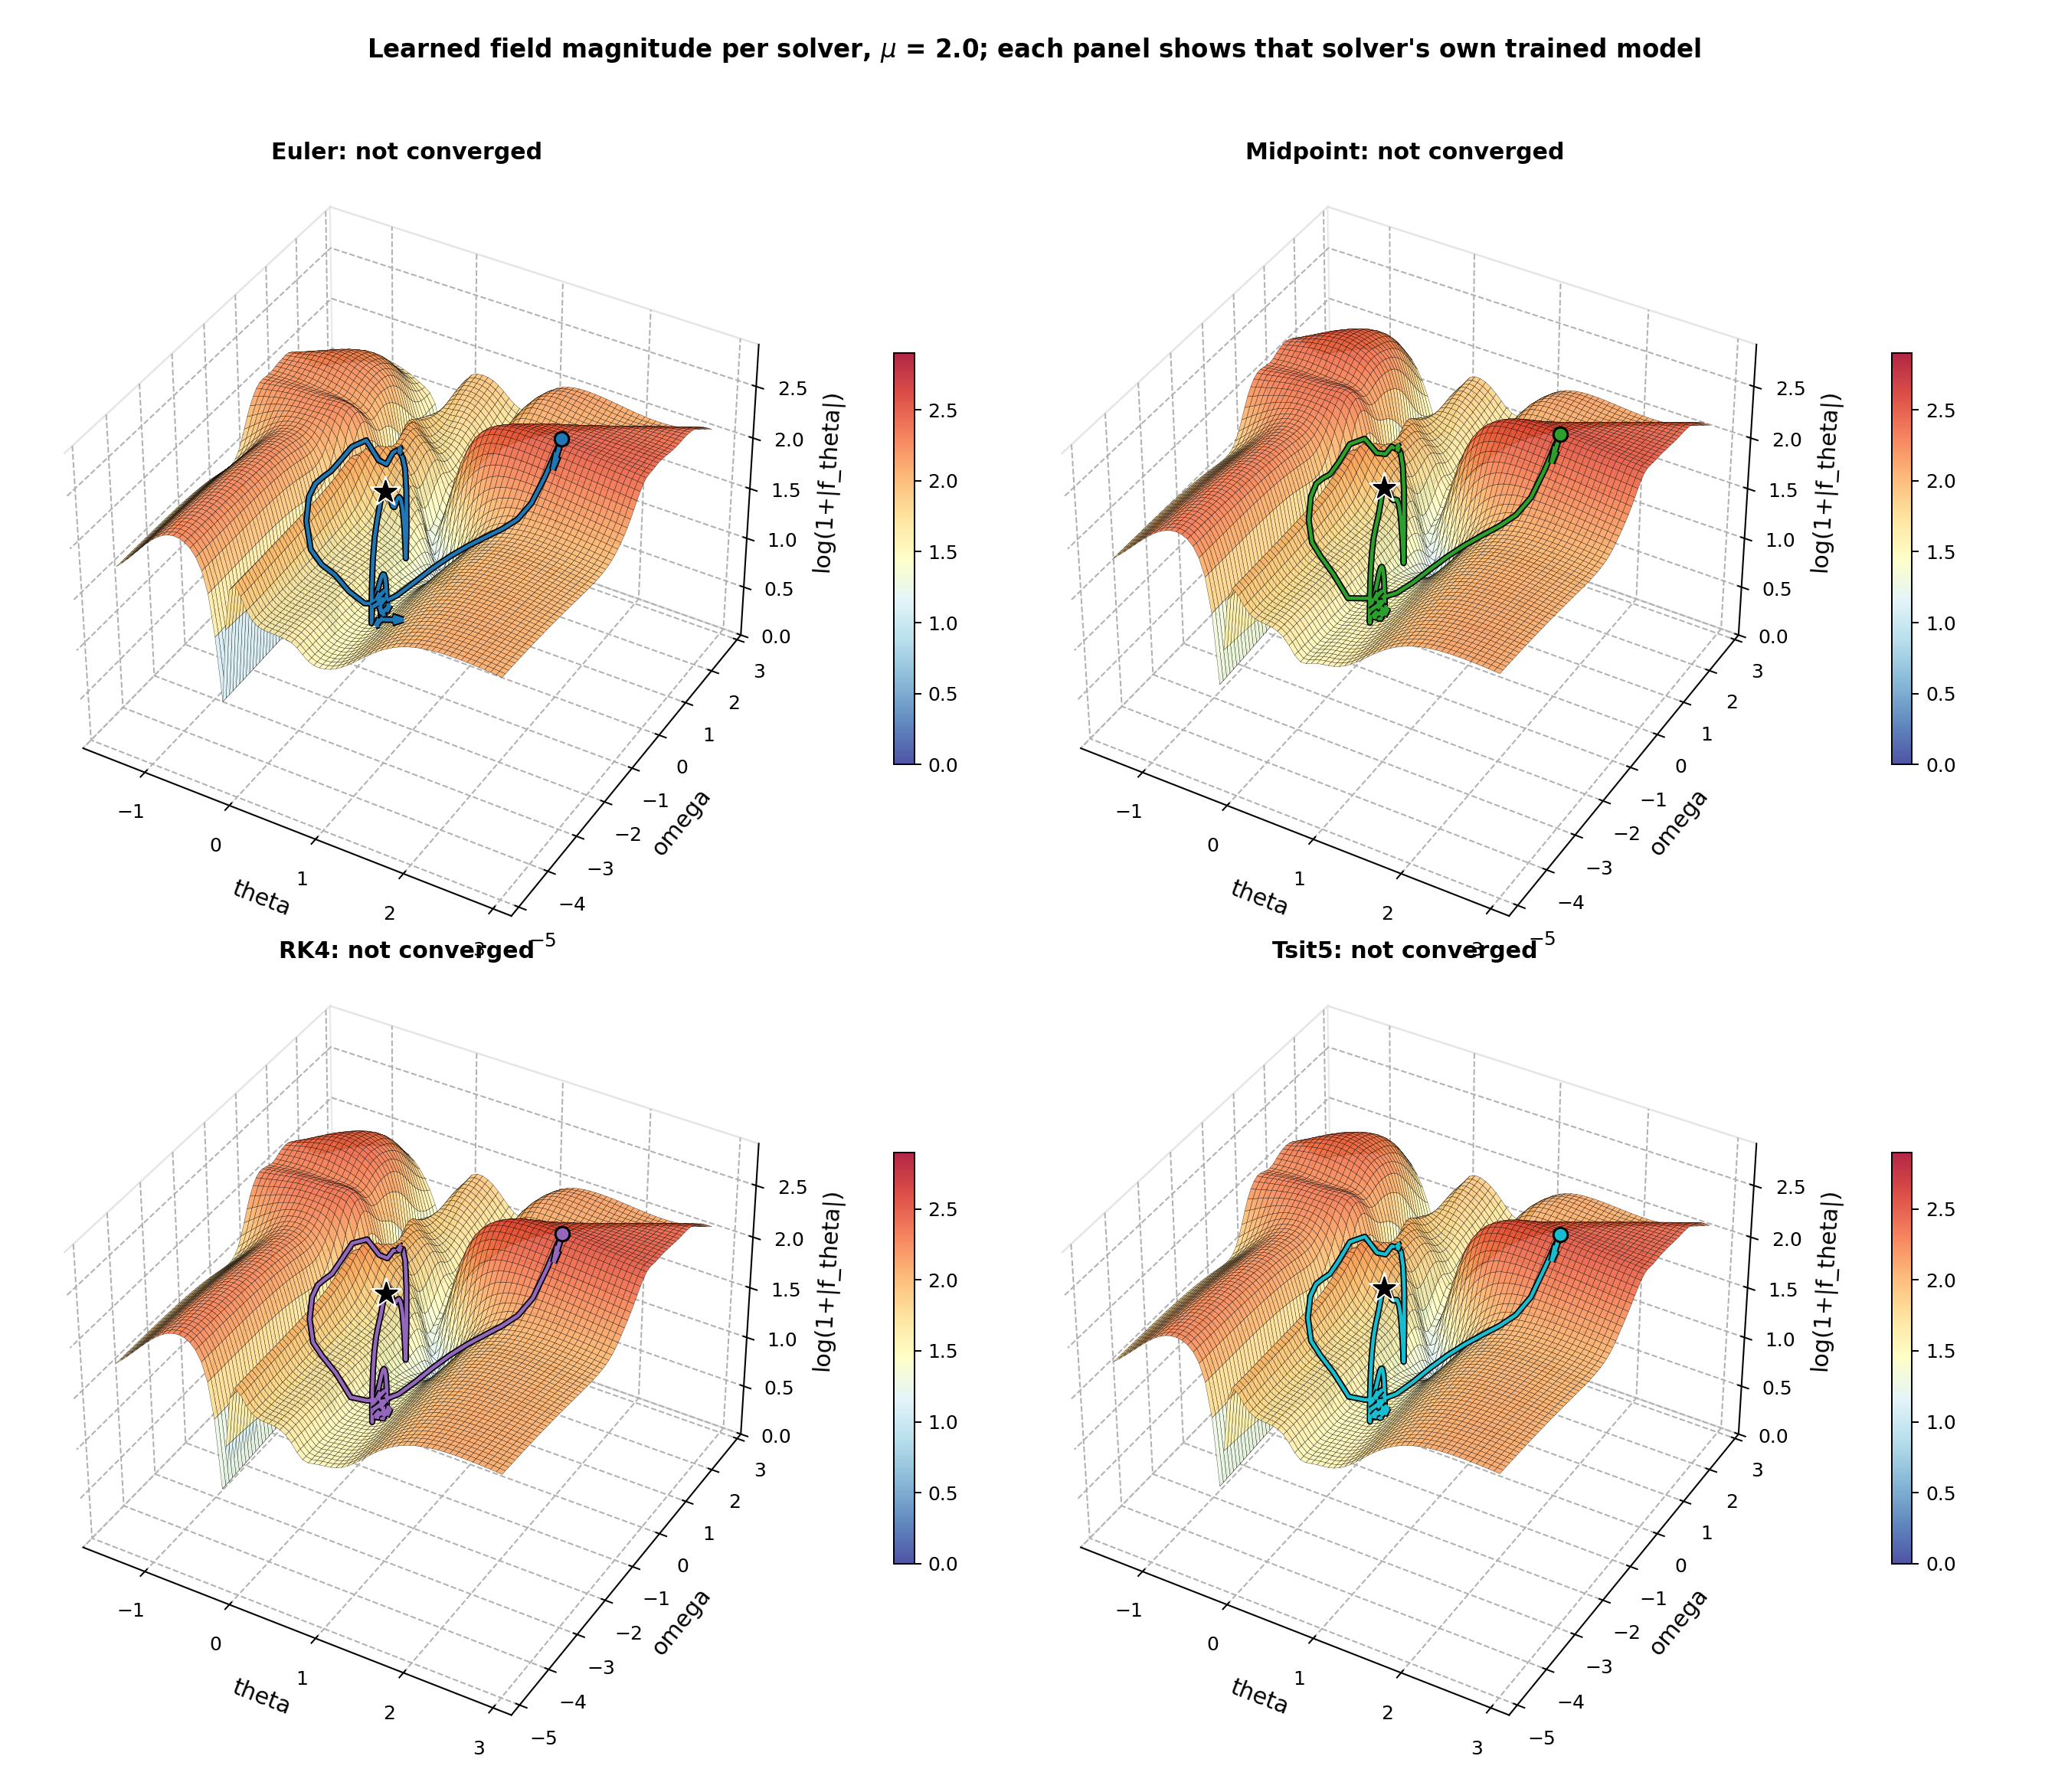
\includegraphics[width=\linewidth]{figures/track_d/phase_portrait_3d_mu2.0.png}
\end{minipage}\hspace{0.04\textwidth}
\begin{minipage}[t]{0.37\textwidth}
\centering
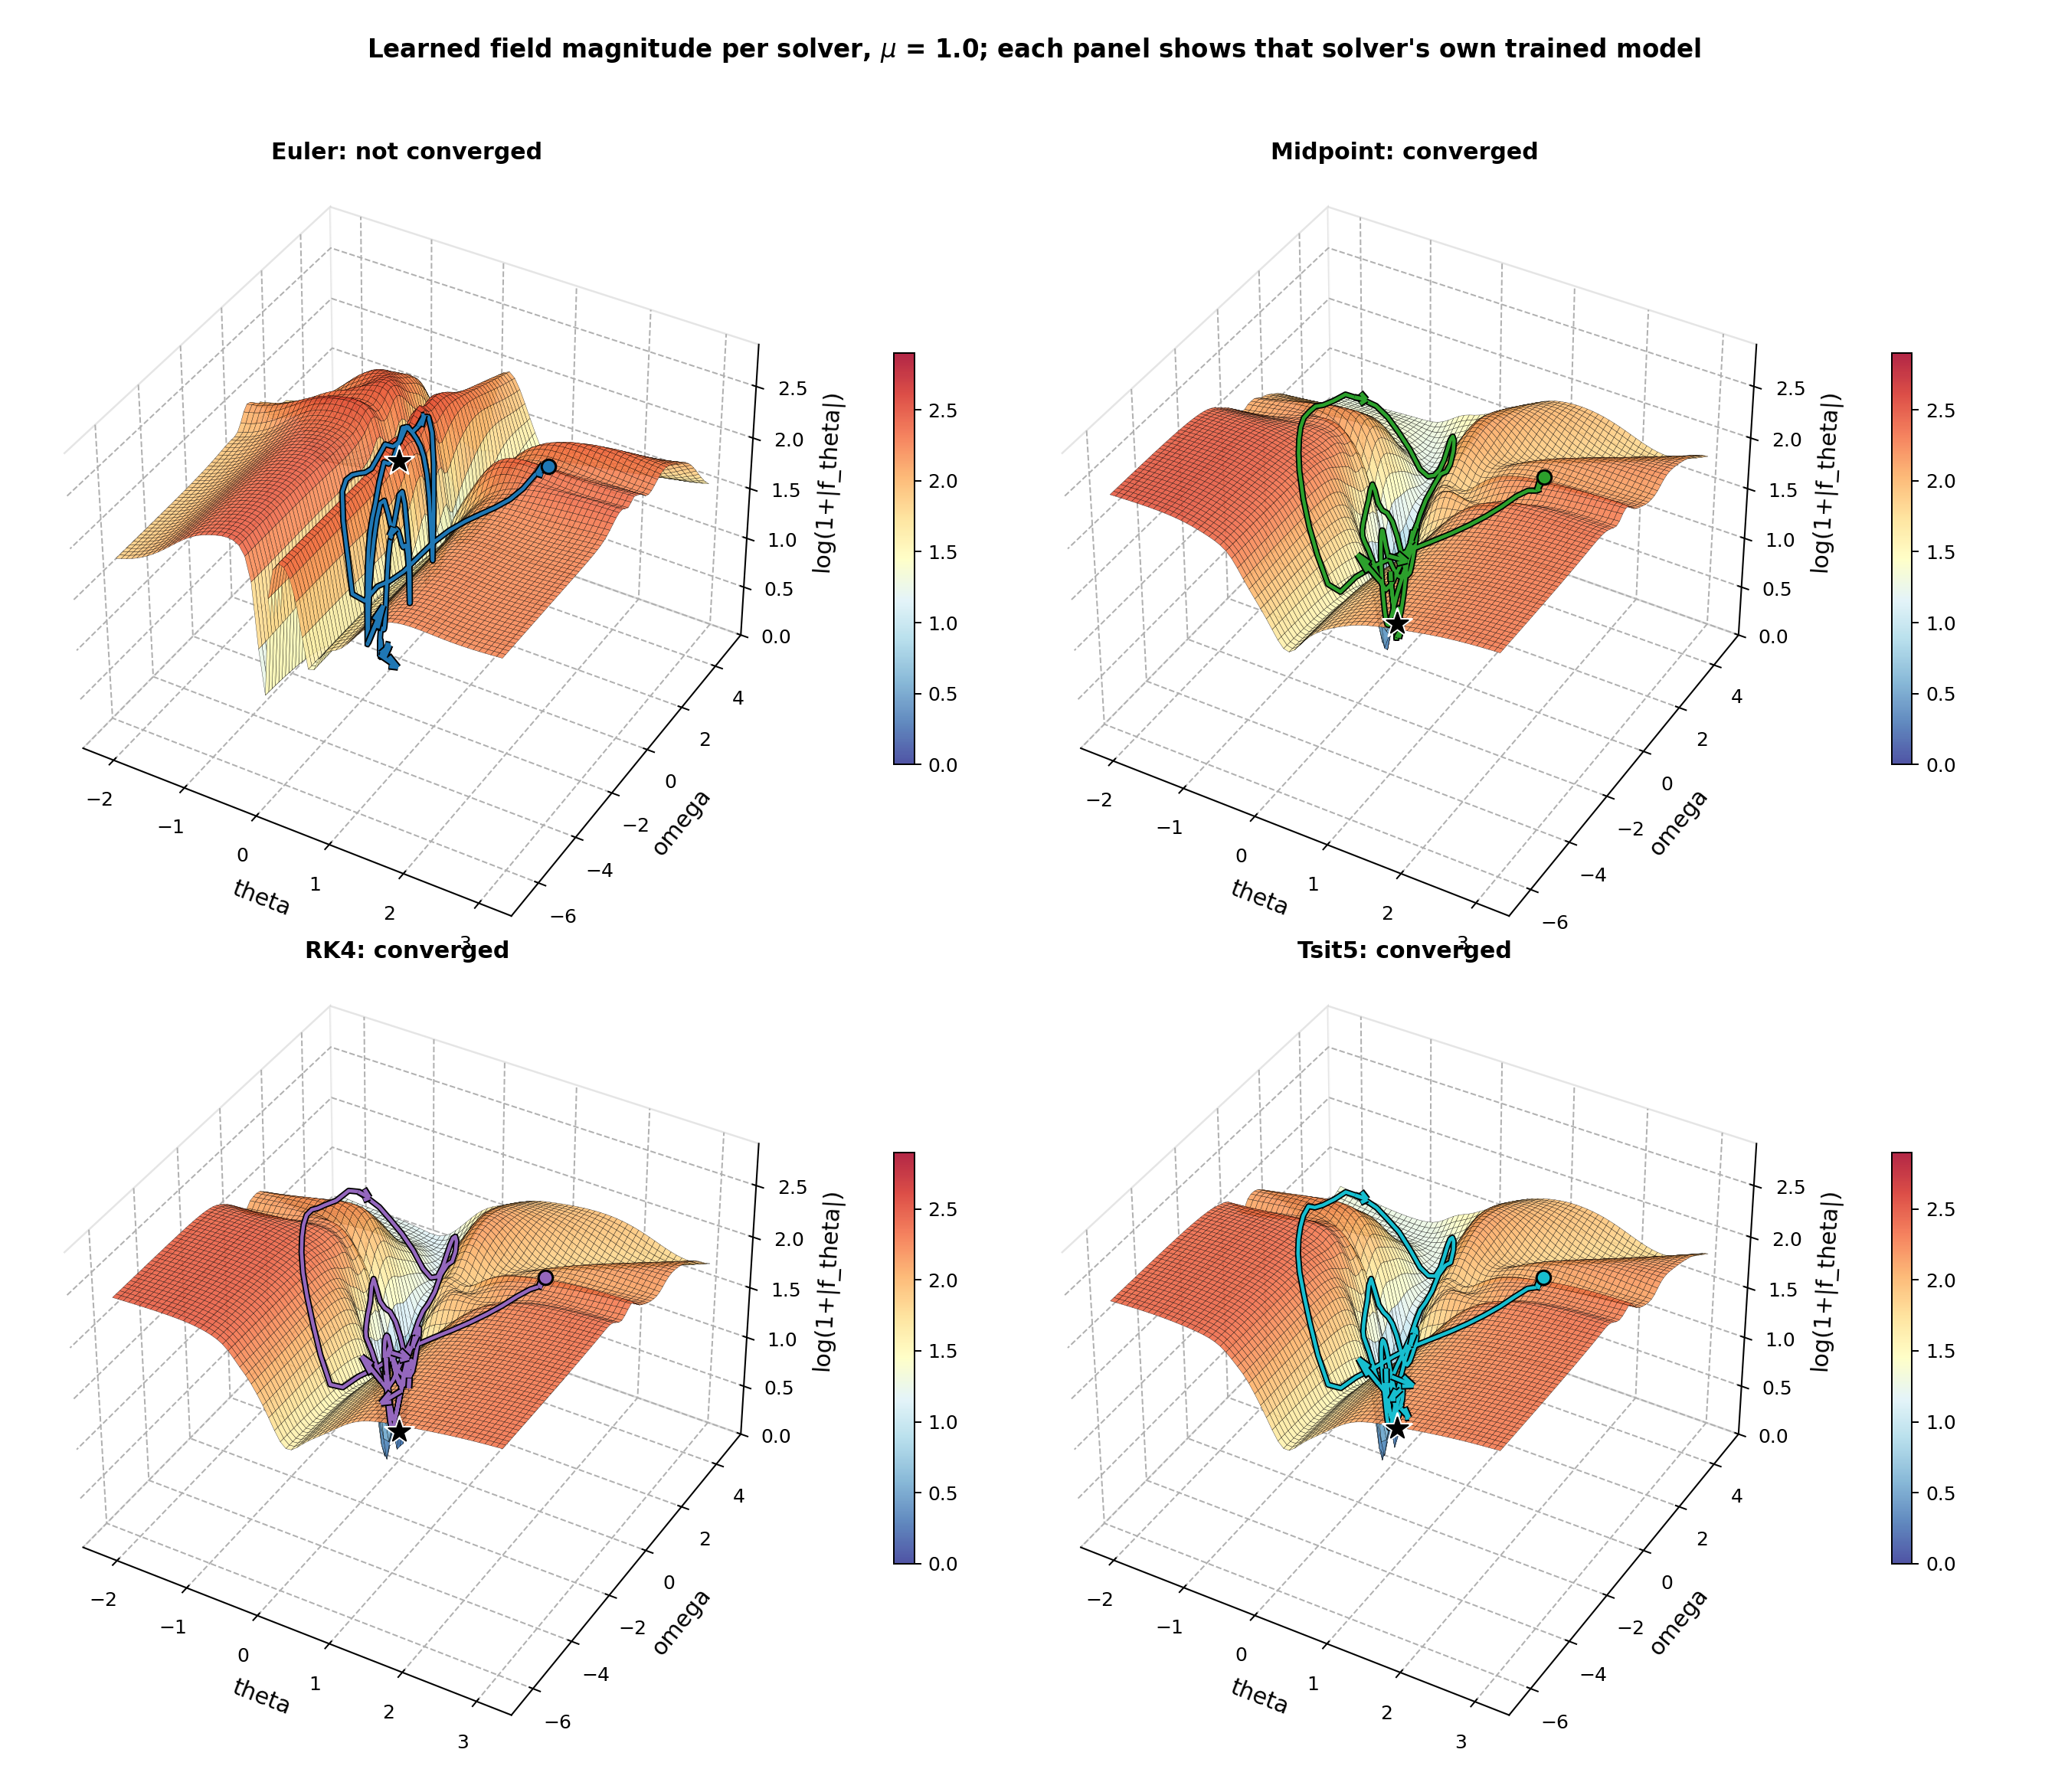
\includegraphics[width=\linewidth]{figures/track_d/phase_portrait_3d_mu1.0.png}
\end{minipage}
\caption{Learned vector-field landscape $|f_\theta(\theta,\omega)|$, per solver's
own trained model. Left ($\mu=2.0$): every solver's true equilibrium (star)
sits partway up a slope, while a separate, lower point nearby is where each
trajectory actually settles. Right ($\mu=1.0$): Euler's star sits high on a
ridge, well apart from where its trajectory spirals down and rests; for the
other three solvers, star and resting point coincide at the valley floor.}
\label{fig:phase-portraits}
\end{figure*}

The full predicted trajectories tell the same story over time rather than in
a single snapshot. Figure~\ref{fig:mu2-collage} shows every solver's
predicted angle, angular velocity, and error at $\mu=2.0$ settling onto the
same wrong, generic trajectory; Figure~\ref{fig:mu1-collage} shows the
$\mu=1.0$ case, where only Euler's predicted angle visibly departs from the
true one.

\begin{figure*}[t]
\centering
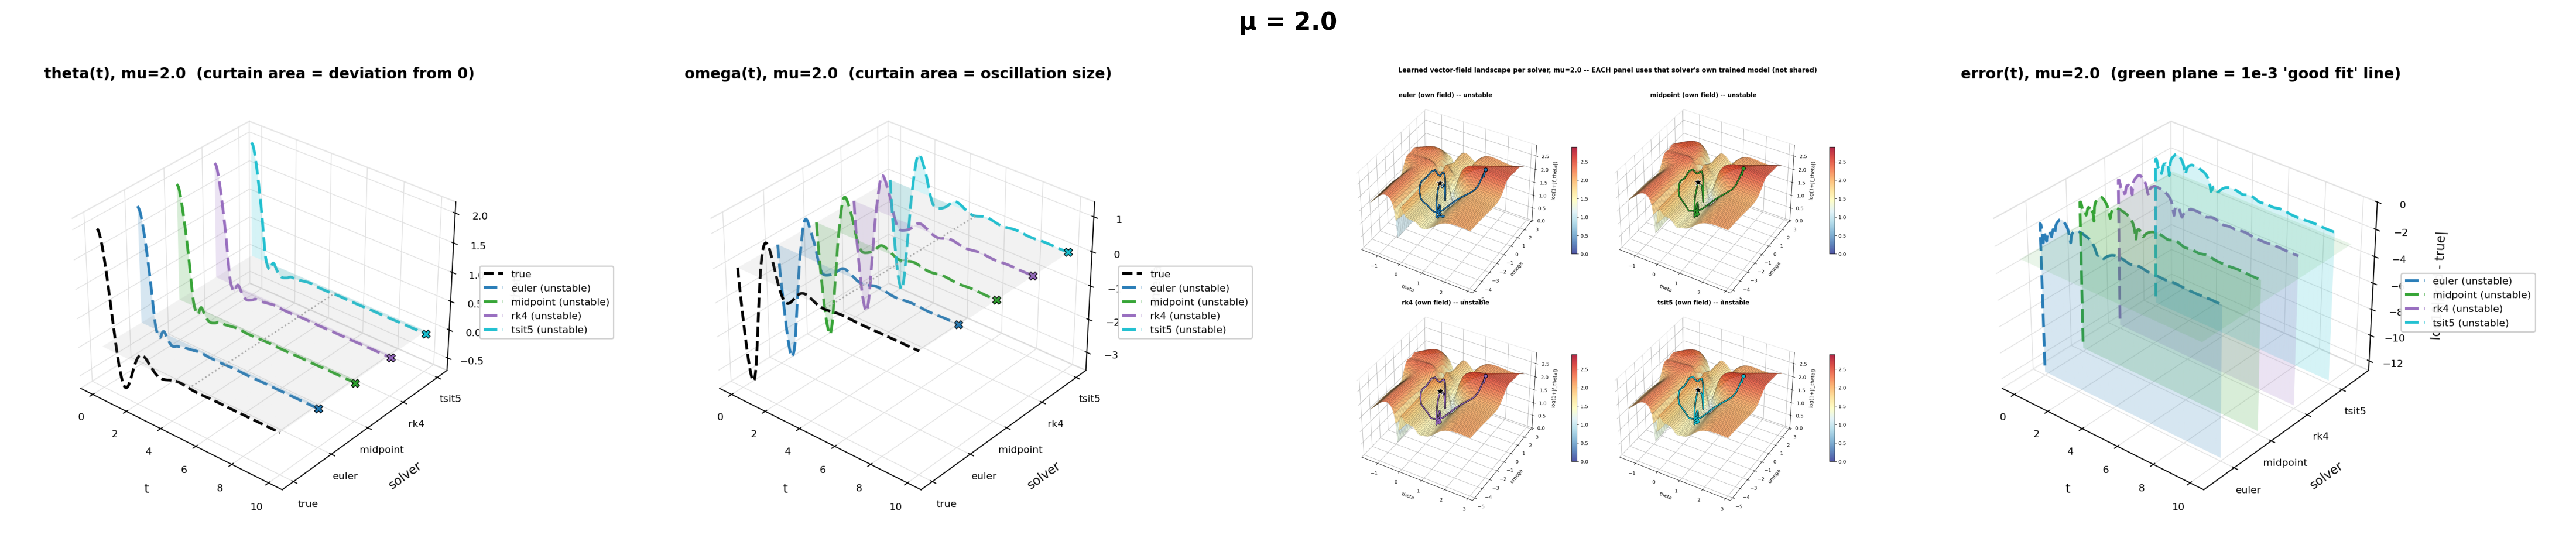
\includegraphics[width=\textwidth]{figures/track_d/mu2.0_trajectory_collage.png}
\caption{$\mu=2.0$, all four solvers: predicted angle, angular velocity, and
error over time, alongside each solver's phase portrait.}
\label{fig:mu2-collage}
\end{figure*}

\begin{figure*}[t]
\centering
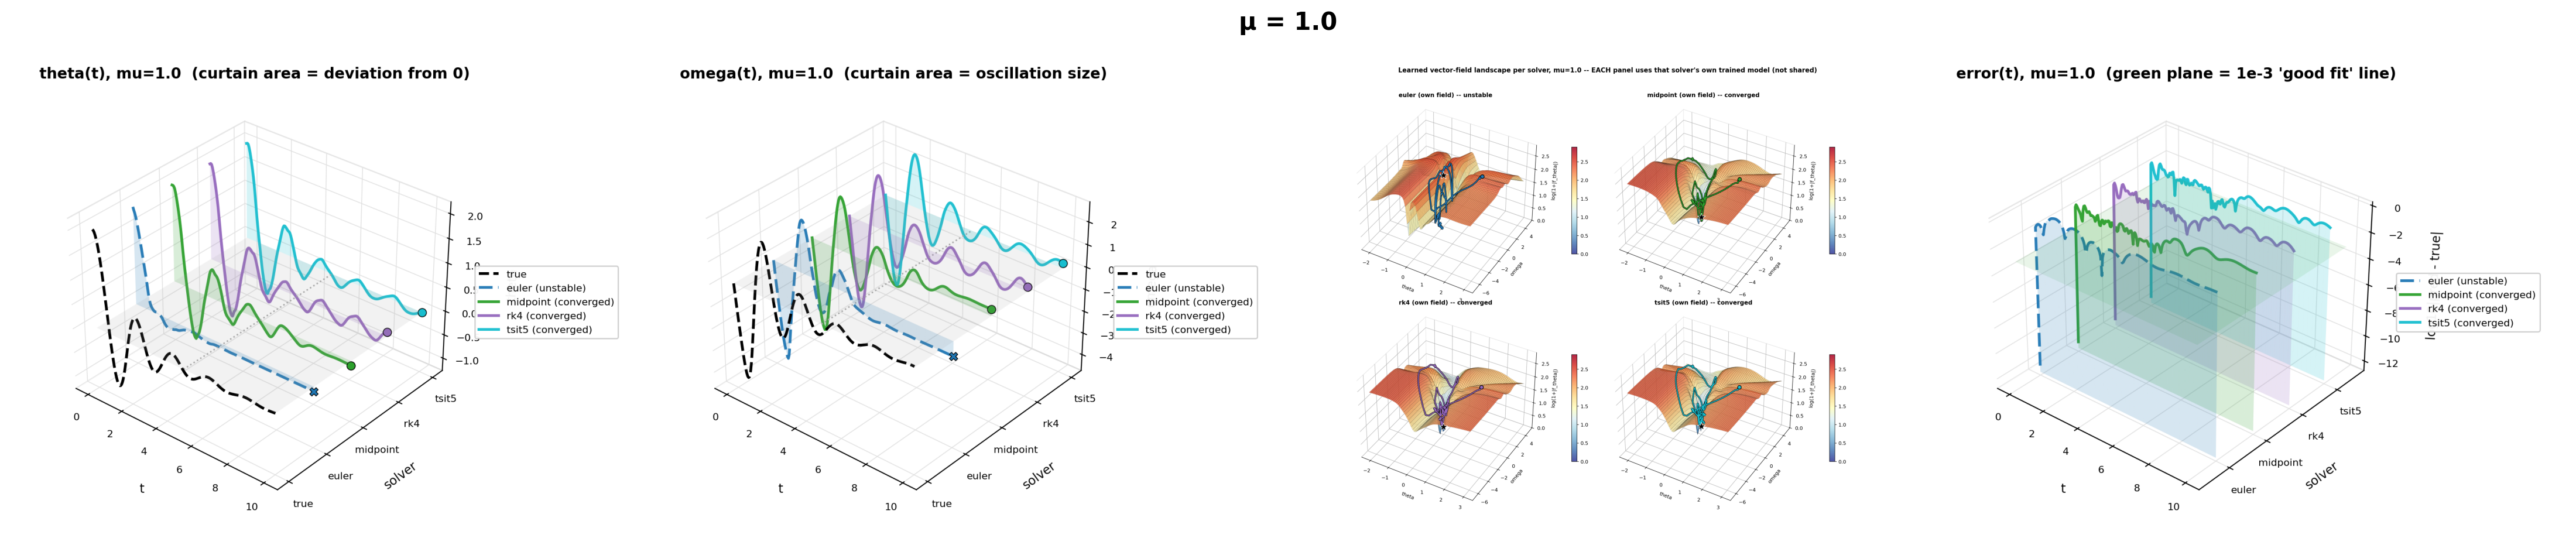
\includegraphics[width=\textwidth]{figures/track_d/mu1.0_trajectory_collage.png}
\caption{$\mu=1.0$, all four solvers: the same panel layout, showing Euler's
trajectory diverging from the true angle while the other three track it
closely.}
\label{fig:mu1-collage}
\end{figure*}

\subsubsection{Weight-space loss landscape: an independent measurement}

The phase-space plots above describe the learned dynamics. A separate
question is how forgiving the \emph{training loss} is around each solution:
does a small nudge to the weights leave the fit essentially unchanged, or
make it collapse? We measured this by stepping each trained model's weights
along two random directions and re-evaluating training error on a grid,
following the visualization technique of Li et al.\ \cite{li2018losslandscape}
adapted to KAN-ODE's 360-parameter weight space. Every cell traces the same
qualitative shape (a dip at the trained point that rises moving outward),
and we summarize each by its ``rise'': the number of orders of magnitude the
log-loss climbs by the edge of the grid.

\begin{table}[tb]
\centering
\small
\renewcommand{\arraystretch}{1.1}
\caption{Loss-landscape rise, single direction-pair (seed 0).}
\label{tab:rise-seed0}
\begin{tabularx}{\columnwidth}{@{}C{0.9cm} Y Y Y Y@{}}
\toprule
\hdrrow \thh{$\mu$} & \thh{euler} & \thh{midpoint} & \thh{rk4} & \thh{tsit5}\\
\midrule
1.0 & \textbf{5.53} & 9.03 & 8.99 & 9.12\\
2.0 & \textbf{4.23} & \textbf{4.24} & \textbf{4.22} & \textbf{4.20}\\
5.0 & 8.75 & 8.75 & 8.76 & 8.76\\
8.0 & 9.14 & 9.15 & 9.12 & 9.12\\
\bottomrule
\end{tabularx}
\end{table}

The converged models (rise $\approx9$) sit at the bottom of a narrow, steep
basin: stepping even a small distance from the trained weights in either
random direction drives the log-loss up by nine orders of magnitude, so the
surrounding terrain looks like a sharp valley with the solution pinned at its
floor. The trapped cells (bold, rise $\approx4$--$5.5$) sit in a basin roughly
half as steep. The terrain around them is closer to a broad, gently sloped
plain than a valley, and the same size step barely raises the loss by
comparison. This is the opposite of the usual intuition that a flat minimum
generalizes better. Here, the flat region is where training settled for a
generic, low-effort answer, and the steep, narrow basin is where it actually
learned the pendulum's dynamics.

Figure~\ref{fig:landscape-mu2-euler} renders this directly as a surface. The
terrain around Euler's trapped $\mu=2.0$ solution is a broad, gently rolling
plain with no sharply defined bottom. This contrasts clearly with
Figure~\ref{fig:landscape-mu1-tsit5}'s converged $\mu=1.0$ solution, which
sits at the bottom of a narrow, sharply walled valley; it is the same
contrast the rise numbers above report as a factor of roughly two, made
visible. Figure~\ref{fig:landscape-mu1-euler} shows the trapped $\mu=1.0$
case under the same solver whose $\mu=2.0$ terrain is shown alongside it,
confirming the flat terrain is a property of the trapped solution rather than
of any one damping value.

\begin{figure*}[t]
\centering
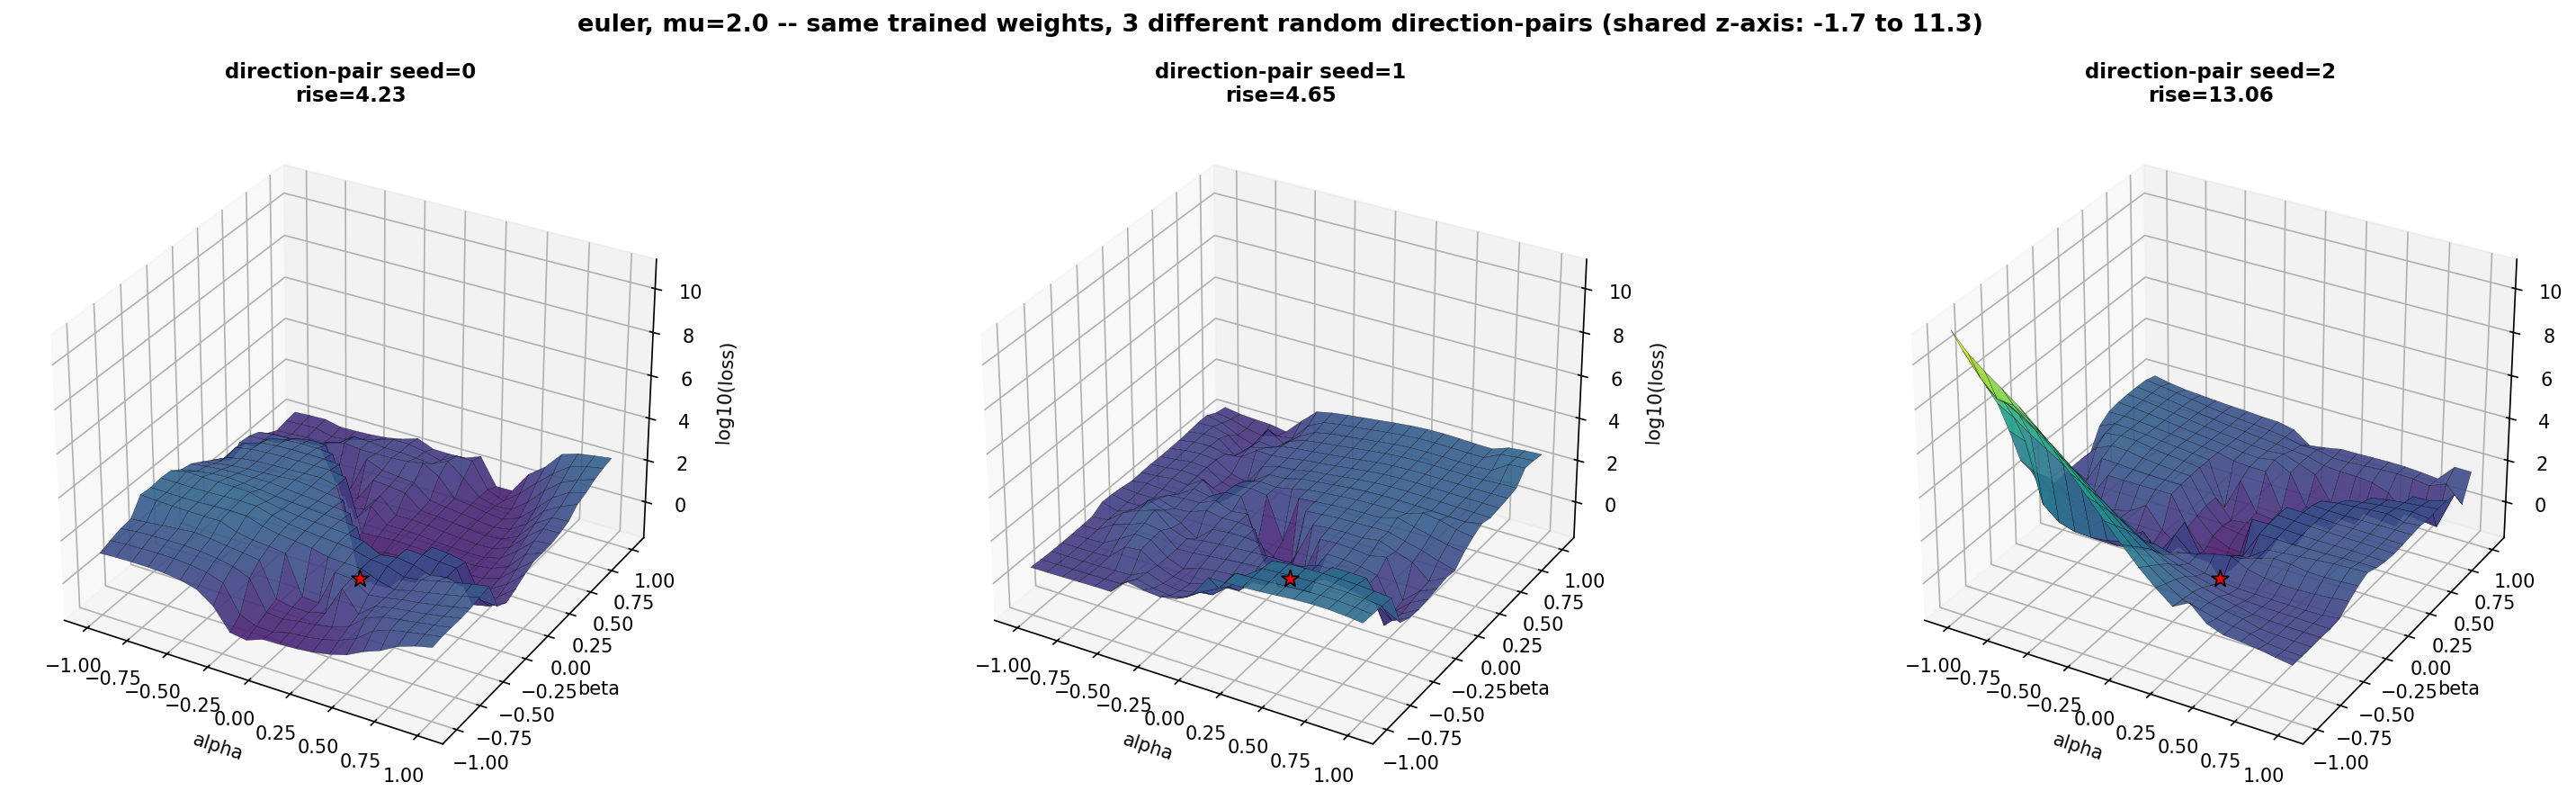
\includegraphics[width=0.75\textwidth]{figures/track_d/mu2.0_euler_direction_comparison.png}
\caption{Euler, $\mu=2.0$ (trapped): the training-loss surface around the
trained weights, viewed under three independent random direction-pairs. The
basin near the trained point (the marked star) is broad and shallow in all
three views; the third panel's steep spike on the far side is the outlier
direction discussed below, not the basin itself.}
\label{fig:landscape-mu2-euler}
\end{figure*}

\begin{figure*}[t]
\centering
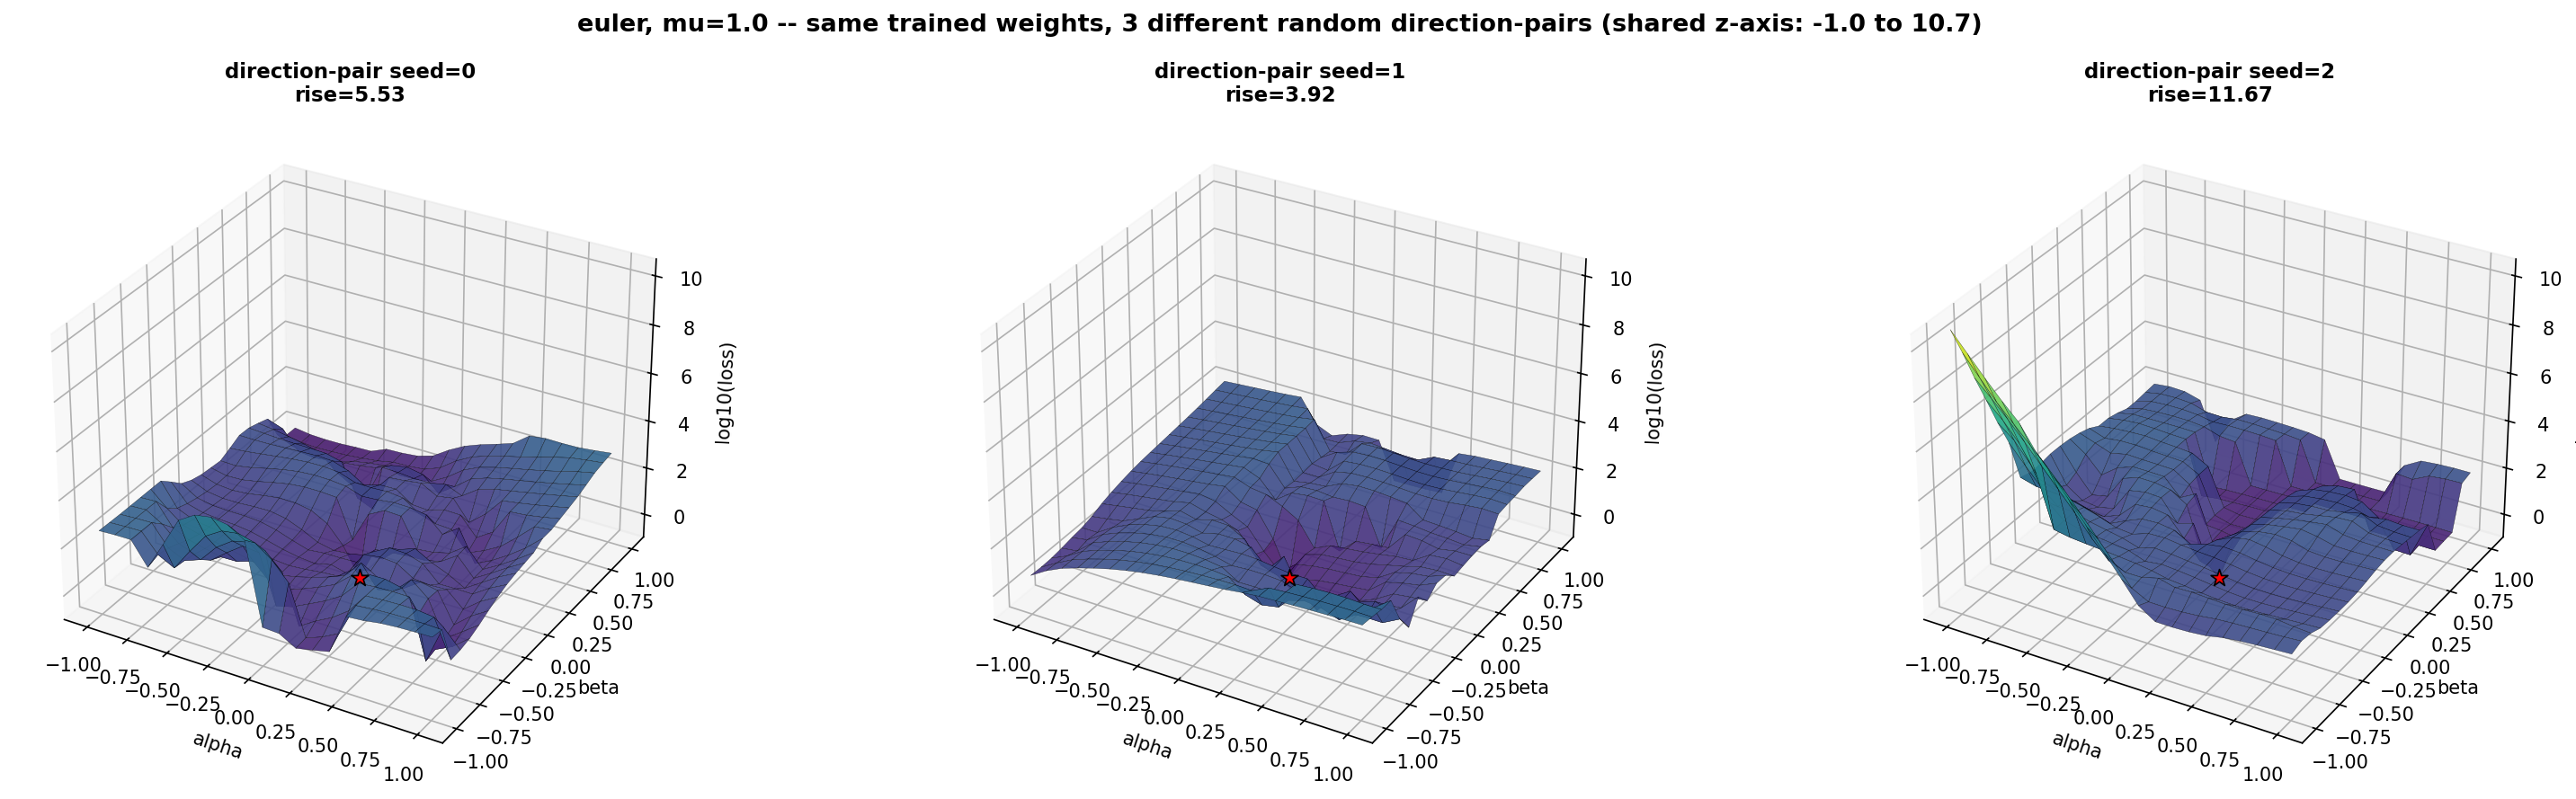
\includegraphics[width=0.75\textwidth]{figures/track_d/mu1.0_euler_direction_comparison.png}
\caption{Euler, $\mu=1.0$ (also trapped): the same broad, shallow basin shape
recurs at a different damping value under the same solver.}
\label{fig:landscape-mu1-euler}
\end{figure*}

\begin{figure*}[t]
\centering
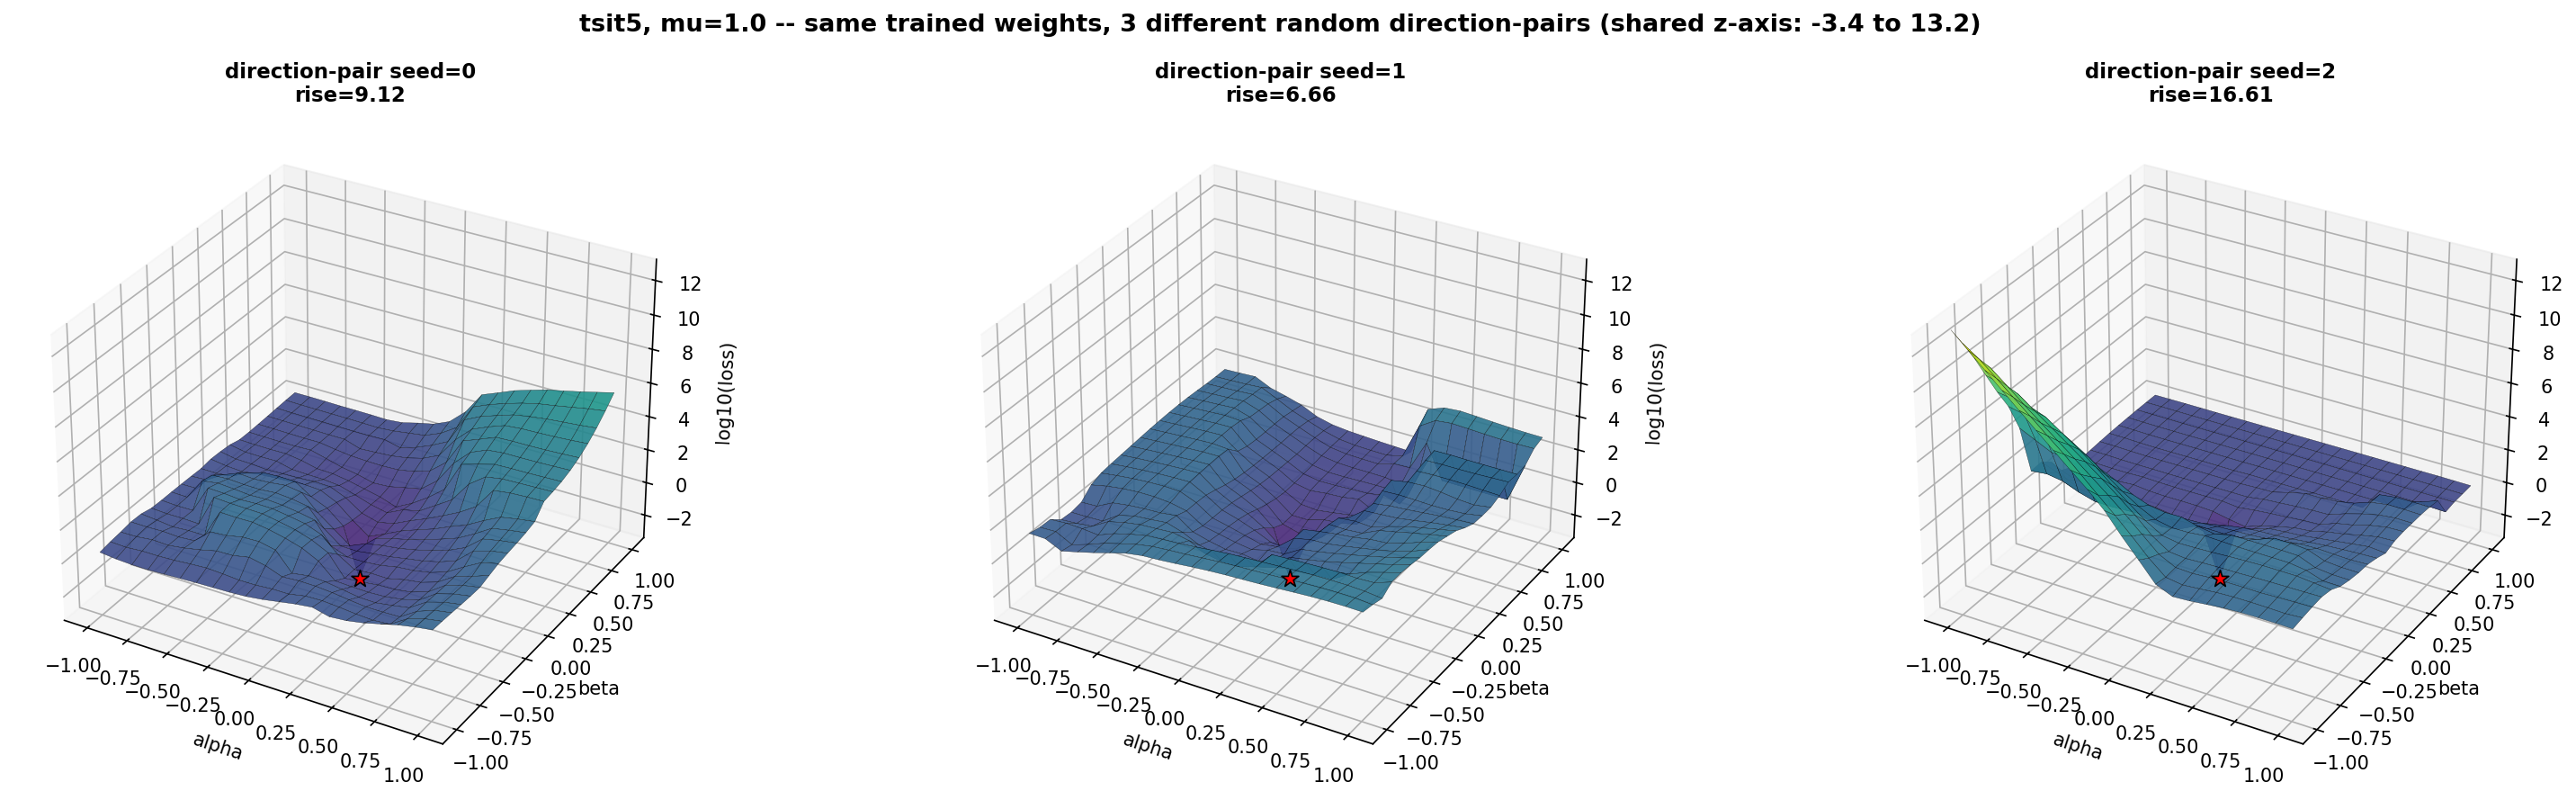
\includegraphics[width=0.75\textwidth]{figures/track_d/mu1.0_tsit5_direction_comparison.png}
\caption{Tsit5, $\mu=1.0$ (converged): the basin around the trained point is
visibly narrower and drops noticeably lower, in every one of the three
direction-pairs, than either trapped case above.}
\label{fig:landscape-mu1-tsit5}
\end{figure*}

\paragraph{Robustness check across three direction-pairs.} Repeating the
measurement with two more independent random direction pairs per cell (72
measurements total) found one direction-pair acting as a shared outlier
across nearly every cell. Because every model shares the same architecture,
one particular raw random draw runs toward a steeper wall in all 24 cells at
once, inflating that direction's rise by roughly $2$--$3\times$ everywhere.
The size of the measured effect depends on how many direction choices are
averaged. The single-seed $\approx2\times$ gap between trapped and converged
cells narrows to roughly 20--30\% once all three direction-pairs are
averaged, since the outlier direction inflates the trapped cells' mean more
than the converged cells' mean. The ranking between cells holds regardless;
only the apparent size of the gap changes. The multi-seed average is the
figure to trust; the single-seed table above illustrates the shape of the
effect at a scale that is easier to see.

\begin{figure*}[t]
\centering
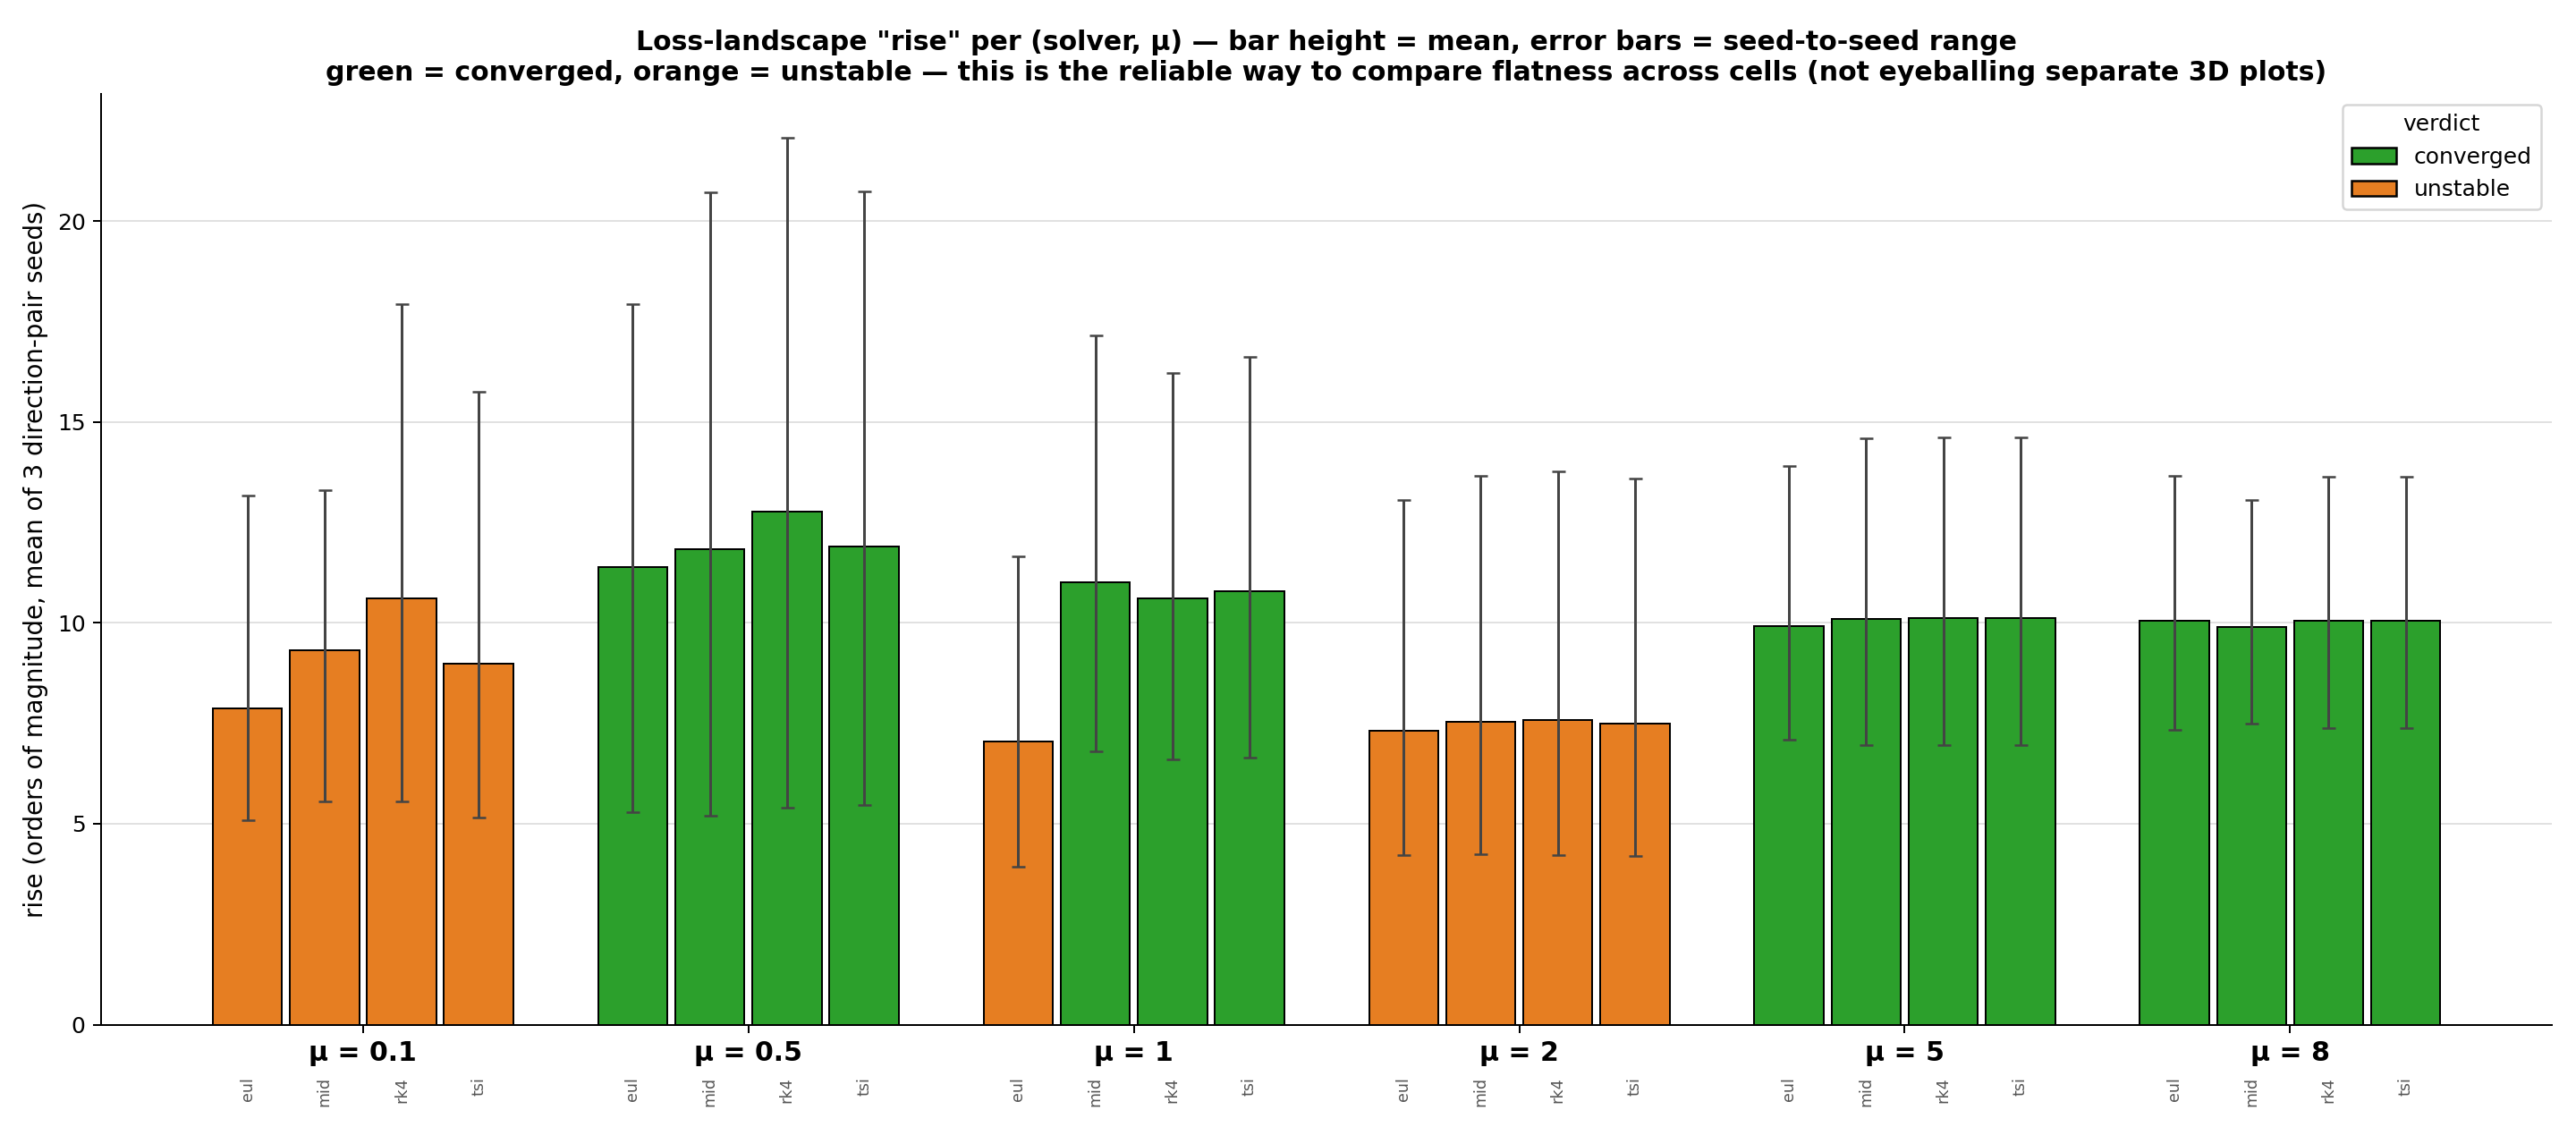
\includegraphics[width=0.65\textwidth]{figures/track_d/rise_comparison_bars.png}
\caption{Mean rise per (solver, $\mu$), 3-seed average with seed-to-seed range
as error bars, colored by verdict.}
\label{fig:rise-bars}
\end{figure*}

The cells trapped by the spurious-equilibrium mechanism ($\mu=2.0$ across
all solvers, and Euler's own $\mu=1.0$) sit around 20--30\% lower on this
chart than converged cells: a modest but measured gap rather than an
order-of-magnitude separation. $\mu=0.1$ carries the ``unstable'' label for
an unrelated reason: its trajectory never settles within the training window
at all, and its bars sit in the same range as the converged
$\mu\in\{5.0,8.0\}$ cells, occasionally above them. The flatness effect
belongs specifically to the spurious-equilibrium trap cases, and does not
generalize to every cell the pipeline labels ``unstable.''

\begin{figure*}[t]
\centering
\begin{minipage}[t]{0.36\textwidth}
\centering
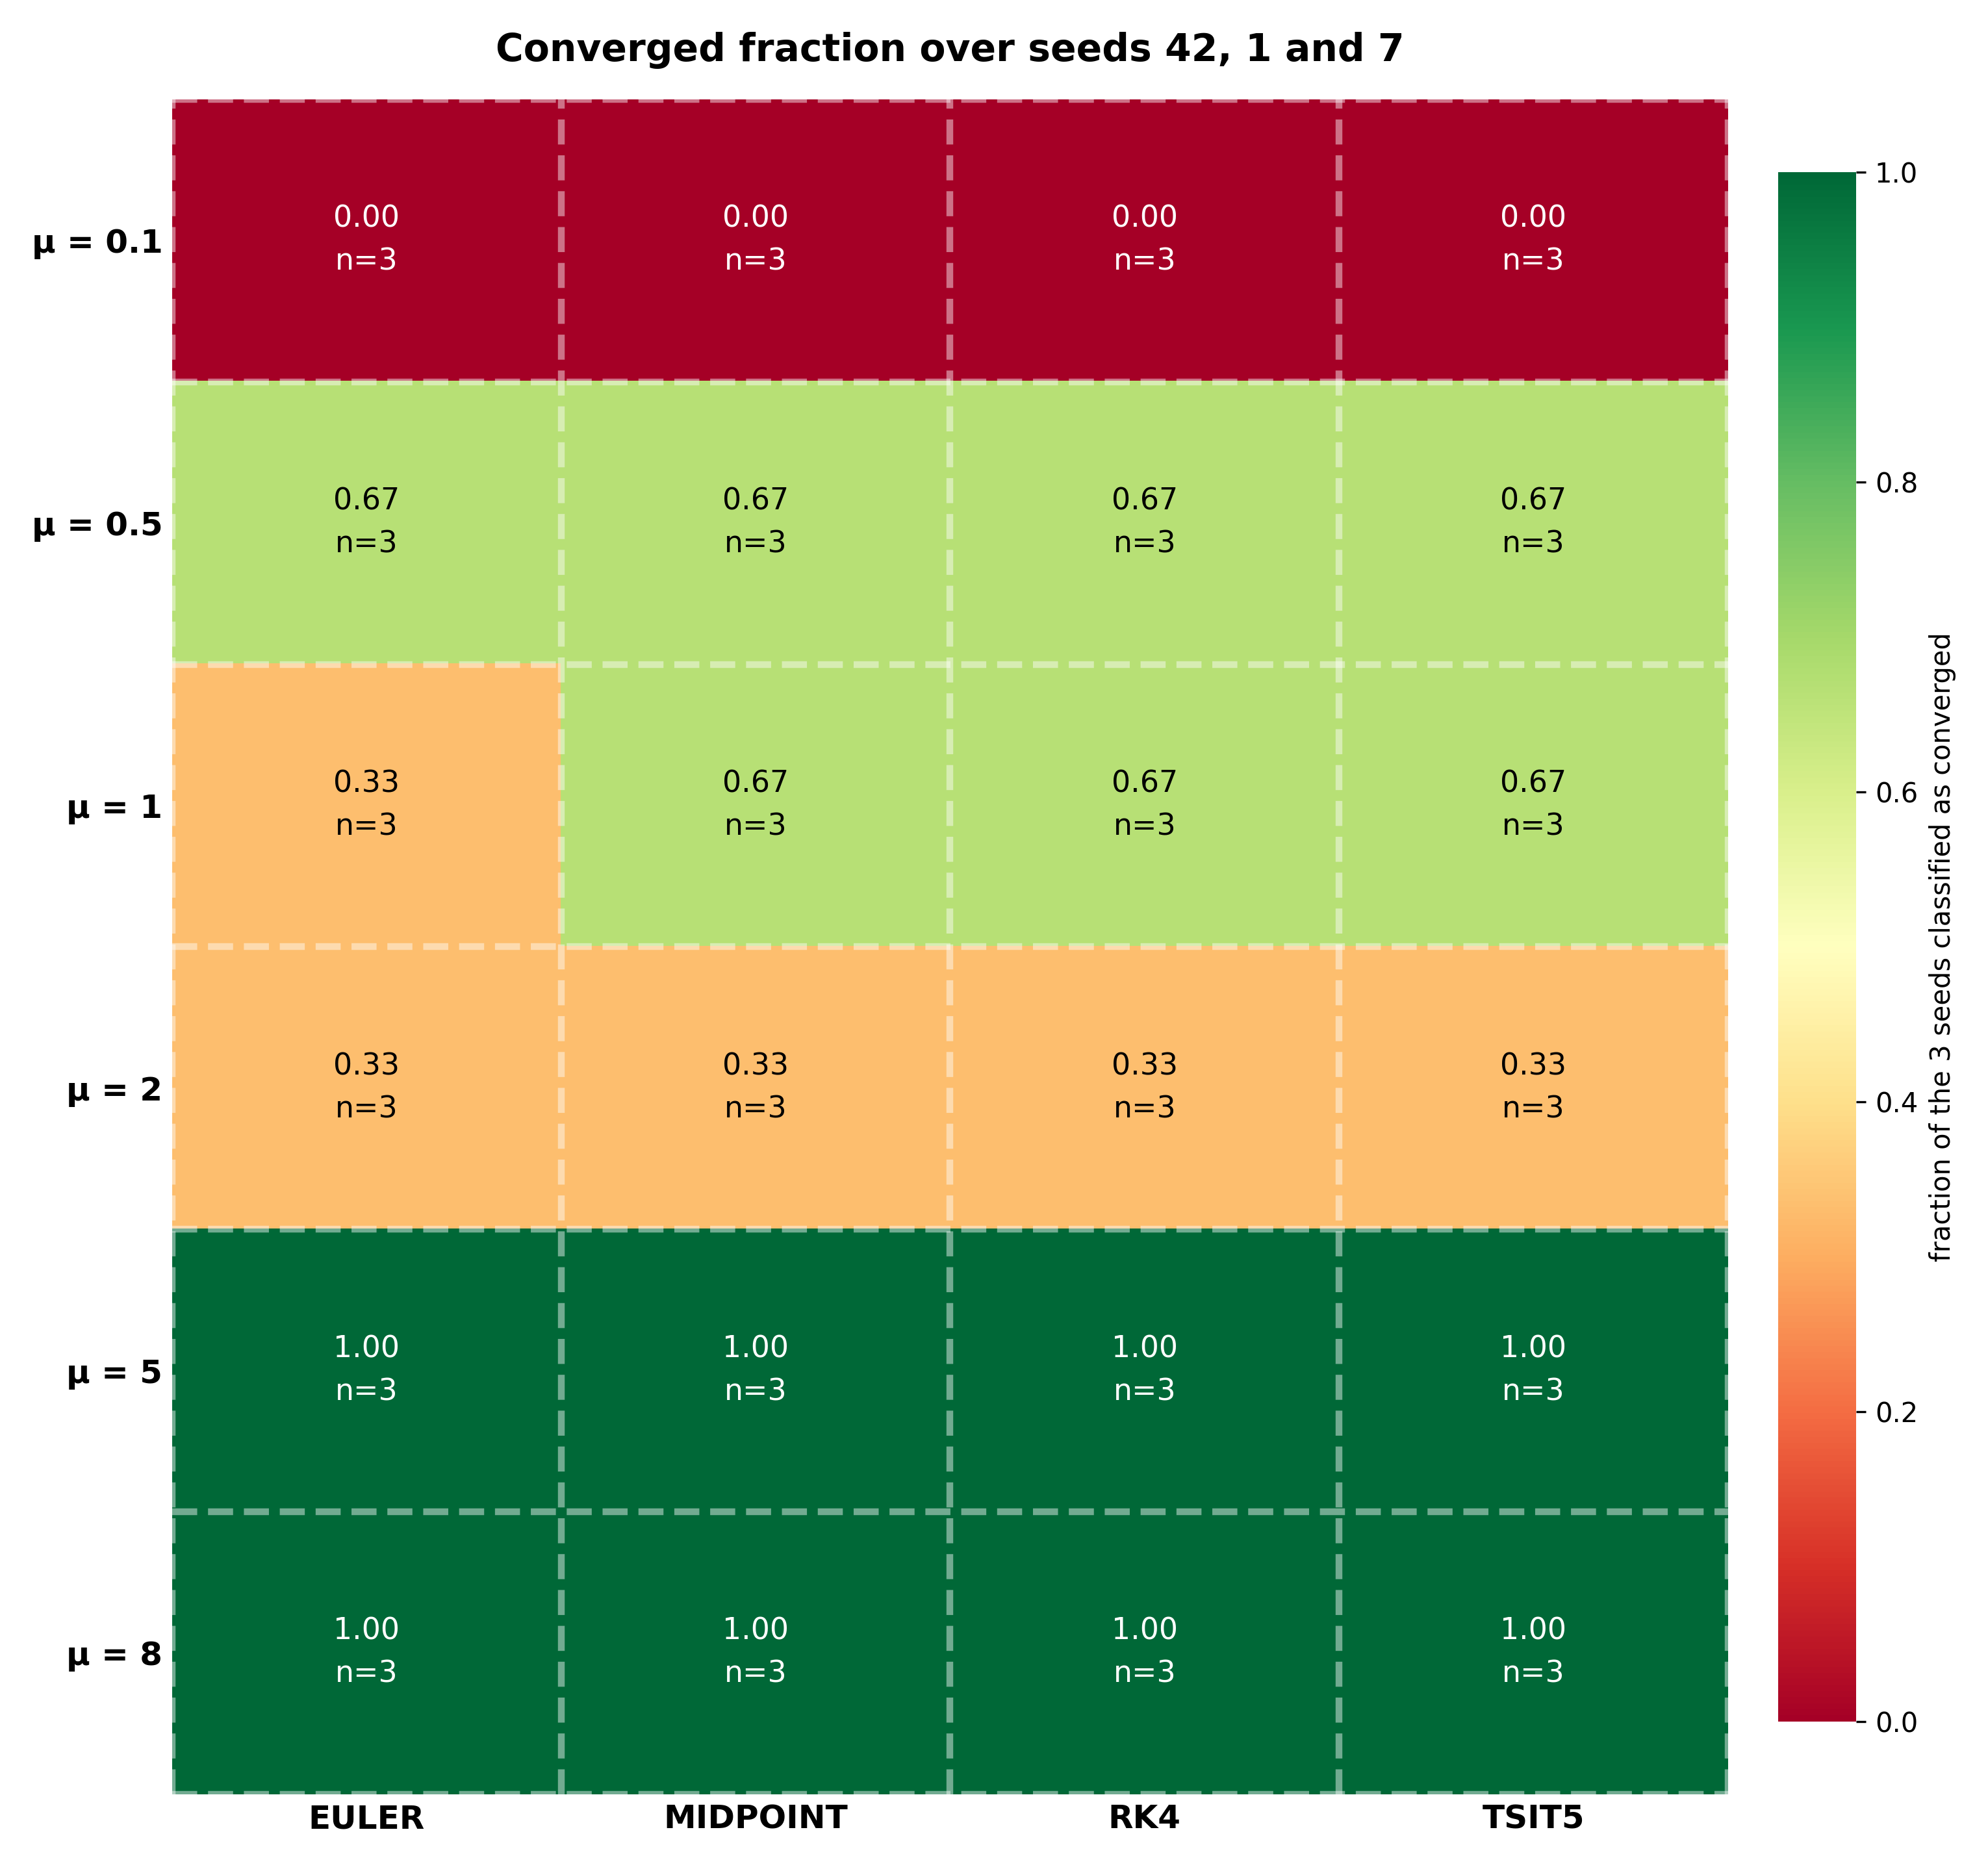
\includegraphics[width=\linewidth]{figures/track_d/seed_converged_fraction_heatmap.png}
\end{minipage}\hspace{0.04\textwidth}
\begin{minipage}[t]{0.36\textwidth}
\centering
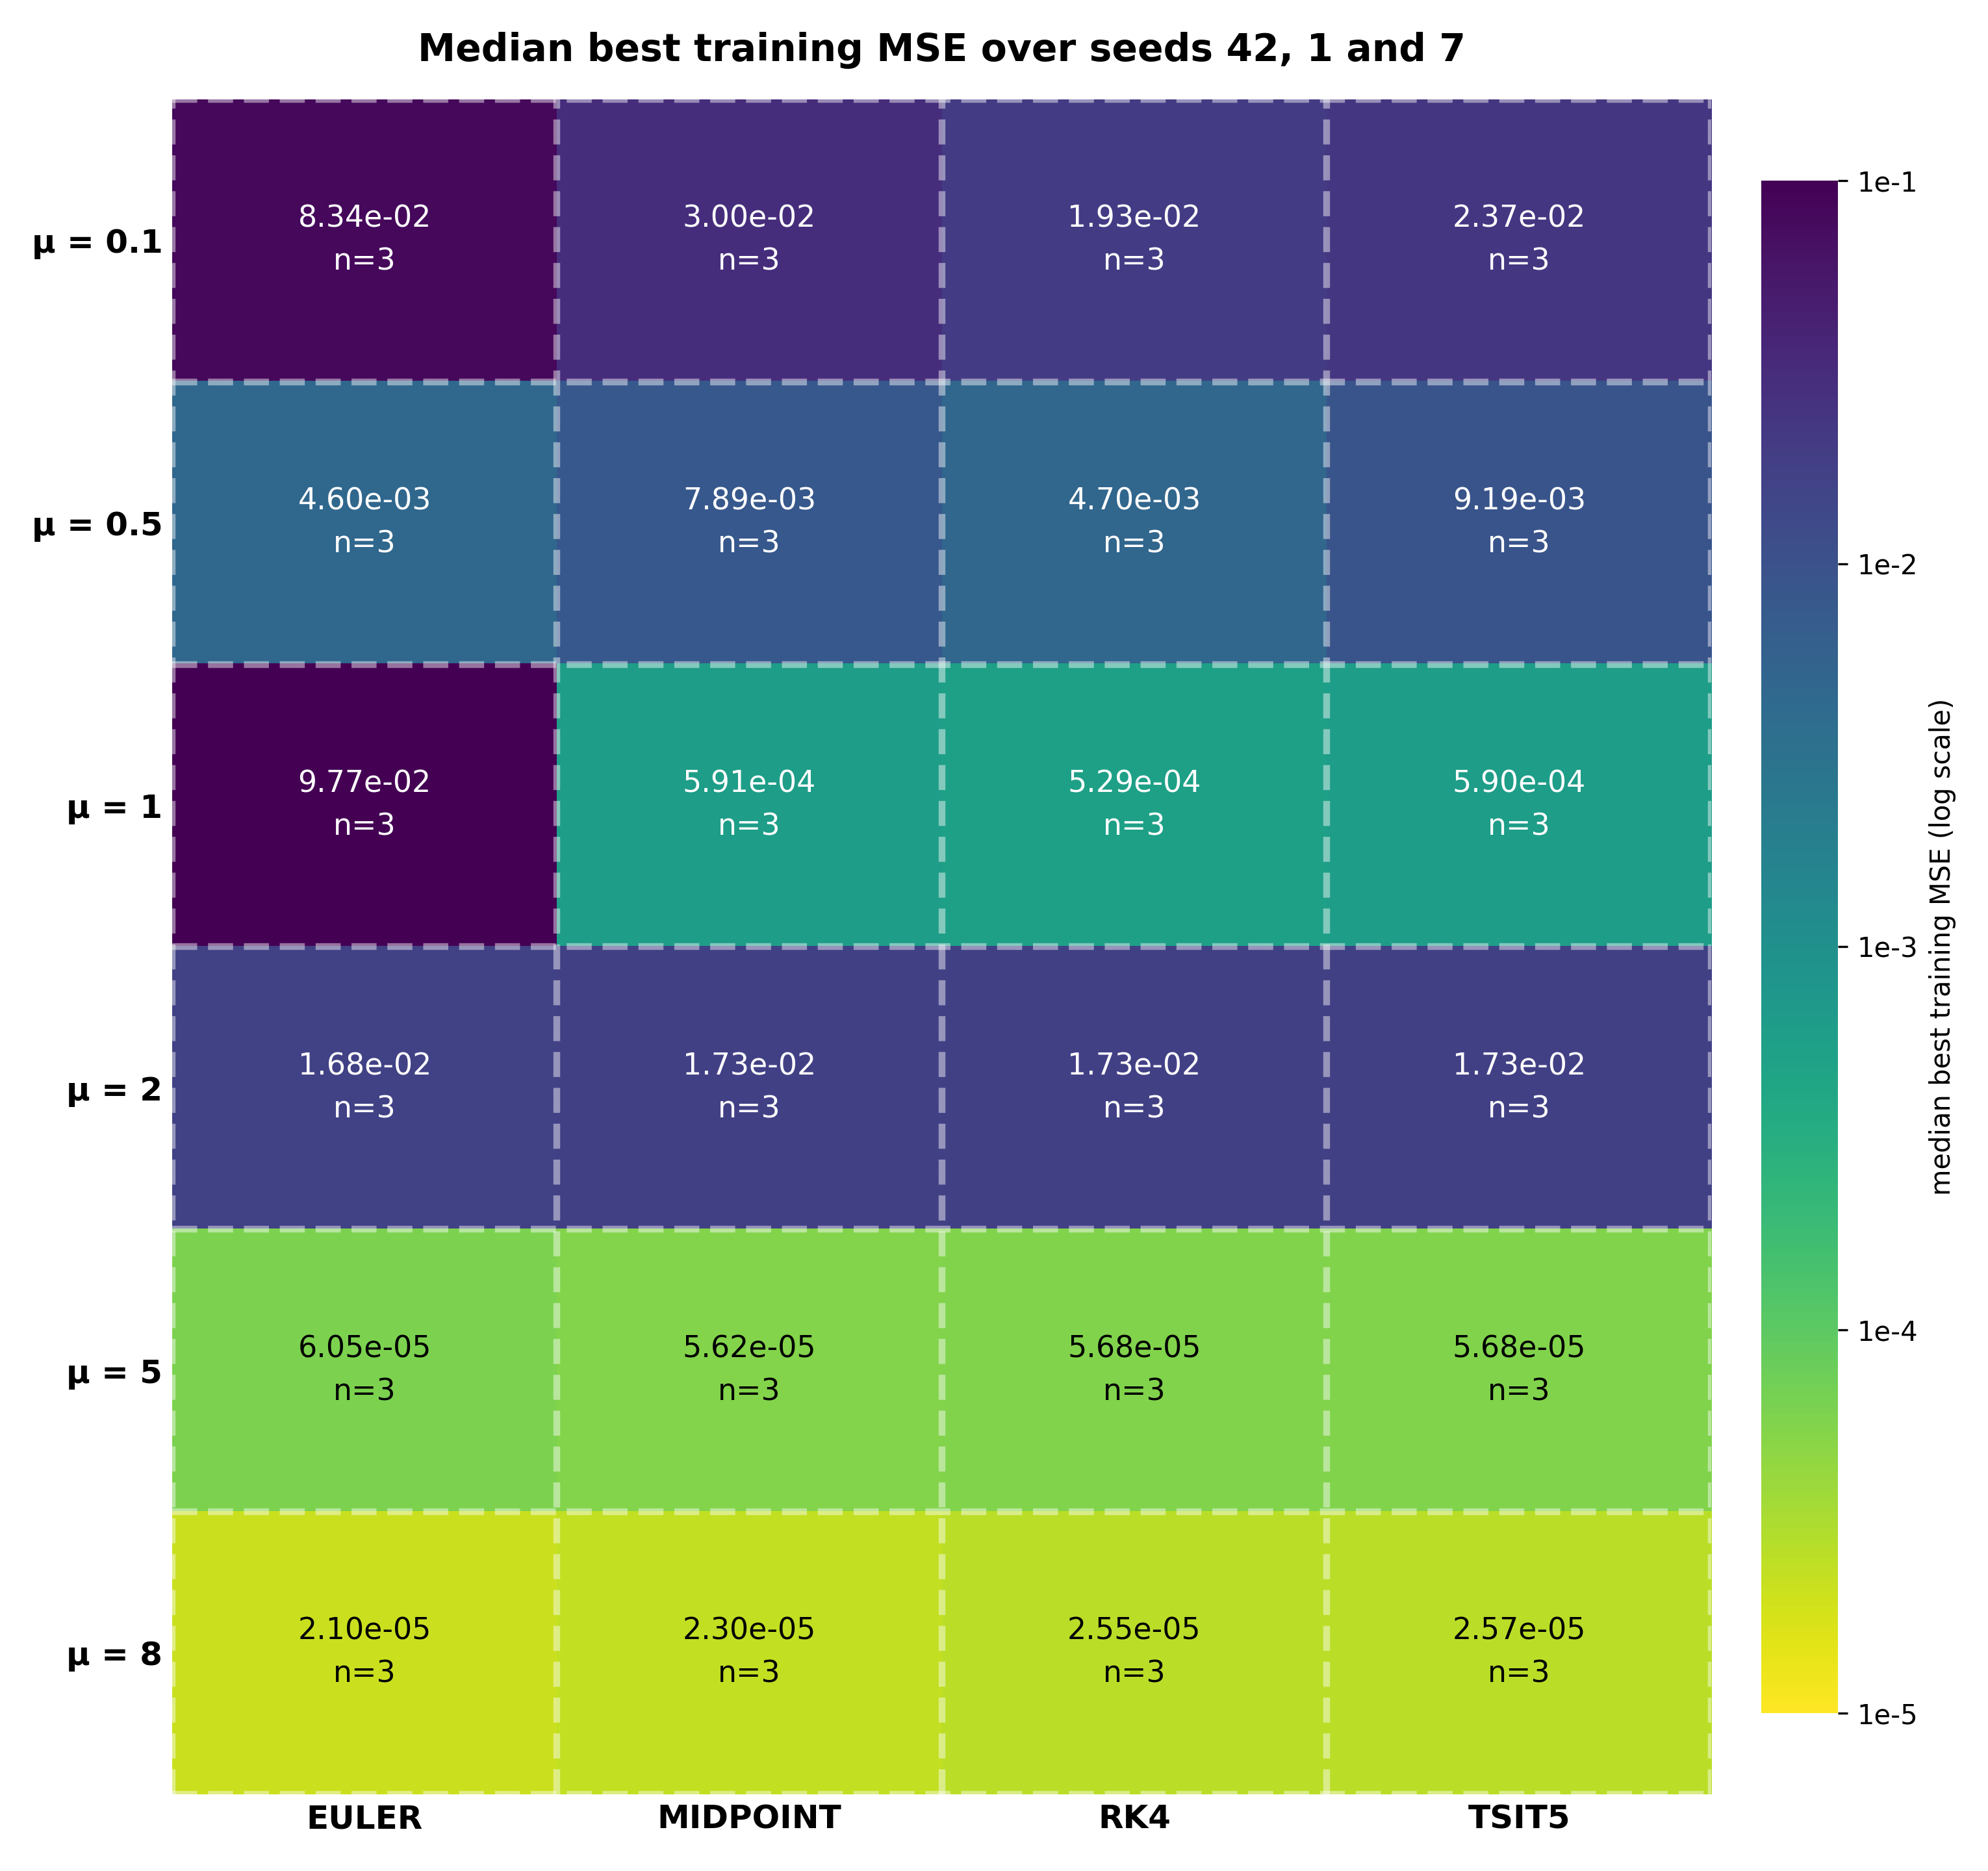
\includegraphics[width=\linewidth]{figures/track_d/seed_median_mse_heatmap.png}
\end{minipage}
\caption{Converged fraction (left) and median training MSE (right) over 3
seeds, all 4 solvers $\times$ 6 $\mu$ (72 cells). The two agree everywhere:
low converged-fraction cells are exactly the cells with elevated median
error.}
\label{fig:seed-converged-fraction}
\end{figure*}

\begin{keypoint}[Verdict]
Every divergence-free prediction from linear stability theory held exactly,
so nothing in this sweep is a classical numerical-stiffness failure. The
mechanism at work is a seed-dependent local minimum in a 360-parameter
optimization landscape, producing a genuine, solver-independent spurious
equilibrium in the learned dynamics. Three independent lines of evidence
converge on this: per-solver trained-weight evaluation, phase-space
vector-field visualization, and an independently-measured, direction-robust
weight-space loss landscape.
\end{keypoint}

\subsection{Sparse regression and transfer to an outbreak curve}
\label{sec:track-e}

Here we compare two very different ways of discovering governing equations
from data: sparse symbolic regression and gradient-based neural fitting. We
also test separately whether the cross-domain stability fixes of
Section~\ref{sec:crossdomain} generalize beyond the mechanistic system that
produced them.

\subsubsection{Noise robustness: KAN-ODE vs.\ sparse symbolic regression}

We fit SINDy (Section~\ref{sec:sparse-method}) to the same noise-corrupted
Lotka-Volterra observations that the noise-sweep checkpoints
(Section~\ref{sec:dt-noise}) were trained on, and score both methods against
clean ground truth.

\begin{expectbox}
\expectrow{Question}{How does a sparse, symbolic method compare to a dense, 240-parameter neural method as observation noise increases?}
\expectrow{Expected}{Sparse regression's tiny library should make it more robust to noise; KAN-ODE's larger parameter count should make it more accurate.}
\expectrow{Observed}{Both expectations hold, but the KAN-ODE advantage collapses $170\times$ across the sweep, from $1110\times$ at zero noise to $6.5\times$ at $\sigma=0.1$.}
\end{expectbox}

\begin{table}[t]
\centering
\footnotesize
\renewcommand{\arraystretch}{1.1}
\caption{Extrapolation MSE vs.\ observation noise $\sigma$.}
\label{tab:sindy-noise}
\begin{tabularx}{\columnwidth}{@{}C{1.2cm} C{2.1cm} C{2.1cm} Y@{}}
\toprule
\hdrrow \thh{Noise level $\sigma$} & \thh{Sparse regression} & \thh{KAN-ODE} & \thh{KAN-ODE advantage}\\
\midrule
0.00 & $9.90\times10^{-2}$ & $\mathbf{8.92\times10^{-5}}$ & $1110\times$\\
0.01 & $1.58\times10^{-1}$ & $1.22\times10^{-3}$ & $130\times$\\
0.05 & $1.48\times10^{-1}$ & $2.54\times10^{-2}$ & $5.8\times$\\
0.10 & $8.89\times10^{-1}$ & $1.37\times10^{-1}$ & $6.5\times$\\
\bottomrule
\end{tabularx}
\end{table}

\begin{figure*}[t]
\centering
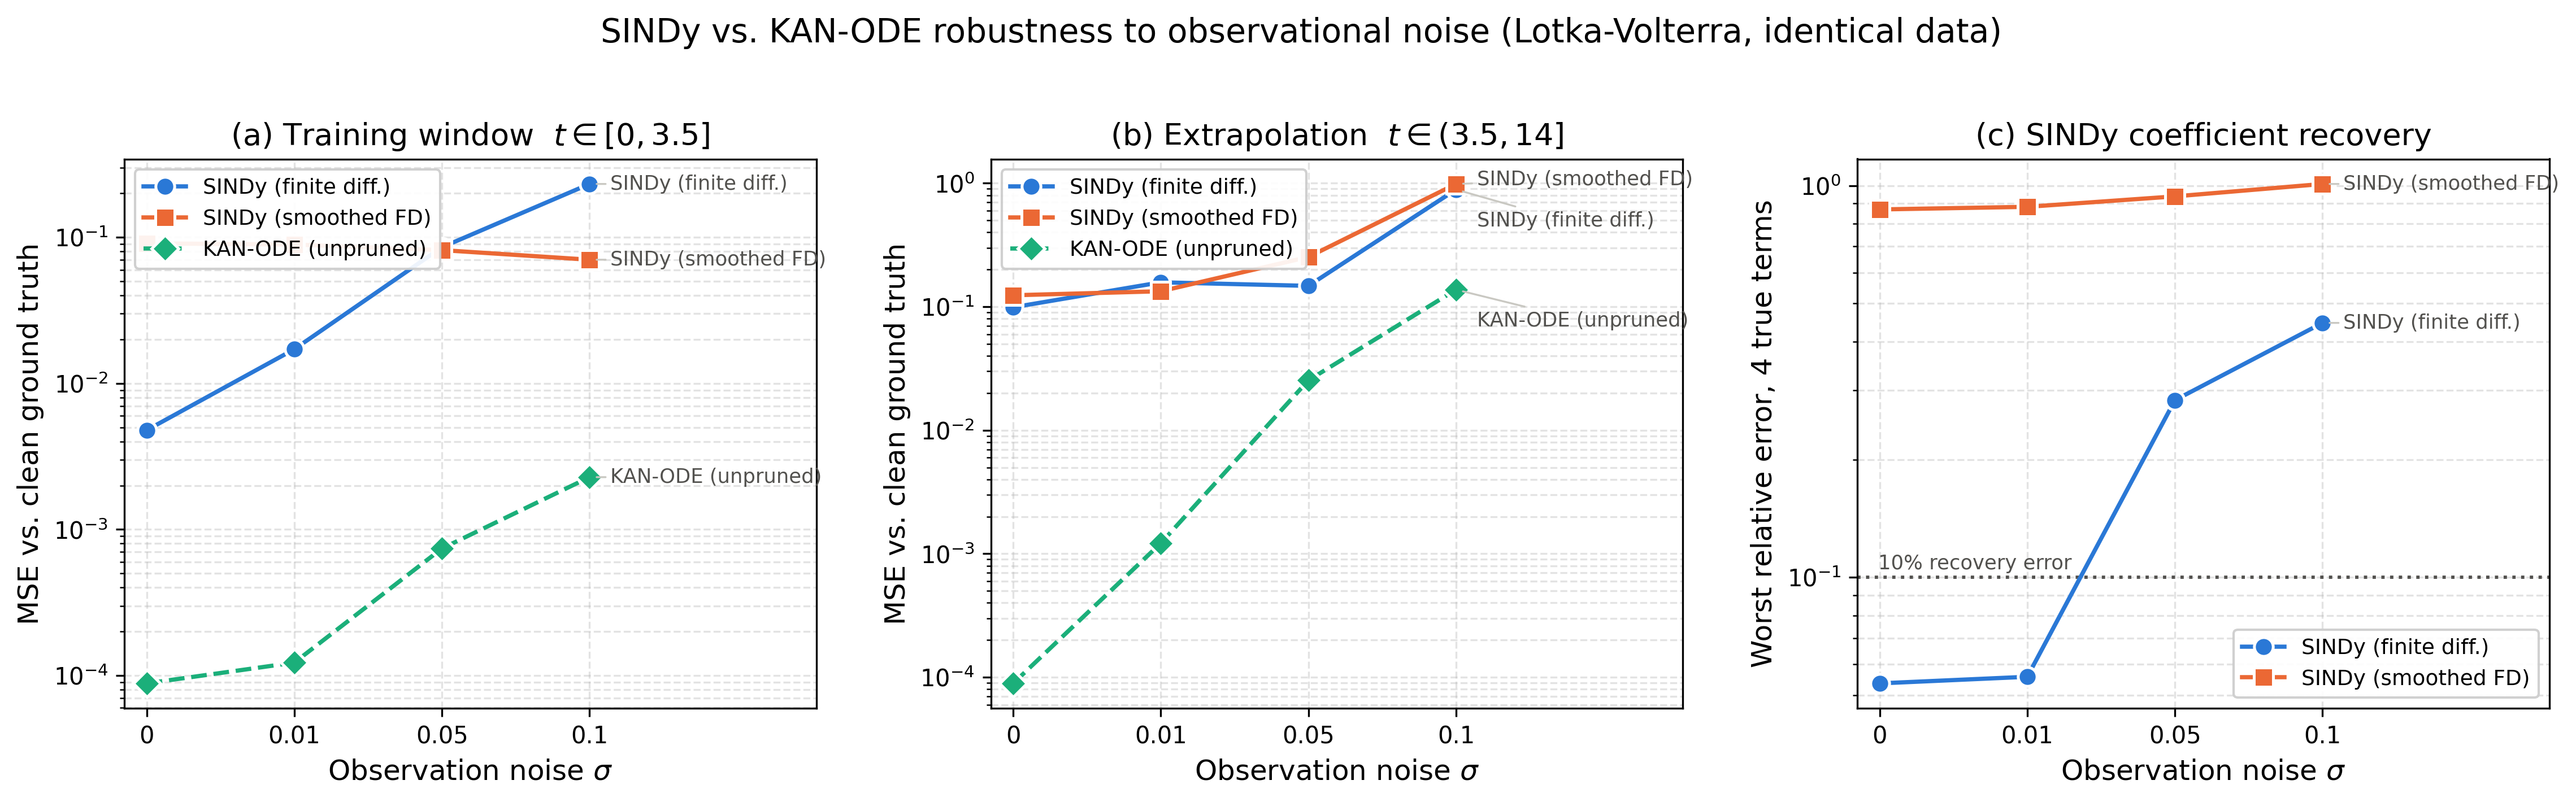
\includegraphics[width=0.85\textwidth]{figures/track_e/sindy_vs_kan_noise.png}
\caption{Training and extrapolation MSE vs.\ noise level, both methods.}
\label{fig:sindy-noise}
\end{figure*}

KAN-ODE wins on absolute accuracy at every level, but the margin collapses
$170\times$ across the sweep (sparse regression degrades $9.0\times$ from
$\sigma=0$ to $0.1$; KAN-ODE degrades $1540\times$). The six-term library of
sparse regression caps how much noise can move it. The KAN's 240 free
parameters fit the noise directly, and the error compounds through the
solver. Per-term recovery shows that the bilinear cross-term ($xy$) is
recovered to within $5.7\%$ at every noise level. This is exactly the term a
single-layer KAN edge cannot represent directly: each edge is a function of
only one input variable, and a layer sums its edges additively. Sparse
regression writes $xy$ as a literal library column, while a KAN can only
approximate it through composition across a hidden layer. A term-by-term
symbolic comparison would therefore compare a coefficient against a
distributed representation, so we compare trajectory reconstruction instead.

\begin{figure*}[t]
\centering
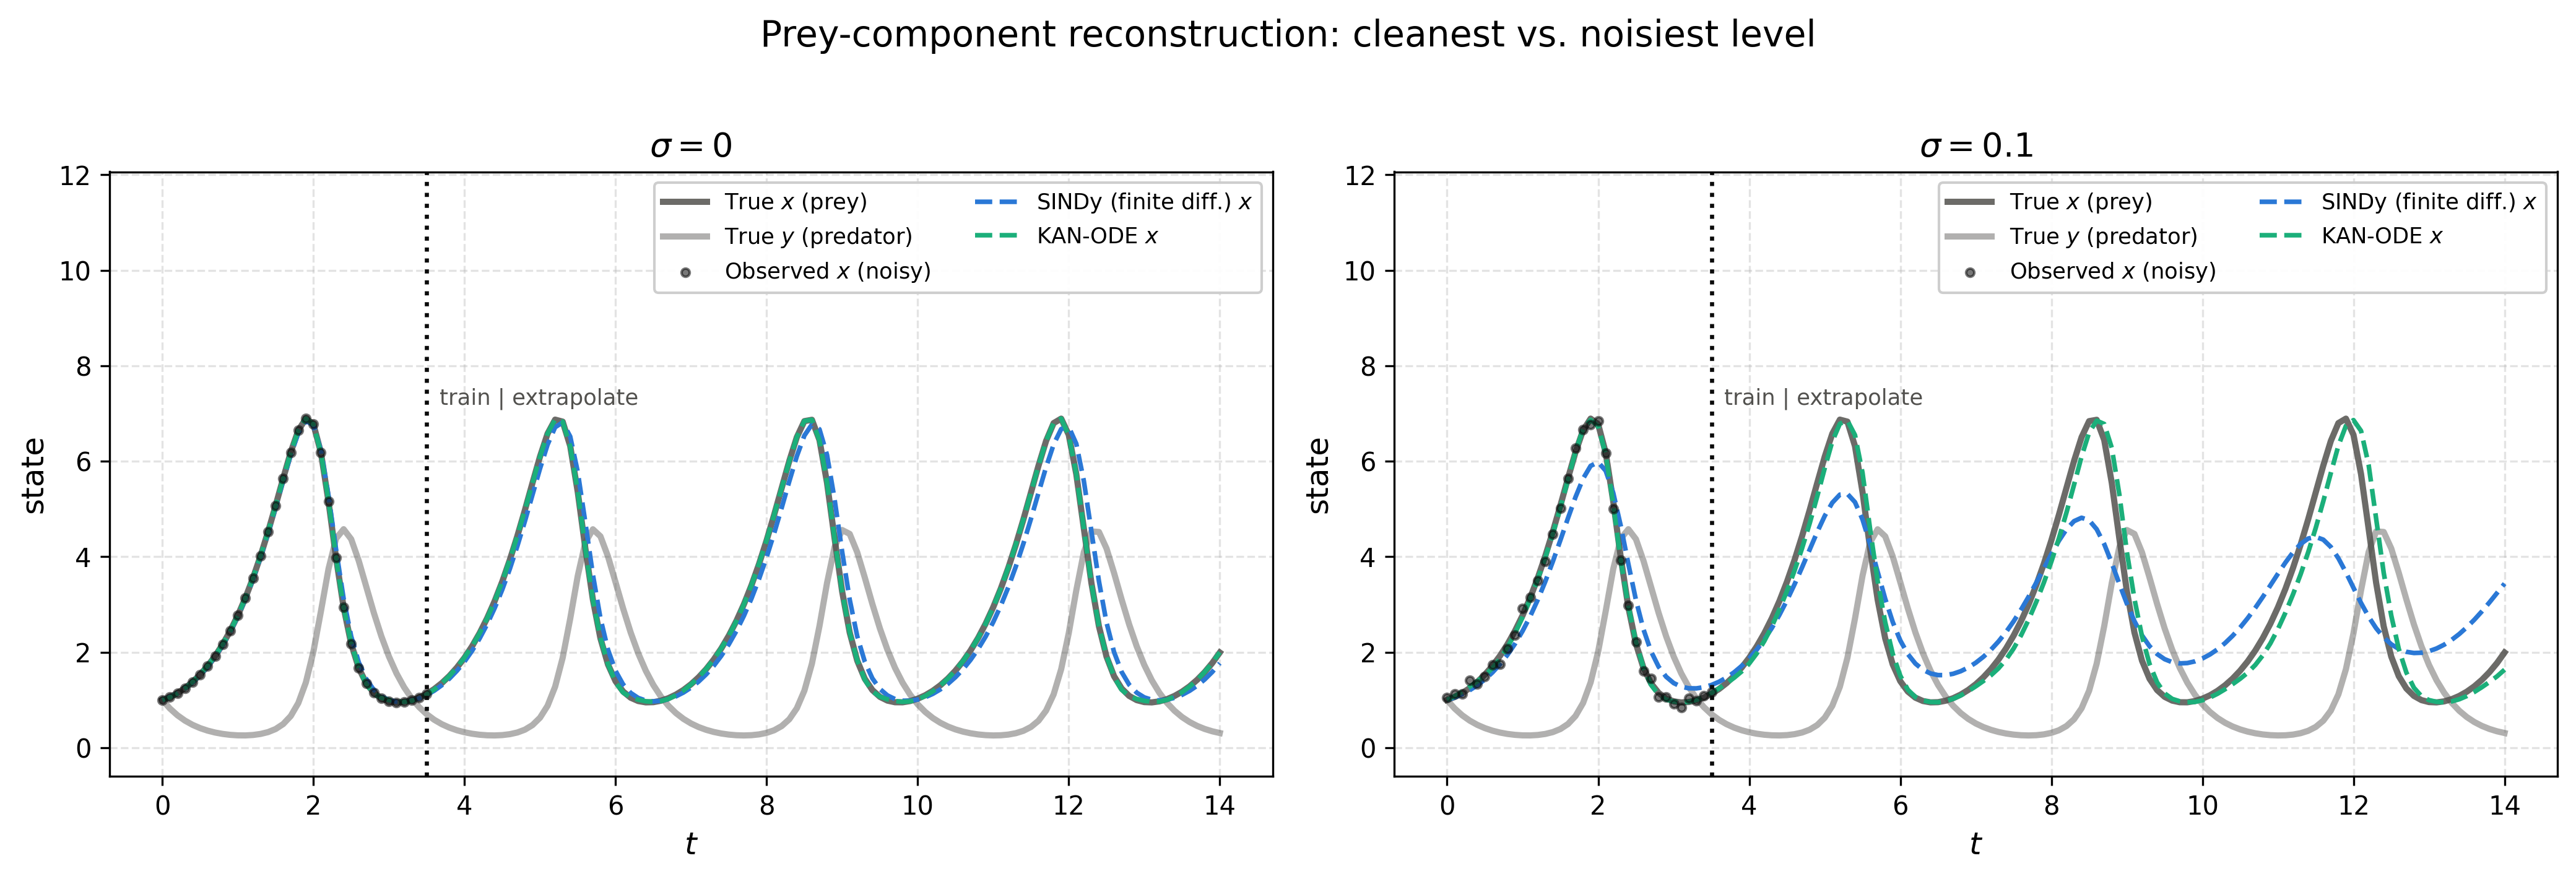
\includegraphics[width=0.85\textwidth]{figures/track_e/sindy_vs_kan_trajectories.png}
\caption{Reconstructed trajectories at $\sigma=0$ and $\sigma=0.1$: sparse
regression loses amplitude under noise; KAN-ODE keeps amplitude but drifts
in phase.}
\label{fig:sindy-trajectories}
\end{figure*}

\subsubsection{Edge pruning: testing whether a term-by-term comparison is even possible}

Part of the original motivation for a smooth, globally-supported basis such
as RBF is that a sparse, pruned KAN edge structure could in principle be read
back as a closed-form symbolic law. Sparse regression reaches the same
interpretability goal by construction. The base paper gets there by adding
the $L_1$ penalty of Equation~\ref{eq:l1-sparsity} to the training loss for
symbolic pruning. Every checkpoint we trained used $\lambda=0$: the plain
mean-squared-error term alone, with no sparsity pressure. A KAN-ODE analogue
of a sparse coefficient list would instead come from pruning weak edges
\emph{post hoc} and reading off what survives. We rank each edge by mean
spline-coefficient magnitude and mask the weakest, applied to the existing
(never retrained) noise-sweep checkpoints. Removing the two weakest of forty
edges raises the noise-free full-horizon MSE from $8.90\times10^{-5}$ to
$3.43$, a factor of $3.9\times10^{4}$ and worse than predicting the constant
dataset mean ($2.91$). No checkpoint was trained with sparsity-inducing
regularization, so nothing during training ever asked the network to
concentrate its fit onto a few edges. The flat plateau at $\approx3.5$--$3.8$
across all pruning levels of 25\% or more is the signature of a model where
every edge carries part of the fit. It confirms that the pruning procedure
itself works correctly on a network that has no prunable structure to find.

\begin{figure*}[t]
\centering
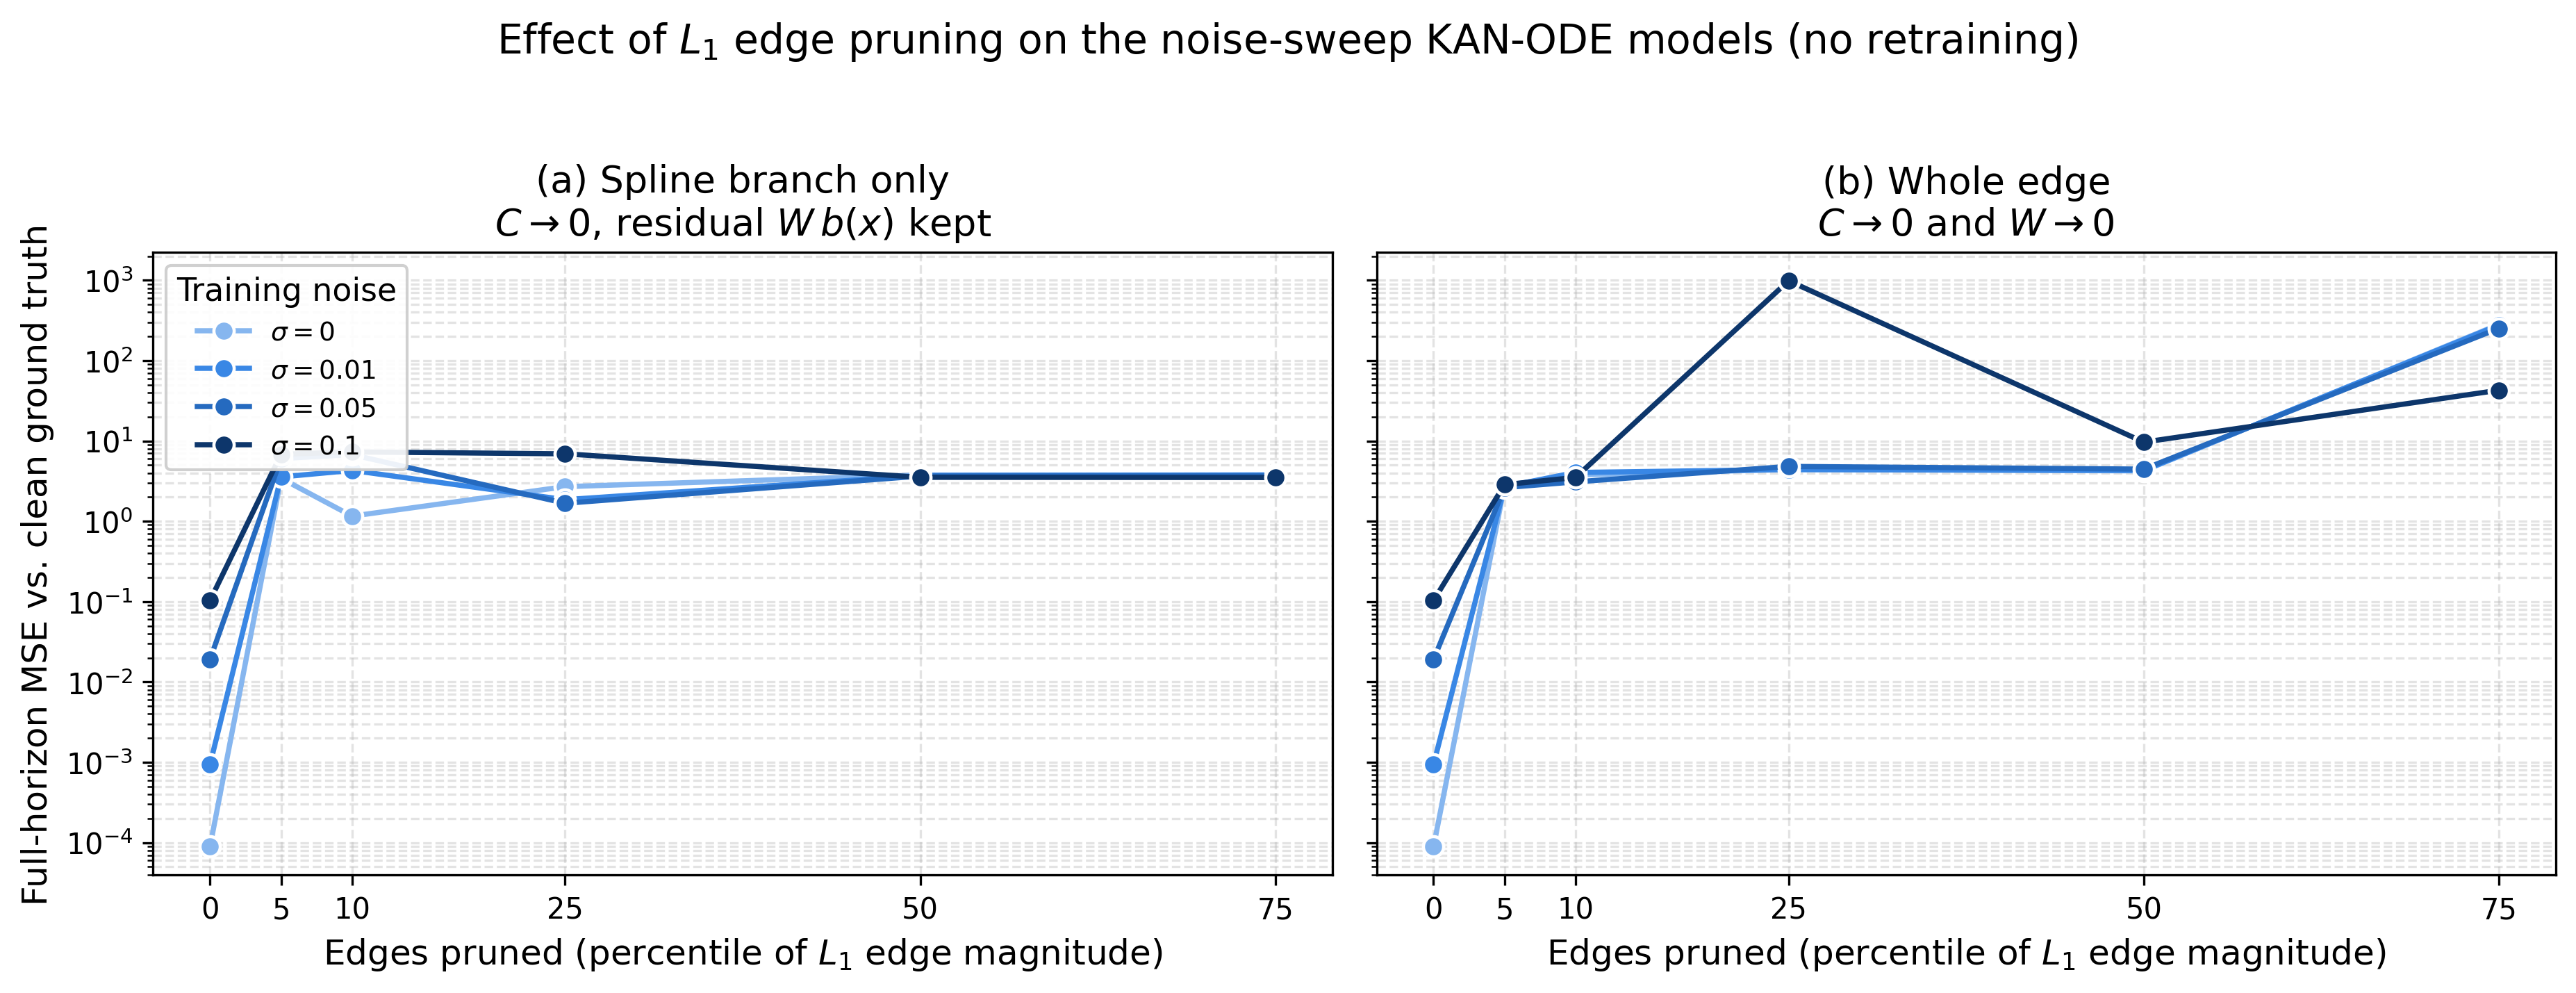
\includegraphics[width=0.85\textwidth]{figures/track_e/pruning_degradation.png}
\caption{Full-horizon MSE vs.\ edge-pruning fraction, all four noise levels.}
\label{fig:pruning}
\end{figure*}

\subsubsection{Testing whether SIR's fixes transfer to a non-mechanistic epidemic curve}

The outbreak curve of Section~\ref{sec:datasets}, which no compartmental ODE
generated, tests whether the SIR fixes of Section~\ref{sec:crossdomain}
generalize by mechanism rather than by coincidence of the SIR system's own
structure. The same init-time diagnostic we used to root-cause SIR
reproduces an almost identical speed-mismatch signature ($18.77\times$ vs.\
SIR's $19\times$). This justifies a time rescaling by a factor of 24
\emph{a priori}, before any training.

\begin{expectbox}
\expectrow{Question}{SIR's three stability fixes were each derived from a property of the SIR generator itself -- do they still work on data no compartmental model produced?}
\expectrow{Expected}{Only the unit-rescaling fix, which assumes nothing about the data's structure, should transfer; the two structural fixes should not.}
\expectrow{Observed}{One in three predictions was wrong: the vanishing-field gate transfers and is the best single option, despite being predicted inapplicable.}
\end{expectbox}

\begin{table*}[t]
\centering
\small
\renewcommand{\arraystretch}{1.15}
\caption{Which of SIR's three fixes transfer to a non-mechanistic curve.}
\label{tab:fix-transfer}
\begin{tabularx}{\textwidth}{@{}L{4.2cm} L{5.0cm} C{3.0cm} Y@{}}
\toprule
\hdrrow \thh{Fix} & \thh{Precondition} & \thh{Holds?} & \thh{Outcome}\\
\midrule
Time rescaling & None -- a unit change & Yes & Removes a $263{,}049\times$ gradient spike\\
Conservation via subspace projection & An exact invariant, $\sum y=c$ & No ($\sum y$ spans $0.002$--$1.54$) & Inapplicable; $25\times$ worse fit\\
Vanishing-field gate at the equilibrium point & $y_d=0$ is a manifold of equilibria & Yes (unexpectedly) & Best single option, $47\times$ better fit\\
\bottomrule
\end{tabularx}
\end{table*}

The vanishing-field gate was \emph{predicted} inapplicable: the infected
fraction at $t=0$ is $0.0027$, which seemed too small to avoid freezing the
field entirely. A control arm overturns that prediction. Gating the learned
field by the initial state correctly encodes that the rate of change is
proportional to current prevalence. It is the only configuration that
reproduces the existence of a peak (day 48 predicted vs.\ true day 45) from a
training window that never observed one.

\begin{figure*}[t]
\centering
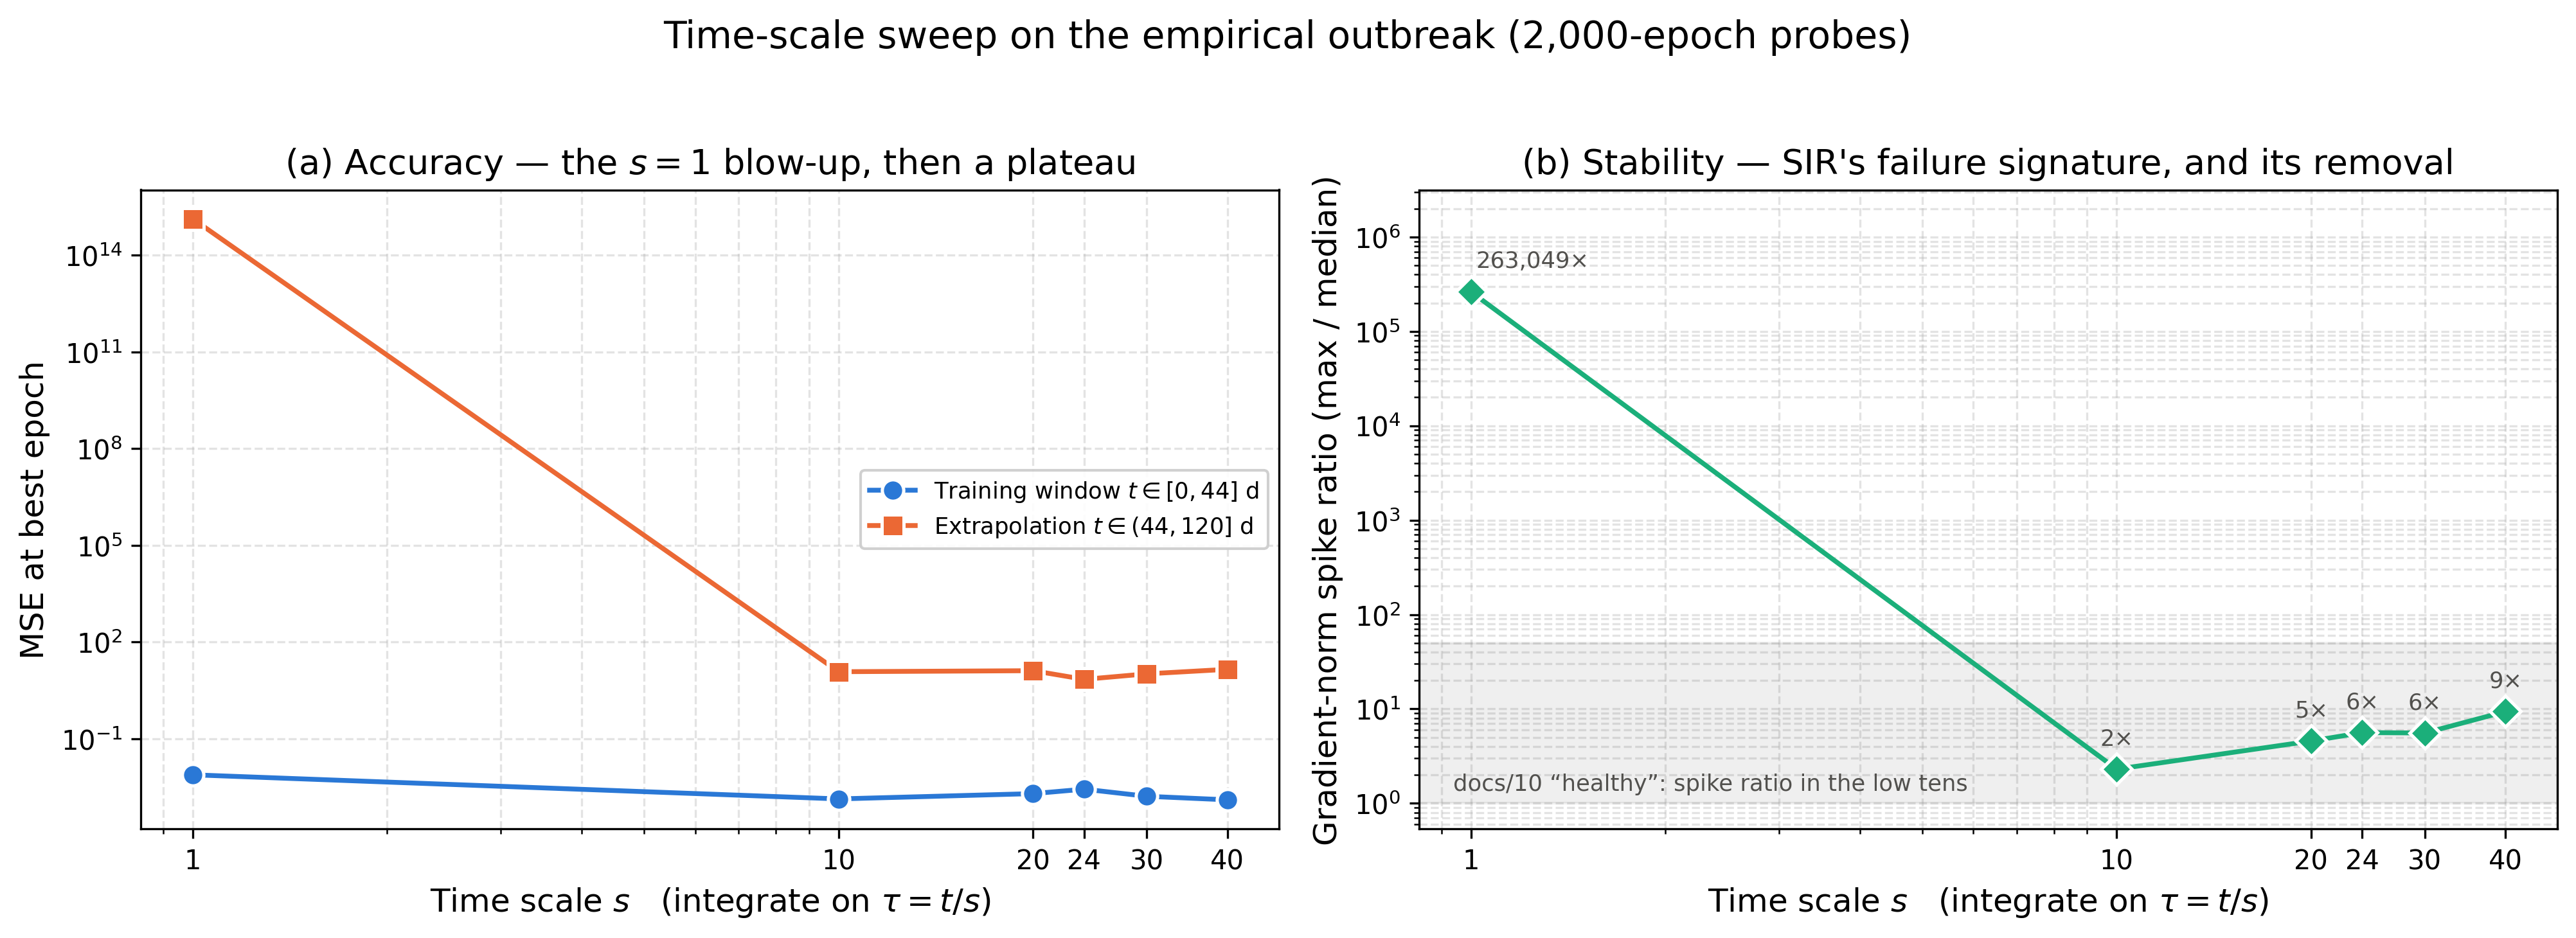
\includegraphics[width=0.85\textwidth]{figures/track_e/epidemic_time_scale_sweep.png}
\caption{Time-rescaling sweep: accuracy and gradient-spike ratio vs.\ the
rescaling factor.}
\label{fig:time-scale-sweep}
\end{figure*}

\paragraph{The extrapolation runaway traces to the train/test split.} The
default split lands exactly on the infected peak (0\% of the decay phase is
in the training window), so every model is asked to predict a monotone decay
it has never observed. Moving the split just 15 days later collapses the
predicted maximum from $6.18\times$ the true peak to $0.964$ (true maximum
$=1.0$), turning over at day 47 against a true day 45. The runaway is a
property of where the window ends, not of the method fitting the data.

\begin{figure*}[t]
\centering
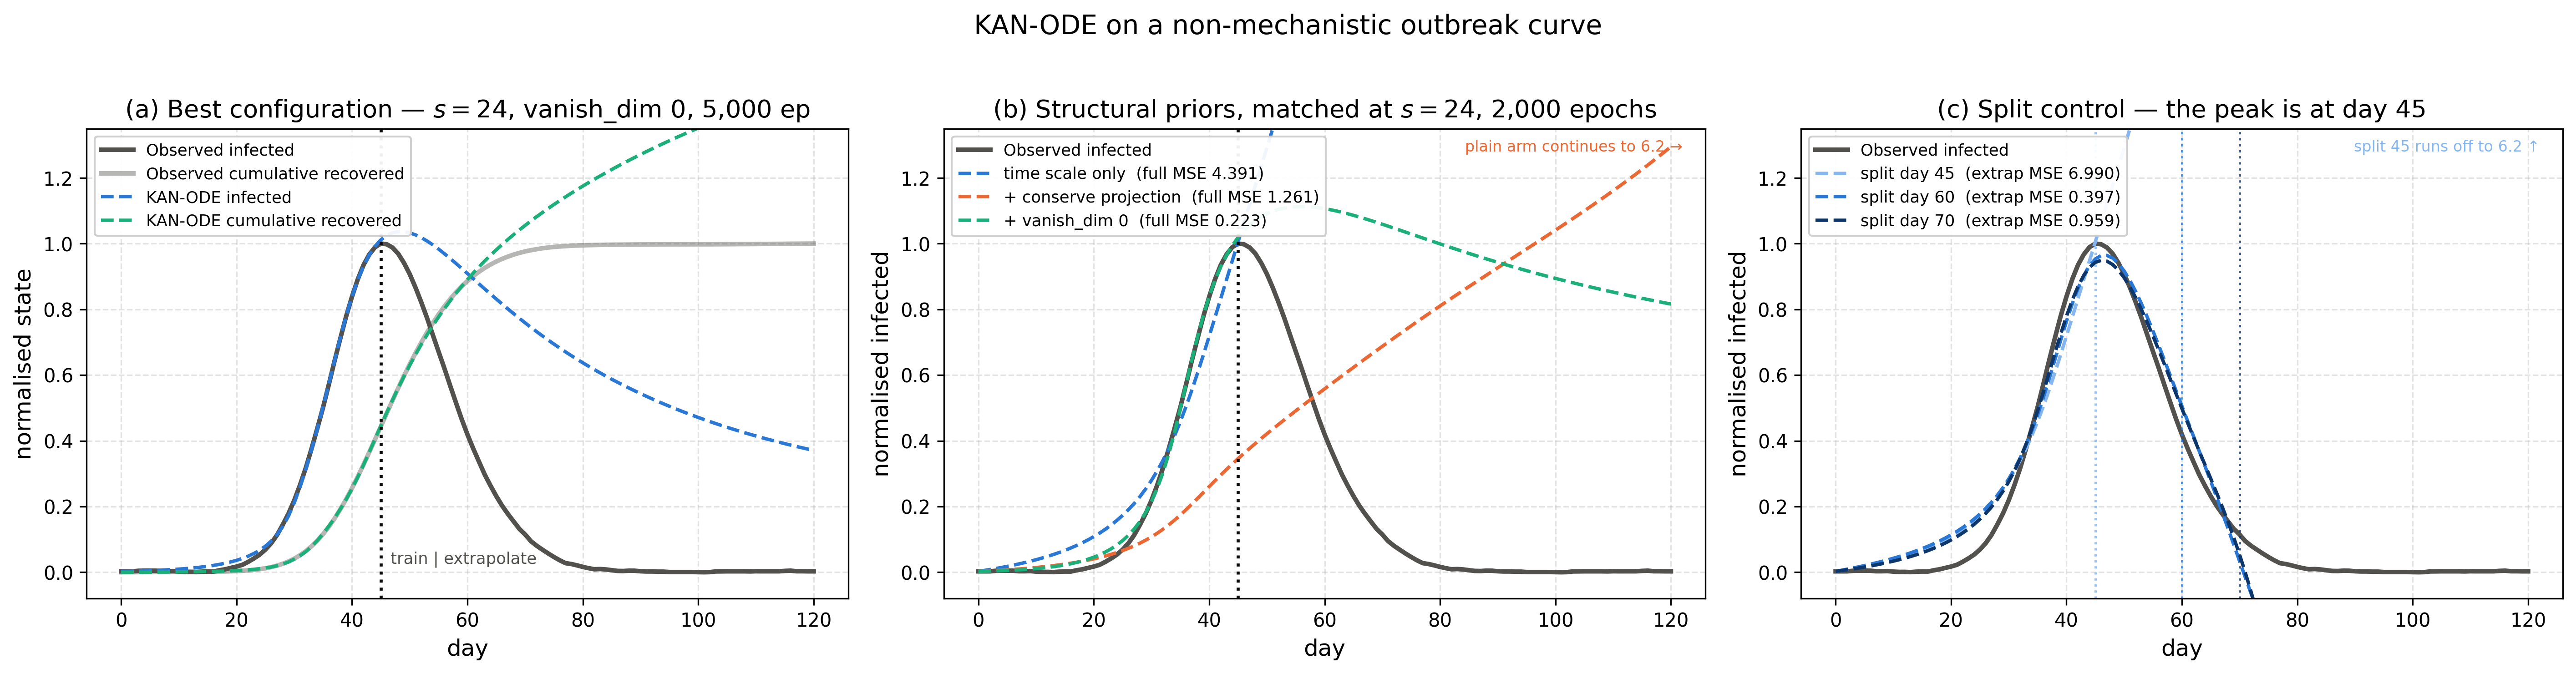
\includegraphics[width=0.85\textwidth]{figures/track_e/real_epidemic_fit.png}
\caption{Epidemic-curve fit: default split (runaway), the vanishing-field-gate
arm, and the fifteen-day-later split control.}
\label{fig:real-epidemic-fit}
\end{figure*}

\begin{keypoint}[Verdict]
Time rescaling transfers unconditionally because it is a unit change with no
structural precondition. The other two fixes are structural priors that
transfer exactly insofar as their structure is actually present in the new
data: the conservation projection's precondition is confirmable in advance
by directly measuring the compartment sum, while the vanishing-field gate's
precondition turned out to require running the control arm to settle --
argument alone predicted the wrong outcome. That arm cost 27 minutes and
overturned the prediction.
\end{keypoint}

\subsection{Epoch-budget validation}
\label{sec:phase4}

Every result in Sections~\ref{sec:kan-vs-mlp}--\ref{sec:track-e} was measured
at a fixed $10^4$-epoch budget, a tenth of the base paper's, for the cost
reasons of Section~\ref{sec:budget}. Here we ask whether that budget is long
enough for the \emph{rankings} to be trusted, and whether any gap to the
paper comes from the budget or from an implementation difference.

\begin{expectbox}
\expectrow{Question}{Do the conclusions drawn at $10^4$ epochs survive five times the training budget?}
\expectrow{Expected}{Absolute errors fall; orderings between configurations hold, since every $10^4$-epoch model had already reached a training loss near $10^{-4}$.}
\expectrow{Observed}{Three of four conclusions hold. The fourth, the one the paper headlines, reverses: at $5\times10^4$ epochs the parameter-matched MLP extrapolates $6.8\times$ \emph{better} than KAN-ODE.}
\end{expectbox}

\subsubsection{Design}

We chose five configurations to test the conclusions most exposed to the
budget: Euler (the one solver short of $10^{-4}$ at $10^4$ epochs),
Tsit5/RBF (the reference), B-spline (the near-tie with RBF), and both MLP
baselines. Each was retrained from scratch at $5\times10^4$ epochs with the
recipe of Table~\ref{tab:recipe} unchanged, on cloud CPUs. The B-spline run
was cut to $2.5\times10^4$ epochs because its short calibration run
predicted about 35 hours for the full budget. The real run turned out
$1.63\times$ faster than that calibration ($1.544$ against $2.52$~s/epoch),
a reminder that a five-epoch sample is dominated by start-up cost. The batch
used $23.2$ serial CPU-hours against a planned $17.0$, and $10.7$ hours of
wall-clock with the five jobs in parallel. Before analysis we checked every
run's stored metrics against the epoch count of its training log, and
reloaded and re-scored every checkpoint; the rollouts reproduce the stored
extrapolation MSE to within $0.6\%$.

We added a sixth configuration later, as a separate follow-up. The
implementation audit (Section~\ref{sec:audit}) turned up the base paper's own
learning rate and initialization scale for its MLP baseline, so we reran
both budgets with the identical $[2,50,2]$ tanh architecture under those
settings instead of our default. We report it alongside the original five
throughout.

\subsubsection{Results}

\begin{table*}[t]
\centering
\footnotesize
\renewcommand{\arraystretch}{1.1}
\caption{The five originally planned configurations at $10^4$ epochs
(Sections~\ref{sec:kan-vs-mlp}--\ref{sec:basis-results}) and at the extended budget, plus a sixth added
after auditing the paper's own optimizer settings for its MLP baseline
(Section~\ref{sec:audit}). ``Clip'' is the fraction of optimizer steps on
which gradient clipping at norm $1.0$ engaged; $\|\nabla\|_{\text{med}}$ is
the median pre-clip gradient norm over the extended run. The sixth
configuration ran with no clipping by design (see the paragraph following
this table), so those two columns are blank throughout.}
\label{tab:phase4}
\begin{tabularx}{\textwidth}{@{}Y C{1.1cm} C{2.0cm} C{2.0cm} C{1.8cm} C{1.0cm} C{1.1cm} C{1.6cm}@{}}
\toprule
\hdrrow \thh{Configuration} & \thh{Epochs} & \thh{Training MSE} & \thh{Extrap.\ MSE} & \thh{Extrap.\ $R^2$} & \thh{$\hat L$} & \thh{Clip} & \thh{$\|\nabla\|_{\text{med}}$}\\
\midrule
Euler / RBF & 10k & $1.38\times10^{-4}$ & $2.51\times10^{-3}$ & $0.99914$ & $8.55$ & & \\
 & \textbf{50k} & $8.85\times10^{-6}$ & $1.93\times10^{-4}$ & $0.99993$ & $7.72$ & $4.7\%$ & $0.147$\\
\addlinespace
Tsit5 / RBF & 10k & $8.83\times10^{-5}$ & $8.92\times10^{-5}$ & $0.99997$ & $6.91$ & & \\
 & \textbf{50k} & $6.59\times10^{-6}$ & $4.02\times10^{-5}$ & $0.999986$ & $7.75$ & $4.3\%$ & $0.169$\\
\addlinespace
Tsit5 / B-spline & 10k & $7.20\times10^{-5}$ & $8.38\times10^{-5}$ & $0.99997$ & $8.44$ & & \\
 & \textbf{25k} & $9.65\times10^{-6}$ & $4.26\times10^{-5}$ & $0.999985$ & $7.05$ & $2.2\%$ & $0.033$\\
\addlinespace
MLP-ODE, SiLU & 10k & $9.50\times10^{-5}$ & $4.77\times10^{-4}$ & $0.99984$ & $5.07$ & & \\
 & \textbf{50k} & $\mathbf{1.82\times10^{-6}}$ & $\mathbf{5.90\times10^{-6}}$ & $\mathbf{0.999998}$ & $5.65$ & $11.1\%$ & $0.162$\\
\addlinespace
MLP-ODE, tanh (paper, default lr/init) & 10k & $1.08\times10^{0}$ & $1.69\times10^{0}$ & $0.4215$ & $38.2$ & & \\
 & \textbf{50k} & $1.01\times10^{0}$ & $4.32\times10^{0}$ & $-0.4841$ & $104.8$ & $99.3\%$ & $19.8$\\
\addlinespace
MLP-ODE, tanh (paper's own lr/init) & 10k & $1.11\times10^{-3}$ & $9.65\times10^{-3}$ & $0.99669$ & $9.23$ & & \\
 & \textbf{50k} & $5.43\times10^{-5}$ & $4.31\times10^{-4}$ & $0.99985$ & $9.67$ & -- & -- \\
\bottomrule
\end{tabularx}
\end{table*}

\begin{figure*}[t]
\centering
\begin{subfigure}[b]{0.32\textwidth}
  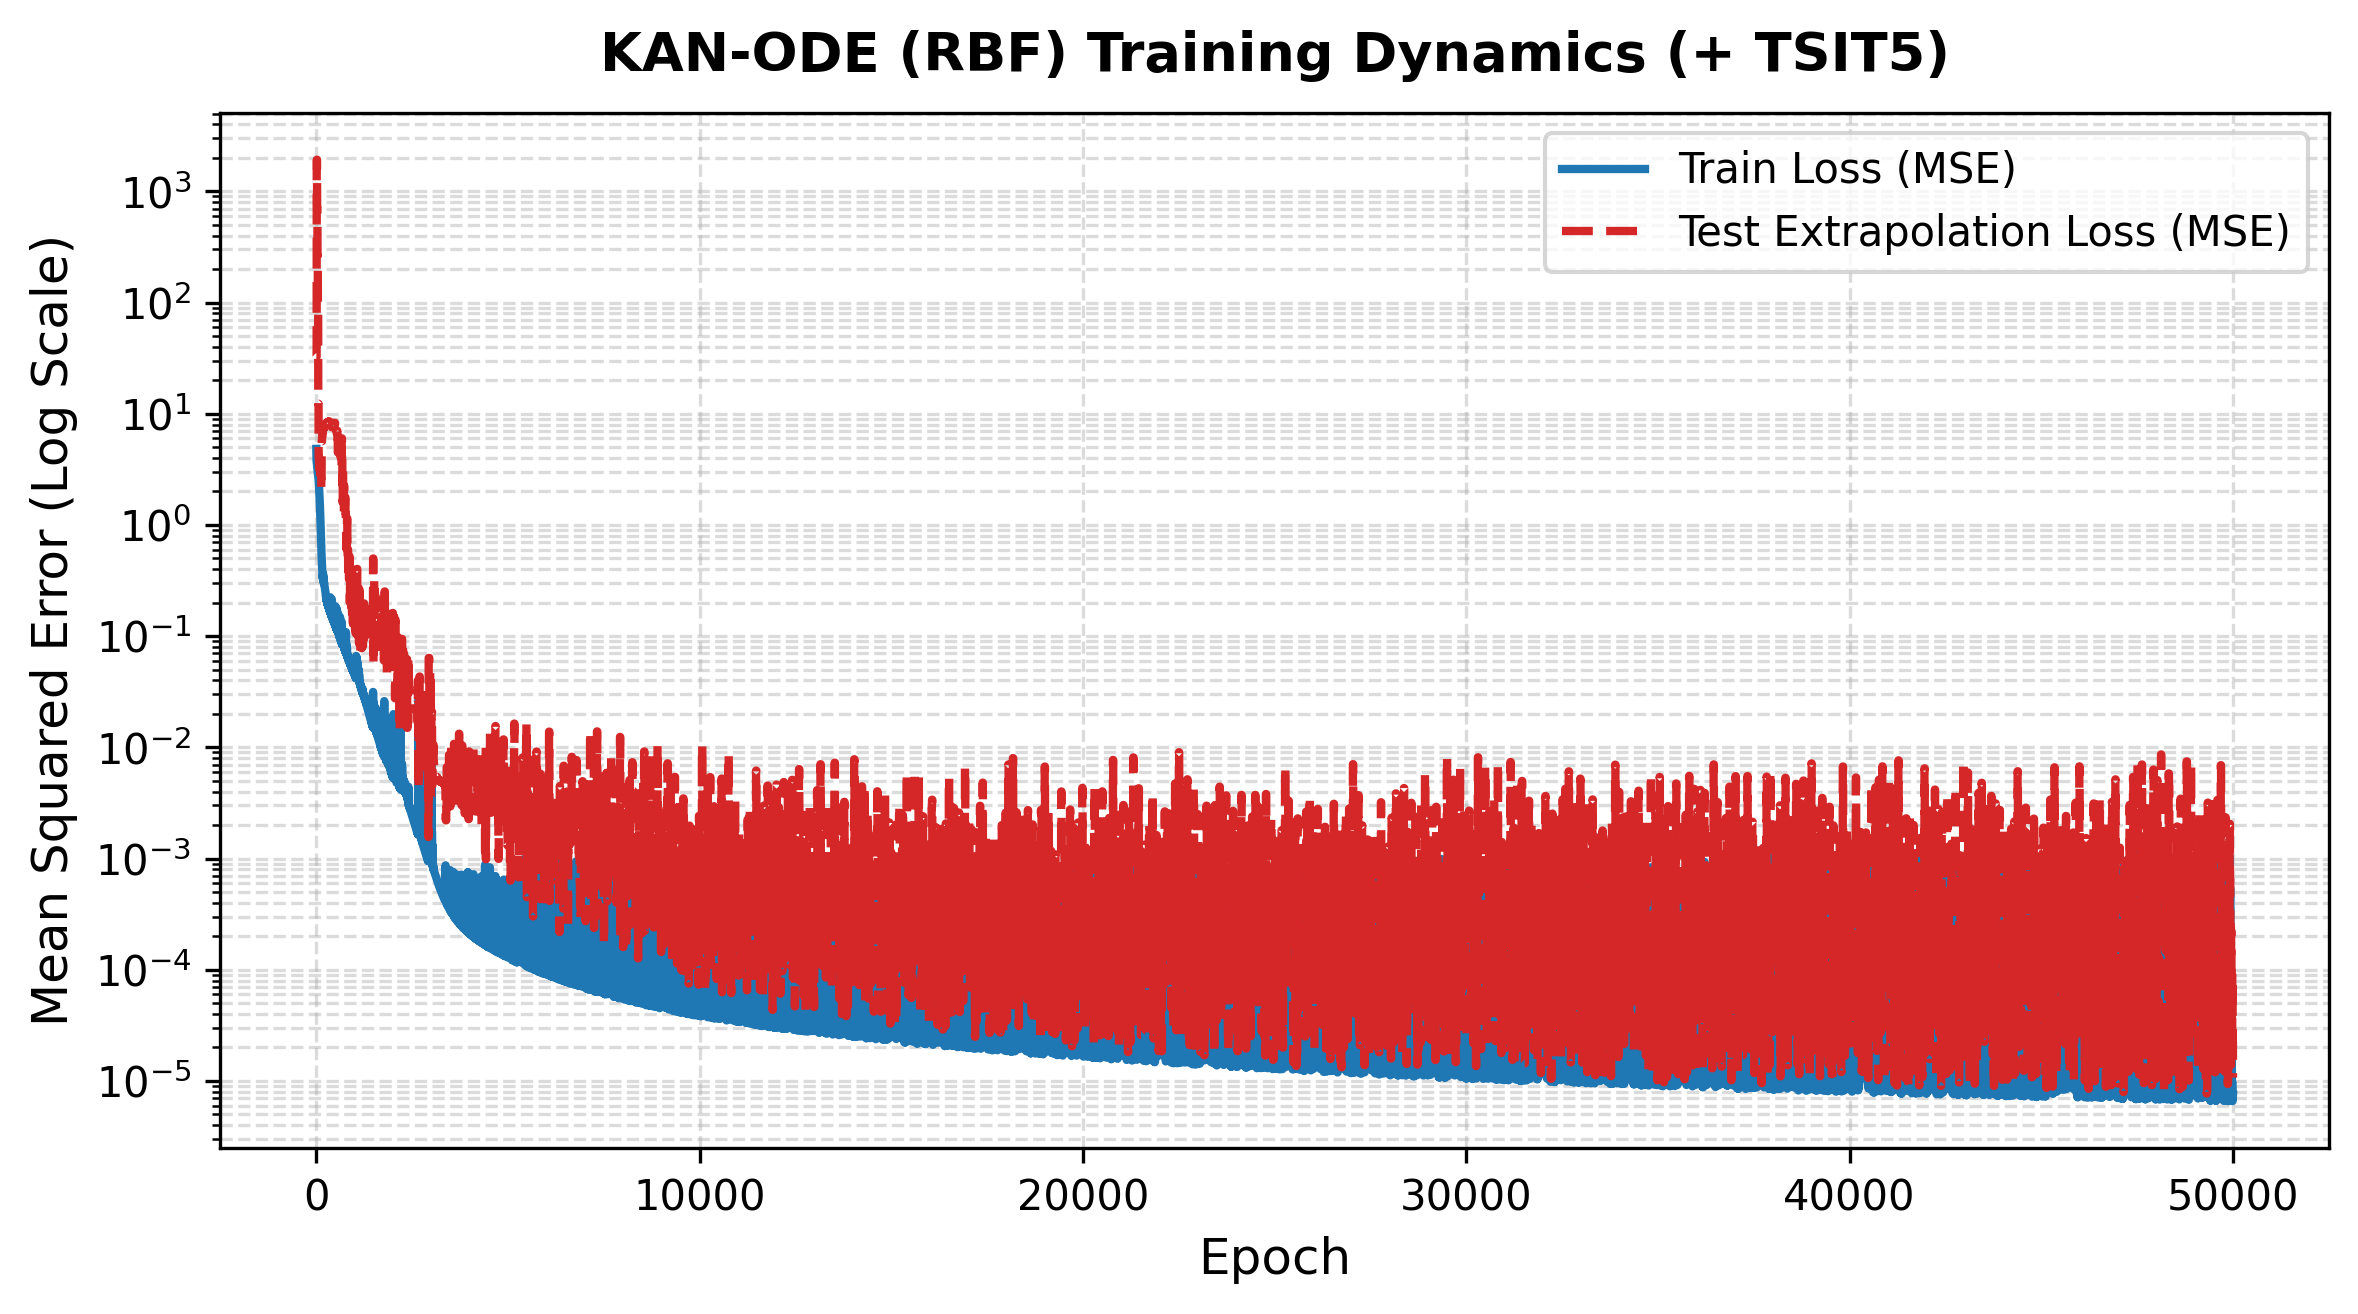
\includegraphics[width=\linewidth]{figures/phase4/tsit5_rbf_50k_loss_curves.png}
  \caption{KAN-ODE, Tsit5 / RBF, 50k}
\end{subfigure}\hfill
\begin{subfigure}[b]{0.32\textwidth}
  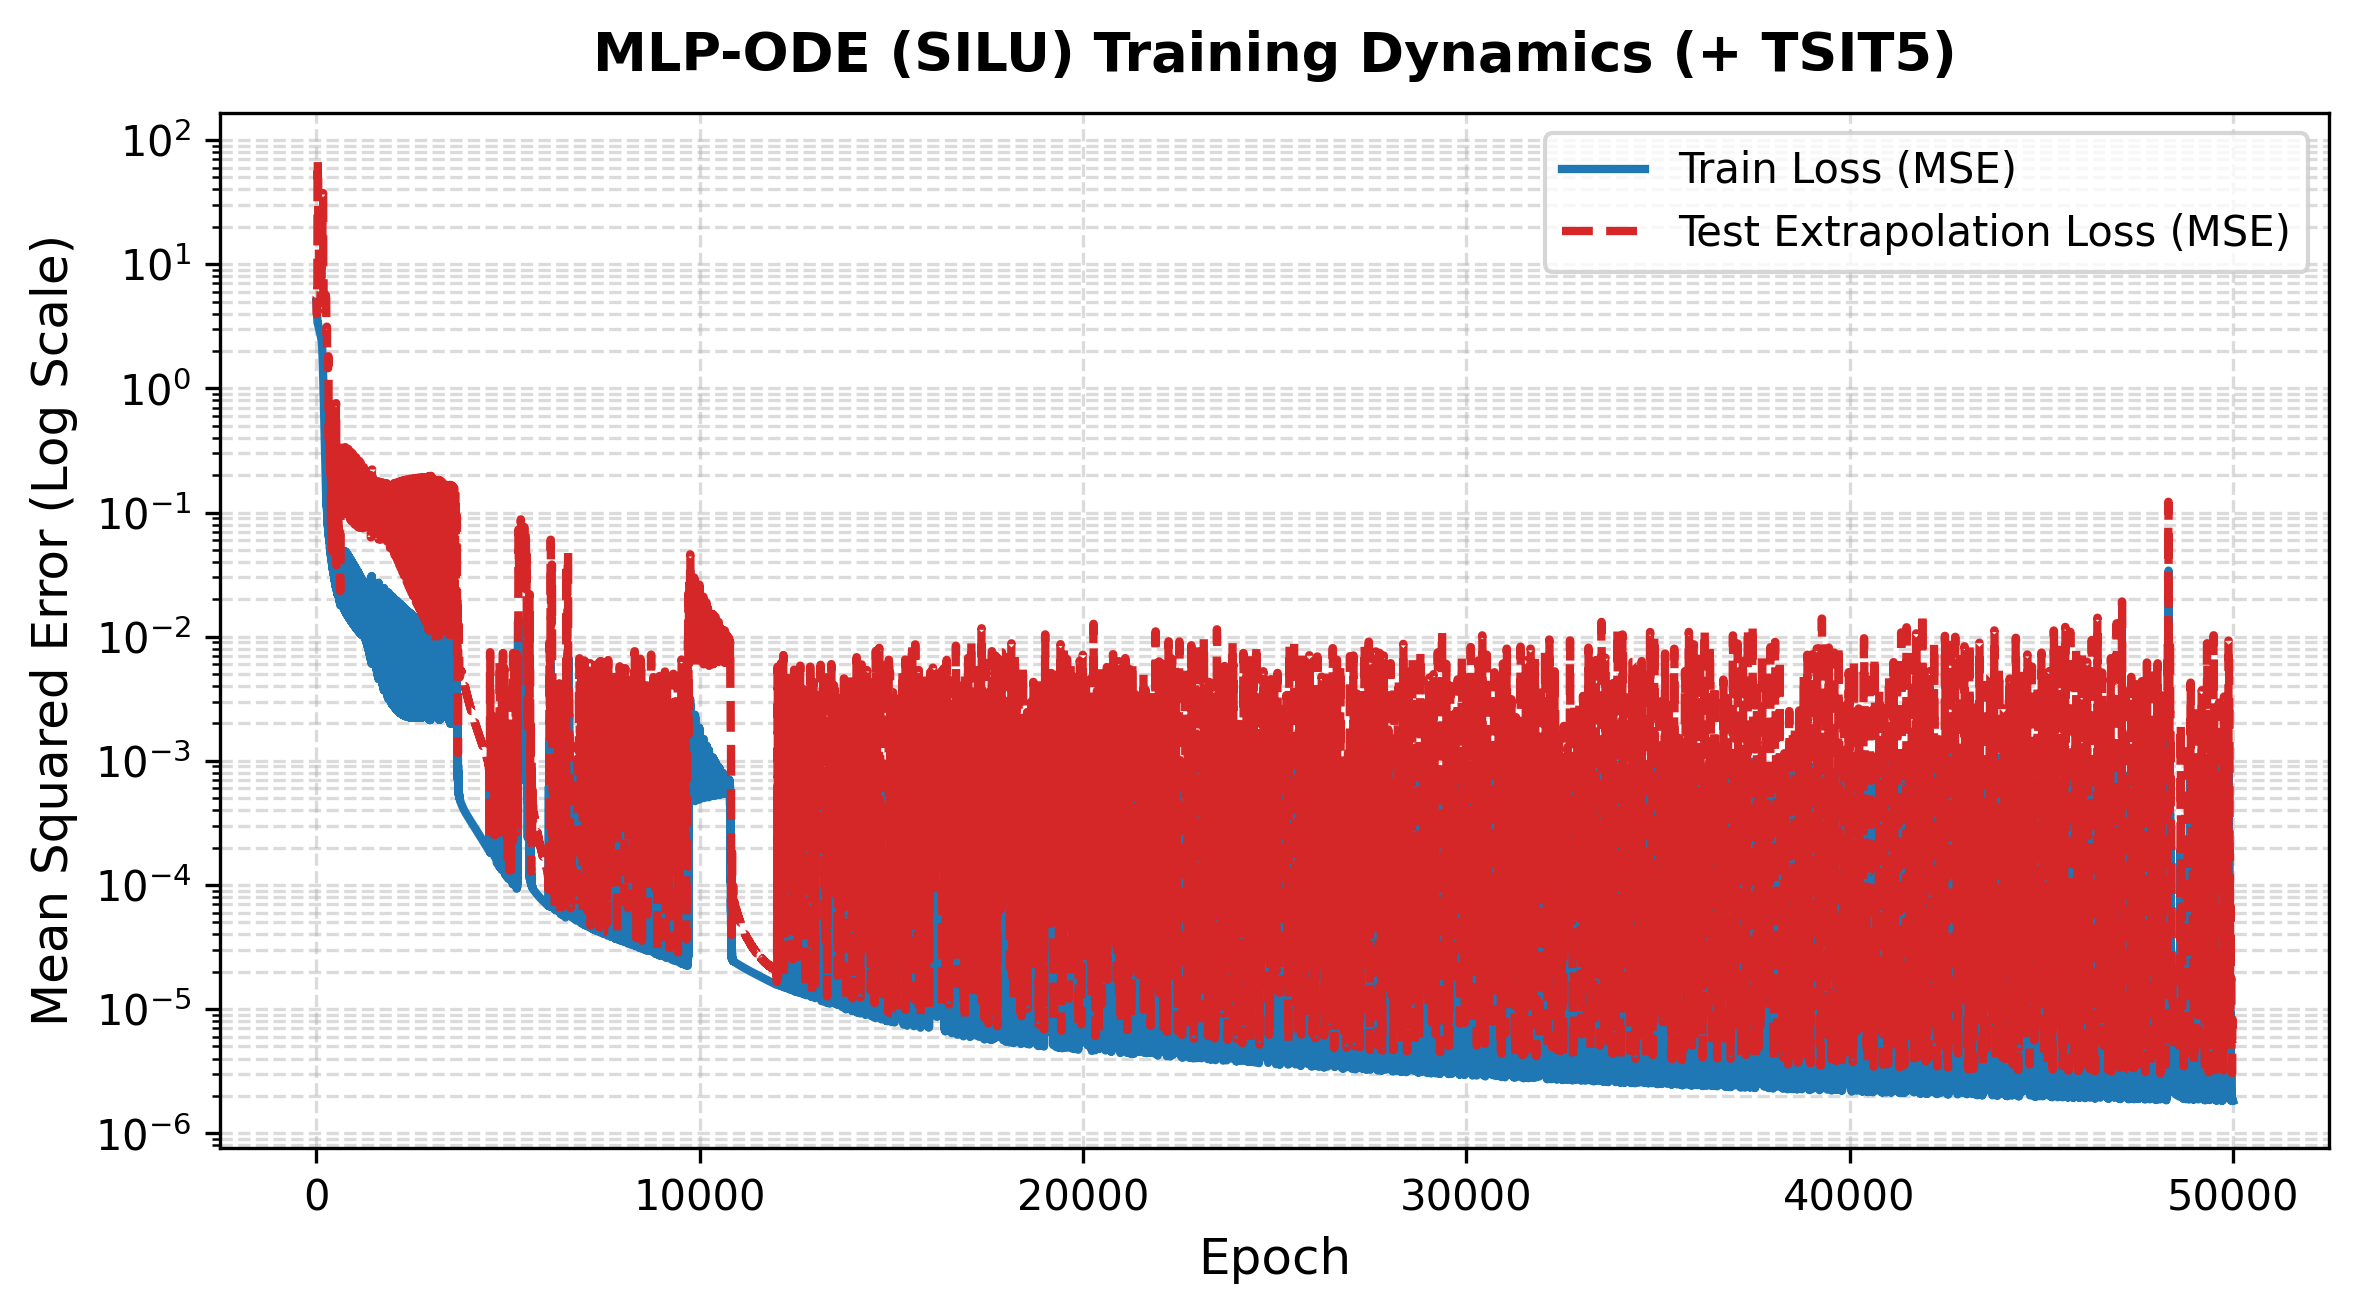
\includegraphics[width=\linewidth]{figures/phase4/mlp_silu_50k_loss_curves.png}
  \caption{MLP-ODE, SiLU, 50k}
\end{subfigure}\hfill
\begin{subfigure}[b]{0.32\textwidth}
  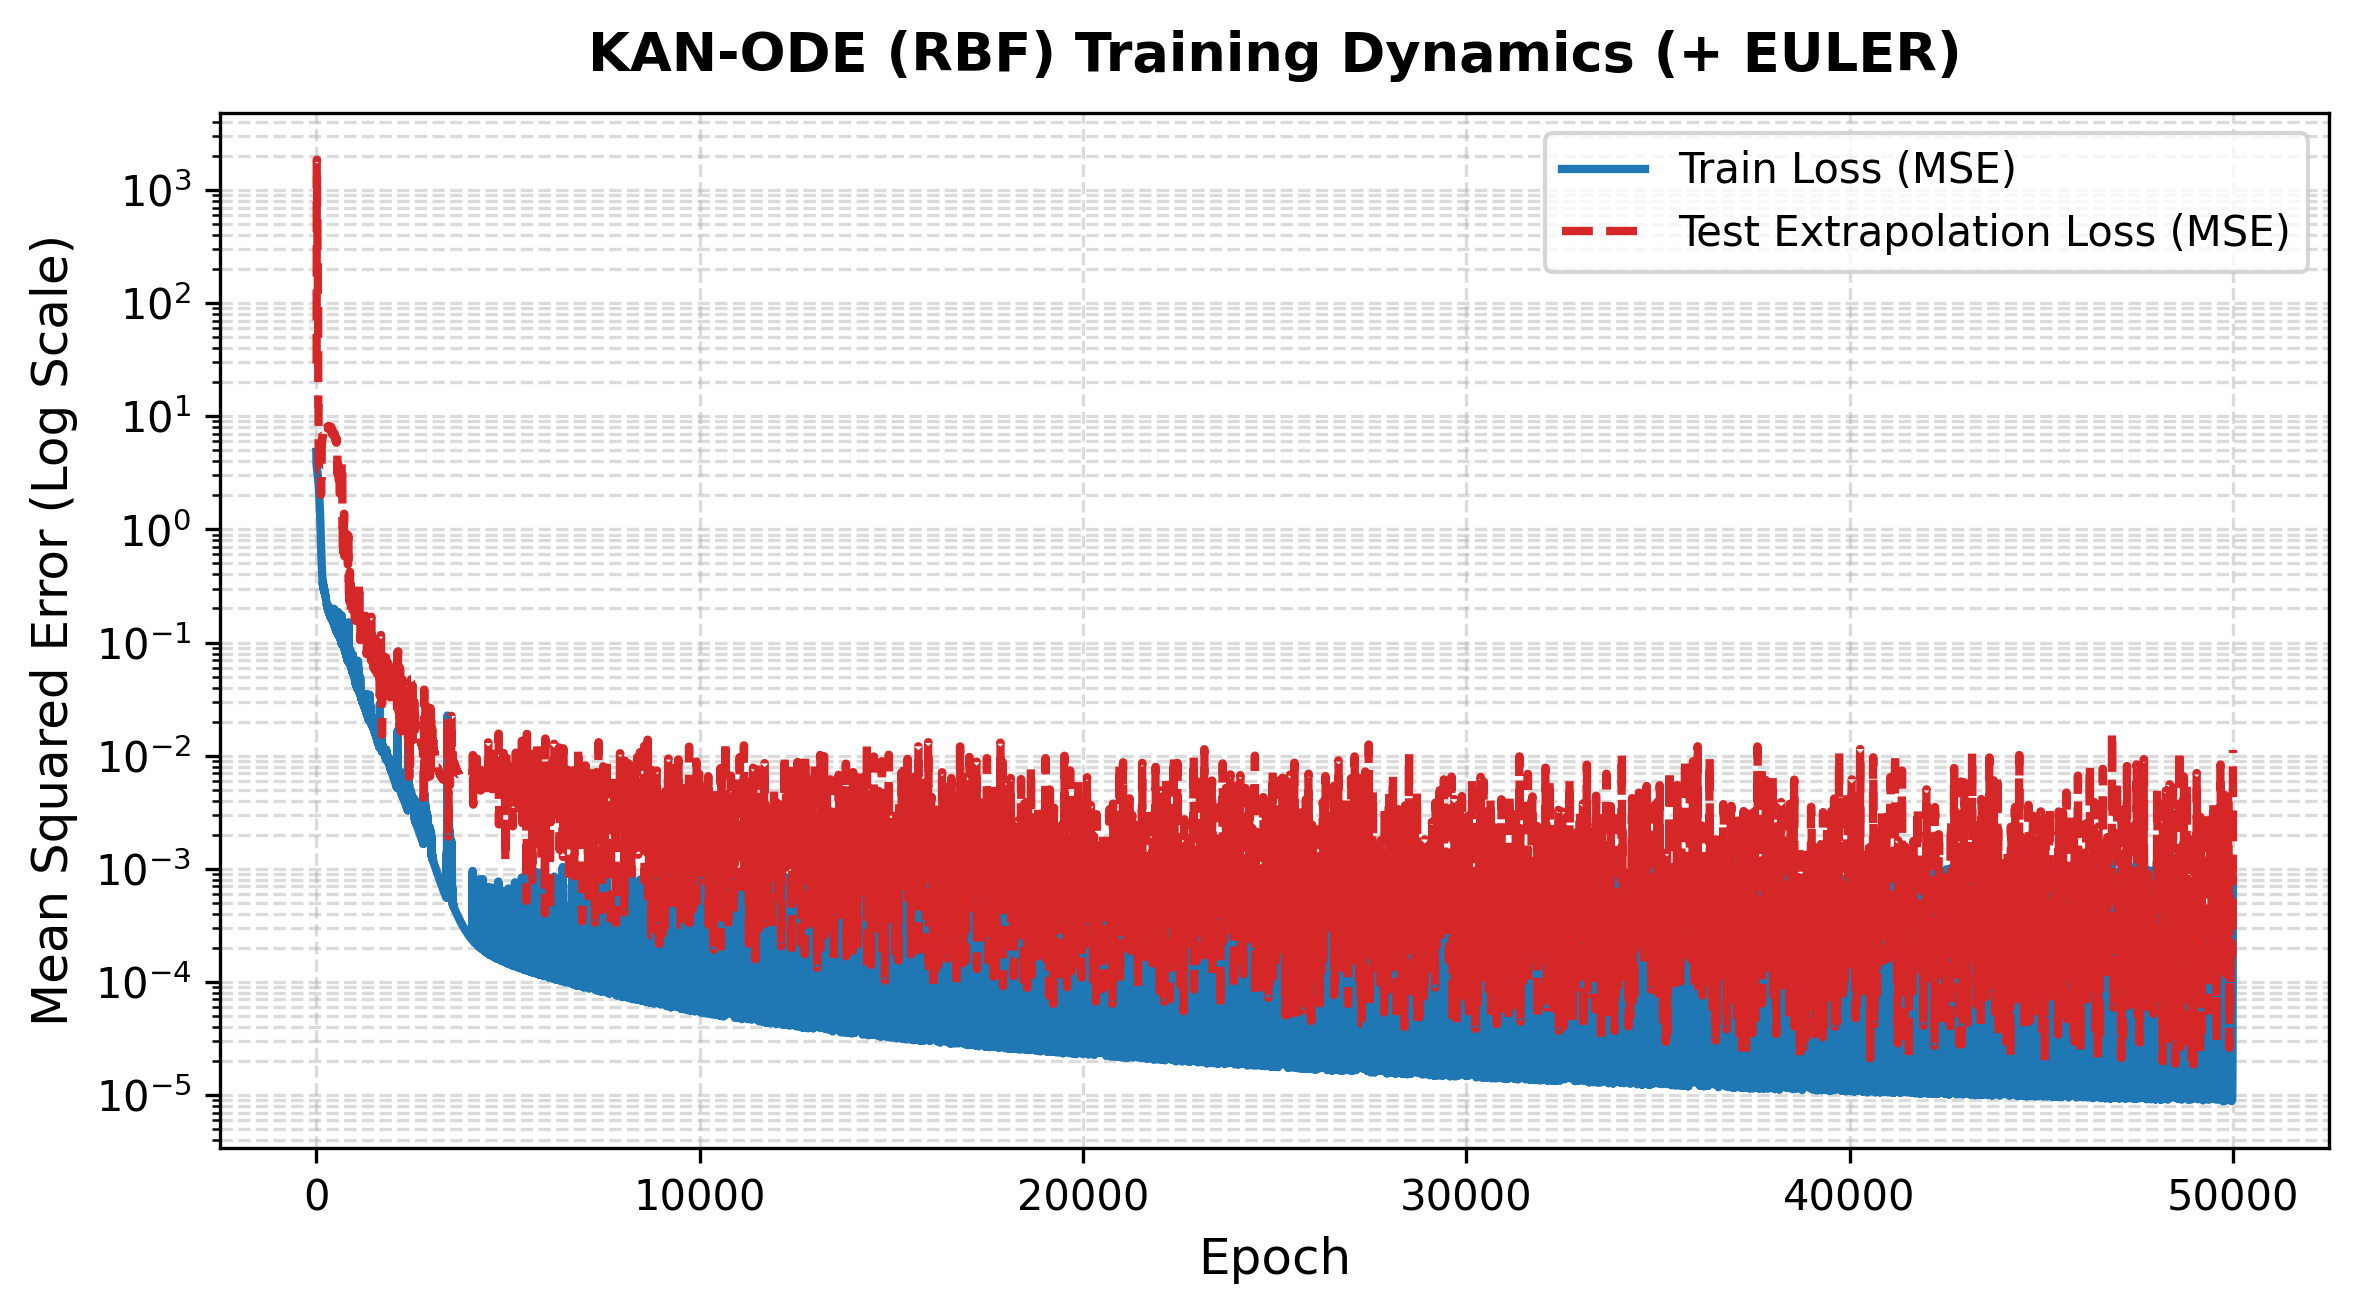
\includegraphics[width=\linewidth]{figures/phase4/euler_50k_loss_curves.png}
  \caption{KAN-ODE, Euler / RBF, 50k}
\end{subfigure}\\[4pt]
\begin{subfigure}[b]{0.32\textwidth}
  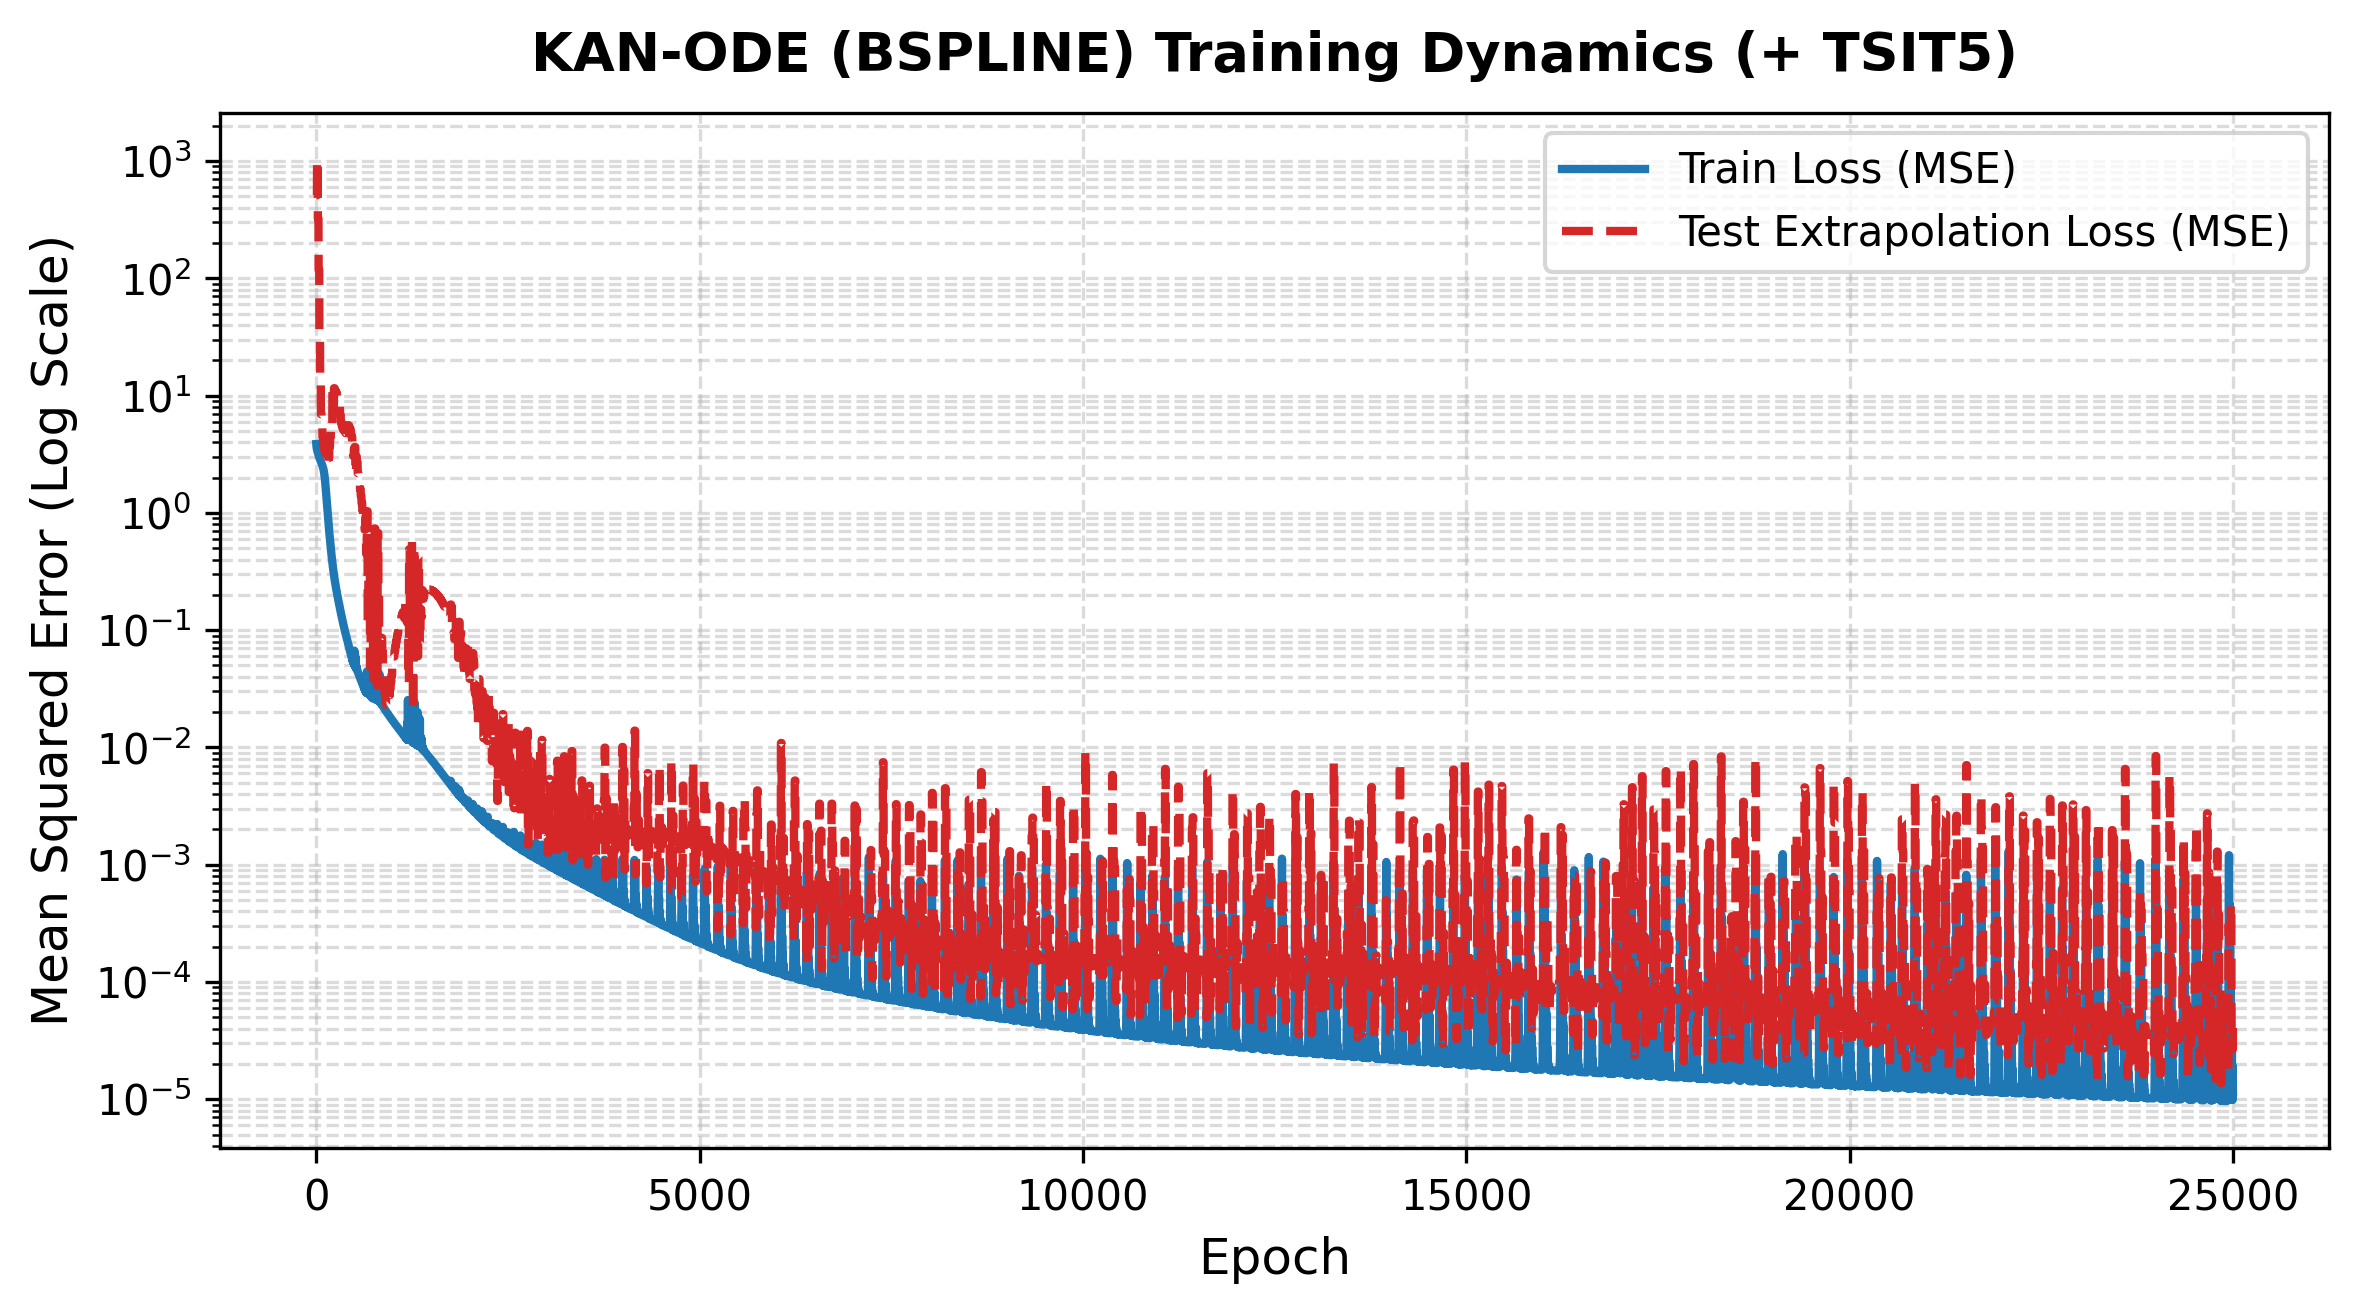
\includegraphics[width=\linewidth]{figures/phase4/bspline_25k_loss_curves.png}
  \caption{KAN-ODE, Tsit5 / B-spline, 25k}
\end{subfigure}\hfill
\begin{subfigure}[b]{0.32\textwidth}
  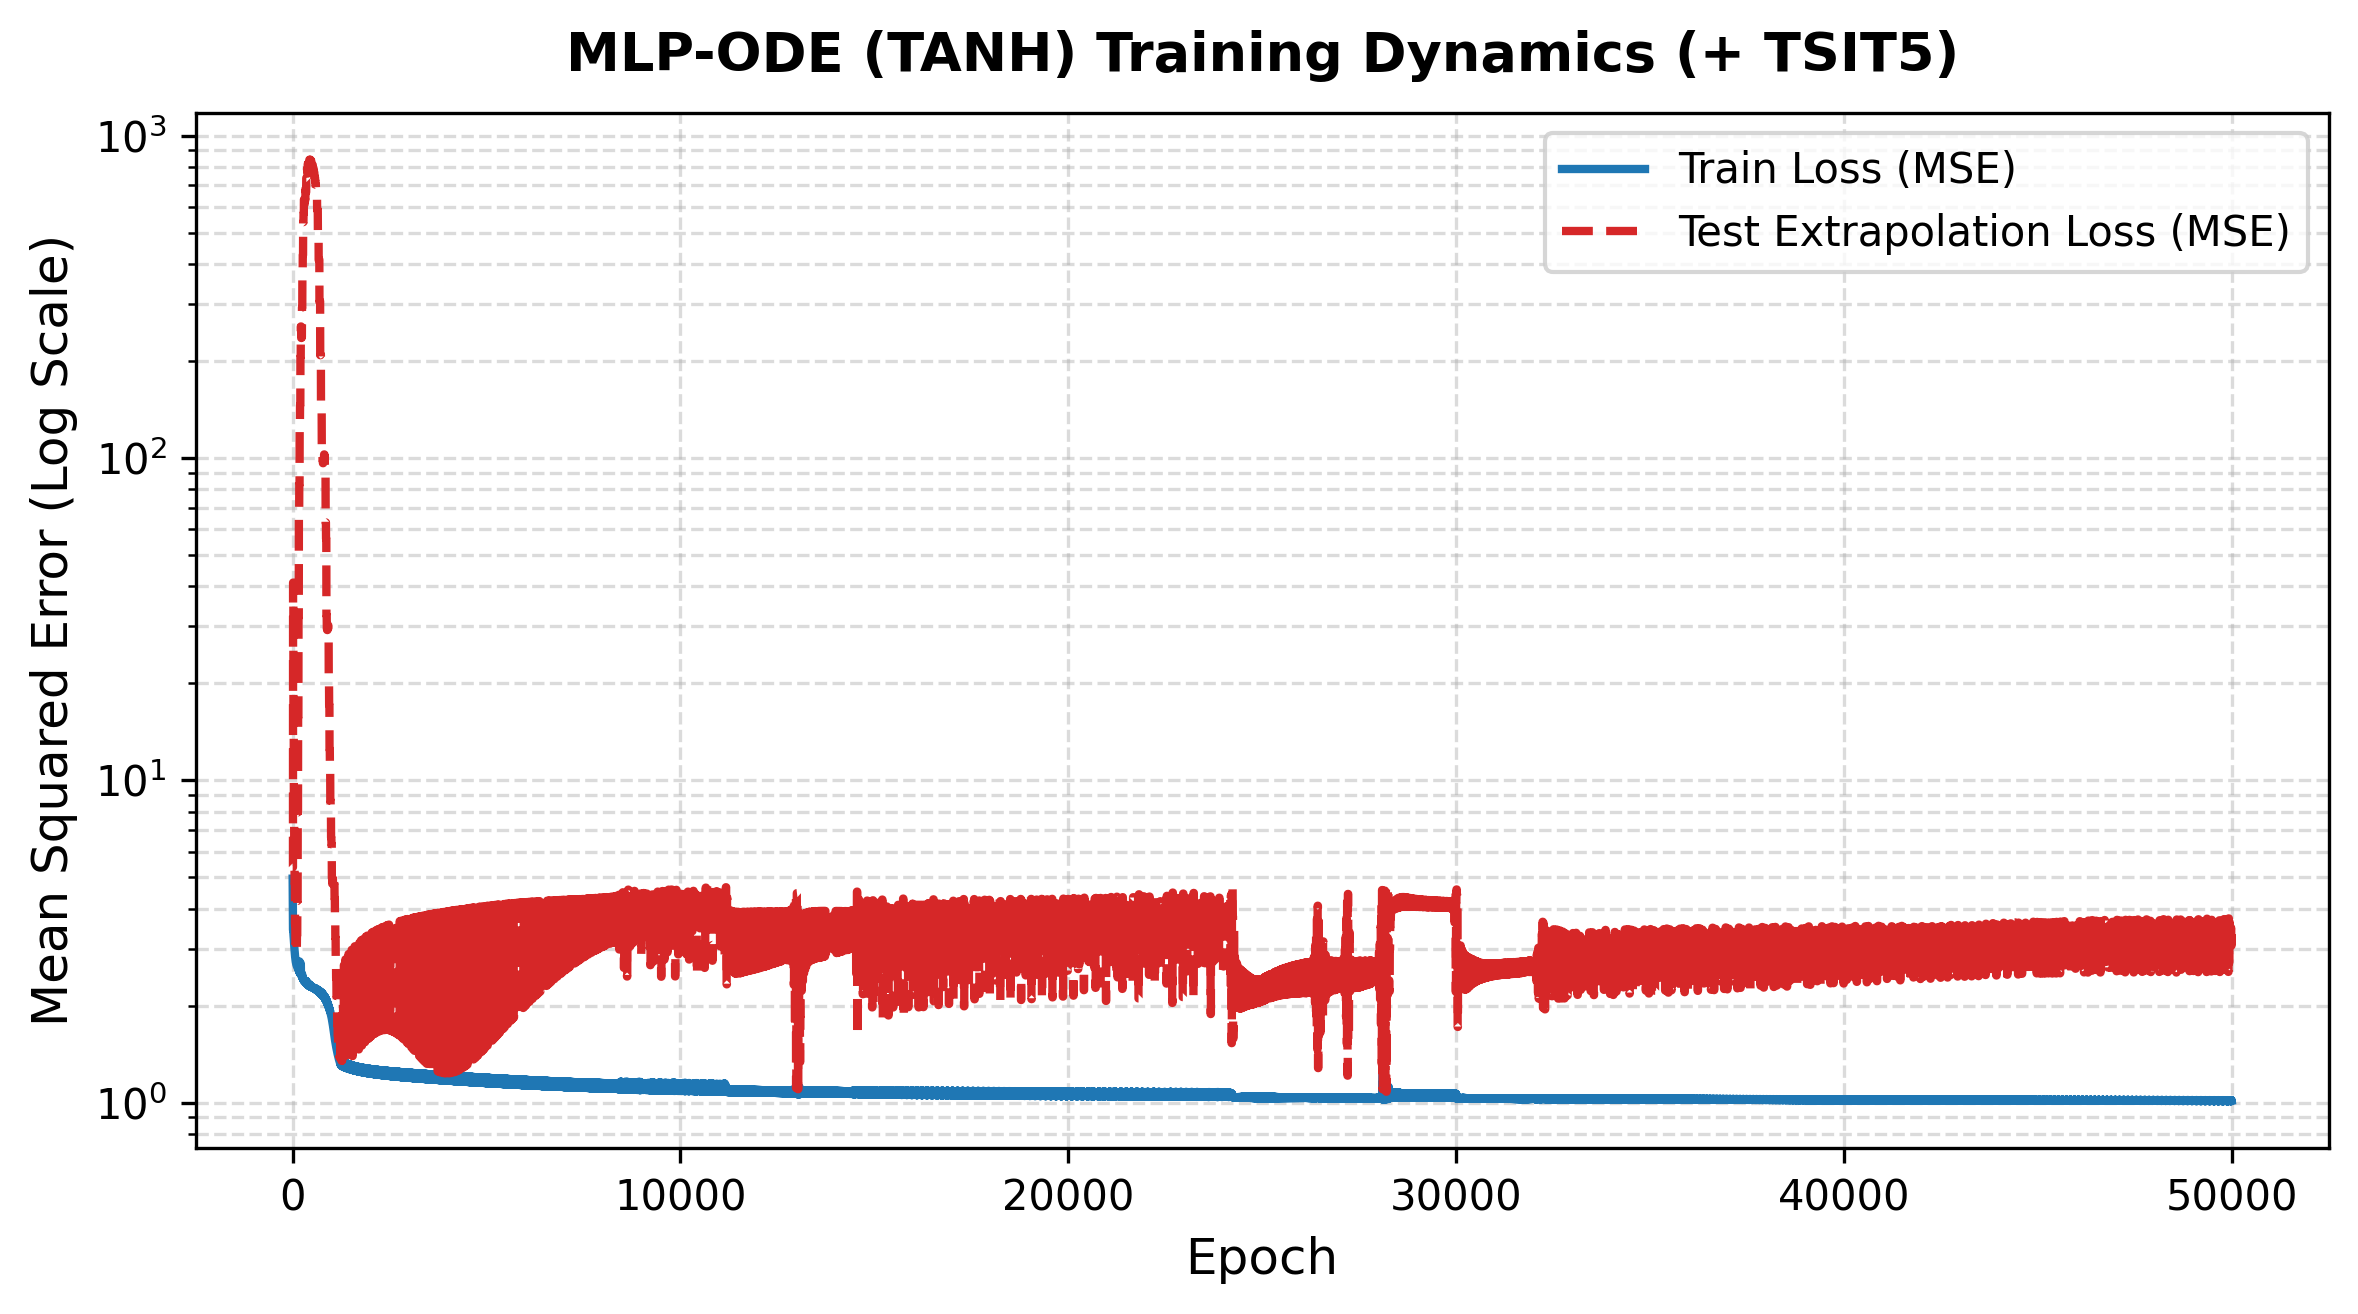
\includegraphics[width=\linewidth]{figures/phase4/mlp_paperspec_50k_loss_curves.png}
  \caption{MLP-ODE, tanh (paper's default lr/init), 50k}
\end{subfigure}\hfill
\begin{subfigure}[b]{0.32\textwidth}
  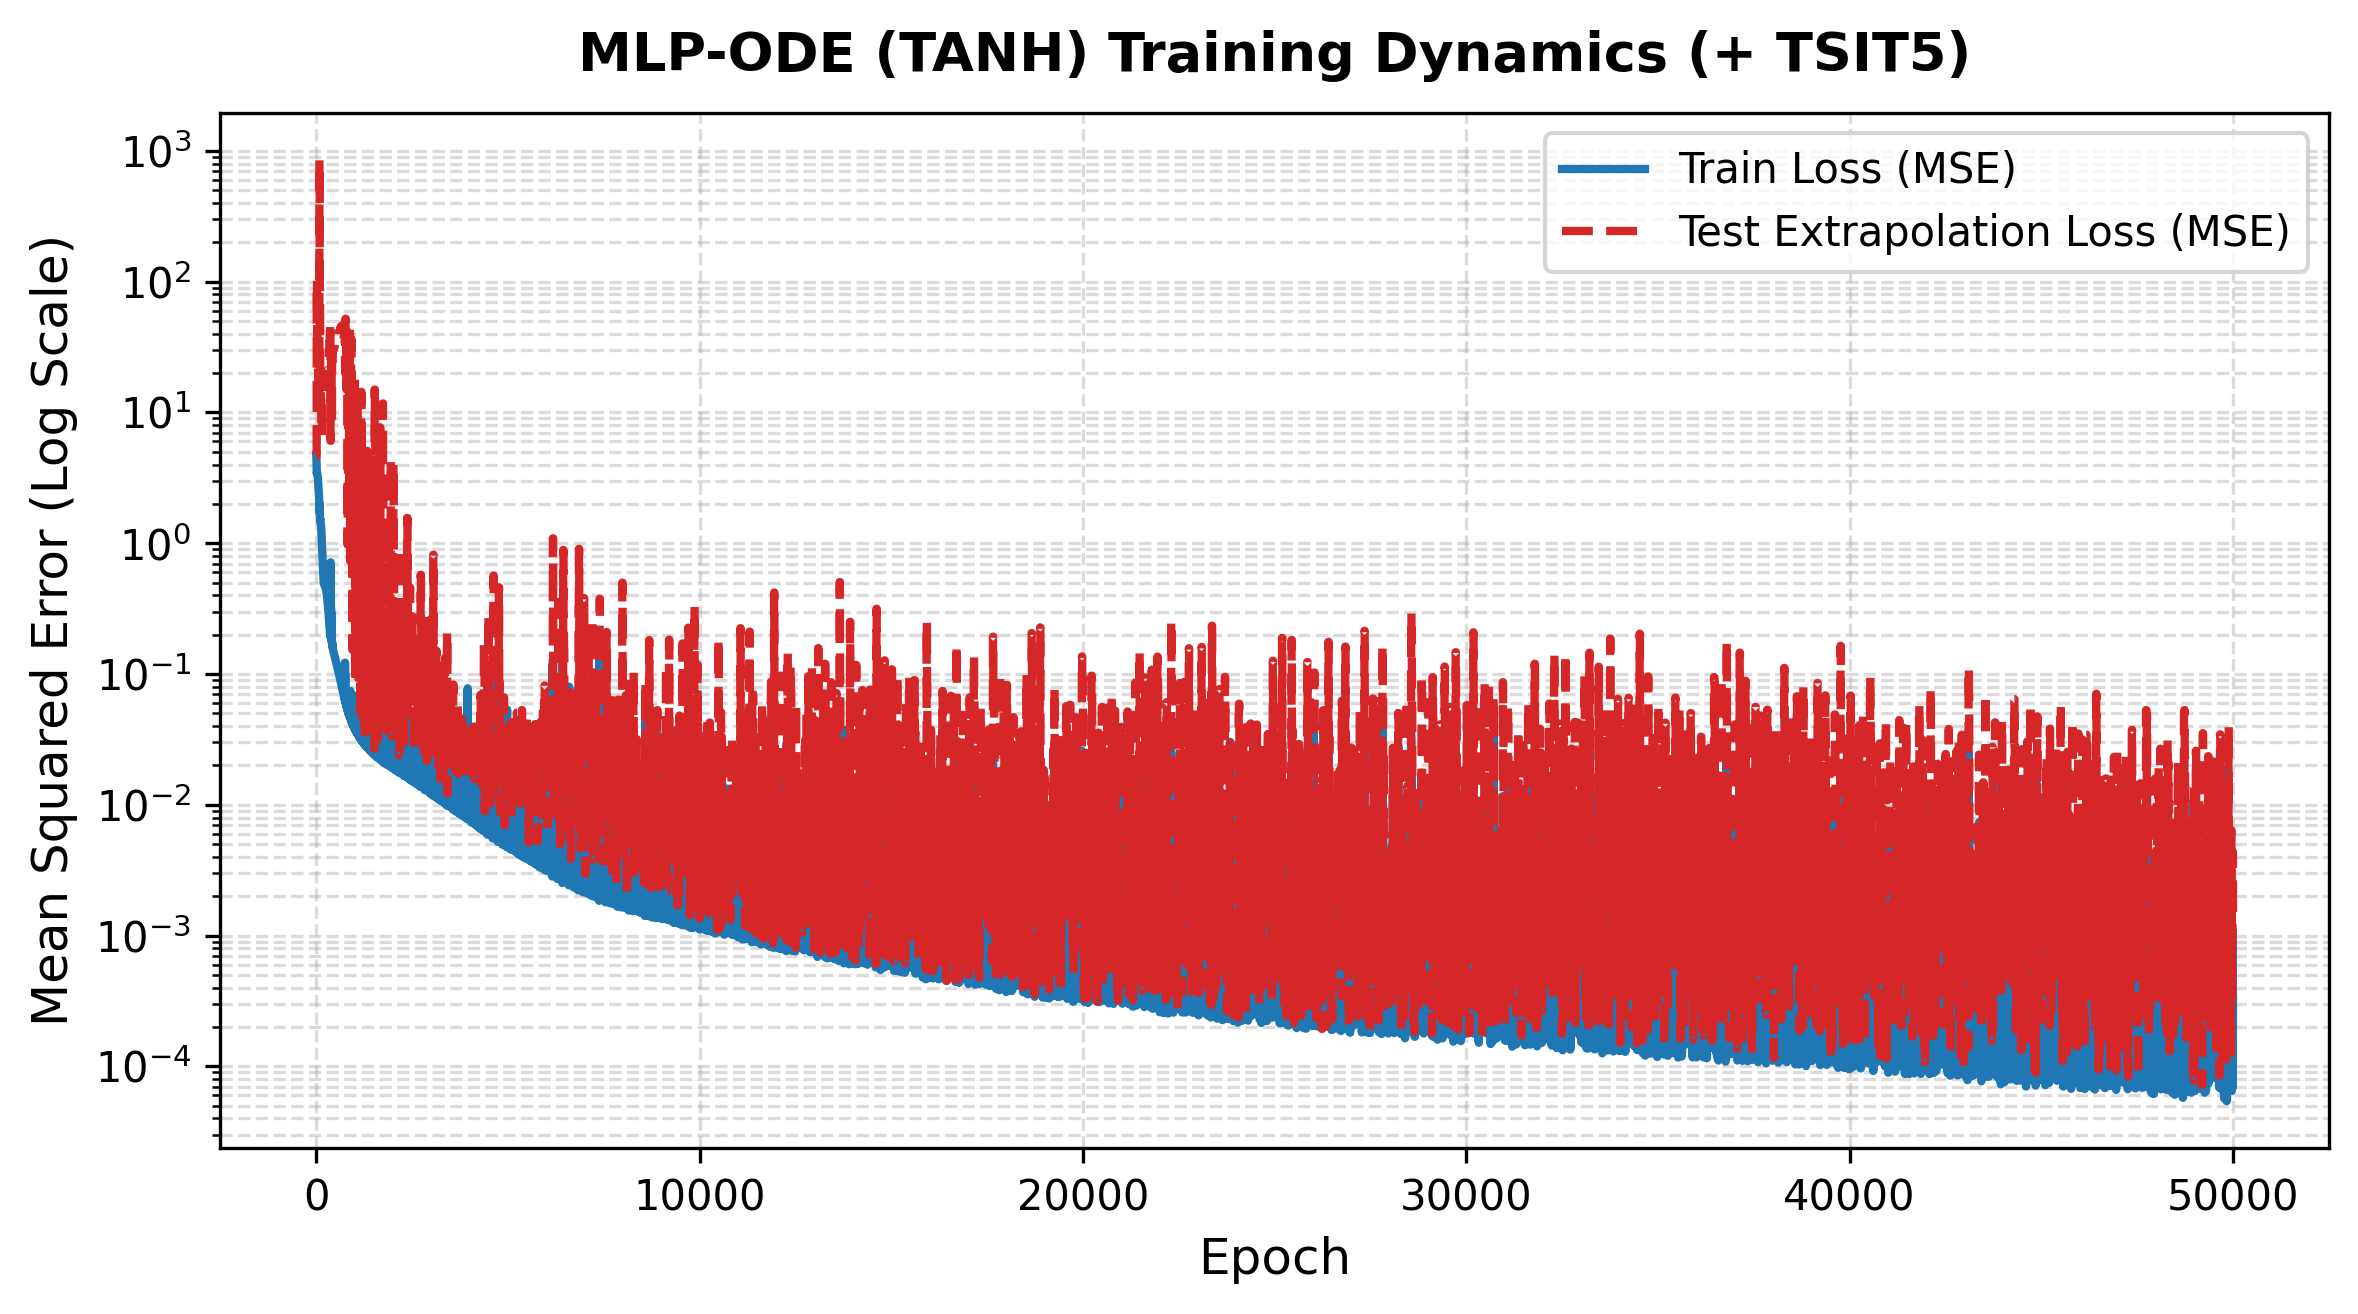
\includegraphics[width=\linewidth]{figures/phase4/mlp_tanh_exact_50k_loss_curves.png}
  \caption{MLP-ODE, tanh (paper's own lr/init), 50k}
\end{subfigure}
\caption{Training and test loss of the six extended runs, as saved by each
run. Training loss is logged every epoch; the test loss (full horizon
$[0,14]$) every ten epochs, and it spikes by up to two orders of magnitude
throughout, which is why the comparison in the text uses a 500-epoch rolling
median rather than raw values. Panel (f) shows the identical $[2,50,2]$ tanh
architecture of panel (e), retrained with only the learning rate and
initialization scale changed to the values in the paper's own published
code.}
\label{fig:phase4-curves}
\end{figure*}

Every working configuration improves its training MSE by $7.5$--$52\times$
(Table~\ref{tab:phase4}); what matters is which orderings survive.
Table~\ref{tab:phase4-verdicts} gives the verdict for each conclusion the
earlier sections draw.

\begin{table*}[t]
\centering
\footnotesize
\renewcommand{\arraystretch}{1.15}
\caption{Which $10^4$-epoch conclusions survive the extended budget.}
\label{tab:phase4-verdicts}
\begin{tabularx}{\textwidth}{@{}L{4.6cm} L{3.2cm} L{3.0cm} Y@{}}
\toprule
\hdrrow \thh{Conclusion at $10^4$ epochs} & \thh{At $10^4$} & \thh{At $5\times10^4$} & \thh{Verdict}\\
\midrule
RBF and B-spline are statistically tied & $6.1\%$ apart & $5.6\%$ apart (25k) & \textbf{Holds}. The basis choice can be made on cost.\\
Euler is the worst solver & $28.1\times$ Tsit5 & $4.8\times$ Tsit5 & \textbf{Holds}, with a much smaller margin: part of the gap was under-training.\\
The paper-spec MLP fails because of its architecture, not its budget & train $1.08$, $R^2=0.42$ & train $1.01$, $R^2=-0.48$ & \textbf{Budget part holds; architecture part reversed.} More epochs alone do not help, but the identical architecture trains under the paper's own learning rate and initialization (below): $R^2=0.9998$ at this budget.\\
KAN-ODE extrapolates better than a parameter-matched MLP & KAN $5.35\times$ better & MLP $6.82\times$ better & \textbf{Reverses.} The advantage is a budget effect.\\
\bottomrule
\end{tabularx}
\end{table*}

\paragraph{The paper-spec MLP is stuck, not slow.} With five times the
budget its training loss moves by $7\%$ ($1.083\to1.011$), its extrapolation
error rises $2.6\times$, and $R^2$ turns negative. The optimizer spends the
run in a pathological regime: clipping engages on $99.3\%$ of steps against
$2$--$11\%$ for every other configuration, the median pre-clip gradient norm
is $19.8$ against $0.03$--$0.17$, and the Lipschitz estimate nearly triples
to $104.8$, an order of magnitude above every other model. This settles half
of the question left open in Section~\ref{sec:kan-vs-mlp}: whatever is wrong
here is a property of this training run, not of the epoch count, since five
times the budget only entrenches it. It is not, however, a property of the
architecture itself. The next paragraph shows the identical network
training cleanly once its optimizer settings are corrected.

\paragraph{Resolving the audit's open optimizer row: the paper's own learning
rate and initialization.} The base paper's own published code (not
distributed with our project, but readable in its public repository) sets
two things differently for its MLP baseline than our default: a learning
rate of $10^{-2}$ (five times our $2\times10^{-3}$) and Glorot initial
weights divided by $10^5$, near zero rather than full-scale. Holding
architecture, activation, dataset, solver and seed fixed and changing only
those two settings, the identical $[2,50,2]$ tanh network trains cleanly at
both budgets (Table~\ref{tab:phase4}, row six; panel f of
Figure~\ref{fig:phase4-curves}). At $10^4$ epochs, training MSE falls from
$1.08$ to $1.11\times10^{-3}$ and extrapolation MSE from $1.69$ to
$9.65\times10^{-3}$ ($R^2:0.42\to0.997$). At $5\times10^4$ epochs training
MSE reaches $5.43\times10^{-5}$ and extrapolation MSE $4.31\times10^{-4}$
($R^2=0.99985$), against $1.01$ and $4.32$ under the default settings at the
same budget. Neither run needed gradient clipping or hit a single
non-finite gradient step. The conclusion Table~\ref{tab:mlp-breakdown} drew
does not survive this: changing only the learning rate and initialization
scale, with the exact literal architecture and activation that table showed
failing, is enough on its own. What that factorial actually measured was
sensitivity to activation \emph{at our optimizer settings}, not an
architecture-level incompatibility with the system.

Against the other two architectures at $5\times10^4$ epochs, the corrected
tanh MLP is still not competitive. Its extrapolation MSE
($4.31\times10^{-4}$) is $10.7\times$ KAN-ODE's and $73\times$ the SiLU MLP's,
and its learned equilibrium sits $1.72$ from the truth, the furthest of the
three (Table~\ref{tab:equilibria}). Its one advantage is conservation: a
first-integral drift of $0.06\%$ is the smallest of the three (KAN $0.08\%$,
SiLU-MLP $0.21\%$), though its on-orbit field error ($2.7\%$) is the
largest. It also falls short of the paper's own reported target. The paper
states that its MLP reaches a training loss of $3.0\times10^{-5}$ within
$10^5$ epochs; this run's training loss crosses $10^{-4}$ at epoch
$39{,}695$ but had not reached $3.0\times10^{-5}$ by epoch $50{,}000$. That
trend is consistent with, but does not confirm, the paper's own budget for
this baseline.

\paragraph{The KAN advantage over the MLP reverses.} At $10^4$ epochs, from
training losses $7\%$ apart, the KAN-ODE extrapolates $5.35\times$ better
than the SiLU MLP, the result that reproduces the paper's accuracy claim. At
$5\times10^4$ epochs the MLP's extrapolation MSE is $5.90\times10^{-6}$ and
the KAN's $4.02\times10^{-5}$: the MLP is $6.82\times$ better, far outside
the single-seed noise that separates RBF from B-spline. The checkpoint
analyses of Section~\ref{sec:numerics} agree on every measure. At 50k the MLP
has the smaller on-orbit field error ($0.6\%$ against $1.1\%$), the smaller
first-integral drift ($0.4\%$ against $0.9\%$), an equilibrium closer to the
truth ($0.68$ against $1.65$ away), and a lower far-horizon error
(maximum $2.4\times10^{-2}$ against $6.5\times10^{-2}$ on $(14,28]$). The
crossover is late. Smoothing the logged full-horizon MSE of
Figure~\ref{fig:phase4-curves} with a 500-epoch rolling geometric median,
the two models are level at $2.5\times10^4$
epochs ($1.7\times10^{-4}$ against $2.0\times10^{-4}$), and the MLP stays
ahead for good only from about epoch $48{,}500$. The MLP is also the faster
learner at every threshold: in the extended runs it reaches $10^{-4}$
training MSE at epoch 5225 against the KAN's 5695, and $10^{-5}$ at 13{,}815
against 31{,}412.

The honest reading is that KAN-ODE has a strong \emph{early} inductive bias
for this smooth periodic problem. Within a fixed, moderate budget it produces
the better extrapolator, but it is not the better function class once both
models are trained to convergence. Neither model learns the conservative
structure of the system (Figure~\ref{fig:limit-cycle}); the MLP simply fits
the training orbit's phase more precisely in the end.

\subsection{Comparison with the base paper}
\label{sec:audit}

This subsection gathers, in one place, how our results line up with the
base paper \cite{Koenig_2024}. We first compare our recipe with the
paper's stated methodology field by field
(Table~\ref{tab:audit}), so that no difference is silently absorbed into
``the paper trained longer''. The table uses the settings recorded in our
own planning notes and code, and marks as open every field those do not
determine. One such
field, the MLP baseline's optimizer settings, we later resolved by reading
the paper's own published code, which is how the follow-up runs of
Section~\ref{sec:phase4} came about.

\begin{table*}[t]
\centering
\footnotesize
\renewcommand{\arraystretch}{1.15}
\caption{Field-by-field comparison with the base paper \cite{Koenig_2024}.}
\label{tab:audit}
\begin{tabularx}{\textwidth}{@{}L{2.7cm} L{4.2cm} L{4.2cm} Y@{}}
\toprule
\hdrrow \thh{Field} & \thh{Base paper} & \thh{Ours} & \thh{Verdict}\\
\midrule
KAN architecture & $[2,10,2]$, $G=5$, 240 parameters & identical & Matches.\\
Edge basis & Gaussian RBF, $\exp(-r^2/2h^2)$ & identical, after fixing a missing factor $\tfrac12$ & Matches. The fix predates every reported run.\\
MLP baseline & $[2,50,2]$, tanh, 252 parameters & identical, plus a working $[2,14,8,8,2]$ SiLU variant & Matches literally, and trains under the paper's own optimizer settings (below).\\
Integrator & adaptive Tsit5 (Julia) & fixed-step Tsit5, $h=0.05$ & Explained: the fixed step's own error is $4.7\times10^{-14}$ in MSE (Table~\ref{tab:solver-ablation}).\\
Gradients & continuous adjoint & direct autograd & Explained: they differ in memory and time, not in the loss minimised (Section~\ref{sec:track-a}).\\
Framework & compiled Julia / SciML & interpreted PyTorch, CPU & Explained: wall-clock is not comparable across the two (Section~\ref{sec:budget}).\\
Epoch budget & $10^4$ (KAN), $10^5$ (MLP) & $10^4$, and $5\times10^4$ in Section~\ref{sec:phase4} & Explained: Section~\ref{sec:phase4}.\\
Optimizer, learning rate (MLP baseline) & Adam, $10^{-2}$, Glorot init $\div\,10^5$, found in the paper's own published code & Adam, $2\times10^{-3}$ by default, Glorot gain $1.0$, clip $1.0$ & \textbf{Resolved}: this mismatch, not the architecture, caused the earlier training failure. The paper's own KAN learning rate remains unconfirmed.\\
Loss normalisation & not recorded & mean over points and components & \textbf{Open}; affects absolute loss values only.\\
\bottomrule
\end{tabularx}
\end{table*}

\paragraph{The efficiency claim.} The paper reports its KAN-ODE reaching a
training loss of $2.6\times10^{-5}$ in $10^4$ epochs and its MLP needing
$10^5$ epochs for $3.0\times10^{-5}$. Our extended runs locate both targets
directly. Our KAN-ODE reaches $2.6\times10^{-5}$ at epoch $13{,}632$,
within $1.4\times$ of the paper's KAN. Our SiLU MLP reaches
$3.0\times10^{-5}$ at epoch $8{,}585$, nearly $12\times$ sooner than the
paper's MLP. The literal $[2,50,2]$ tanh MLP never gets below $1.0$ under
our default optimizer settings, but under the paper's own learning rate and
initialization it crosses $10^{-4}$ at epoch $39{,}695$ and had not reached
$3.0\times10^{-5}$ by epoch $50{,}000$: a trend consistent with, but short
of confirming, the paper's own $10^5$-epoch target. Allowing for the open
loss-normalisation row, the KAN side of the efficiency claim is reproduced.
The tenfold advantage over the literal MLP baseline, however, depends on
that baseline's optimizer settings as much as on its architecture, since the
identical network trains once those settings are corrected.

\paragraph{The accuracy claim.} At the paper's own $10^4$-epoch budget we
reproduce the extrapolation advantage: KAN-ODE is $5.4\times$ better than a
parameter-matched MLP (Section~\ref{sec:kan-vs-mlp}), and the gap widens to
$40.6\times$ at twice the horizon (Section~\ref{sec:crossdomain}). At five
times that budget the ranking reverses and the MLP is $6.8\times$ better
(Section~\ref{sec:phase4}), so we read the paper's accuracy claim as a
statement about moderate training budgets rather than about the two
function classes at convergence.

\paragraph{The three fixed design choices.} None of the paper's three fixed
choices turns out to be load-bearing on this benchmark. Tsit5 is not needed
for accuracy: above order two, every solver lands within $3.8\%$ of the
others, and Midpoint matches Tsit5 at $29\%$ of the cost
(Section~\ref{sec:solver-results}). The switch from B-spline to RBF is
justified on cost rather than accuracy: the two are statistically tied at
both budgets, with RBF $3.9\times$ cheaper per epoch
(Section~\ref{sec:basis-results}). And the adjoint method's memory saving,
while real at every trajectory length we tested, never matters at our
scale, while it costs $1.9$--$2.1\times$ in wall-clock
(Section~\ref{sec:track-a}).

\paragraph{Wall-clock.} Our absolute training times are not comparable with
the paper's. Our integration loop runs uncompiled in PyTorch on CPU,
whereas the paper compiles its loop in Julia's SciML ecosystem
(Table~\ref{tab:cost}). All our timing comparisons are therefore made only
between our own runs, on the same hardware.

\begin{keypoint}[Outcome of the comparison]
The $10^4$-epoch budget gives trustworthy \emph{rankings} for the solver and
basis ablations: the RBF/B-spline tie and Euler's last place both survive
five times the budget. It does not for the KAN-versus-MLP comparison, which
reverses: the paper's extrapolation advantage is an early-training effect
under our protocol, and its speed advantage over the literal MLP baseline
depended on that baseline's default optimizer settings, not on its
architecture. Corrected, the identical network trains, though it still does
not close the gap with either KAN-ODE or the SiLU MLP within our budget.
Every result is single-seed.
\end{keypoint}

\subsection{Discussion}
\label{sec:discussion}

Eight patterns recur across studies that were designed independently and
address unrelated questions. That they recur is itself informative about how
this class of model should be studied going forward.

\paragraph{A trained Neural ODE models its training orbit and its solver, not
the vector field.} The numerical analysis of Section~\ref{sec:numerics}
found this in three independent ways. First, the Euler-trained network is an
accurate model of the inverse modified equation, and no model transfers
across solver families (Figure~\ref{fig:cross-solver}). Second, every trained
model, KAN or MLP, at either budget, has an attracting limit cycle through
the training data around a spurious unstable equilibrium $1.2$--$1.7$ away
from the true one, where Lotka-Volterra has a neutral centre. Third, the
field is accurate only in a thin tube around the observed orbit
(Figure~\ref{fig:field-error}). Low trajectory error on the training orbit's
continuation is therefore compatible with a qualitatively wrong phase
portrait. Checks that probe the field directly, such as locating its
equilibria, integrating from new initial conditions or evaluating a known
invariant, are cheap once a checkpoint exists. They should be part of the
protocol whenever a learned field is to be read as physics.

\paragraph{Architecture comparisons are budget-dependent.} The
KAN-versus-MLP ranking reversed between $10^4$ and $5\times10^4$ epochs
(Section~\ref{sec:phase4}), while the solver and basis rankings did not. The
difference is instructive. The solver and basis comparisons are between
models of the same function class, and they were decided by truncation error
or locality, properties that do not change with training time. The
architecture comparison is between two function classes that converge at
different rates, and a fixed budget measures the rates as much as the
limits. A claim that one architecture ``generalises better'' should state
the budget, or better, report the error against training time for both.

\paragraph{A reasoned hypothesis still requires a control arm.} Three separate
studies advanced a specific, mechanistically plausible hypothesis and then
tested it directly: gradient-norm roughness as the cause of Euler's
convergence floor (Section~\ref{sec:track-b}), SiLU's representational limit
as the cause of the pendulum's early failure (Section~\ref{sec:crossdomain}),
and the predicted inapplicability of the vanishing-field gate to
non-mechanistic data (Section~\ref{sec:track-e}). Each hypothesis had a clear
argument behind it before any run was launched, and each was overturned by
the run itself. In all three cases the result we report is the outcome of
the control arm; the original argument survives only as the motivation for
running it. This is not a coincidence of three unlucky guesses. It reflects
the difficulty of reasoning about a system where the integrator, the
optimizer, and the learned function interact inside the same backpropagation
graph. The standard practice of ablating one variable while holding others
fixed rests on an assumption of near-independence that does not hold here.

\paragraph{A single seed and a single train/test split account for results
that first looked like properties of the solver or the method.} The
stiffness-map failures at $\mu\in\{0.5,1.0,2.0\}$ (Section~\ref{sec:track-d})
and the epidemic-fit extrapolation runaway (Section~\ref{sec:track-e}) both
appeared, on first inspection, to indict a solver or a modeling approach.
Retraining with additional seeds in the stiffness-map case, and shifting the
train/test split by fifteen days in the epidemic case, resolved both into an
artifact of one run's random initialization or one window boundary. Neither
observation survives as a claim about solver order or about KAN-ODE's
capacity once the seed or the split is varied. Every quantitative result we
report remains $N=1$. The stiffness study's small extension to $N=3$ was
enough to dissolve a headline finding, which underscores how much of the
rest of our work rests on the same single-seed foundation.

\paragraph{Measuring a quantity before training is more informative than
tuning after a failed run.} The SIR divergence (Section~\ref{sec:crossdomain}),
the epidemic-curve fit (Section~\ref{sec:track-e}), and the stiffness map's
spurious equilibrium (Section~\ref{sec:track-d}) were each root-caused by
evaluating the model's own initial field, or its trained field at a candidate
equilibrium, and comparing that number against the system's true scale. In
every case this produced a specific, falsifiable prediction (a rescaling
factor, a fix that should or should not transfer, an equilibrium location)
that a short follow-up run confirmed or refuted directly. A hyperparameter
sweep would instead have required an open-ended search.

\paragraph{Training accuracy and generalization quality are decoupled.} The
hybrid basis matches pure RBF's training loss to $1.7\%$ at 10{,}000 epochs
yet collapses in extrapolation ($R^2=-2.17$ vs.\ $+0.647$,
Section~\ref{sec:track-c}). The stiffness map's trapped models
(Section~\ref{sec:track-d}) reach training losses of $1.8\times10^{-2}$,
qualitatively acceptable on a casual inspection, while their learned field
has a large nonzero derivative at the true equilibrium. And the
epidemic-curve model (Section~\ref{sec:track-e}) produces a plausible
training fit while predicting an infected peak six times the physical
maximum. In all three cases, a reader who judged the model solely by
training-window MSE would reach the wrong conclusion. We adopted the
evaluation protocol of Section~\ref{sec:protocol} (scoring strictly on
extrapolation, never on training loss) precisely because we anticipated this
decoupling. These studies go further: they show that configurations
differing by two orders of magnitude in extrapolation quality can produce
numerically indistinguishable training fits. The number to watch is always
the one computed outside the training window, and no training-window metric
we tested reliably predicts it.

\paragraph{Cost and accuracy form a clear Pareto frontier.} Across the
solver ablation (Section~\ref{sec:solver-results}, Figure~\ref{fig:pareto}),
the basis ablation (Section~\ref{sec:basis-results}), and the hybrid-basis
study (Section~\ref{sec:track-c}), a consistent pattern emerges: the
cheapest methods that work (Midpoint at $1/3$ the function evaluations of
Tsit5; RBF at $1/3.9$ the wall-clock of B-spline) match the accuracy of
their more expensive alternatives to within single-seed noise. Adding cost,
whether more function evaluations per step, more basis evaluations per
edge, or a second basis evaluated in parallel, does not buy a measurable
accuracy improvement on any system tested. The hybrid-basis result makes
this particularly sharp: the blend pays roughly the sum of both bases'
per-epoch compute for two extra parameters and never recovers the cost in
accuracy.

\paragraph{These KAN edges do not produce interpretable symbolic structure
without explicit encouragement.} The pruning experiment
(Section~\ref{sec:track-e}) found that removing the two weakest of forty edges
degrades a noise-free model to worse than a constant predictor, a factor of
$3.9\times10^4$. Every edge carries part of the fit, the magnitude ranking
is close to arbitrary, and no edge can be identified with a specific term in
the governing equation. This is a direct consequence of training without
sparsity-inducing regularization. It means the interpretability advantage
that motivated the original choice of a smooth, globally-supported basis
function remains a hypothesis rather than a demonstrated property of our
trained models. A future retraining with explicit edge-level regularization
would be needed to test whether sparse, readable edge functions emerge when
the training loss actively asks for them.



\section{Conclusion and Future Work}
\label{sec:conclusion}
We reproduced the KAN-ODE recipe of the base paper on the Lotka-Volterra
system with every integrator and basis implemented from its defining formula
and verified numerically. We then extended the recipe to a damped pendulum
and an SIR epidemic model, diagnosed and fixed two genuine cross-domain
training failures, ran five follow-on studies that each isolate one
question, and re-tested the budget-sensitive conclusions at five times the
training budget. Every quantitative claim traces to a saved training record, a
re-scored checkpoint or a regenerable figure (Appendix~\ref{app:repro}).

\subsection{Key takeaways}

\begin{itemize}[leftmargin=1.2em]
\item \textbf{Solver order matters only up to two.} All six integrators
  satisfy their order conditions to round-off (37 rooted trees checked).
  Above order two the solver does not change accuracy at the training step,
  and Midpoint matches Tsit5 within $0.3\%$ at $29\%$ of the wall-clock.
\item \textbf{The network learns the field its solver needs.} The Euler
  model matches the inverse modified equation
  $\mathbf{f}+\tfrac{h}{2}J\mathbf{f}$ (cosine $0.92$, magnitude ratio
  $1.04$), and models lose one to four orders of magnitude when integrated
  with a solver from another family.
\item \textbf{Trained models learn an orbit, not the vector field.} Every
  trained model, KAN or MLP, is an attracting limit cycle around a spurious
  unstable equilibrium, where Lotka-Volterra has a neutral centre; the field
  is accurate only in a thin tube around the training orbit.
\item \textbf{Locality, not conditioning, separates the bases.} B-spline and
  RBF are tied at both budgets, and the global polynomials extrapolate
  $4$--$5\times$ worse. Extrapolation MSE scales as $12.9\,\sigma^{2.02}$
  with observation noise.
\item \textbf{KAN-ODE's advantage over the MLP is budget-dependent.} At
  $10^4$ epochs KAN-ODE extrapolates $5.4\times$ better than a
  parameter-matched MLP (widening to $40.6\times$ at twice the horizon); at
  $5\times10^4$ epochs the MLP is $6.8\times$ better. The paper's literal
  tanh MLP trains once given the paper's own learning rate and
  initialization.
\item \textbf{Measure before you tune.} SIR's failure traced to a $19\times$
  unit-scale mismatch at initialization. A change of time units and a
  conservation projection remove the divergence, and a vanishing-field gate
  brings extrapolation $R^2$ from $-20.97$ to $+0.9981$.
\item \textbf{Follow-on studies.} Direct autograd is the right default at
  our scale (the adjoint saves memory but costs $1.9$--$2.1\times$ in time);
  gradient roughness does not explain Euler's floor ($\rho=-0.088$); a
  learnable spline/RBF blend never beats the better pure basis;
  stiffness-map failures trace to the random seed; and sparse regression is
  far more noise-robust than KAN-ODE ($9\times$ vs.\ $1540\times$
  degradation) but less accurate at every noise level.
\end{itemize}

\subsection{Limitations}

\begin{itemize}[leftmargin=1.2em]
\item \textbf{Single seed.} Every configuration was trained with one random
  seed. The stiffness study, where going from one seed to three dissolved a
  headline finding, shows how much this can matter.
\item \textbf{Single train/test split.} Most results use one split per
  system; on the epidemic curve, moving the split by fifteen days changed
  the conclusion.
\item \textbf{Timing comparability.} Our loop runs uncompiled in PyTorch, so
  our wall-clock numbers compare our own configurations with each other but
  not with the base paper's Julia implementation.
\item \textbf{Explicit solvers, fixed steps.} We implemented only explicit
  Runge-Kutta methods at a fixed step; we cannot say how an implicit or
  adaptive solver would behave on a genuinely stiff system.
\item \textbf{No sparsity pressure.} All models were trained with
  $\lambda=0$ in Equation~\ref{eq:l1-sparsity}, so our pruning results say
  nothing about how interpretable a sparsity-regularised KAN-ODE would be.
\item \textbf{Synthetic epidemic curve.} The outbreak curve is synthetic
  rather than observed case data.
\end{itemize}

\subsection{Future work}

The most valuable next experiment is multi-seed replication of the
KAN-versus-MLP crossover, since it is the one conclusion that reversed with
budget. Two cheaper follow-ups come straight out of the numerical analysis:
an affine input normalisation that uses the whole first-layer grid on
positive-valued systems, and training from several initial conditions, the
most direct way to ask a Neural ODE for the vector field rather than a
single orbit. Retraining with the $L_1$ penalty of
Equation~\ref{eq:l1-sparsity} would test whether readable edge functions
emerge when the loss asks for them, and fitting observed outbreak data would
complete the epidemic transfer test.


\begin{acks}
We thank our supervisor, Niaz Rahman (Lecturer, Department of CSE, BUET),
for his guidance throughout this project.
\end{acks}

\bibliographystyle{ACM-Reference-Format}
\bibliography{references}

\appendix
% Label appendix sections "Appendix A" (subsections keep "A.1", ...).
\makeatletter
\def\kk@appendixprefix@section{Appendix~}% expandable: no \def inside the format
\def\@seccntformat#1{%
  \ifcsname kk@appendixprefix@#1\endcsname\csname kk@appendixprefix@#1\endcsname\fi
  \csname the#1\endcsname\quad}
\makeatother
\section{Reproducibility}
\label{app:repro}

\subsection{Environment and settings}

\begin{itemize}[leftmargin=*,itemsep=1pt,topsep=2pt]
\item \textbf{Code.} The integrators, bases, models, training loop and
  analysis pipeline are in the repository linked in the abstract, together
  with every checkpoint and training history the report uses. The analysis
  pipeline lives in \texttt{report/reproduce/}; its README gives the single
  command that reruns it and lists what each step reads and writes.
\item \textbf{Software and hardware.} Python and PyTorch, CPU only, float32
  throughout. Runs were trained on two Windows~11 machines and on Linux cloud
  (Kaggle) CPUs, under PyTorch 2.5 to 2.13; each run records its full
  configuration, PyTorch version, platform and code commit with its metrics.
\item \textbf{Data.} Every system's ground truth is solved with SciPy's
  DOP853 at $\text{rtol}=\text{atol}=10^{-12}$. Lotka-Volterra is sampled
  every $\Delta t=0.1$:
  36 training points on $[0,3.5]$ and 141 points on $[0,14]$, the last
  105 of which form the extrapolation test set.
\item \textbf{Seeding.} Seed 42 for every run except the extra stiffness
  seeds (1 and 7). The seed is set before the data are generated and again
  before the model is built, so the initialization depends on the seed alone.
\item \textbf{Model selection.} The reported checkpoint is the one with the
  lowest training MSE; the extrapolation window is never used to choose it.
\item \textbf{Cost.} The analysis pipeline takes a few minutes on a laptop
  CPU and retrains nothing; retraining all 24 Lotka-Volterra configurations
  takes about 14 CPU-hours (Table~\ref{tab:cost}).
\end{itemize}

\subsection{How the numbers and figures are regenerated}

Every training run saves its final metrics, a per-epoch training history, and
two checkpoints: the one with minimum training loss and the final one. A
single command-line entry point trains any configuration (model type, basis,
solver, sub-steps, learning rate, epoch budget and seed), and a separate
script re-scores any saved checkpoint against the ground truth it was
trained on. The extended runs of the budget validation were launched as
independent cloud jobs with the same entry point; the paper-settings tanh
MLP used a separate script, as the entry point does not expose the
initialization scale.

Everything reported after training is produced by an analysis pipeline that
retrains nothing. Its first step re-integrates every noise-free
$\Delta t=0.1$ checkpoint and checks that the rollout reproduces the run's
stored extrapolation MSE (the worst relative deviation is
$6.2\times10^{-3}$, from cloud-trained checkpoints re-scored on a different
CPU). The remaining steps compute the order conditions, work-precision data,
stability regions, Newton equilibria, first-integral drift, cross-solver
matrix, field-error maps and training milestones reported in
Sections~\ref{sec:solver-results}--\ref{sec:numerics} and~\ref{sec:phase4}.
Table~\ref{tab:provenance} lists what each derived figure and table is
computed from.

\begin{table}[t]
\centering
\footnotesize
\setlength{\tabcolsep}{4pt}
\renewcommand{\arraystretch}{1.08}
\caption{What each figure and table produced after training is computed from.}
\label{tab:provenance}
\begin{tabularx}{\columnwidth}{@{}L{4.1cm} Y@{}}
\toprule
\hdrrow \thh{Figure or table} & \thh{Computed from}\\
\midrule
Tables~\ref{tab:solver-ablation}, \ref{tab:basis-ablation}, \ref{tab:noise-dt}, \ref{tab:kan-vs-mlp}, \ref{tab:cost}, \ref{tab:phase4} & saved final metrics of each run\\
Table~\ref{tab:order-conditions} & the implemented solver tableaux\\
Figure~\ref{fig:work-precision}, truncation column of Table~\ref{tab:solver-ablation} & the true Lotka-Volterra field\\
Figure~\ref{fig:stability} & solver tableaux and the Tsit5 checkpoint\\
Figure~\ref{fig:basis-catalog}, $\kappa_2$ in Table~\ref{tab:basis-ablation} & the implemented basis functions\\
Table~\ref{tab:equilibria}, Figure~\ref{fig:first-integral} & trained checkpoints\\
Figure~\ref{fig:limit-cycle} & trained checkpoints\\
Figure~\ref{fig:cross-solver}, modified-equation analysis & checkpoints of the solver sweep\\
Figure~\ref{fig:field-error} & trained checkpoints\\
Figure~\ref{fig:edges} & RBF and B-spline checkpoints\\
Table~\ref{tab:milestones}, budget-validation crossover & per-epoch training histories\\
Figures~\ref{fig:kan-vs-mlp}, \ref{fig:kan-vs-mlp-t28}, Table~\ref{tab:extrap-horizon} & training histories; KAN, SiLU and paper-tanh checkpoints\\
Figure~\ref{fig:pareto} & saved final metrics of each run\\
Figure~\ref{fig:noise-dt} (right) & runs of the noise sweep\\
Figure~\ref{fig:error-vs-time} & trained checkpoints\\
Diagrams (Figures~\ref{fig:kan-ode-architecture}, \ref{fig:kdense}, \ref{fig:data-split}, \ref{fig:rk-stages}, \ref{fig:locality}) & drawn from the implemented coefficients and shapes\\
\bottomrule
\end{tabularx}
\end{table}

\subsection{The integrator implementation}

The fixed-step Tsit5 step and the trajectory integrator, with docstrings
shortened. Every other method follows the same pattern with its own
tableau.

\begin{pycode}[Fixed-step Tsit5 step]
def step_tsit5(func, t, y, dt):
    # 6 of 7 stages: the 7th (FSAL) stage has TSIT5_B[6] == 0.0
    k = []
    k.append(func(t, y))
    for stage_idx in range(1, 6):
        t_stage = t + TSIT5_C[stage_idx] * dt
        y_stage = y
        for j in range(stage_idx):
            y_stage = y_stage + dt * TSIT5_A[stage_idx][j] * k[j]
        k.append(func(t_stage, y_stage))
    y_next = y
    for j in range(len(k)):
        if TSIT5_B[j] != 0.0:
            y_next = y_next + dt * TSIT5_B[j] * k[j]
    return y_next
\end{pycode}

\begin{pycode}[Trajectory integrator]
def odeint(func, y0, t, method="tsit5", substeps=1):
    step_fn = STEP_SOLVERS[method.lower()]
    trajectory = [y0]
    curr_y = y0
    for i in range(len(t) - 1):
        dt_sub = (t[i + 1] - t[i]) / substeps     # h = dt / substeps
        for s in range(substeps):
            curr_t = t[i] + s * dt_sub
            curr_y = step_fn(func, curr_t, curr_y, dt_sub)
        trajectory.append(curr_y)
    return torch.stack(trajectory, dim=0)
\end{pycode}

Because the loop is ordinary PyTorch, reverse-mode differentiation of the loss
records every stage evaluation; this is the ``direct autograd'' gradient
method of Section~\ref{sec:track-a}, and the reason training cost is
proportional to the number of function evaluations.

\subsection{Order-condition check}

The verification of Table~\ref{tab:order-conditions} needs only the
tableau. Rooted trees are represented as sorted tuples of their subtrees;
for a tree $\tau=[\tau_1,\dots,\tau_m]$ the elementary weight vector is
$\mathbf{g}(\tau)=\prod_k A\,\mathbf{g}(\tau_k)$ (elementwise, with
$\mathbf{g}(\bullet)=\mathbf{1}$), the density is
$\gamma(\tau)=|\tau|\prod_k\gamma(\tau_k)$, and the condition is
$\mathbf{b}^\top\mathbf{g}(\tau)=1/\gamma(\tau)$.

\begin{pycode}[Order-condition check]
def elem_weight(t, A):
    g = np.ones(A.shape[0])
    for child in t:
        g = g * (A @ elem_weight(child, A))
    return g

def gamma_of(t):
    return order_of(t) * math.prod(gamma_of(c) for c in t)

for q in range(1, 7):                  # 1, 1, 2, 4, 9, 20 trees
    devs = [b @ elem_weight(t, A) - 1.0 / gamma_of(t) for t in trees[q]]
\end{pycode}


\end{document}
